\documentclass[11pt,nswissgerman]{article}
\usepackage{helvet}
\renewcommand{\familydefault}{\sfdefault}
\usepackage[utf8x]{inputenc}
\usepackage[a4paper]{geometry}
\geometry{verbose,tmargin=3cm,bmargin=3cm,lmargin=3.5cm,rmargin=3.5cm,headheight=3cm,headsep=1cm,footskip=2cm}
\usepackage{fancyhdr}
\pagestyle{fancy}
\usepackage[T1]{fontenc} %sollte bessere Zeilenumbrüche geben
\usepackage{titletoc}
\usepackage{wrapfig}
\usepackage{graphicx}
\usepackage{float}
\usepackage{tocbibind} %Damit erscheinen die Verzeichnisse im Inhaltsverzeichnis
\usepackage{epstopdf} %Packet um .eps Dateien einzubinden
\usepackage[position=bottom]{subfig}
\usepackage[colorlinks,
pdfpagelabels,
pdfstartview = FitH,
bookmarksopen = true,
bookmarksnumbered = true,
linkcolor = black,
plainpages = false,
hypertexnames = false,
urlcolor = green,
citecolor = black] {hyperref}
\makeatletter
\@ifundefined{date}{}{\date{}}
\makeatother
\usepackage{babel}
\setcounter{secnumdepth}{1} % levels under \section are not numbered
\setcounter{tocdepth}{2}    % levels under \subsection are not listed in the TOC

\begin{document}
\begin{titlepage}
\centering

\includegraphics[width=10cm]{../Bilder/Logo/Logo.png} \\
\vspace{2cm}
{\huge\bfseries Gesammelte Werke von jackthebus.com\par}
\vspace{2cm}
{\Large Stefan Bopp} \\
{\Large Chantal Frunz}
\vfill
{\large V2.0}
\thispagestyle{empty}

\end{titlepage}
\cleardoublepage
\newpage
\lhead{\leftmark}
\rhead{jackthebus.com}

\cfoot{\thepage}

\tableofcontents
\newpage
\section{Flims 2011}
%    JJJ    AA     CCCCCC KKK   K TTTTTT HH  HH EEEEEE BBBBBB UU  UU SSSSSS    CCCCCC OOOOOO MM  MM
%    JJJ   AAAA    CCCCCC KKK  K  TTTTTT HH  HH EEEEEE BB   B UU  UU SSS       CCCCCC OOOOOO MM  MM
%    JJJ  AA  AA   CC     KKK K     TT   HHHHHH EEE    BB   B UU  UU SSS       CC     OO  OO MMMMMM
%    JJJ AA    AA  CC     KKKK      TT   HHHHHH EEEEEE BBBBBB UU  UU  SSSSS    CC     OO  OO M MM M
%    JJJ AAAAAAAA  CC     KKK K     TT   HH  HH EEE    BB   B UU  UU    SSS    CC     OO  OO M MM M
% JJJJJJ AA    AA  CCCCCC KKK  K    TT   HH  HH EEEEEE BB   B UUUUUU    SSS .. CCCCCC OOOOOO M MM M
% JJJJJJ AA    AA  CCCCCC KKK   K   TT   HH  HH EEEEEE BBBBBB UUUUUU SSSSSS .. CCCCCC OOOOOO M MM M
% 
% Texte Geschrieben von Stefan Bopp und Chantal Frunz
% Mehr Informationen sind auf jackthebus.com zu finden

\subsection{Tag 1}

\begin{wrapfigure}{R}{0.45\textwidth} 
  \begin{centering}
    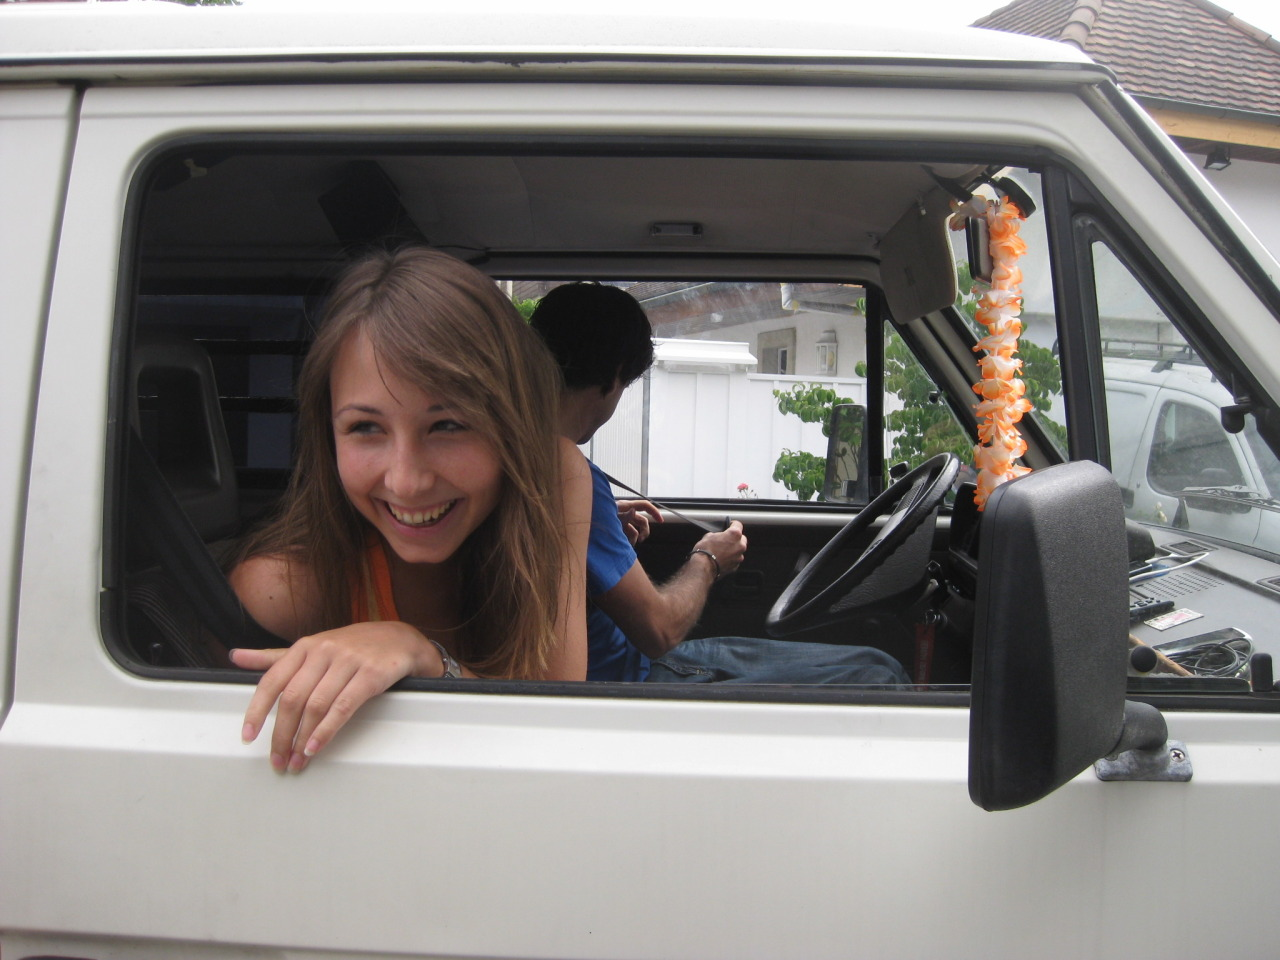
\includegraphics[width=0.4\textwidth, height=5cm, keepaspectratio]{../Bilder/Flims/2.jpg}
    \caption{Abfahrt}
  \end{centering}
\end{wrapfigure} 

\begin{figure}[b]
   \centering
      %\subfloat[CAPTION]{BILDERCODE}\qquad
   \subfloat{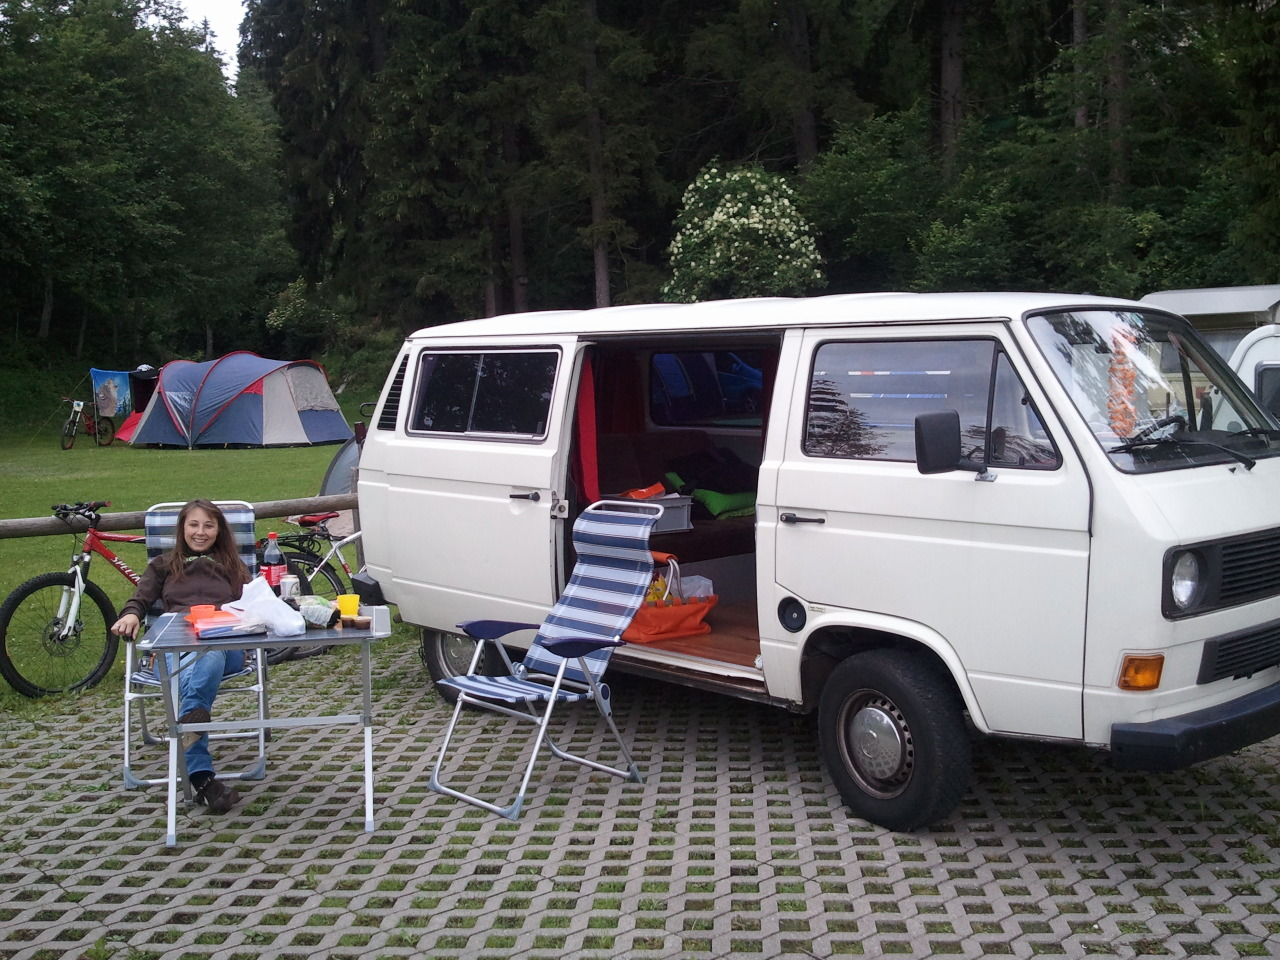
\includegraphics [width=0.3\textwidth]{../Bilder/Flims/4.jpg}}\quad
   \subfloat{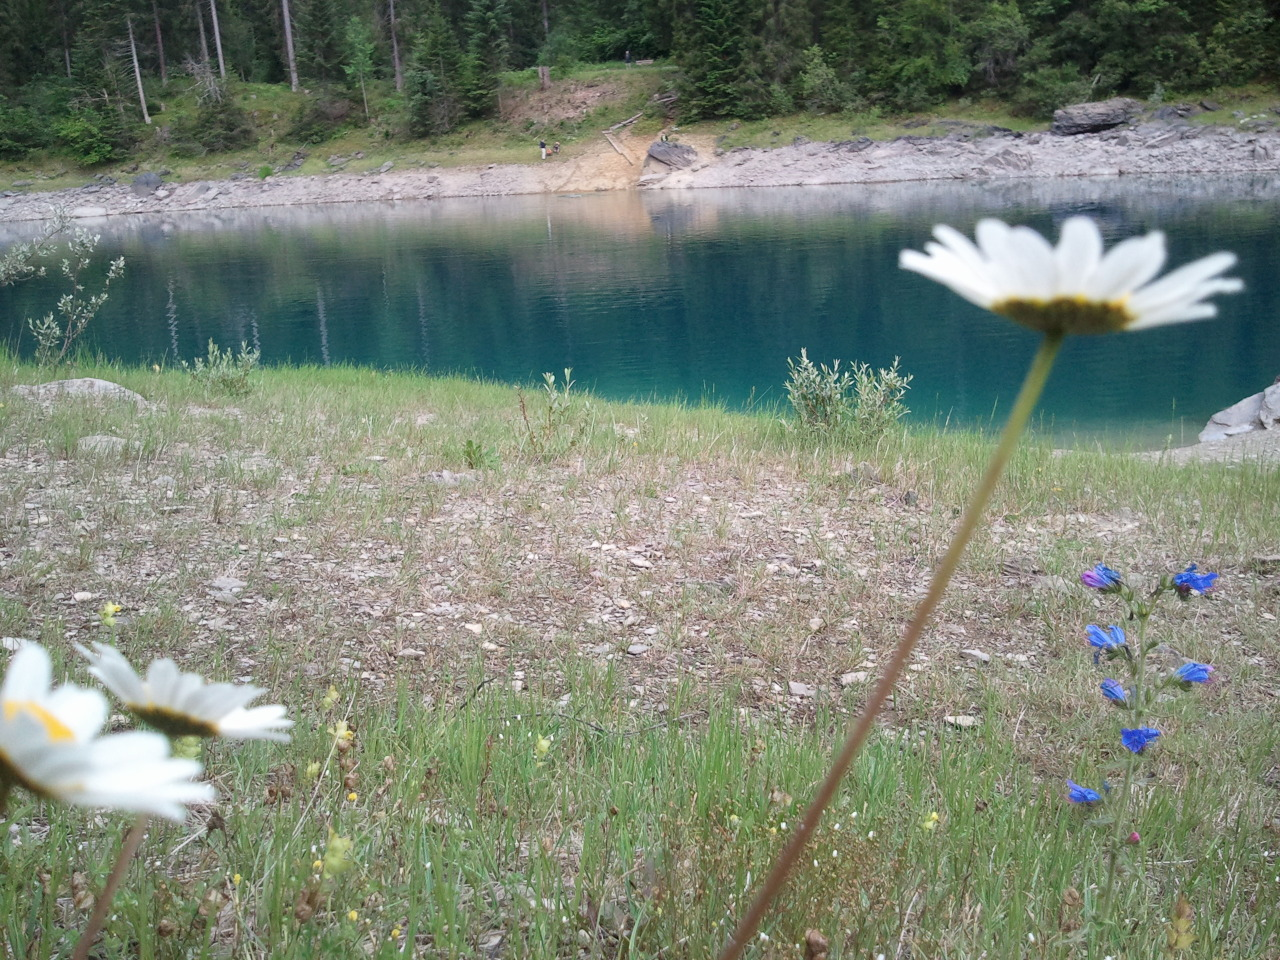
\includegraphics [width=0.3\textwidth]{../Bilder/Flims/8.jpg}}\quad
   \subfloat{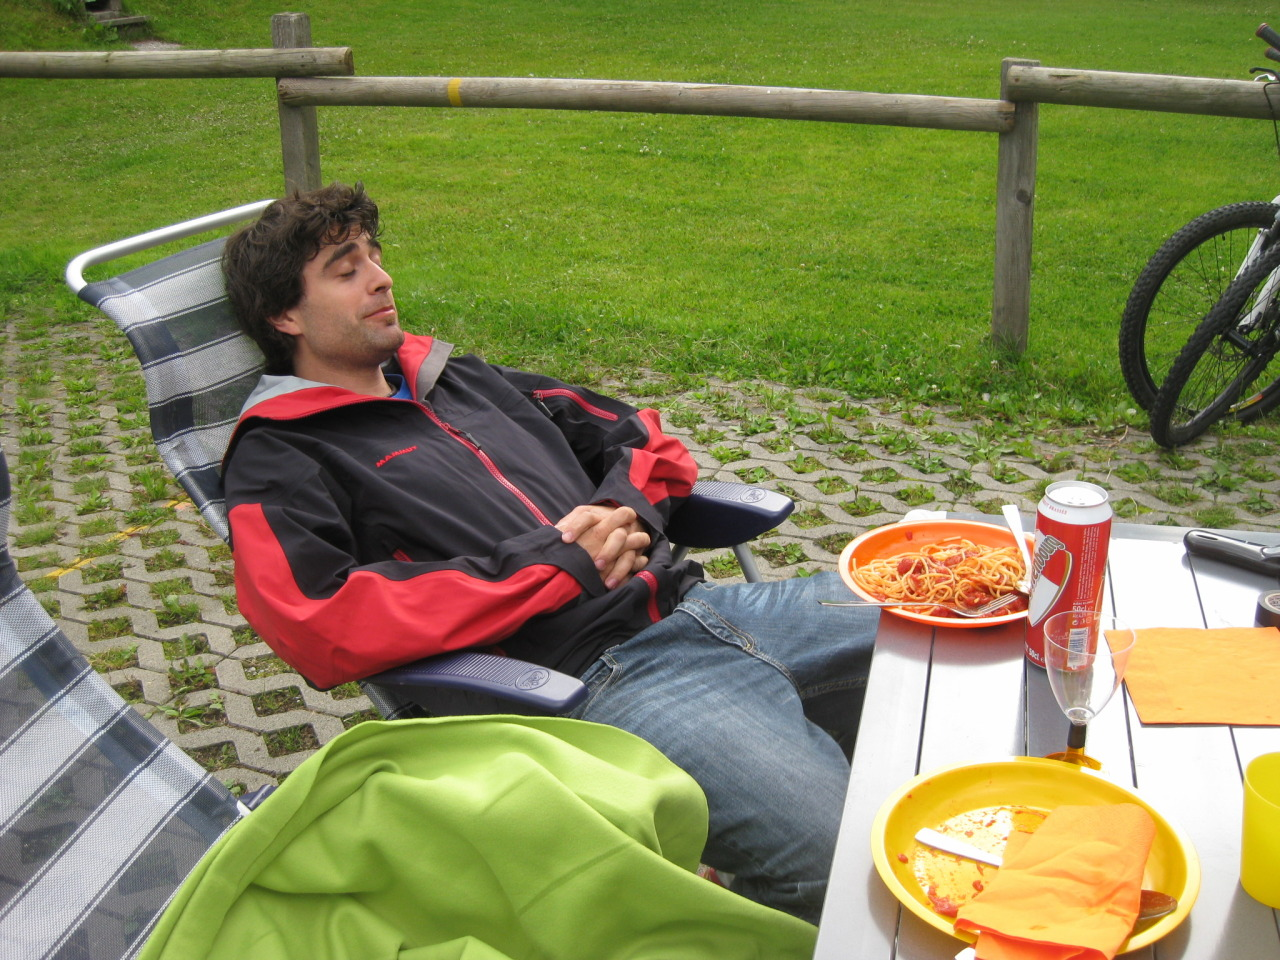
\includegraphics [width=0.3\textwidth]{../Bilder/Flims/15.jpg}}\quad
   \caption[Caumasee und Campingplatz]{Caumasee und Campingplatz}
\end{figure}

Als Geburtstagsgeschenk überraschte mich Chantal mit der frohen Nachricht, dass es am Samstag nach Flims gehen soll.
In Flims fand an diesem Weekend gerade auch noch der Trail Fox statt.
Perfekt für eine erste Probe des schon Geleisteten.
Geplant war die Abfahrt um spätestens halb 9.
Es kam jedoch anders als gedacht.
Wir brachen kurz nach 10 auf und waren um 10 nach 10 schon wieder zurück.
Meine Beifahrerin hat die falsche Schuhwahl getroffen.
Spätestens jetzt konnte uns nichts mehr aufhalten.

10 Minuten später...
Tank musste gefüllt werden.
Von nun an lief alles problemlos bis ins bekannte Heidiland.
Diesen Stopp benutzten wir um unsere Vorräte aufzufrischen und fuhren danach ohne weiteren Unterbruch auf den Campingplatz.
Leider war jedoch niemand an der Reception.
Daneben stand aber die Handynummer und so wurden wir telefonisch auf den Platz sieben gelotst.
Nun stand uns zum ersten Mal das aufstellen und bereitmachen des Buses bevor.
Stromversorgung funktionierte ohne zu murren und
auch der restliche Kram war schon jetzt in Rekordzeit aufgestellt.
Nach kurzer Verpflegung stand dem Spass in den Bäumen von Flims nichts mehr im Weg.
.. Seilpark wir kommen.
Jedoch hatte dieser am Samstag wegen dem Rennen nur bis vier Uhr offen.
Es blieb weniger als eine Stunde übrig und so beschlossen wir trotz bescheidenem Wetter den Cauma-See zu besuchen.
Nach unzähligen Fotos fing es leicht an zu Regnen.
In einer trockenen Pause radelten wir die 10 Minuten zum Campingplatz zurück.
Unterwegs sollte noch für das Abendessen eingekauft werden.
Wir trafen um 17:05 vor dem Volg ein, der natürlich um fünf Uhr schliesst.
In der modernen Zeit, in der wir leben ist es jedoch dank technischer Hilfsmittel problemlos möglich immer und überall einen der zahlreichen Tankstellenshops anzusteuern.
Sie stellen die Nahrungsmittelversorgung der zu spät kommenden sicher.
Auch in Flims gibt es solch einen Lebensretter.
Kurz per Google-Maps den Standort bestimmen und schon waren wir unterwegs Richtung Nahrung.
Eine Velotechnisch unfreundliche Autostrasse versperrte uns jedoch den Weg zum abendlichen Essensglück.
Jack war die Lösung.
Kurz alle Leitungen gekappt, die uns und Jack mit Energie versorgen und los ging die Fahrt in Schrittgeschwindigkeit durch die wahrhafte Flut von Dauercampern.
Das Loch im Auspuff macht sich in solch einer Situation sehr positiv bemerkbar: Vor den meisten voll verkleideten und eingezäunten Caravans sitzen regungslose Personen die einer schlechten Fasnachtspuppe gleichen.
Schon bei der ersten Fahrt zu unserem Platz spekulierten wir, welche von diesen Geschöpfen überhaupt noch am Leben sind.
Das leise Gluckern unseres VW Boxers unterstützt durch unregelmässige Fehlzündungen und mit sattem Bass aus dem Loch im Auspuff unterlegt, zwang diese Camper immerhin zu einem schiefen Blick, der als Lebenszeichen gedeutet werden konnte.
Die Tankstelle war dann schnell erreicht, jedoch wären doch einige Höhenmeter zu bezwingen gewesen um sie mit dem Fahrrad zu erreichen Das Kochen und der Abwasch ging Schulbuchmässig über die Bühne.
Chantal trumpfte sogar noch mit Champagner auf.
Jedoch vertrieb uns die kühle Brise schon sehr bald von unseren bequemen Stühlen.
Das Rennen am Abend wollten wir natürlich auch verfolgen.
So machten wir uns ein weiteres Mal Richtung Sportcenter, wo wir gerade noch die Aufräumarbeiten begutachten konnten.
Die Party, welche am Laufen sein sollte war auch nicht gerade der Bringer und so machten wir uns auf den Weg zurück in den Bus und genossen bis zum Einschlafen noch einen spannenden Film.

\subsection{Tag 2}
\begin{wrapfigure}{L}{0.45\textwidth} 
  \begin{centering}
    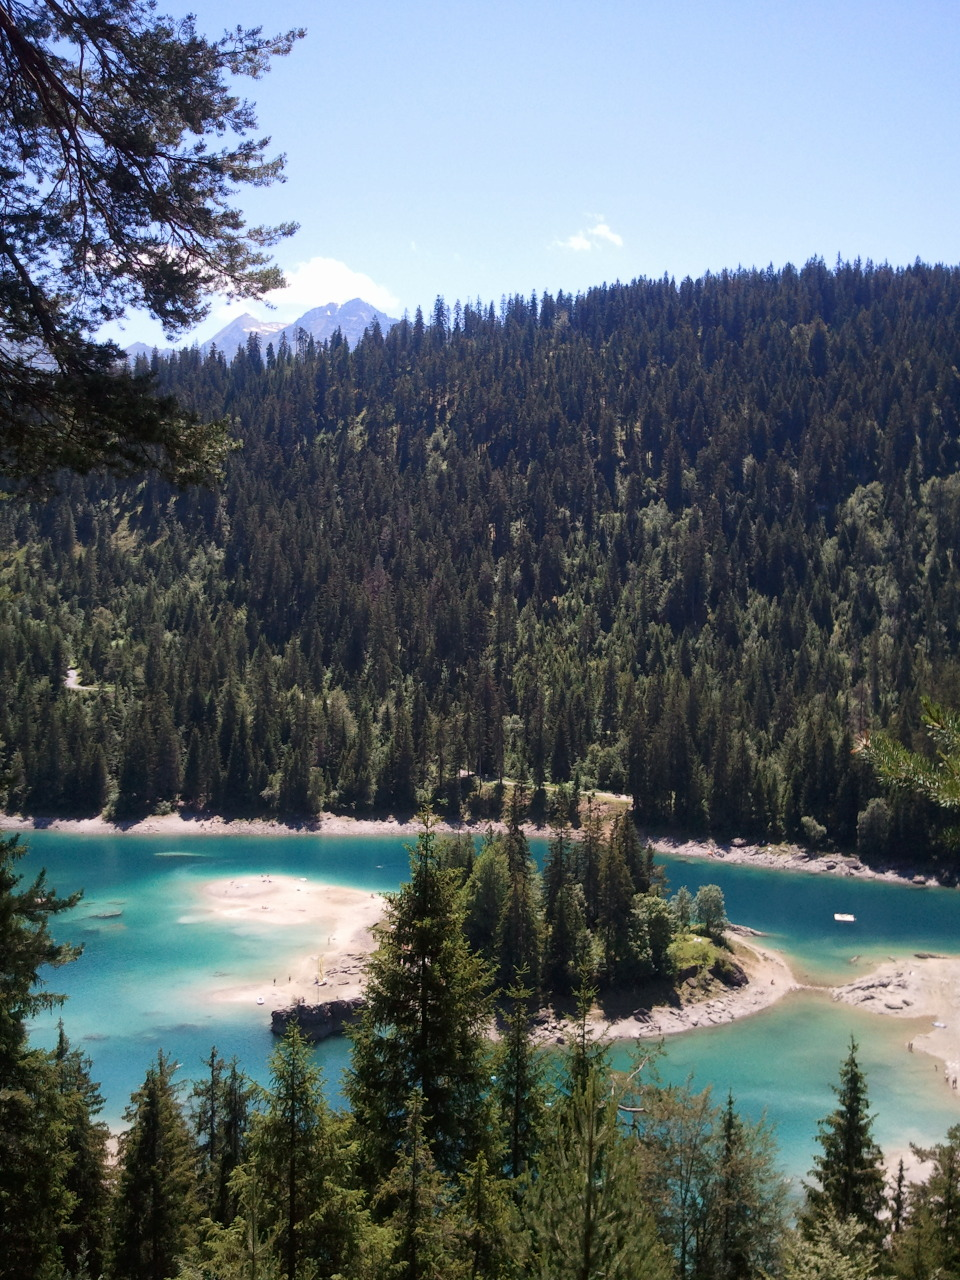
\includegraphics[width=0.4\textwidth, height=5cm, keepaspectratio]{../Bilder/Flims/21.jpg}
    \caption{Caumasee}
  \end{centering}
\end{wrapfigure} 

Nach einer kühlen aber angenehmen Nacht versuchte die Sonne durch unsere neuen Vorhänge zu scheinen und scheiterte natürlich kläglich.
Die bestellten Gipfeli waren im Laden / Reception des Campingplatzes bereit und wurden abgeholt.
Gerade als die ersten Kaffeedämpfe meine kleine Bialetti Kaffeemaschine verliessen, beschloss die Gas Buddel leer zu sein.
Kein einziger Tropfen fand den Weg nach oben durch das Kaffeepulver.
Auf an den Caumasee und die Wärme geniessen.
Meine anfänglich sehr optimistische Ankündigung zur Insel hinaus zu schwimmen wurde durch den ersten Kontakt mit dem 18°C (warmen) Wasser korrigiert.
Chantal stürzte sich natürlich todesmutig in die eisigen Fluten und schien es sogar zu geniessen.
Mit roter Nase und verbrannten Füssen machten wir uns mit den Bikes wieder an den beschwerlichen Aufstieg, damit wir dieses eine Mal auch sicher nicht zu spät sind um uns das Rennen anzuschauen.
Doch auch dieses Mal blieb uns der Erfolg vergönnt und wir sahen einmal mehr nur noch die letzten Streckenposten, die das Material zurück zum Sportcenter brachten.
Da wir schon einen Grossteil aufgeräumt hatten und so noch etwas Zeit hatten, beschlossen wir einen unbedeutenden Umweg zu machen, um noch ein paar Blicke in die Rheinschlucht zu erhaschen.
Diese konnte sich ja schlecht aus dem Staub machen.
Google Maps, zeigte sich wieder einmal von seiner schönsten Seite und Lotste uns über Wege, die normalerweise eher als Pfade bezeichnet werden würden.
Unser tapferer Bus quälte sich problemlos durch den Staub und den schier unpassierbare Gegenverkehr.
Schlussendlich wurden wir jedoch mit wunderschönen Aus und Einblicken in die Rheinschlucht belohnt.
Den Weg zurück nach Dättwil verlief ziemlich Ereignislos und mit nur geringem Stau.

\subsection{Rückfahrt}
Nach zwei wunderschönen Tagen waren wir zurück mit vielen wunderschönen Eindrücken und Erlebnisse.
Unser Ausbau hat sich grösstenteils bewährt und wir wissen nun, dass wir auf jedenfalls auf dem richtigen Weg sind.

Die Gegend um Flims haben wir sicher nichtcaumaseedas letzte Mal besucht und auch der kleine aber feine Campingplatz bleibt uns in bester Erinnerung.

\begin{figure}[hb]
    \centering
    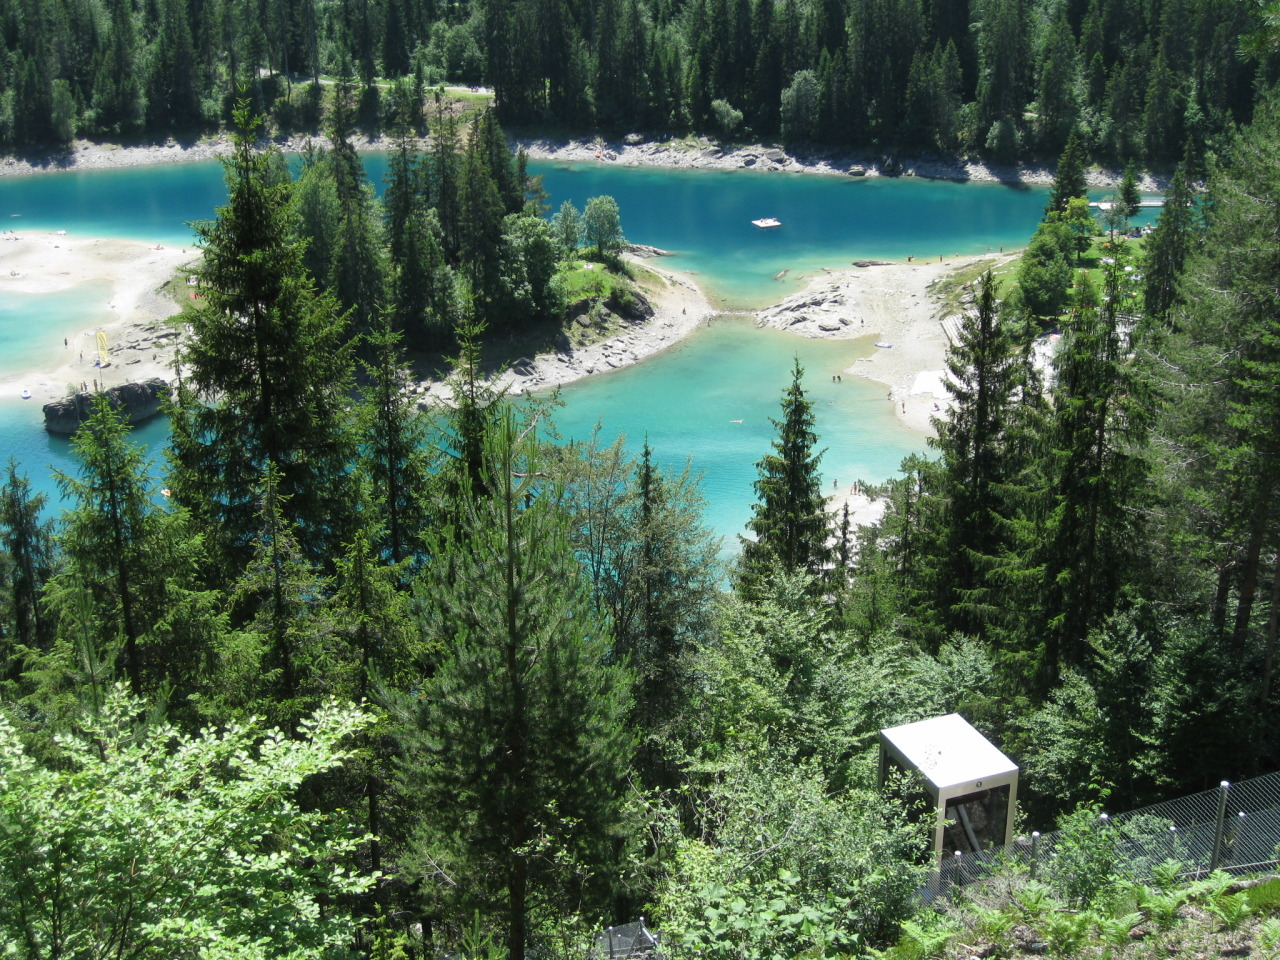
\includegraphics[width=\textwidth]{../Bilder/Flims/22.jpg}
    \caption{Caumasee}
    \label{img:Flims1}
\end{figure}

\newpage
\section{Moon and Stars 2011}
\subsection{Vorbereitungen 13.07.2011}
Da ich am Abend eingeladen war,  bei einer Elektroinstallation zu helfen, ergriff ich gleich die Chance und holte den Bus, um am Freitag p�nktlich an das Geburtstags-Essen zu kommen.

\subsection{Freitag 15.07.2011}
Eigentlich wollte im den Nachmittag frei nehmen, um zu packen und den Bus zu beladen.
Jedoch waren da noch zwei Testfl�ge im Weg und so wurde es nach 17 Uhr bis ich die Flugzeugwerke in Stans verlassen konnte.
Gerade so schaffte ich es zum Nachtessen in der Seerose.
Nach einem feinen Nachtessen musste also noch unser ganzer Karsumpel eingepackt werden.
Die spontan eintretende M�digkeit machte das unterfangen nicht gerade leichter und auch der Wetterbericht verhiess nichts Gutes f�r die kommenden
Tage.
Diese Vorhersage bedeutete, dass eher noch mehr Material den Weg in den Bus finden musste.

\subsection{Samstag 16.07.2011}
\begin{wrapfigure}{R}{0.45\textwidth} 
  \begin{centering}
    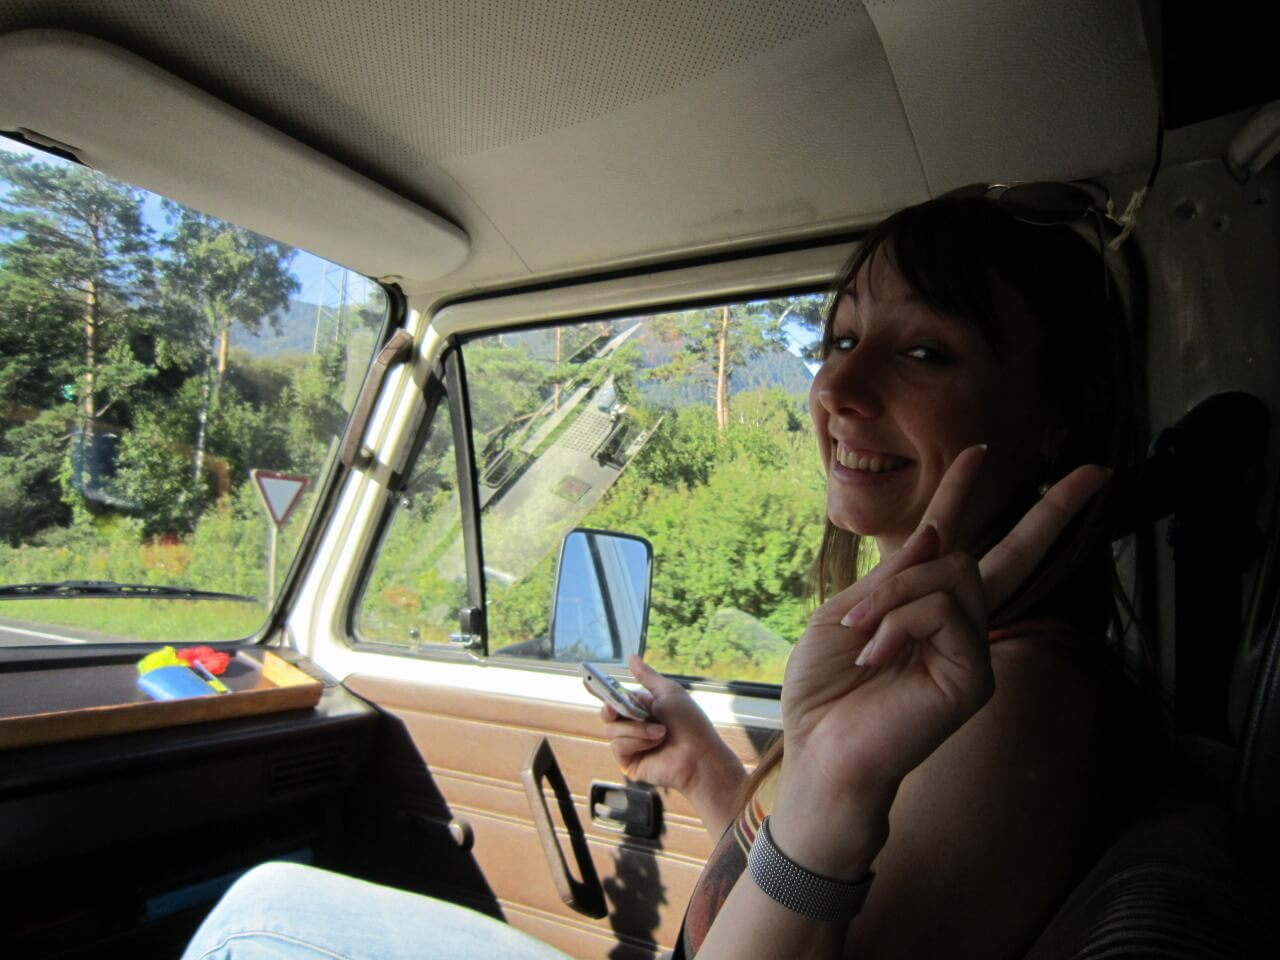
\includegraphics[width=0.4\textwidth, height=5cm, keepaspectratio]{../Bilder/Locarno/3.jpg}
    \caption{Ab in den S�den}
  \end{centering}
\end{wrapfigure} 

Nach einer viel zu kurzen Nacht hiess es um kurz nach 5 Uhr ab auf die F�sse.
Mir fiel es nicht gerade schwer aufzustehen, da mein Magen das klare Kommando zum entleeren seiner selbst gegeben hat.
Ich bekam die volle Wucht des gef�rchteten Nachbrandes nach dem Genuss von scharfem Essen zu sp�ren.
Nach kurzer Zeit war es relativ ruhig im Bus und alle Beifahrer schlummerten und tr�umten von Sonne, Strand und Jack Johnson.
Kaum auf die Westumfahrung aufgefahren, machte uns eine grosse Tafel darauf aufmerksam,
unsere geplante Route durch den Gotthard zu verlassen und dem San Bernadino einen Besuch abzustatten.
Nach kurzer Recherche konnte uns das Argument von fast zwei Stunden Wartezeit �berzeugen und so ging es Richtung Chur dem San Bernadino entgegen.
Der obligate Halt im Heidiland verbrachten wir mit Diskussionen �ber die WC- Bons und nat�rlich kam gerade vor uns ein Car mit einer ganzen Ladung Blumenkohl an, welche erbarmungslos alle verf�gbaren Kassen verstopften.
W�hrend der weiteren Fahrt gen
S�den verpasste Chantal so ziemlich alle sch�nen Sujet beim Studium der Bedienungsanleitung ihrer neuen Kamera.
Die Ersatzbank war eh schon l�nger am d�sen und nickte im Takt der Fahrbahnunebenheiten.
Im gelobten Tessin angekommen, forderte uns das Navi mit einer Strasse von 1.5 Fahrbahnbreiten heraus.
Schon bald kamen wir dann auf dem Camping Delta an.
Die zuerst unfreundliche Dame am Schalter bestand darauf, dass ich ihr pers�nlich meinen Ausweis unter ihre Nase halte.
Als Michel und ich vor ihrem H�uschen auftauchten, verbesserte sich ihre Laune schlagartig.
Der Platz war schnell gefunden und unsere zwei Untermieter machten sich sofort daran ihr neues Zuhause aufzustellen.
Kaum stand das mobile Heim war auch schon der Teufel los und es regnete wie es nur im Tessin seichen kann.
Gl�cklicherweise besserte sich das Wetter wieder und der kleinen Ausfahrt ins Maggia Tal stand nichts mehr im Weg.
Je weiter wir dem Tal folgten, desto schlechter wurde das Wetter.
So fanden wir uns bald
darauf wieder auf dem Weg zur�ck nach Locarno Richtung besseres Wetter.
Ein lauschiges Pl�tzchen an der Maggia war auch schnell gefunden.
Michel und ich unternahmen eine ausgedehnte Erkundungstour und h�pften gazellenartig geschickt von Stein zu Stein um dem kalten Wasser zu entkommen.
Dank eines netten Nachbarn entstand ein Gruppenfoto.
Es wird gemunkelt, dass gewisse Personen nach diesem Foto ihren Psychologen aufsuchen m�ssen um die schrecklichen Bilder aus ihrem Kopf zu verbannen.
Der nette Fotograf parkte sein nur durch feine, hautenge Badehosen bedecktes Geh�nge kniend auf einem Stein vor uns, um einen sicheren \glqq Stand\grqq{} f�r die Kameraausl�sung zu haben.
Die nachfolgende Shoppingtour im Coop geh�rt in das Kapitel: Geh nie mit Hunger einkaufen.
Der Besuch des angrenzenden Bistros konnte man getrost auf die selbe Ebene wie ein Besuch des Bahnhof Buvette am Samstag Morgen stellen.
Lauter merkw�rdige Gestalten mit teils argen modischen Missgeschicken bev�lkerten diesen Ort.
Zur�ck auf dem Campingplatz steigerten wir uns nach einer kurzen Verschnaufpause w�hrend dem Ap�ro in einen wahren Speedmington Rausch.
Da die Flasche Prossecco durchaus Anklang bei der weiblichen Begleitung fand, stieg auch der L�rmpegel und schon bald war dir Umgebung Menschenleer.
Nach einem l�ngeren Ballwechsel war es an der Zeit sich im See abzuk�hlen.
Hart wie M�nner sind, konnten uns auch die vorbeitreibenden Eisberge nicht erschrecken und wir tauchten gen�sslich im Lago.
Fabienne kr�nte das Nachtessen mit ihrer pers�nlichen Interpretation einer Rahmsauce.
Das Bier verschwand schneller als es aus der K�hlbox getragen werde konnte und so begruben wir schon bald die Idee noch nach Locarno zu \glqq wandern\grqq{}.
Das Bett war zu diesem Zeitpunkt eine viel zu gute Alternative.

\begin{figure}[H]
   \centering
      %\sDas Keyboard 4 Professional	ubfloat[CAPTION]{BILDERCODE}\qquad
   \subfloat{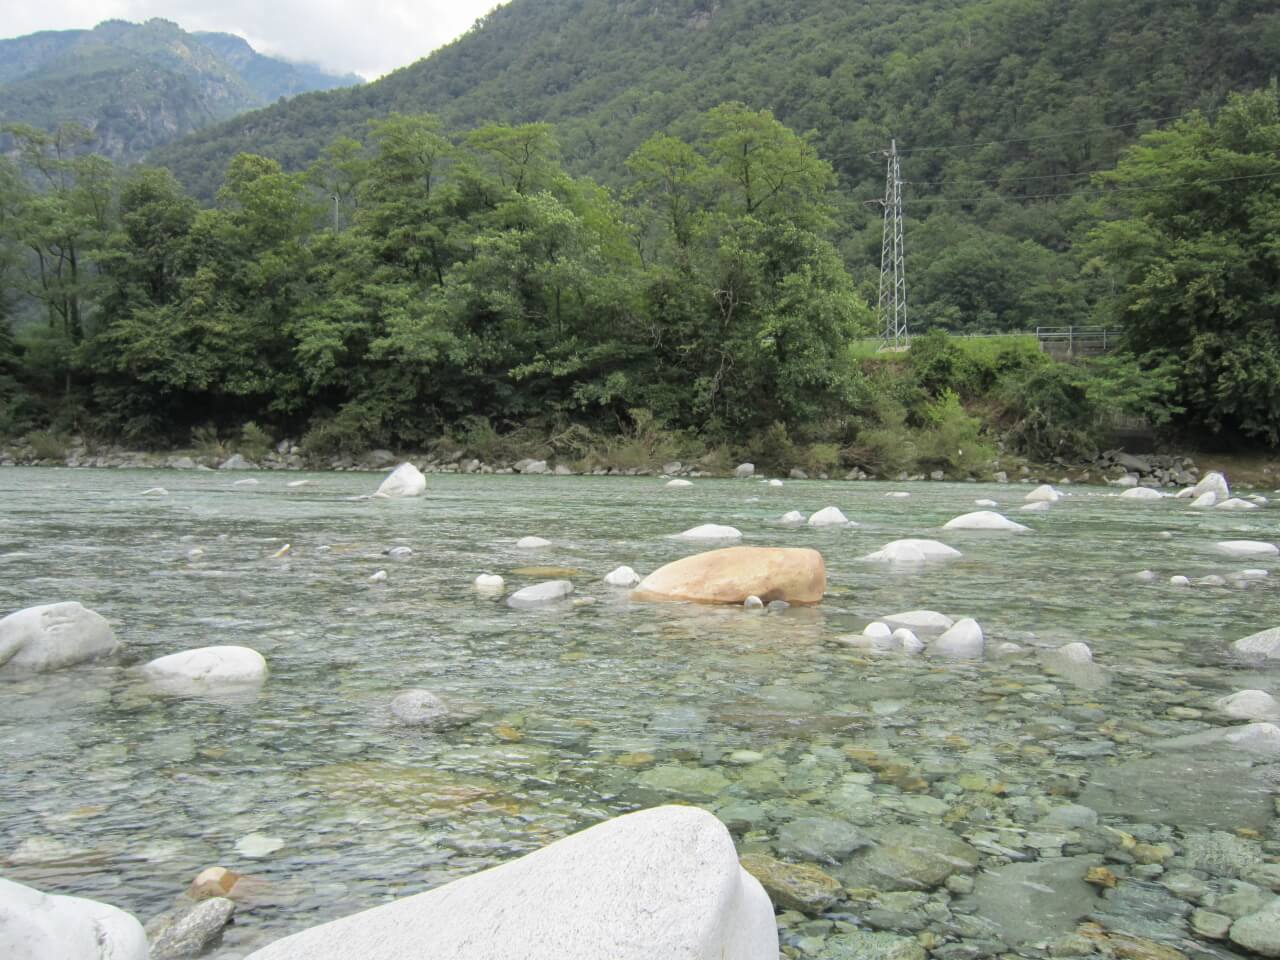
\includegraphics [width=0.3\textwidth]{../Bilder/Locarno/9.jpg}}\quad
   \subfloat{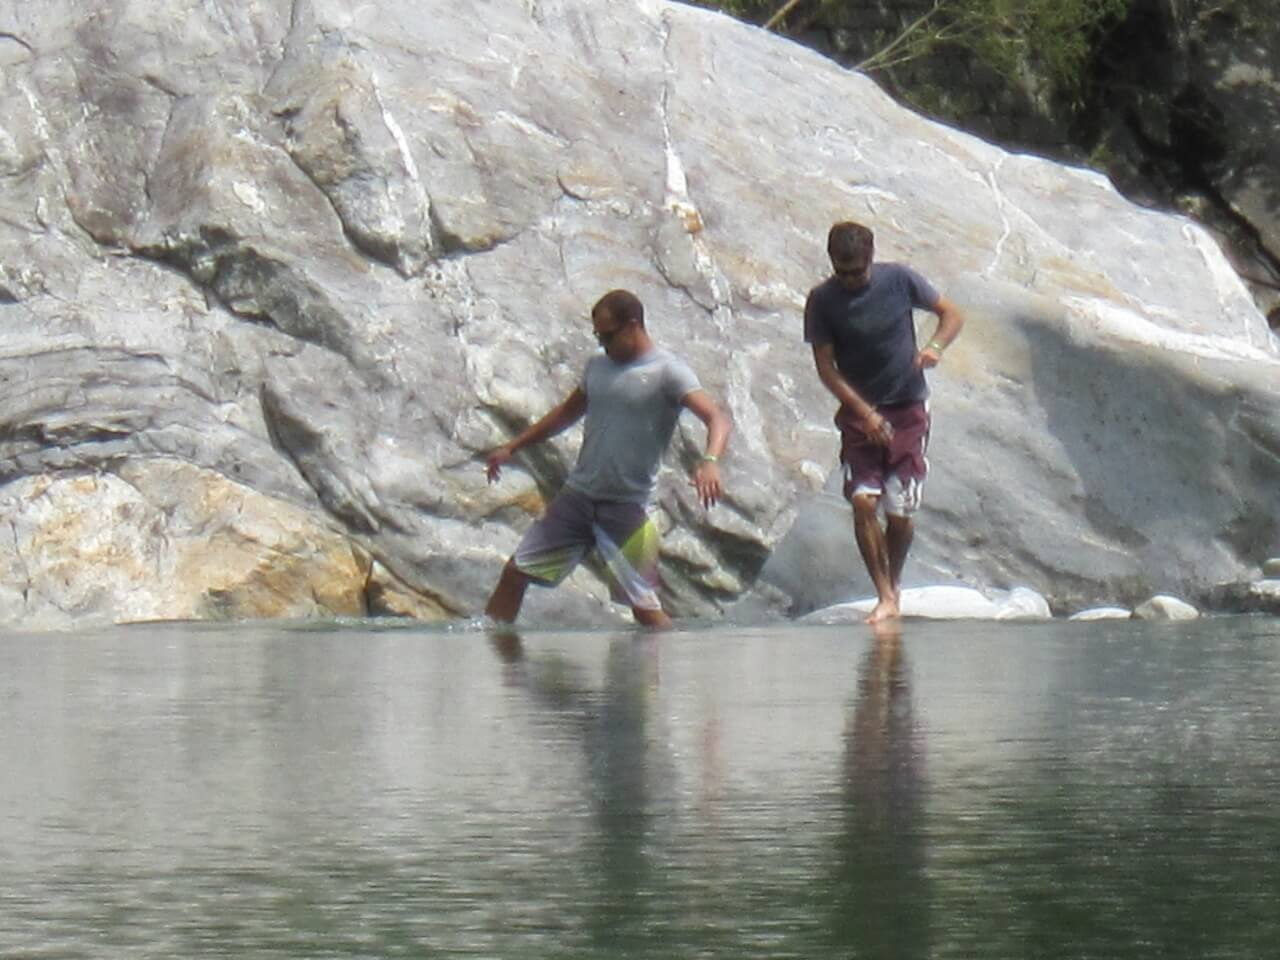
\includegraphics [width=0.3\textwidth]{../Bilder/Locarno/11.jpg}}\quad
   \subfloat{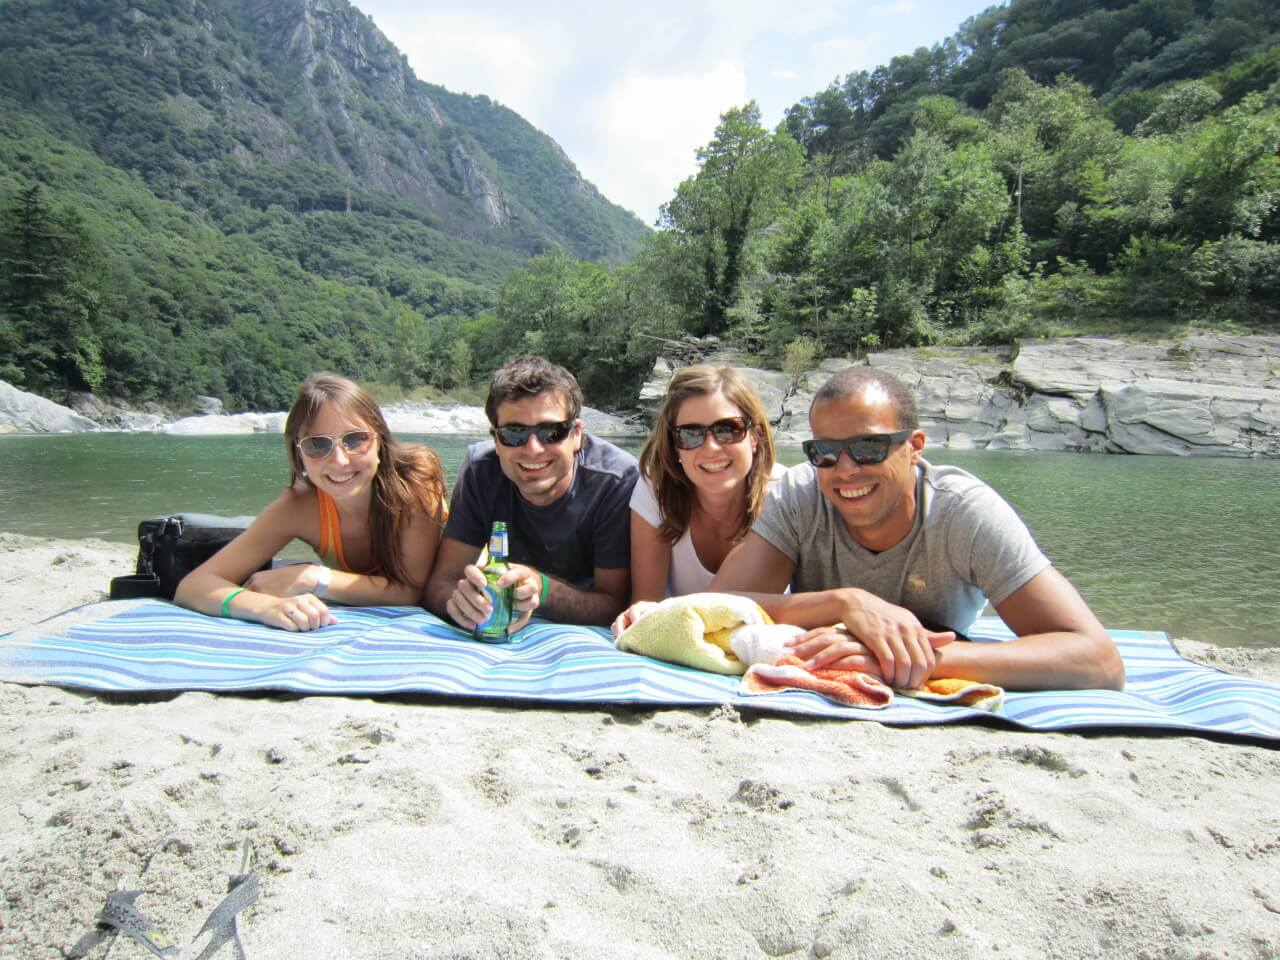
\includegraphics [width=0.3\textwidth]{../Bilder/Locarno/15.jpg}}\quad
   \caption[Action an der Maggia]{Action an der Maggia}
\end{figure}

\subsection{Sonntag 17.07.2011}
Das einheitliche Grau vor dem Fenster liess nichts Gutes erahnen.
Schon w�hrend der Nacht wurde alles mit reichlich Wasser begossen.
Irgendwie gelang es uns trotz allem das Fr�hst�ck im freien w�hrend einer Regenpause zu uns zu nehmen.
Nat�rlich wuchs der Wunsch nach Cannobio an den ber�hmt ber�chtigten Markt zu gehen.
Die Variante mit dem Schiff in das angrenzende Ausland zu fahren wurde nicht gerade positiv aufgenommen.
W�hrend der kurzen Fahrt �ffnete der Himmel alle Schleusen und die Fahrt glich eher einer Bootsfahrt, welche ja kurz vorher noch eher negativ bewertet wurde.
Die Kolonne welche uns Eingangs Cannobio erwartete verhiess nicht Gutes.
Der lokale Sportplatz wird am Sonntag regelm�ssig zum Parkplatz umgebaut und auch wir stellten den Bus in Mitten von anderen Schweizer Schn�ppchenj�ger ab.
Zuerst mussten Moneten organisiert werden.
Die Situation �hnelte sehr stark dem Parkplatzproblem.
Die Nachfrage �bertraf das Angebot.
W�hrend dem Anstehen bekamen wir aus dem fernen Aargau den Hinweis, dass der Markt nur bis um 13:00 Uhr ge�ffnet hat.
Es war jedoch schon nach 12:00 Uhr und diese Tatsache erh�hte den Ausstoss von Stresshormonen beim weiblichen Teil der Gruppe schlagartig.
Das Ziel der Mannschaft war der Teil des Marktes welcher Essbar ist.
W�hrend dieser Zeit stieg das Wasser auf den Strassen auf bis zu 10 cm an und die mit Schirmen bewaffneten Besucher verhakten sich bei jeder engeren Stelle des Marktes und produzierten so Staus, die sich nicht hinter dem bekannten Osterstau vor dem Gotthard verstecken musste.
Einen Platz in einem Restaurant zu finden, nachdem die Marktfahrer begonnen haben ihre St�nde abzubauen stellte sich als n�chste Herausforderung heraus.
Nach kurzem Warten, welches wir mit einem Apero verk�rzten fanden wir vier der begehrten Pl�tze und konnten gen�sslich an der wohlverdienten Pizza knabbern.
Der Weg zur�ck nach Locarno war von einem Element gepr�gt: Wasser.
Genauso wie das Wasser stieg, machten wir uns auch zusehends Sorgen �ber das Zelt auf dem Zeltplatz.
Dort angekommen bot sich uns ein trauriges Bild.
Es hat sich bereits ein massiver See um das Zelt aufgestaut.
Wir blieben zu viert im Bus und verk�rzten uns die feuchte Zeit bis zum Konzert mit einem T�ggeliturnier.
Danach  mussten wir uns m�glichst Wasserdicht verpacken und auf den Weg nach Locarno machen.
Chantal und Fabienne schlugen ein Tempo an, dem wir unm�glich folgen konnten.
Die beiden watschelten wie die Feuerwehr Richtung Konzert.
Chantal schmuggelte gekonnt ihren Knirps in das Konzertgel�nde und auch der Wettergott hatte etwas erbarmen und schloss die Schleusen f�r die n�chste Zeit.
Auf der B�hne spielten bereits the wailers und wir versuchten uns m�glichst geschickt zu positionieren.
Es misslang uns jedoch geh�rig.
Das Publikum war bunt gemischt und wir brachten es fertig uns direkt vor eine Gruppe besoffener Ostschweizer zu stellen.
Trotzdem war das darauf folgende Konzert ein voller Erfolg und auch das Wetter hielt.
Auf dem R�ckweg musste Michel dem irrsinnigen Flip-Flop Marschtempo Tribut zollen.
Sein Knie spielte nicht mehr mit.
Bald schon schliefen wir nach der Ankunft auf dem Campingplatz ein.

\begin{figure}[H]
    \centering
    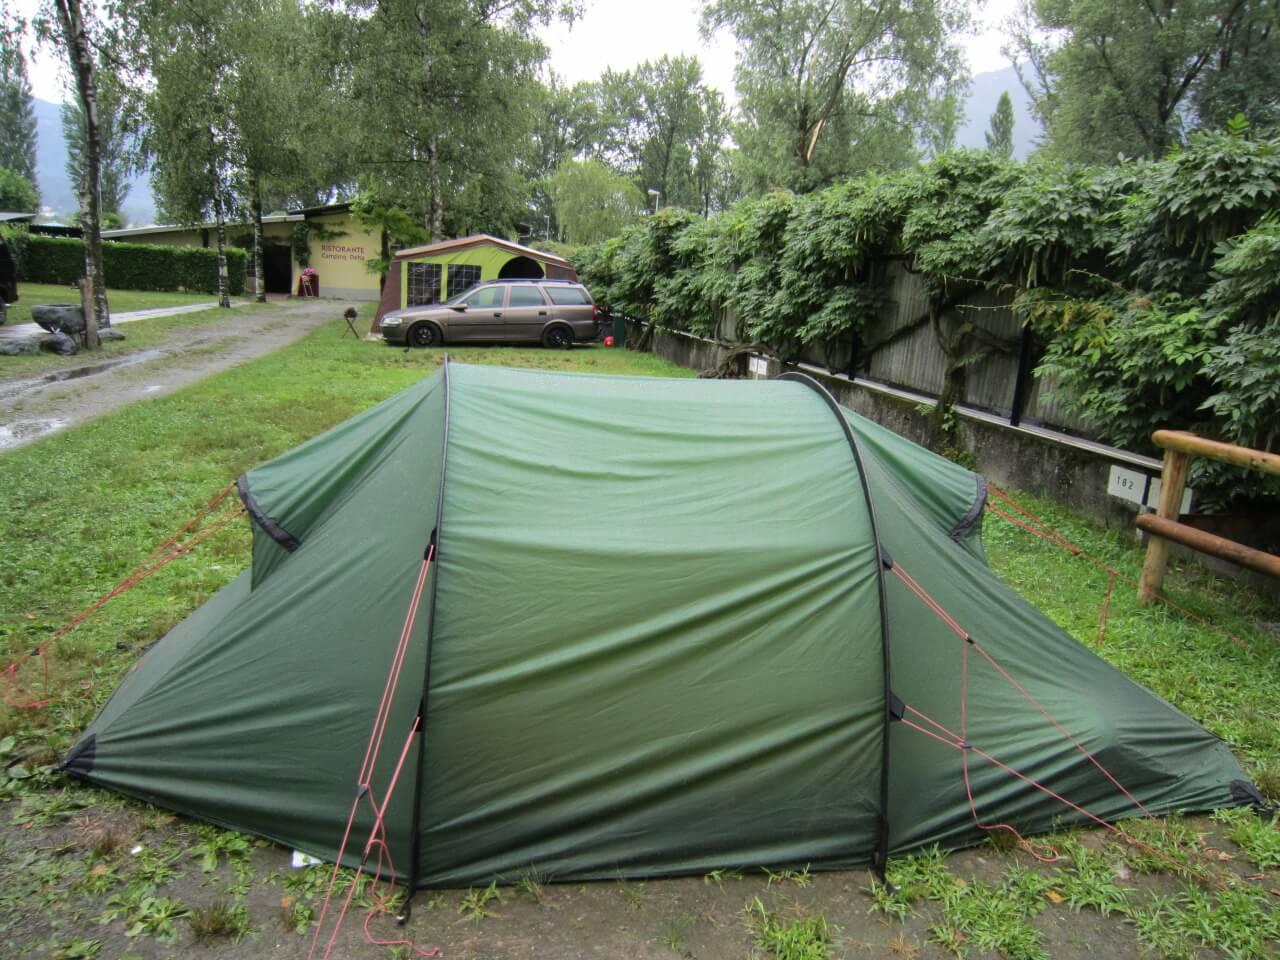
\includegraphics[width=0.6\textwidth]{../Bilder/Locarno/5.jpg}
    \caption{Wasserzelt}
    \label{img:MoonandStars}
\end{figure}

\subsection{Montag 18.07.2011}
Die Sonne blinzelt durch die neuen Vorh�nge.
So erwacht man gerne.
Eine kurze doch eher k�hle Dusche und schon wurde alles f�r das Fr�hst�ck bereit gemacht.
Nach l�ngerer Suche des Siebes f�r die Bialleti konnten wir auch einen Kaffee dazu geniessen und die Sonne trocknete das arg gebeutelte Material.
Doch schon wieder waren dunkle Wolken auf dem Weg zu uns.
So beschlossen wir m�glichst viel einzupacken und uns dann auf den Weg zur�ck ins Mittelland zu machen.
Die R�ckreise verlief absolut problemlos und die R�ckbank war ein weiteres Mal mit schnarchen besch�ftigt.
Da wir sowieso �ber Z�rich fuhren konnten wir Michel gerade noch an der Haust�re abliefern und ich konnte noch kurz beim Eglin vorbeischauen um fehlendes Elektromaterial zu besorgen.
Nach der Reinigung des Busses hiess es schon wieder sich auf die Socken nach Stans zu machen, wo am Dienstag der Ernst des Lebens weiterging.
Die kurze Reise ins Tessin und an das Moon \& Stars war ein voller Erfolg und h�tte nur durch besseres Wetter �bertroffen werden k�nnen.
Wer weiss wer n�chstes Jahr in Locarno auftreten wird? ...

\newpage
\section{Korsika 2011}
\subsection{03.09.2011 Samstag}
\begin{wrapfigure}{R}{0.45\textwidth} 
  \begin{centering}
    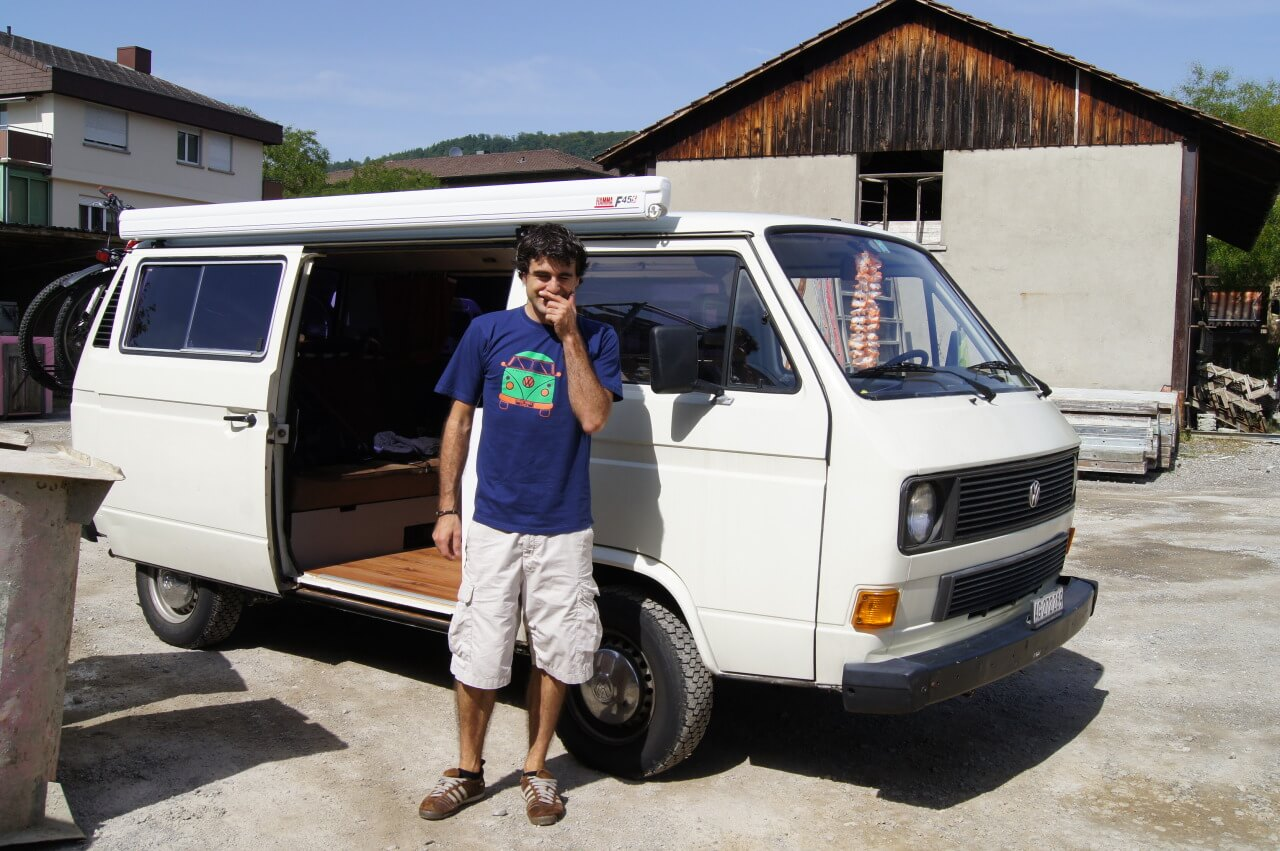
\includegraphics[width=0.4\textwidth, height=5cm, keepaspectratio]{../Bilder/Korsika/1.jpg}
    \caption{Uf gohts}
  \end{centering}
\end{wrapfigure} 
Morgenstund hat Gold im Mund... oder  au ned ;-) Am halbi 10ni simer �pe ufgstande und hend zersch mal gm�etlich zm�rgelet.
Da de Jack und de Philipp sehr gm�etlichi send, hends mer ja au chli chillig ch�ne neh;-) Scho am halbi 3 semer de startklar gsi und hend euse Jack vollglade...juhuuu, eusi erscht gross Reis met em B�sli cha afo! En Weggis hemer scho de erscht Stopp igleit und send chli an See gh�klet und hend �pis gesse und trunke.
Esch supersch�n gsi und sWetter esch traumhaft gsi.
Nach Weggis ha ich de mini Fahrk�nst welle zeige und be uf de Achsestross umed�sed...alli hend seeehr Freud a mer gha, well ich nat�rli en Speedy Consalez gsi ben:P
Vorem Gotthard, wos echli stockend witergange esch, send mini Nerve scho am Endi gsi und de Herr Bopp het m�esse witerfahre.
Mer send dor de Gotthard d�sed Richtig Italia...und sWetter esch emmer besser worde...chum send mer es Tessin cho hets afo seiche; dasch eus zemli bekannt vorcho.
E de erschte Rastst�tt em Tessin hets zNacht ge und zwar zwoi sehr chlini Portione Lasagne und Tortellini.
Meteme volle Mage und eme halbe Swimmingpool e eusem B�sli hemer die italienisch Grenze souver�n �berquert.
Zemli lang semer uf donkle, met Grillesound umgebni Strasse umekurvt bes mer denn dAutobahn gfonde hend.
Um di 10ni hemer de gfonde mer send f�r h�t gnueg uemd�st und send e Stond vor Genua ufe Rastst�tt go �bernachte.
Ruckzuckzackzack hemer euses Bettli parat gha und hend eus ed Decki ch�ne imulme.
dNacht esch echli unruhig gsi, neb de velle Autos wo cho und gange send, hend es paar obercooli Gangster gmeint sie m�sset ihri Mega-Boom-Boom-Musig en aller Lutst�rki eus abspele. 

\subsection{04.09.2011 Sonntag}
\begin{wrapfigure}{L}{0.45\textwidth} 
  \begin{centering}
    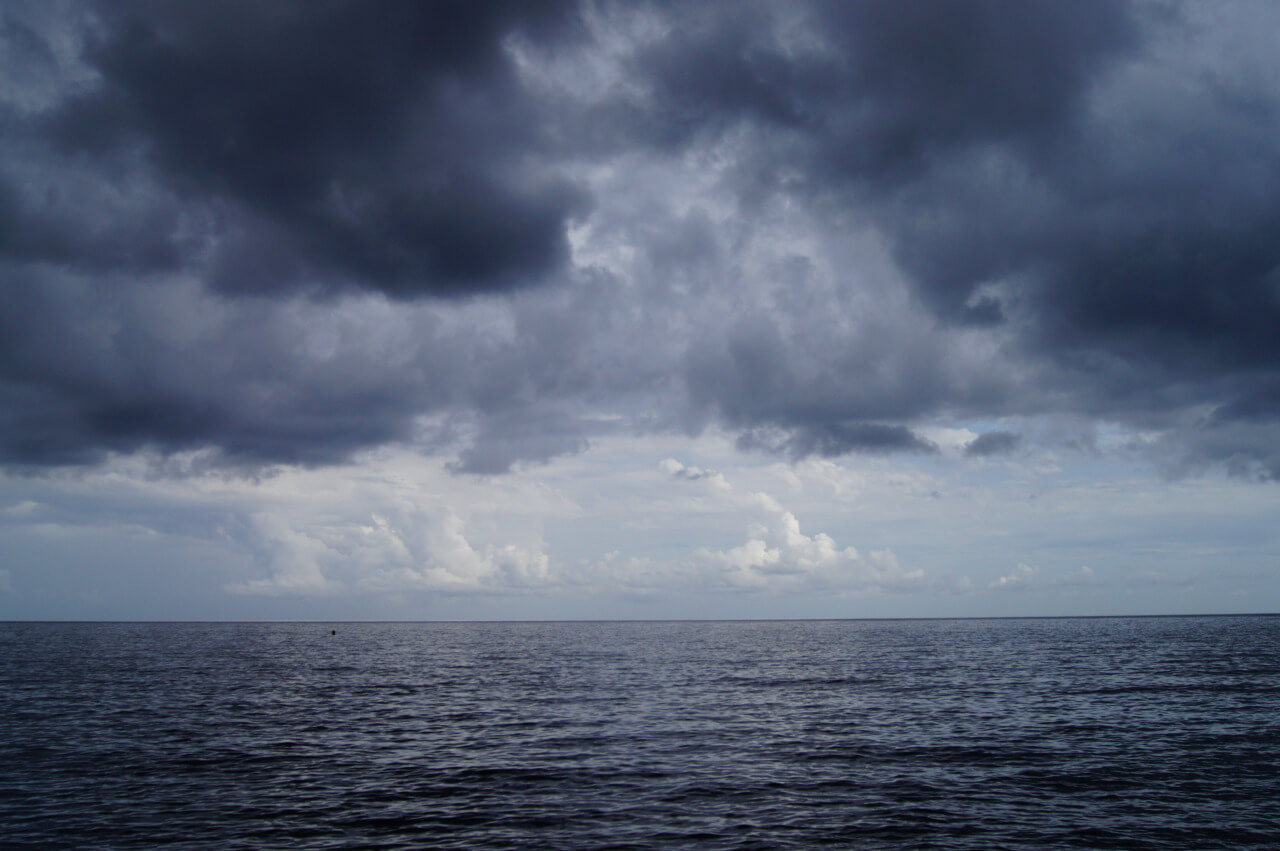
\includegraphics[width=0.4\textwidth, height=5cm, keepaspectratio]{../Bilder/Korsika/3.jpg}
    \caption{Nasser Empfang}
  \end{centering}
\end{wrapfigure} 
H�t esch fertig gsi met der Gem�tlichkeit...
versuchs mal mit Gem�tlichkeit, mit Ruhe und Gem�tlichkeit ;) scho am halb 6i semer ufgstande, hend gschnell zm�rgelet und send de schnell uf Genua d�set.
De Steff und de Jack het freud gha de kurveriche Autobahn.
Ich ha schochli Angst gha, dass mer eusi F�hri verpasset, well ufem Ticket staht, dass mer 90min vor Abfahrt scho muess ischiffe...
aber mer send p�nktlich, vellecht fasch zu p�nkltich f�r Italiener, be euse Moby Wonder acho und setzted jetzt grad ufem Deck und gn�ssed die sch�n Ussecht und dRegetr�pfli und de Wind ;) Aber siehe da dSonne esch de doch na v�recho und mer hend nachli ch�ne s�nnele e eusne Liegest�ehl.
Pl�tzlich hemer e chlini Insle und Elba ersp�ht und schlussendlich au Korsika...Korsika we are coming:) 
Met euse chline F�hri semer en Hafe vo Bastia man�vriert.
Trotz emene m�ehsame Alarmsignal esch alles guet gange und euse Jack esch gsond und ufem korsische Festland acho.
Mer send geg de Strom en Norde ufegfahre Richtig Cap Corse.
En Erbalunga hemer euse erscht Stopp gmacht und send dor die supersch�ne Altstadt bis zum Hafe gschlenderet.
Vo allem M�gliche hemer m�esse es F�teli mache ;)... alti gelb-orangi-toskanisch-aghuchti H�sli, romantischi engli G�ssli und vell herzigi Kaffis und Restaurants.
Aber leider hend eus dRegetr�pfli oder besser gseit riesigi Regetropfe bis nach Korsika verfolgt...wo mer am Hafe unde gsi send hets afo Tr�pfelet.
Gli hets afo Seiche und er send zum Jack zruggsecklet.
Denn eschs ersch recht losgange, de Petrus hets guet met eus gmeint, es esch emmer meh cho regne bis euse Jack eme Boot gliche het....
be mer hets sogar inegsprudlet!! Aber dor die superbreite und guet preparierte Strosse esch da ja ke Problem gsi.
Eigentli hemer welle en Macciagio �bernachte, aber da eusi Sicht ja biizli igschr�nkt gsi esch, hemer de Campingplatz verpasst.
Mer send tapfer witergfahre und send de ad Westk�ste cho...
ah ja da eschs Wetter ja vell besser gsi;) Jetzt semer au na fasch devogfloge! Aber damol hemer dAbzwigig f�r de Campingplatz en Centuri-Port ned verpasst und send das schmale Wegli bes zum Meer abekurvt.
De Campingplatz esch u herzig gsi, klein aber oho.
Mer hend eusi super Usr�stig met Store nat�rli ufbaut, send go dusche und hend eus uf de Weg nacheme Restaurant gmacht...
leider ned erfolgrich.
Dev�r hemer en wondersch�ne Sonneuntergang am Hafe unde ch�ne gn�sse.
Uf de Suechi nach Esse semer weder zo eusem Camping ufegloffe und damal hemer Gl�ck gha....
hmmm ufere chline Terrasse hemer fein gschlemmeret...
Entercote, Calamari, Frites und e Fl�sche Wii ;) Gschlafe hemer t���f und fescht, gw�ssi Persone send grad en Ohmacht gfalle;)

\begin{figure}[hb]
    \centering
    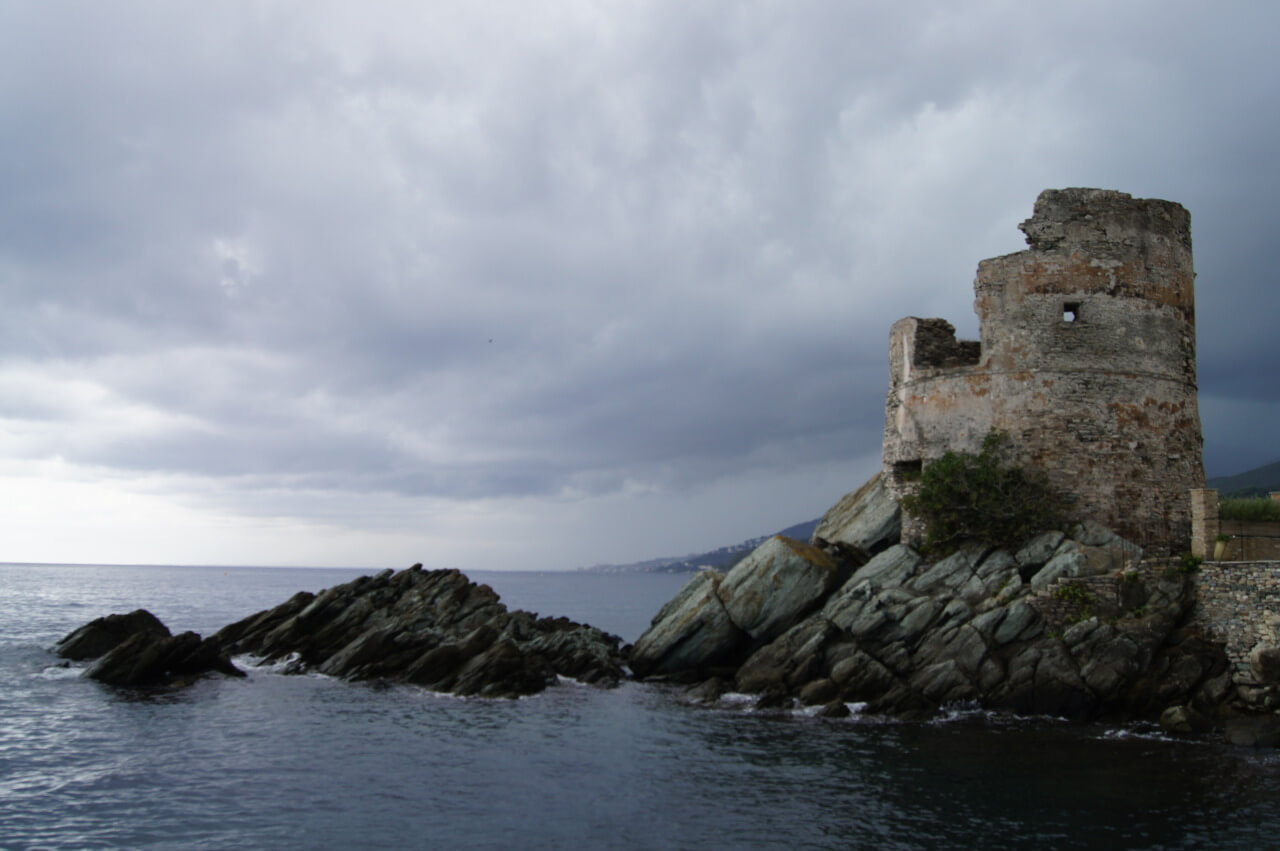
\includegraphics[width=\textwidth]{../Bilder/Korsika/4.jpg}
    \caption{Wetter het no Rum zur Verbesserig}
    \label{img:Korsika1}
\end{figure}

\pagebreak

\subsection{05.09.2011 Montag}

\begin{wrapfigure}{L}{0.45\textwidth} 
  \begin{centering}
    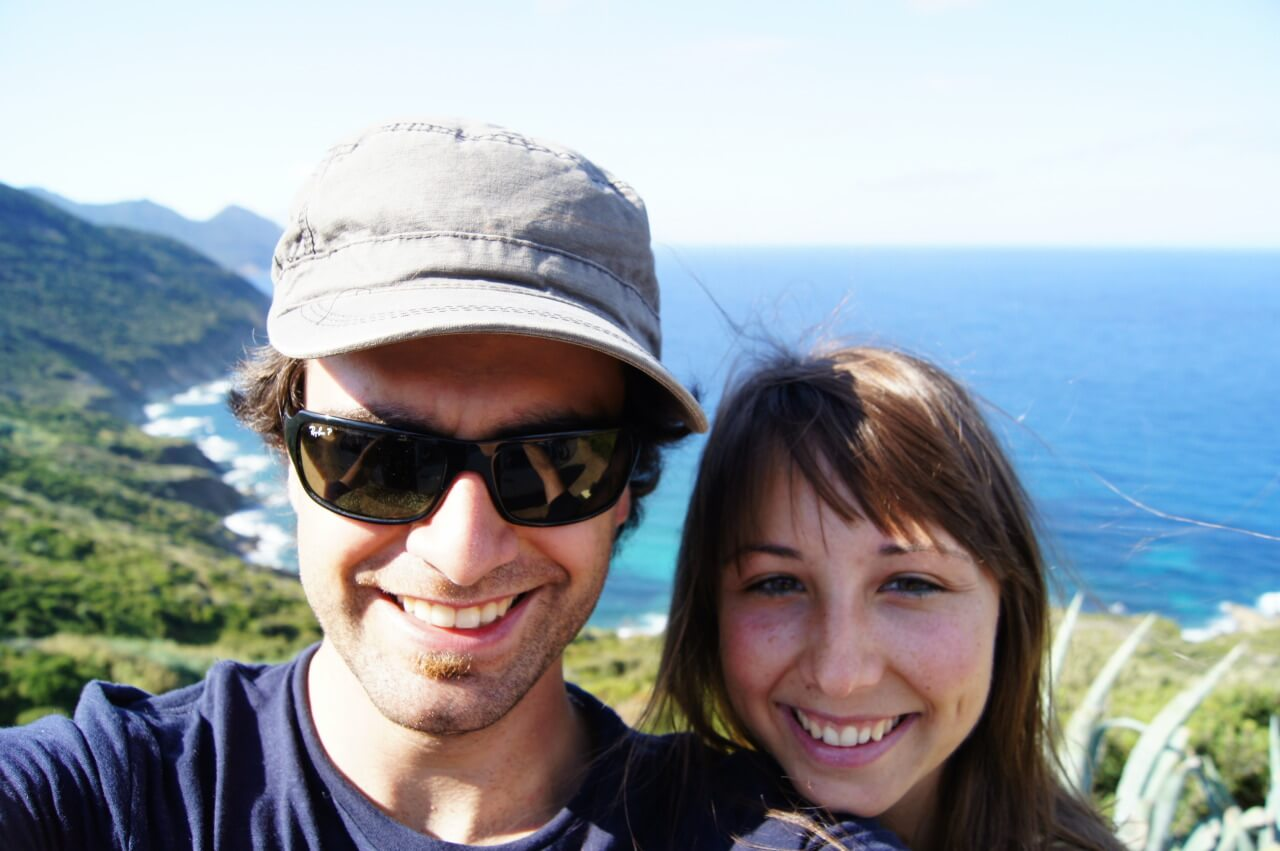
\includegraphics[width=0.4\textwidth, height=5cm, keepaspectratio]{../Bilder/Korsika/6.jpg}
    \caption{Zwei Entdecker uf Korsika}
  \end{centering}
\end{wrapfigure} 

\begin{figure}[b]
   \centering
      %\subfloat[CAPTION]{BILDERCODE}\qquad
   \subfloat{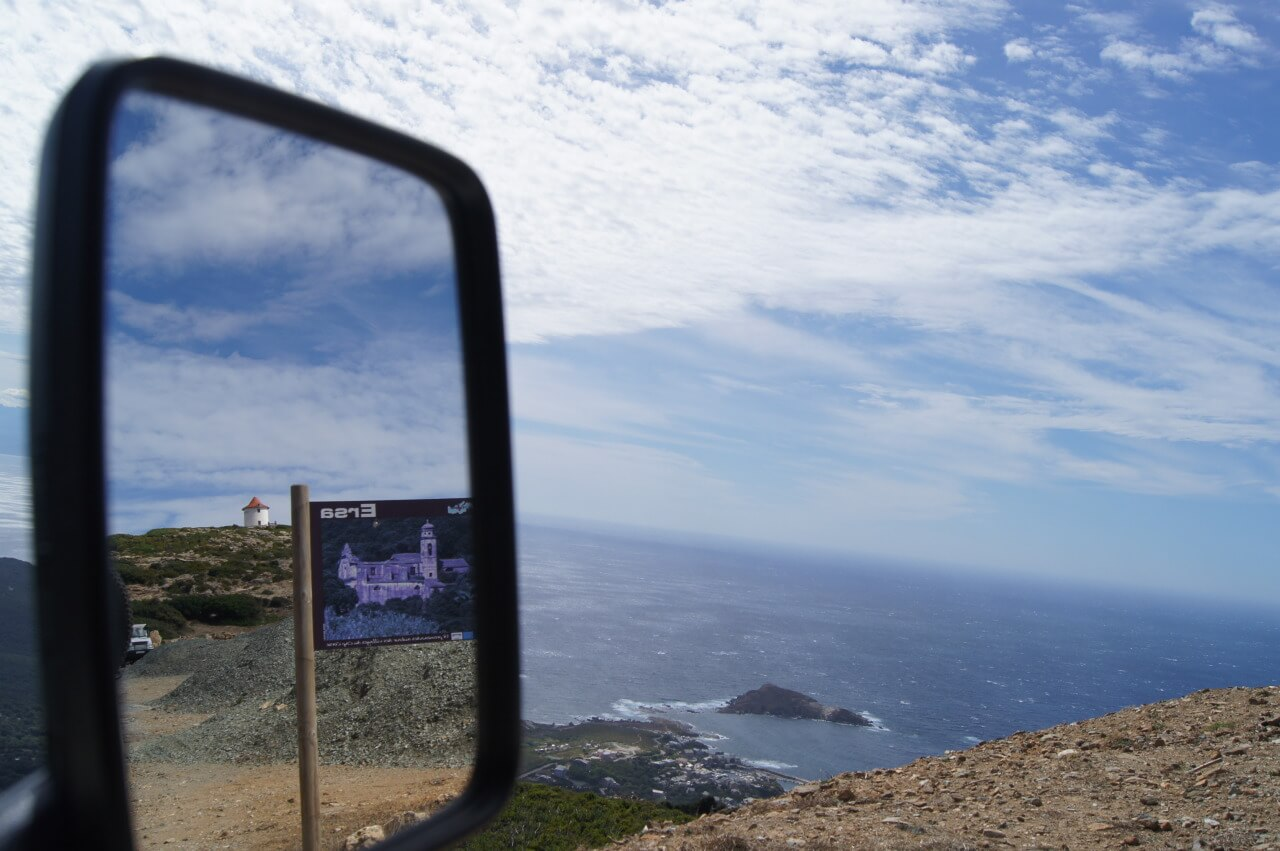
\includegraphics [width=0.3\textwidth]{../Bilder/Korsika/7.jpg}}\quad
   \subfloat{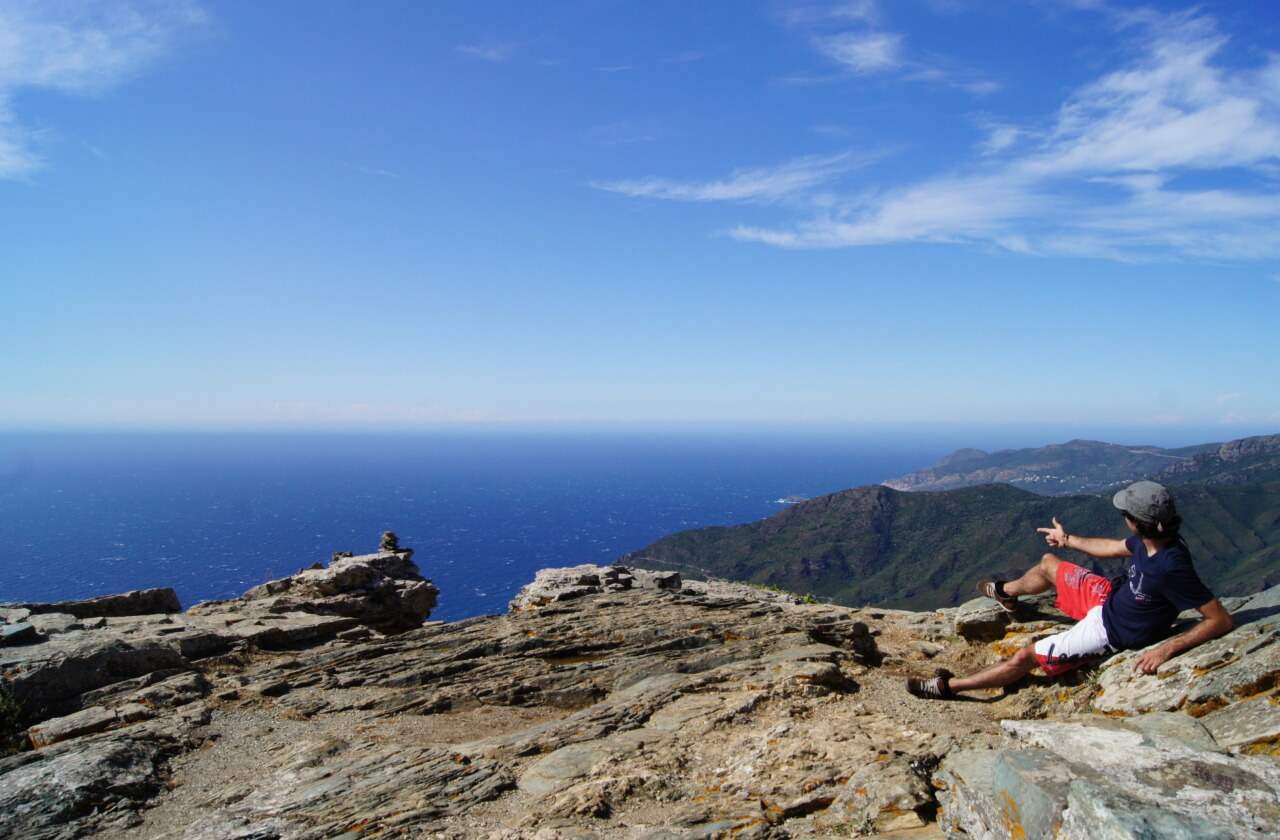
\includegraphics [width=0.3\textwidth]{../Bilder/Korsika/11.jpg}}\quad
   \subfloat{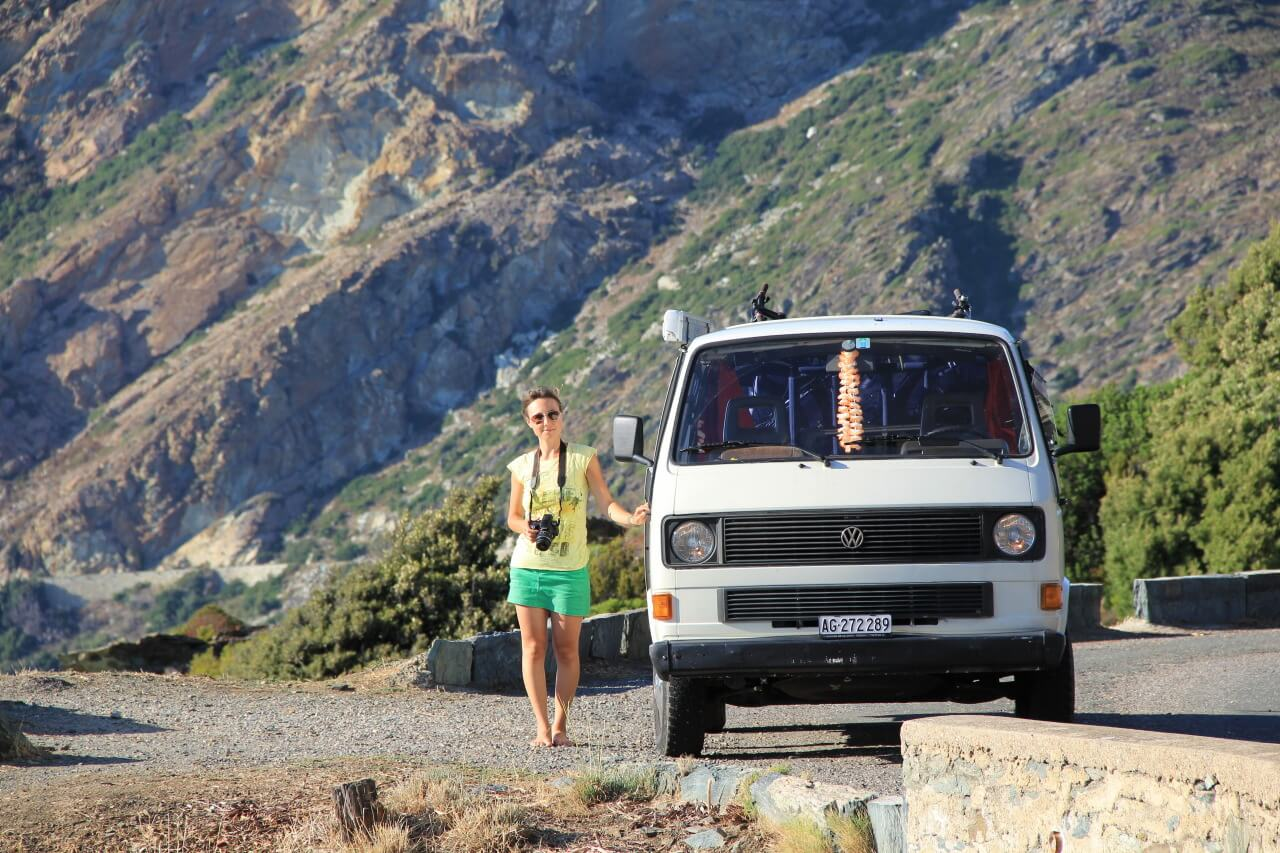
\includegraphics [width=0.3\textwidth]{../Bilder/Korsika/12.jpg}}\quad
   \caption[Korsika wie im Birlderbuech]{Korsika wie im Bilderbuech}
\end{figure}
Sonnen-Sonnen-Sonnenschein :-) In aller Frische und met eme chline Durscht semer um di 9ni ufgstande.
Zum zMorge hets suuuperfeini Croissant und en starke Kaffi ge.
Nach dem Kaffi hemer euses B�sli so schnell wie no nie ufgrumet gha und mer send back to the road an n�rdlichst Ponkt vo Korsika uf Barcaggio gfahre.
Vo Ersa het wedermal es sehr abent�rlichs Str�sslii ad K�ste gf�hrt.
De Jack und de Superdriver hend das aber super gmeisteret und mer send belohnt worde met ere wondersch�ne Bucht met de Insle Giraglia im Hintergund und emene ned allzu sch�ne Strand.
Jetzt hets gheisse: s�nnele, usruhe und vor allem B�dele...hihi...ich kenn da �per wo sich nachem B�dele gsehnt het und de nor bes zode Chn� es Wasser esch und de scho gnueg vom Bade gha het;) sWasser esch glasklar gsi und mer h�tt wit use ch�ne laufe.
Mer send de aber em Strand noche Richtig Genueseturm gloffe und hend na es chlises Restaurant gfonde, wo mer �pis trunke hend.
De semer au scho gli weder gange, well mer na es rechts Programm vor eus gha hend...nor hemer ned gw�sst das das au e Wanderig beinhaltet;) Mer send alles de K�ste entlang Richtig Pino gfahre und hend ufem Weg vell chlini herzigi Bergd�rfli atroffe.
En Pino send mer abboge f�r uf de Seneca-Ussechts-Turm.
Anstatt es winzigs Str�ssli wo mer erwartet hend, hets e sch�ni terreti Stross gha.
Scho vo witem hemer de Turm in weiter H�he obe gseh, aber dStross het de leider gar n�m so h�ch ufegf�hrt und mer hend m�esse zFuess witerga, obwohl de Turm emmer recht wit obe gsi esch.
Euse Wanderer het gmeint es g�ch 2 Stond und dOptimistin het met 30min grechnet..schlussendlich sends �pe 40 Minute gsi, wo mer steil de Berg hend m�esse ufeklettere.
Teilwis hemer w�rkli m�esse eusi Chletterk�nst uspacke und hend chli zwiflet, �b das w�rkli de rechtig Weg esch.
Dobe acho semer de met ere wooondersch�ne Ussecht belohnt worde.
dOst- und Westk�ste vom Cap Corse und die sch�n h�gelig Landschaft em Landesinnere hend mer ch�ne bestune.
Nat�rli ha ich grad es paar Panoramas m�esse sch�sse.
Nacheme usgibige Fotoshooting hemer de Abstig en Agriff gno und send de rechtig St.Florent d�set.
Nach Nonza hemer de euse Campingplatz A Stella gfonde.
Dummerwis semer ned grad direkt ad Rezeption gfahre, was dFrau Rezeptionistin alias Hilfsherif gar ned lostig gfonde het.
Sie het sich fasch n�m ch�ne erhole, het eus de aber doch na dErlaunis ge zum �bernachte.
Mer hend eus de au en super Platz direkt vorem Strand ade pole position gsicheret.
Es esch zwar chli schief gsi, aber mer hend e traumhafti Ussecht ufs wilde Meer gha.
De Sonneuntergang hemer met eme Campari und Chips uf eusne Ligist�he gnosse.
Zum Znacht hets Tomatesalat met Brot und Korsische Worscht ge.
Nachem Esse hend mer de Sternehimmel bestunt und jeglichi Sternschnuppe, Satellite und sogar Ufos ersp�ht;-) Nachem Sternegucke und Philosophiere send mer de meteme sch�ne (bizli lute) Wellerusche zfride ipfused.

\subsection{06.09.2011 Dienstag}
\begin{wrapfigure}{L}{0.45\textwidth} 
  \begin{centering}
    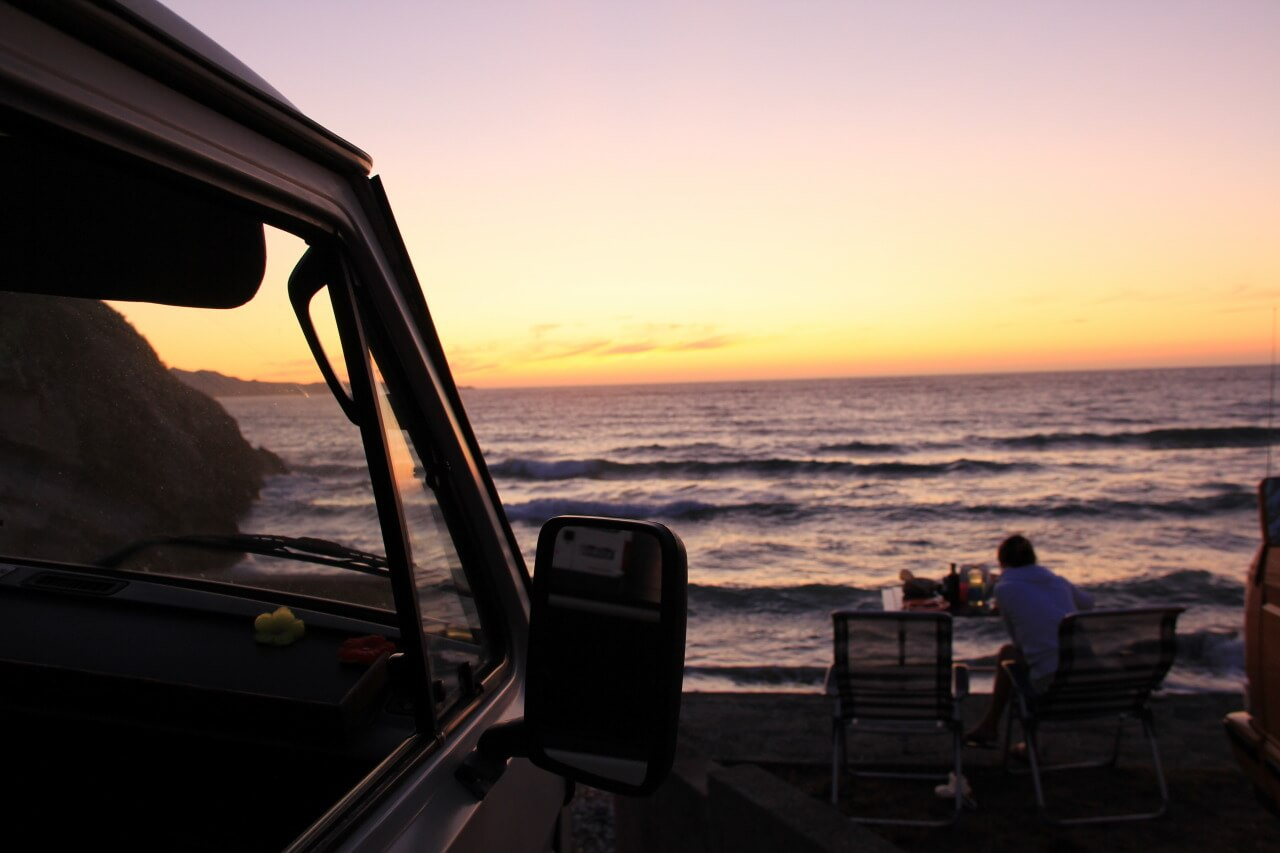
\includegraphics[width=0.4\textwidth, height=5cm, keepaspectratio]{../Bilder/Korsika/18.jpg}
    \caption{Zwei Entdecker uf Korsika}
  \end{centering}
\end{wrapfigure} 
Au ufgwacht semer metemene rusche... Wellerusche :) zM�rgelet hemer met ere geniale Ussecht uf die sch�n Bucht und send de au scho gli wederemal loszottlet.
A St.Florent semer verbigurket, well mer grad chli gschockt gsi send vo de velle L�t wos d�t gha het;) Witer Rihtig Ille Rousse hemer es paar wondersch�ni Str�nd gsichtet und send de be de vo Lozuri go b�dele.
Es het recht grossi Welle gha und de Steff het mer fasch n�m ch�ne usem Wasser bringe....ich be rechtig erstunt gsi und has chum ch�ne glaube.
Nach erschte skeptische An�cherige het er sich vode Welle n�me ch�ne trenne und esch am Strand em Welletakt ufe und abegrugelet....oh Wunder das er nacher e halbi Tonne Sand e sinere Hose gha het;-) Nachem B�dele und S�nnele semer de witer und hend en Ille Rousse en Stop gmacht.
WOW...die rote Granitfelse em t�rkisblaue Wasser hend eifach traumhaft usgseh! Mer hend en Spaziergang (met echli chlettere) zum Genuese- und L�chtturm gmacht, wo mer eifach en grandiosi Ussecht ufs St�dtli und die karibik�hnliche Buch gha hend.
Denn hemer en feini Crepes verschlunge und send nach Calvi gfahre.
Em grosse und sch�ne Campingplatz La Pinede hemer eus niederglo, hend eus fr�sch gmacht und send met em Velo ed Downtown Calvi gfahre.
Em Strand und de Isebahngleis nache semer d�set und hend en supersch�ni Ussecht uf Zitadelle vo Calvi gha.
Calvi esch en mega herzigi und touristischi Stadt met herzige G�ssli, L�deli, vellne Gelati-St�nd und sch�ne Restaurant am Hafe entlang.
Mer send enes Restaurant, wo em Reisef�hrer empfole worde esch und es esch eifach genial gsi...hmm de Steff het Teigware met Meeresfr�cht gha und ich Lachs met Ris und Gm�es. himmlisch:) Gl�cklich und met vollem Buch semer zom Camping zrugfahre und send go pfuuuse. 

\subsection{07.09.2011 Mittwoch}

sErscht mal hemer 2 N�cht uf eim Camping �bernachtet und so hemer en super gm�etliche Tag gmacht en Calvi.
Sch�n usgschlafe hemer, fein zm�rgelet und de semer met de Velos es Altst�dtli vo Calvi d�set.
Zersch semer go Zidatelle aluege, was zemli imposant gsi esch.
Neb de hoche Mure hets ganz vell sch�ni Sujets vo alte H�ser, Fenster und T�re gha zum Fotografiere, mer zwoi Hobbyfotografe hend n�m welle ufh�re met F�tele;) De Innehof vode Zidatelle esch na zemli gross gsi und es het so usgseh, wie na L�t e dene alte H�ser l�bet.
Die Zitadelle und die velle Genueset�rm send na Relikt vode genuesische Herrschaft, wo fasch es Jahrhundert �ber Korsika regiert hend.
Nach dem spannende Rundgang semer zrug zo eusem Camping hend eusi Bad- und Schnorchelsache ipackt und send an Strand.
D�t hemer gs�nnelet, b�delet und sogar gschnorchlet! Em Meer hesch mega wit use ch�ne laufe..
de Steff esch fasch de ganz Weg met de Flosse usegwatschlet;) Bem Schnorchle hemer paar sch�ni selbrigi Fisch gseh und de Steff het sogar en Tintefisch gseh, angeblich;) Ich ha n�t gseh, well de Steff so umegfuchtlet het, dass er mit sine Flosse en ganze Sandstorm veranstaltet het;) Nach dem astrengende Schnorchle semer zo eusem Jack zrug und hend fein zNacht kochet: Spaghetti met Carbonara-Sauce.
Korsische Wy hemer na kauft, aber leider esch de zemli sur gsi.
Es esch super gm�etlich gsi und mer hend gnueg Zyt gha zum die andere Camper (vor allem D�ne) met erne T�ff zbeobachte.

\begin{figure}[H]
    \centering
    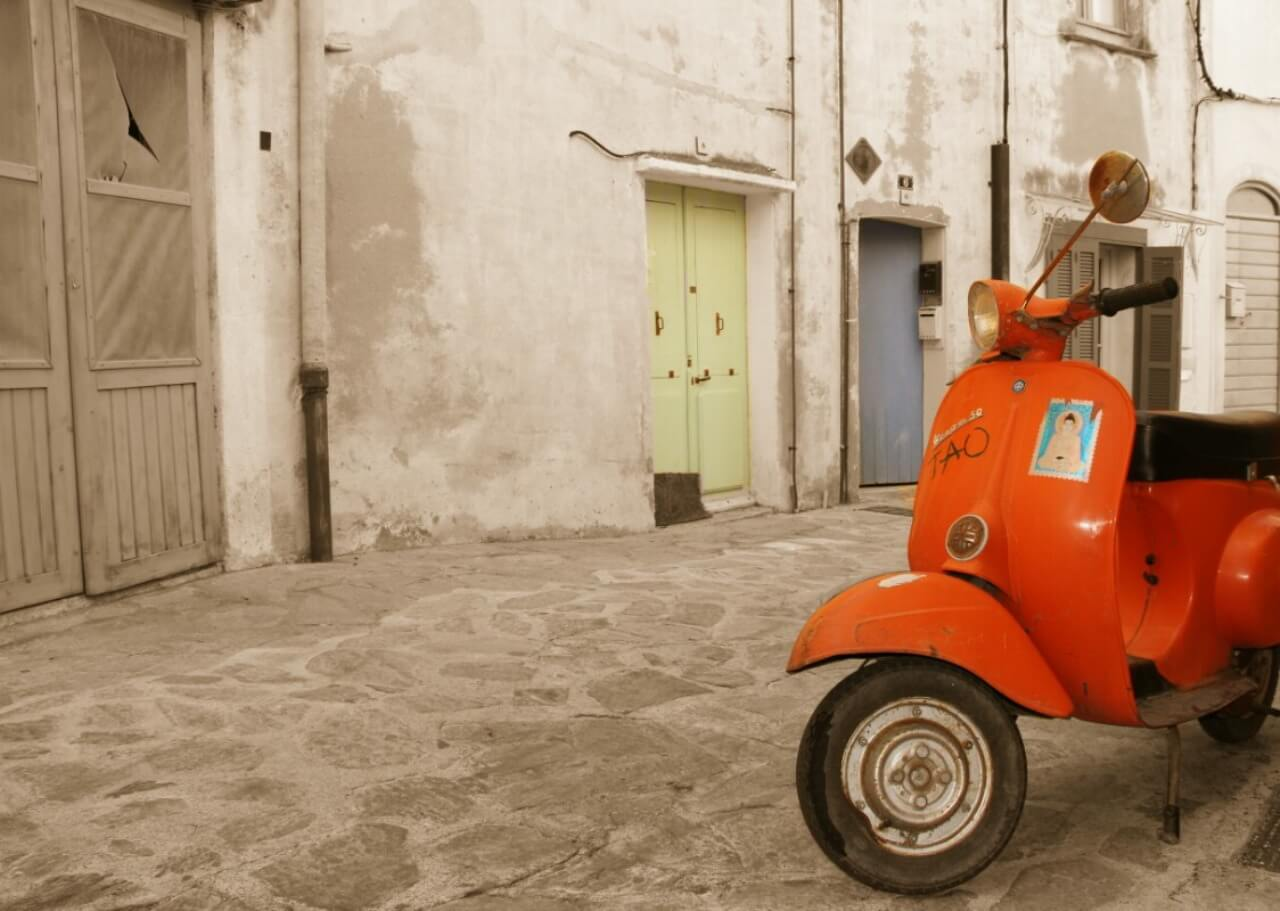
\includegraphics[width=\textwidth]{../Bilder/Korsika/25.jpg}
    \caption{Wunderbari G�ssli}
    \label{img:Korsika2}
\end{figure}
\pagebreak

\subsection{08.09.2011 Donnerstag}

\begin{wrapfigure}{L}{0.45\textwidth} 
  \begin{centering}
    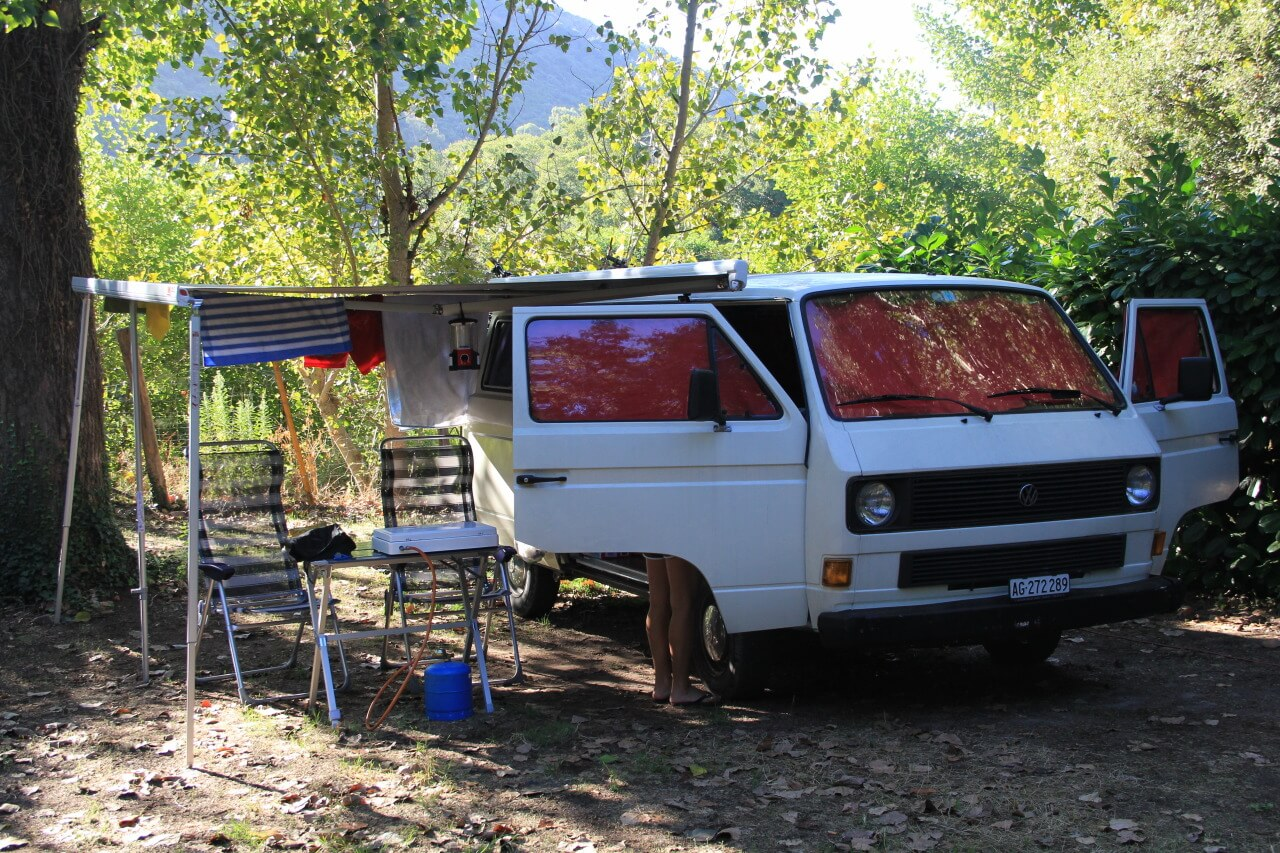
\includegraphics[width=0.4\textwidth, height=5cm, keepaspectratio]{../Bilder/Korsika/32.jpg}
    \caption{Jack in Action}
  \end{centering}
\end{wrapfigure} 

Scho am 8ti, so fr���e, semer ufgstande und hend eus los gmacht f�r en grossi Etappe.
Euses Ziel esch Porto gsi.
Ufem kurvige pass�hnliche Weg h�mer es mega sch�ns Resti anere Bucht gseh und hend denkt, d�t ch�mer sch�n zm�rgele.
Es esch au wodersch�n gsi, nor de Weg zo dem �rtli esch zemliii steinig gsi.
Aber de Jack het da super �berstande.
Met wondersch�ne Ussecht hemer en feine Kaffi gnosse.
Zrugg uf de Stross hemer witeri fantastischi Buchte erblickt und hend ufeme Ussechtsponk zm�rgelet.
Es het weder es paar F�teli ge..damol sogar na vo Libelle und Schmetterling..ah nei vo Schmetterling ned, well de Herr Bopp vo dere wilde Kreatur devogsecklet esch rings um de Jack..
hihi die andere Touriste hend zemli komisch glueget.
Aber au ich be a dem Tag unter schlechtem Insekte-Zeiche gstande.
Min Wespistech, wo ich mer am Obe vorane leider zuezoge ha het afo bisse und na dezue send mindestens 2 witeri Ficher bem Fahre es B�sli gfloge und ich ha fasch es Herzchriesi becho.
Darum be ich die ganz Fahrt zemli verchrampft em Auto ghocked.
Leider het sich au euse Superdriver chli m�esse verchrampfe, well ufem Weg nach Porto, zwoi riese Cars gmeint hend, sie m�sset die winzig schmale und kurvige K�stestr�ssli ne! So hets nat�rli en riese Stau ge und alli hend vorw�rts oder r�ckw�rts en Nischeplatz m�esse sueche.
Wo die superschlaue Cars verbi gsi send, hemer ch�ne witerfahre und send scho gli en Porto gsi.
De Golf vo Porto esch de sch�nst vo Korsika, aber leider daher au sehr touristisch.
dNatur esch wondersch�n met de knallrote Granitfelse (Em Oste hets vor allem Schiefer(Meeressedimeten)) und em t�fblaue-t�rkise Meer.
Mer send dors D�rfli spaziert, am Genueseturm verbi, well mer d�t h�t m�esse zahle und send an Kiesstrand gh�cklet.
D�t hemer leider ned ch�ne bade, well dWelle zu h�ch gsi send.
sGanze D�rfi esch eus vorcho wie em Europapark..ergendwie ned so atmosph�risch und eifach zemli k�nstlich.
Mer hend eus entschiede, gli weder ufzbreche und e chlini Wanderig em Calanche-Gebirge zmache.
Leider hets au d�t zemli vell L�t gha, aber die rot-orange Granitskulpture send schono idr�cklich gsi.
�pe e Stond em Ganze semer umegwaschlet und hend dFelsformatione, die steile Klippene und die wondersch�ne Buchte bestunt.
Denn es witer gange richtig Sagone.
Eigentli hemer en Porto welle �bernachte, aber die velle Bluemch�l-Touriste und de Weg zrug hend eus dra ghinderet.
Mer send de witer dere sch�ne, chli enge K�stestross entlang be Piana und Cargese verbi, bes nach Sargone.
D�t hemer en grosse sch�ne Camping gfonde met Restaurant, Swimming Pool und Tennisplatz....nor send mer fasch allei gsi;) Zum Znacht hemer Omelette gmacht met Banane, Zucker und Zitrone.
Es esch supi gsi...hihi...nor het �per chli welle pl�fe und het dOmelette ede Pfanne met Schwung m�esse chere...leider het sich de Henkel gl�st und die sch�n Omelette esch an Bode t�scht...da het �per sch�n dumm glueget;) Dev�r esch �per andersch vom Campari chli gflasht gsi und hets chli lostig gha;) Fig und Fertig semer es Bettli plumpst.

\pagebreak

\subsection{09.09.2011 Freitag}

\begin{wrapfigure}{R}{0.45\textwidth} 
  \begin{centering}
    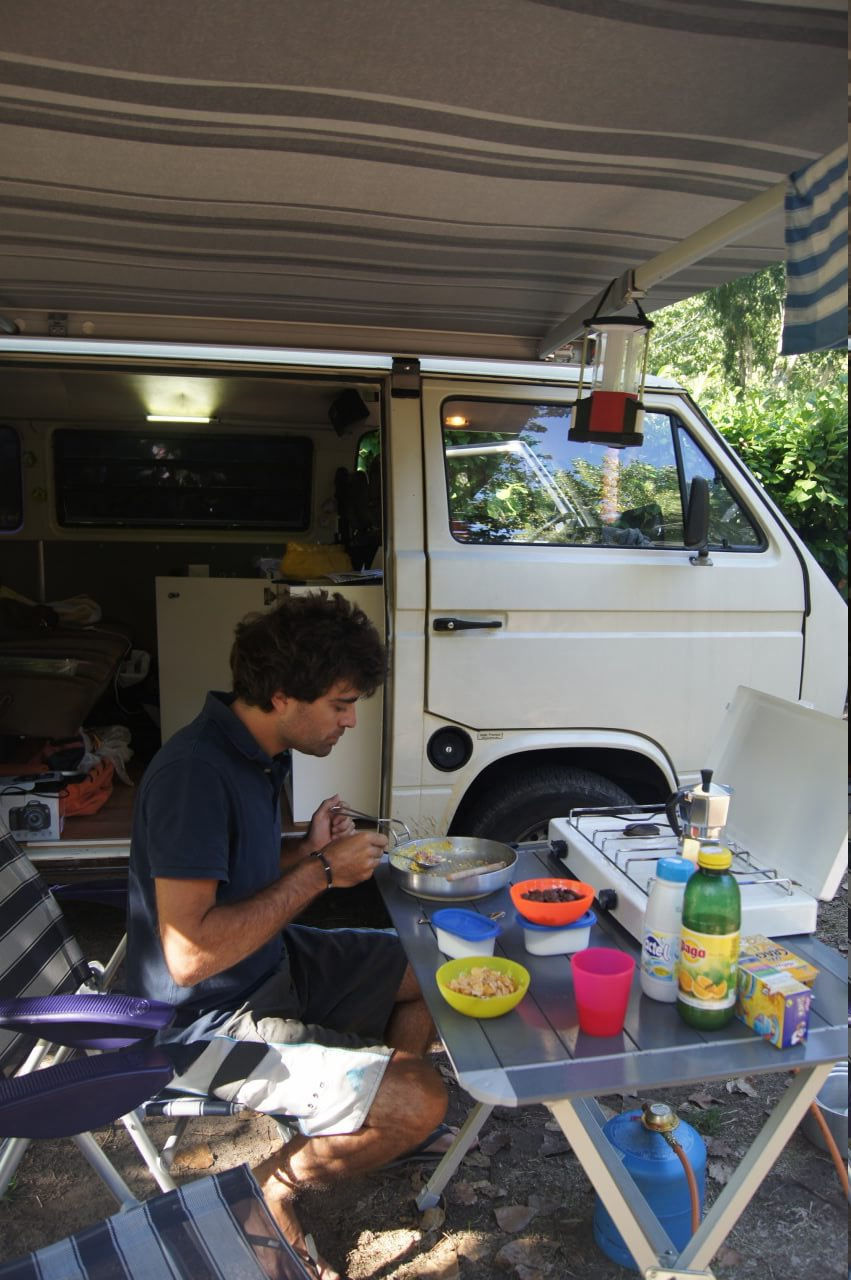
\includegraphics[width=0.4\textwidth, height=5cm, keepaspectratio]{../Bilder/Korsika/33.jpg}
    \caption{Zmorge}
  \end{centering}
\end{wrapfigure} 

H�t hemer feini M�esli und de Rescht vo eusere Omelette...R�ereier;) zum zMorge gha. 
Nachem zM�rgele hemer scho gli mal welle anen Strand go eus erhole vo de gestrige Strapaze.
En Liamone hemer en wondersch�ne Strand atroffe, wo S�ess- und Salzwasser z�mechond.
Schnell semer an Strand v�re und hend fasch n�me weg.
De Strand esch supersch�n gsi, sWasser glasklar und dWelle zemli gross.
De Pf�di het weder u Freud gha a dene Welle und esch rechtig go plantsche:) Mich hets au einisch sch�n am Strand nochezoge, was e sandigi Badhose met sich brocht het;) Speedminton hemer na versuecht zSpele, was be dem heftige Wind aber recht schwerig gsi esch.
Schliesslich hemer eus begn�egt met Fulenze, Lese und S�nnele...
die einte hends chli �bertrebe met de Sonne:-P Um di Dr� semer witer nach Propriano.
Weder �ber kurverichi Str�ssli semer de K�ste entlang und de witer es Landesinner bes nach Ajaccio.
Vo d�t het denn en grossi Strass nach Propriano gf�hrt, was allerdings ned heisst, dass sie ke Kurve het und ned ufe gat.
Jetzt semer emene herzige Camping direkt am Meer grad vor Propriano am Strand vo Calanca.
Nacheme sch�ne Sonneuntergang am Strand hemer fein zNacht (Tortellini, Gurkesalat) kochet und hend damal en bessere Wy ganz wegputzt...uiuiui..das w�r jetzt Stichwort gsi zum go pfuse;) Esch wedermal en supersch�ne Tag gsi..Hasta la vista:)

\subsection{10.09.2011 Samstag}
\begin{figure}[b]
   \centering
      %\subfloat[CAPTION]{BILDERCODE}\qquad
   \subfloat{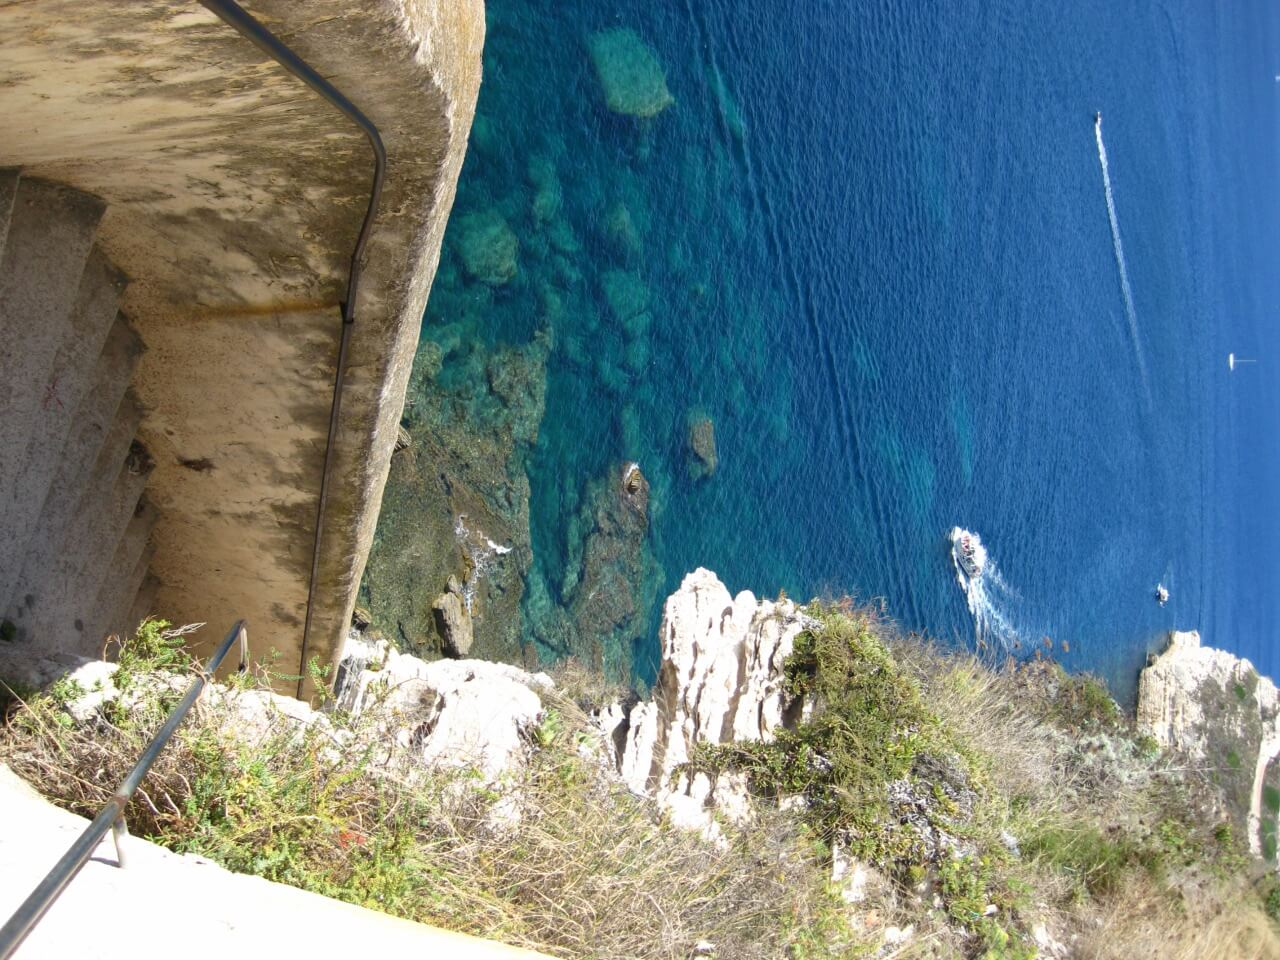
\includegraphics [width=0.3\textwidth]{../Bilder/Korsika/39.jpg}}\quad
   \subfloat{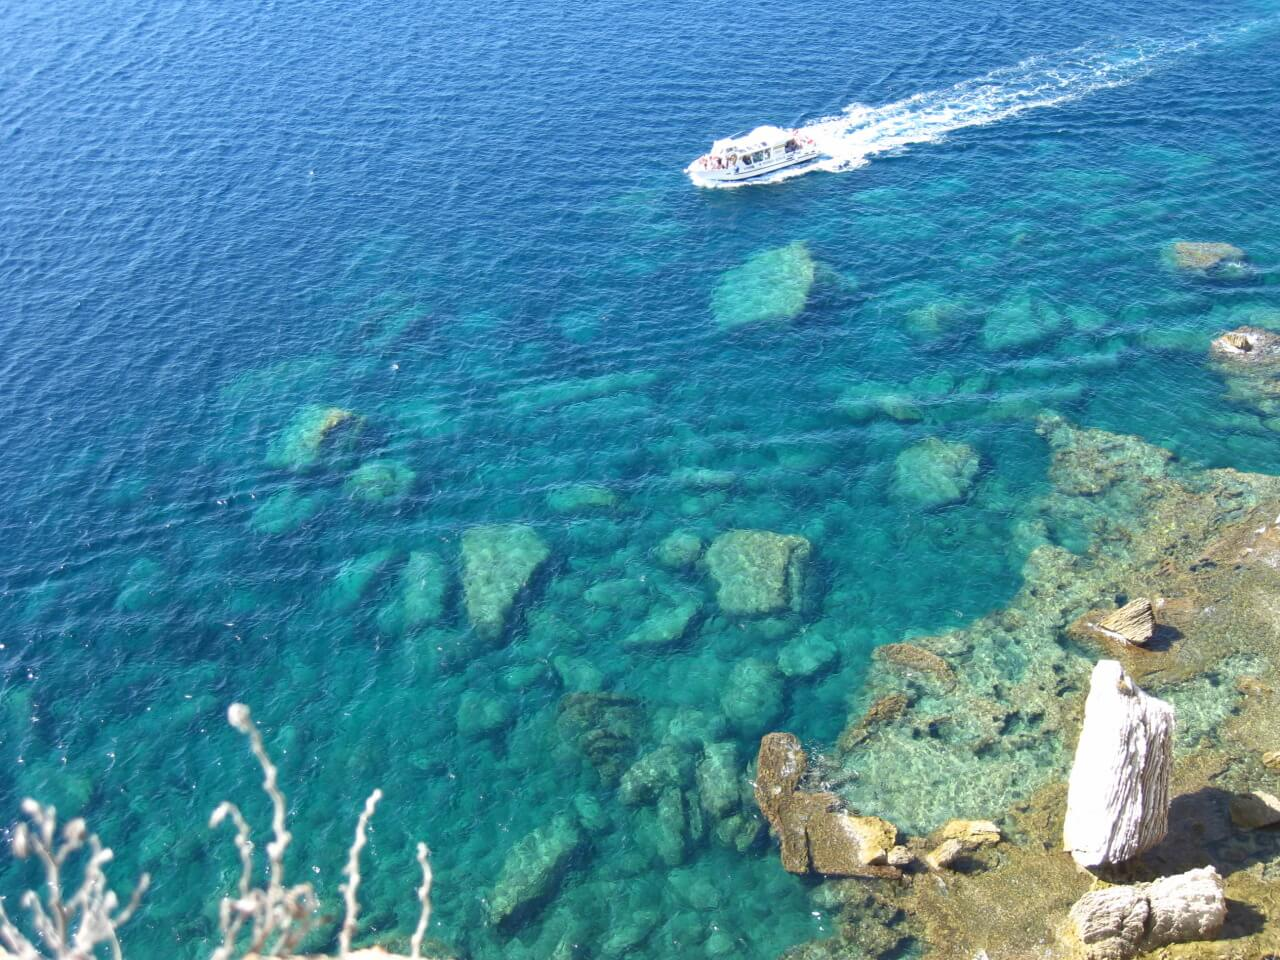
\includegraphics [width=0.3\textwidth]{../Bilder/Korsika/40.jpg}}\quad
   \subfloat{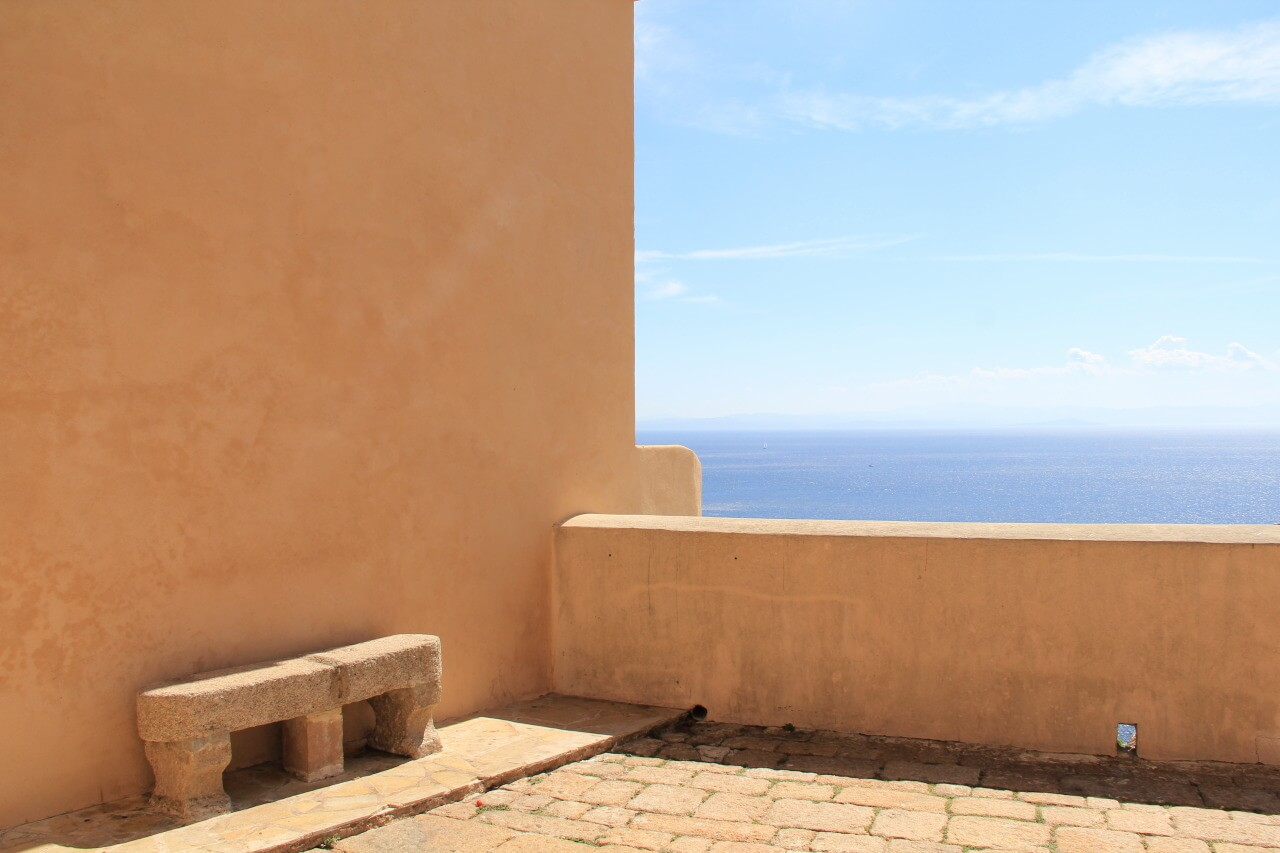
\includegraphics [width=0.3\textwidth]{../Bilder/Korsika/42.jpg}}\quad
   \caption[Idr�ck us Bonifacio]{Idr�ck us Bonifacio}
\end{figure}
Scho vor de 8tne semer h�t ufgstande, wells ade Rezeption gester vo de sehr fr�ndliche Dame gheisse het, wer nachem 8ti zum Beck gat (ein Ma chond jede Morge met sine Br�tli verbi), de chond norno Baguette �ber. So simer fasch Ponkt 8ti zum Becker unter de B�um und hend sogar na Croissant und Schoggi-Br�tli ergatteret. Hmm...fein sends gsi:) Nachem zMorge semer an Strand gh�cklet und send e das glasklare Wasser go schw�mme...esch wondersch�n und erfr�schend gsi. Zrugg ufem T�echli be ich scho gli ipfused und so eschs mer leider de ganz Tag gange...ich be entweder m�ed gsi, be en Trance gsi oder ha sosch chli umetr�umt...en richtigi Schlafm�tze be ich gsi. Aber mer hend trotzdem na es rechts Programm gmacht. Zersch semer es Zentrum vo Propriano go en Bankomat sueche. sSt�dtli esch recht touristisch, aber zemli herzig met de alte Granit-H�ser, de velle L�deli und G�ssli und em chline Hafe. De Bankomat esch zemli versteckt gsi, aber mer hend en schlussendlich doch na gfonde. Mer send de richtig Hafe glofe und hend em feine Duft vo de B�ckereie ned ch�ne widerstah. En Pizza, feini Zuckerb�lleli und e Glace hets ge:) Nach dem Snack simer zrugg zum Jack und witer nach Sartene, skorsiste St�dtli vo Korsika. D�t acho, hemer scho zemli schnell gmerkt, dass es wedermal sehr touristisch esch und mer fasch ke Parkplatz meh findet. Mer hend de doch na eine gfonde und send durs D�rfli gwagglet. Es het sch�ni, uralti und sehr engli G�ssli, aber esch fast zu touristisch, chli wie em Europapark. Nachere Fotisession semer de au scho witer uf Bonifacio, de s�dlichst Ponkt vo Korsika! Zersch hemer na enere Bucht welle go schnorchle oder surfe, aber mer hend nor sone komischi versnobbti, chli langwilligi Bucht gfonde, wo mer ned w�rkli het ch�ne go b�dele. So semer witerzottlet und hend scho gli das wondersch�ne uf Chridefelse baute Bonifacio erblickt. Da mer zersch uf euse Camping hend welle, send mer ade Stadt verbigfahre und send em Pfil Camping dIles gfolget....es esch ewigs gange bes mer denn endli bem Camping acho send. Em Reisef�hrer esch gstande mer cha met em Velo, evt. au zFuess ed Stadt laufe, aber da ch�mer also grad vergesse, es send �pe 8km uf Bonifacio, aber ufe und abe und vor allem ufe. Daher semer de grad do em Camping blebe und send met de Velo an relativ n�che Strand gradlet und send d�t na es St�ndli umeglege. Eigenli h�t die Bucht es Surferparadis s�lle si, aber vo Wind und Welle hemer ned so vell gmerkt. Nachem fulenze und s�nnele semer weder zu eusem Camping zrugd�set, go p�stele und hend zNacht kochet und zwar Ris met Chilli SENZA Carne. Da mer ned grad es mega Men� kochet hend, hemer denkt m�emer dev�r umso meh bem trinke investiere;) de t�rst Wi bes jetzt (14 Euro) hemer kauft, was dVerk�uferi em Lade fasch gschockt het..sie het gmeint: "Cest le plus cher...tu as vu.??"ouioui:) Leider esch er gar ned so fein gsi und ich ha weg mim Chopfweh gar ke Lust meh gha uf Wi. Dev�r ha ich vo mim Schatz e heissi Schoggi becho:) hmm esch super gsi! De Steff het nachli glese und ich be wie en Stei es Bettli plumpst und sofort ipfuused.

\subsection{11.09.2011 Sonntag}
\begin{wrapfigure}{R}{0.45\textwidth} 
  \begin{centering}
    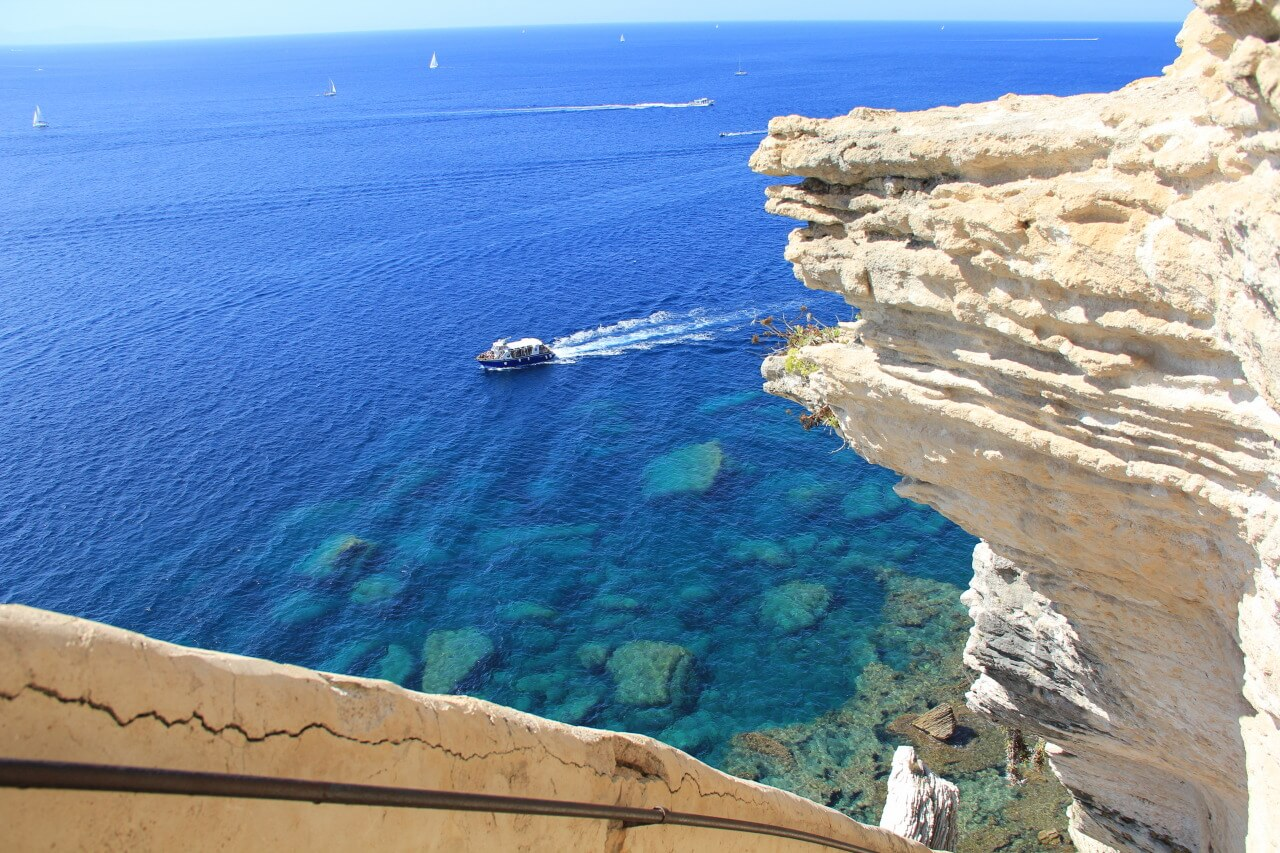
\includegraphics[width=0.4\textwidth, height=5cm, keepaspectratio]{../Bilder/Korsika/38.jpg}
    \caption{Bonifacio}
  \end{centering}
\end{wrapfigure} 
H�t hets feini Croissant und Schoggibr�tli zum zMorge ge. Gm�etlich hemers gno und send de um di 11i uf Bonifacio..wow die Stadt esch echt de Hammer! Zersch semer am Hafe umegschlenderet, wo de Steff ganz vell riiiiesigi Jachte bestunt het und fasch chli ifers�chtig worde esch. Neb de Schiff hets ganz vell Restaurants, Kaffis und Bars gha. De simer ufegwanderet ed Oberstadt vo Bonifacio,wos eus gfalle het und mer paar St�ndli verbrocht hend. Bonifacio esch uf steile, zum Teil �berh�ngende Chridefelse baut und daher sehr imposant. De Ufstieg ed Altstadt esch dementsprechend au zemli astrengend gsi, abere het sich uf all F�ll glohnt. Die ganz Oberstadt esch nemli voll vo herzigi G�ssli met vellne Restaurants, Souvenir-L�de und Kaffis. Zw�sched inne hesch na en super Ussecht vode Chridefelse abe uf das traumhafte-glasklare Meer. Zum Zmettag hemer e chli en grossi Thunpizza und feini Crevette gha:) Denn semer na uf de H�gel visavis vode Altstadt gloffe und hend vo d�t en geniali Ussecht uf dOberstadt unds Meer gha. Bem Abstieg ha ich fasch na es Herzchriesi becho, well churz vor mer en riiesige Schlange verbigschl�nglet esch...u���! De Steff het zersch n�t metbecho, well er sine Flugis nacheglueget het, ersch wo ich umegschroue und umegumpet be, het er sich gfragt, was e mich gfahre esch. Nach dem velle Umelaufe semer recht kaputti gsi und hend eus chli m�esse ufeme B�nkli erhole. Da aber ersch 4i gsi esch und mer na hend welle zNachtesse en Bonifacio, hemer na paar St�ndli vor eus gha. Darum hemer denkt: Mached mer doch na e chlini Bootstour:) Am 5i semer de met eme B�tli usem Hafe gfahre und send grad e di erscht Grotte inegfahre..wow..t�rkis-glasklars Wasser, Tropfstei und Chridefelse..het supersch� usgseh! De semer witer zode Lavazzi-Insle zo de Riche und Sch�ne und de weder zrug uf Bonifacio. Em sch�ne Obigsliecht het dAltstadt grandios usgseh und mer hend wedermal einigi F�teli gmacht. Mer het w�rkli sG�hl, die H�ser gheiet n�chstens grad es Wasser. Die steil Aragon-Treppe hemer vo witem au bestunt. Die semer am Mittag abeglofe und send fasziniert gsi vo de sch�ne Felse und dem traumhafte Wasser. Nor vom Ufstieg semer de n�m so begeisteret gsi;) dB�tlitour esch sehr erfr�schend gsi. Trotzdem semer zrug em Hafe enes Kaffi go en Ap�ro neh...uiuiui...mer eschs nacher zemli guet gange;) Min Moon-Drink het echli vell Prosecco denne gha, so dass ich grad es Glas umgschmisse ha. Leider esch em Steff sin Rucksack dusched worde. De semer enes Resti gschwankt;) und hend sehr fein zNachtgesse. Damol hets Seet�fel met Pfeffersauce und St.Pierre met N�ssli und Ris und Gm�es geh. Um di 10ni semer de zrug zo eusem Jack und uf de Campingplatz d�set. Esch en supersch�ne Tag gsi:)

\subsection{12.09.2011 Montag}
\begin{figure}[b]
   \centering
      %\subfloat[CAPTION]{BILDERCODE}\qquad
   \subfloat{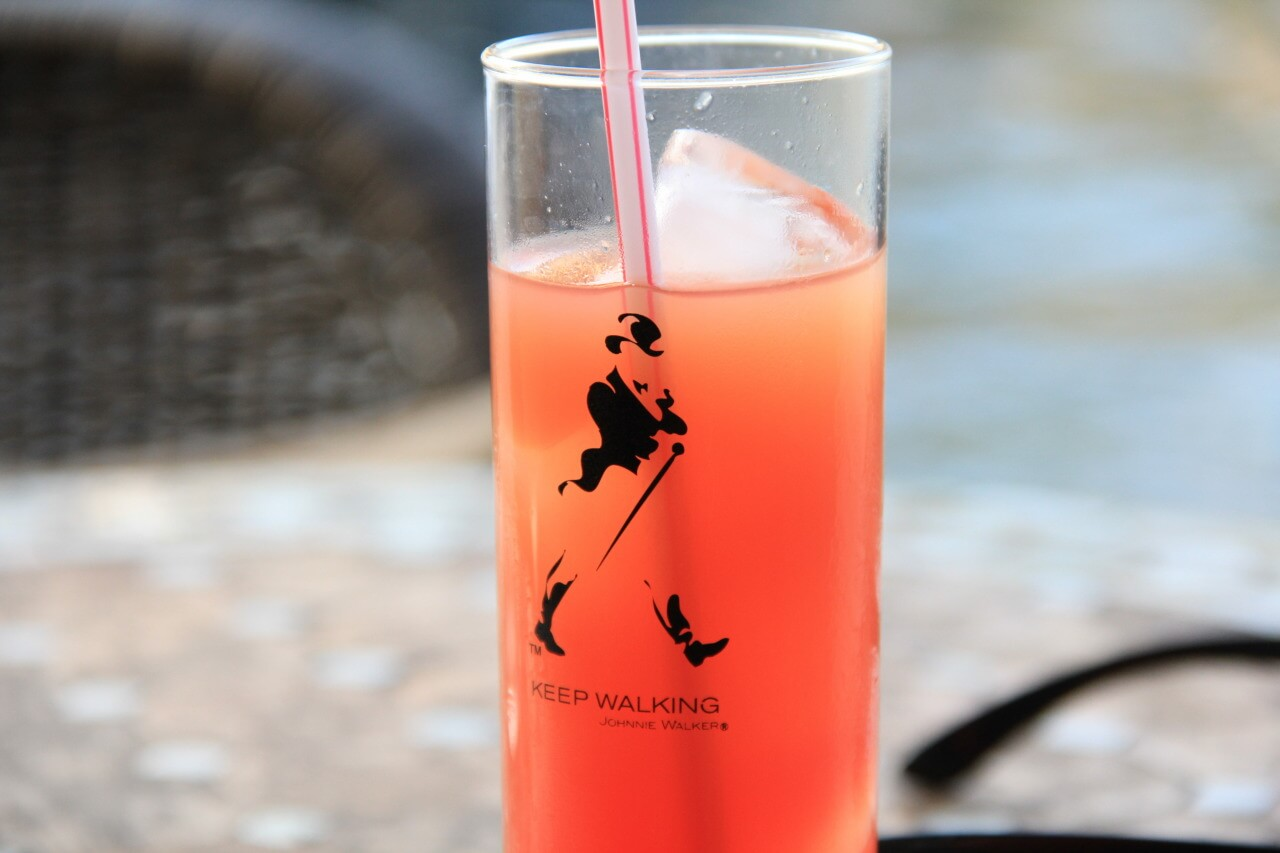
\includegraphics [width=0.3\textwidth]{../Bilder/Korsika/49.jpg}}\quad
   \subfloat{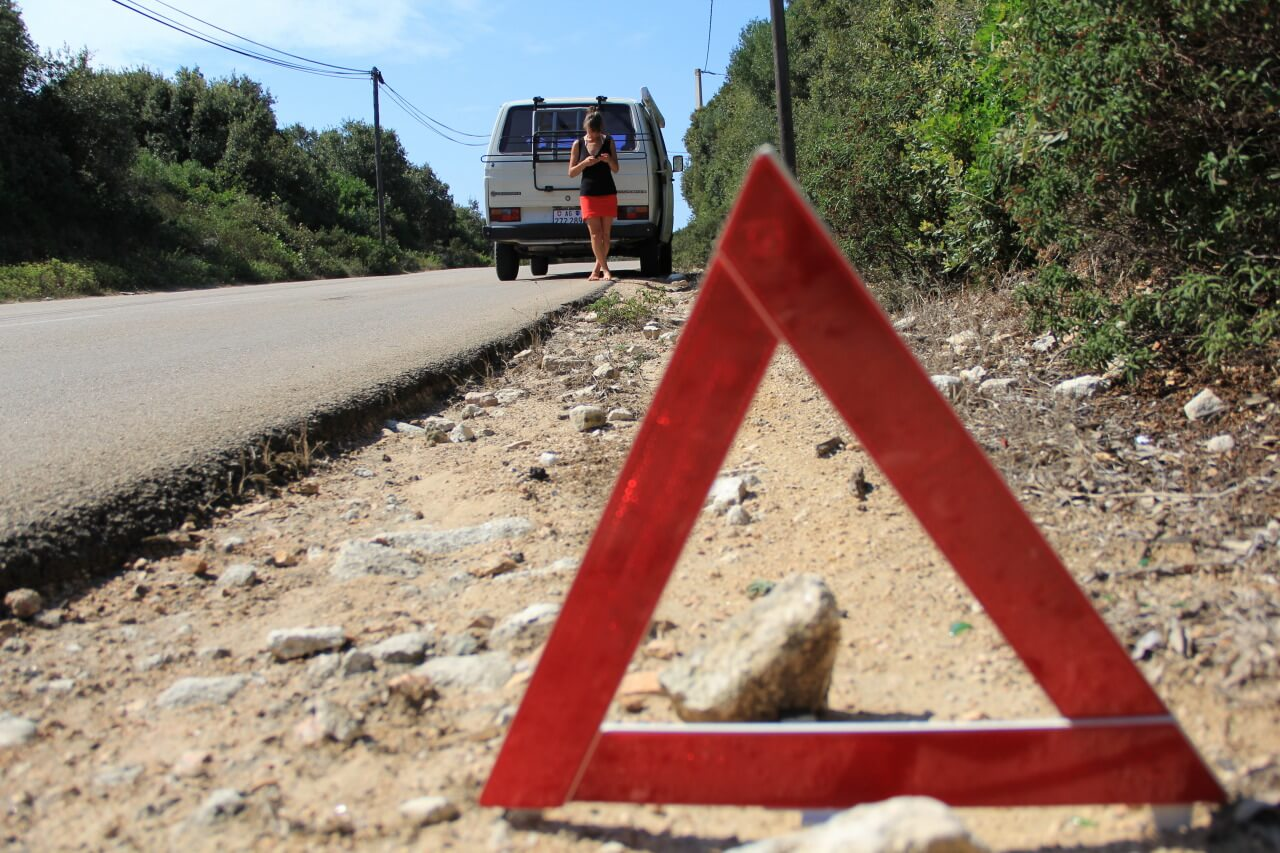
\includegraphics [width=0.3\textwidth]{../Bilder/Korsika/50.jpg}}\quad
   \subfloat{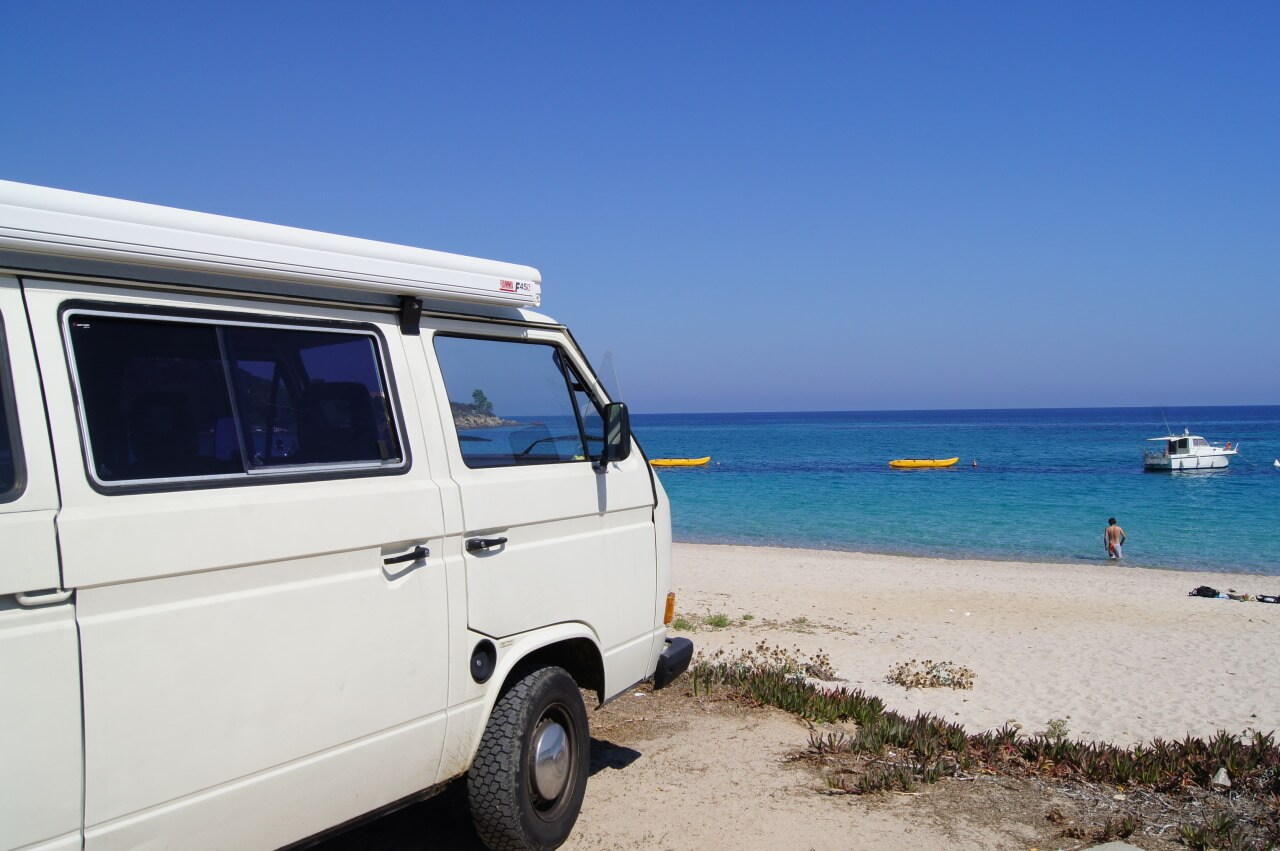
\includegraphics [width=0.3\textwidth]{../Bilder/Korsika/51.jpg}}\quad
   \caption[Pannentag]{Pannentag}
\end{figure}

Der Pechstag...fit und munter simer ufgstande,hend zm�rgelet und hend eus uf de Weg nach Bonifacio gmacht.
D�t hemer ghofft en schrubeziehr zfinde, um dKeilrieme vom jack ch�ne zflicke,da de so komischi Gr�sch vo sich get und internet, um mis Sprachmodul zBueche.
Beides hemer eigentli gschafft und trotzdem esch �pis ed Hose.
Ich ha am Hafe eme Internetkaffi ch�ne bueche und de Steff het zueff�llig en chline Werkz�glade gfonde.
Gl�cklich simer zrugg zu eusem Camping gfahre.
Ufem weg dethi hemer dKeilrieme na azoge und denkt;jetzt cha n�t meh schief ga;-) Leider hemer da falsch gedacht...
ufem Weg zo de supersch�ne Rondinarabucht,wo mer hend welle go b�dele, het euse Jack schlapp gmacht:-\ dKeilrieme send grisse und de Motor het gsprudlet..ohoh..
Das het ned guet usgseh.
Nachdem de Steff es paar mal probiert het die Rieme weder anezmache unds ned klappt het, hemer eusi Hoffnige ufgeh und hend em TCS agl�te.
Die hend gmeint: e einere Stond werdet er abgschleppet.
So hemer e eusem B�sli gwartet und gwartet.
De esch endli sAbschleppauto cho...
de Fahrer het ke Muks gseit,het de Jack ufglade und eus gfr�gt,�b mer wend metcho...
a klar hemer da welle,was h�ttet mer sosch s�lle mache? Wo mer gfr�get hend wos hi gat, het er gseit, nach porto veccio,d�t s�g di n�chst vw-garage.
Da simer grad chli verschrocke, da mer denkt hend mer g�nd enen Werkstatt en Bonifacio.
Aber Porto Veccio esch nor e halb Stond entfernt gsi.
Be de VW Garage acho, esch de Jack abglade worde und de Schleppwaage esch schoweder abd�set.
Mer send de inne go frage, wie lang dReperatur werd ga, da hend si nome gmeint; h�t werd er eh n�m aglueget, ersch morn morge und de meldet sie sich...
vorhe cha mer n�t s�ge.
Na super...so simer de H�gel ufe es Zentrum vo Porto Veccio zottlet und hend eus uf dSuechi vome Hotel gmacht.
Das esch gar ned so eifach gsi...
eis nachem andere h�mer abklapperet,aber leider n�t gfonde, alles esch complet gsi! Scho fasch hemer dHoffnig ufgeh und eus met em Gedanke vertraut gmacht am Strand zschlofe, als em letzte Hotel womer gfr�get hend, zwar au alles voll gsi esch, aber na es Abstellch�mmerli frei gsi esch.
Nat�rli hemer zuegseit und es esch gar ned so es chlises Zemmerli gsi.
Es het e Duschi, es WC(openair) und sogar en Fernseh gha.
Mer hend eus chic gmacht f�rs zNachtesse und send ed Altstadt vo Porto-Veccio.
St�dtli esch wondersch�n gsi met de velle chline,herzige und gm�etliche Restaurants,Kaffis und L�deli, wo sich ede enge G�ssli versteckt hend.
Znachtgesse hemer emene guete Resti ufere Terrasse, wo mer direkt uf de Hafe abe gseh het...wow...esch genial gsi!sEsse esch au himmlisch gsi! Mer hend grad es ganzes Men� gno: Rohschinke met Melone, Wildschweinlasagne, Penne met Lachs, Glace und �pfelchueche.
De Vollmond esch de na ufgange und es esch en wondersch�ne Obe gsi:-) Es het sich doch na zumene Gl�ckstag gwendet;-)

\subsection{13.09.2011 Dienstag}

\begin{wrapfigure}{R}{0.45\textwidth} 
  \begin{centering}
    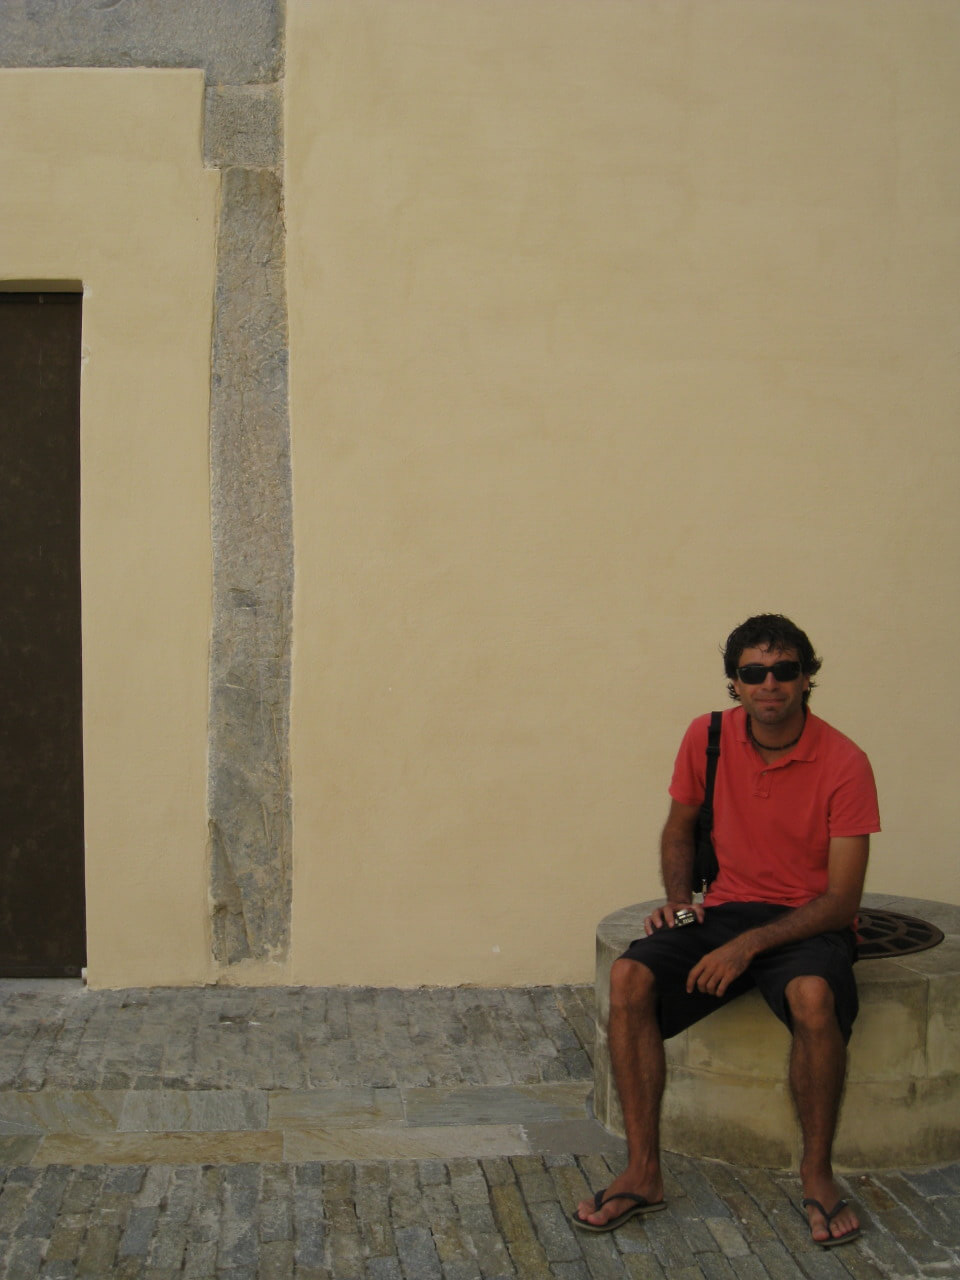
\includegraphics[width=0.4\textwidth, height=5cm, keepaspectratio]{../Bilder/Korsika/52.jpg}
    \caption{Ohni Bus unterwegs...}
  \end{centering}
\end{wrapfigure} 

Nachere vell zwarme Nacht und dementsprechend ned ganz so fit, simer uf de Garteterrasse vom Hotel fein go zm�rgele.
Gst�rkt simer ed VW Garage gloffe und hend ghofft, sie ch�nd eus scho meh Uskunft geh.
Aber wie erwartet esch na nix gange sie hend gseit, sie luegets am Namittag a...
uhh da ha ich schochli afo brodle und dampfe...
es het so t�nt,wie sie en am donnstig mal alueget und de mal lueget was zmache esch und keilrieme wahrschinli na m�end bstelle..grr..
mer hend de gseit, dass mer am Donnstig abreiset und so schnell wie m�glich s�tt gmacht werde.
Serschte wo mer jetzt hend welle, esch es Mietauto gsi, well mer emmerna eusi St�ehl, Tisch und Velos em Camping be Bonifaciogha hend und mer m�ed gsi send vom velle umelaufe.
So hemer em TCS agl�te, welli eus versicheret hen, dass sie eus es Mietauto organisieretund wo eus grad be de Garage abholt.
WOW..das esch na Service hemer denkt und send erliechteret noimet abgh�cklet und hend gwartet.
Nach �ber e Stond hemer eus langsam gfr�get, wo euses Auto esch, nach 2 Stond hemer namal agl�te.
De hets gheisse: ah ja ich ha ene grad welle al�te, sAuto staht parat bem Europcar! Jaja grad welle al�te, mer wartet 2 Stondund niemert informiert eus, echt en Frechheit! E dere Zyt h�ttet mer scho laang selber es Auto gmietet! Mer hend vermuetet, dass de Europcar bem Flughae esch und mer es Taxi m�end sueche. Da mer aber kes Taxi gfonde hend, semer enes Resti und hend d�t nach de Taxi-Telefonnummere gfr�get.
Zum Gl�ck het sie eus de gseit, dass Europcar grad um de Ecke esch, zum Gl�ck! Aber da de ersch weder am 2 ufgmacht het, hemer nachli Zit m�esse vertribe.
So simer nachli go shoppe:-) Mer send sogar erfolgrich gsi und es het neui Badhose, Hemdli und Flipflops geh.
Sauto hemer am 2 ch�ne abhole und so simer de au endli eusi verlorene Campingsache go hole.
Da mer eigentli scho laang hend welle go b�dele, simer de na gschnell an Strand gh�cklet.
Denn het de Steff e suuuper Nachricht becho: Euse Jack esch gflickt und abholbereit,jupiii! Schnell simer zode Garage d�set, hend de Jack gholt, sMietauto weder zruggeh und de sch�ni Camping Rondinara gfahre.
D�t hemer fein zNachtgesse(Tortellini) und send de gli go pfuse, da mer zemli m�ed gsi send.
Aber au sehr gl�cklich, well mer euse Jack weder gha hend:-)

\subsection{14.09.2011 Mittwoch}
Strandtag, jupiii :) H�t semer de gaaaaaaaanz Tag am wondersch�ne Rondinarastrand glege, hend gs�nnelet und b�delet.
sMeer esch glasklar und so sch�n t�rkis gsi, wie uf de Maledive.
Zum Bade esch es eifach traumhaft gsi.
Nebem ful umelege, hemer nachli Speedmington gspelt, was aber dank em Wind gar ned so eifach gsi esch.
Denn semer na go schnorchle.
De Steff esch extra am Mittag be gr�sster Hitz de steil Weg zum Camping ufegloffe und het eusi Schnorchelsache...
leider hets sich ned glohnt, well mer ussert paar chline Feschli und es paar Felse ned vell gseh het.
Dev�r hets sich glohnt, dass mer es Bodyboard kauft und mitgschleikt hend.
Wells ade Ostk�ste sooo hochi Welle gha het, hemer eus eher gf�hlt wie gstrandeti Wale als wie Surfer;-)
Zmettaggesse hemer em sch�ne Strandrestaurant.
Um di 6i semer zrug zo eusem Camping und hend euses zNacht vorbereitet, Ratatouille met Ris und feinem Ros�.
Nachem Esse hemer na �ber Gott und die Welt plauderet und send de ab es Bettli..
met emene chli warme, sonneuftankte Chopf.
Ou �pis hani na vergesse...
mer h�ttet eigentli super gschlafe, wenn euse liebi Nachbar, wo zersch e Liechtshow abzoge het, ned so lut gschnarchlet h�tt, dass de ganz Camping bebt h�tt und am Morge rings um en ume alli gfl�chtet send.

\subsection{15.09.2011 Donnerstag}
H�t heisst ab nach Bastia! Fr�e semer ufgstande und hend eus uf de Weg gmacht in Norde vo Korsika.
Zersch esch de Steff die voll krassi und kurverichigi Stross vom Camping zruggfahre und witer bis zume supersch�ne Sandstrand n�rdlich vo Porto Vecchio.
D�t semer zum letschte Mal namal e das wondersch�ne Meer gumpet und hends eifach gnosse.
Denn han ich denkt, jetzt cha ich witerfahre, send ja sch�ni, gradi und breiti Strasse...
esch au alles guet gange, bes mich es fetts Hummeli es F�dli gstoche het! Auuuua! Ich be ufgspronge, has St�rrad losglo, has Hummeli wegworfe und da hets mi grad namal en Finger gstoche! De Steff hets St�rrad m�esse �berneh, denn ha ich mich weder chli beruhigt und be uf dSite gfahre, usgstege und umegsprunge...haha..
de Steff het weder m�esse witerfahre und ich hami nebeddra versuechts erhole..
was gar ned so eifach gsi esch, wenn mer ned ufs F�dli cha hocke:-P
En Bastia acho, semer namal chli an Strand gh�cklet und send de es Zentrum an Hafe go zNachtesse.
Nachem Esse hemer na en Camping m�esse sueche und hend eus f�r de stadtn�chsti Platz entschede, wo ned w�rkli sch�n gsi esch, aber dev�r direkt am Meer.

\begin{figure}[H]
    \centering
    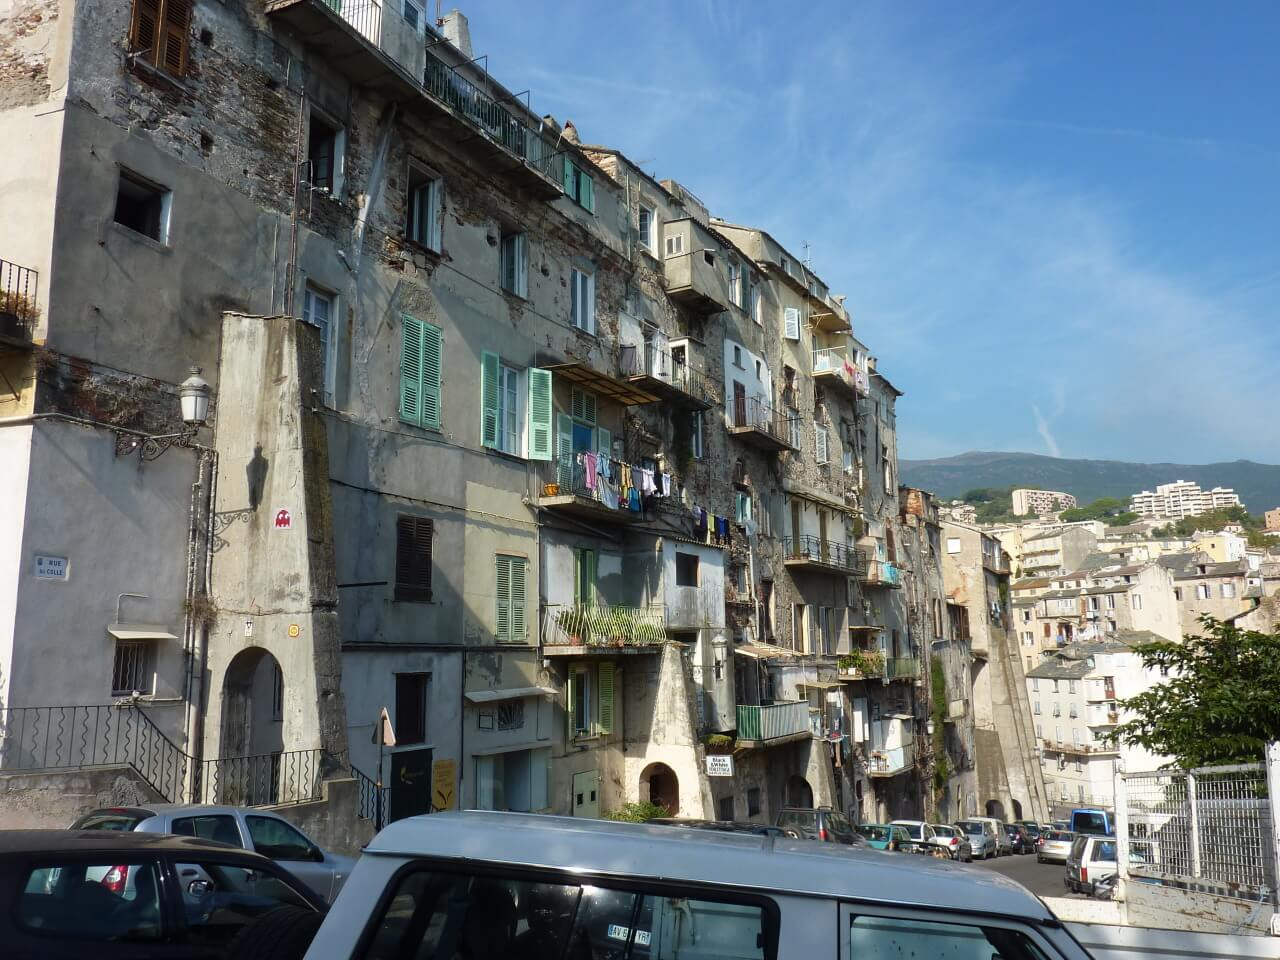
\includegraphics[width=\textwidth]{../Bilder/Korsika/53.jpg}
    \caption{Bastia}
    \label{img:Korsika3}
\end{figure}

\subsection{16.09.2011 Freitag}
H�t morge hemer die sch�ne sanit�re Anlage vo eusem super Campingplatz kenneglernt...
wu��� und de hends na neb eus sAbwasser abgloh.
Mer send de schnell uf Bastia innegfahre und hend ede sch�ne Altstadt zm�rgelet met wondersch�ne Ussecht uf de Hafe.
Mer send nachli ede Stadt umegschlenderet und hend de dF�hri ufgsuecht.
Die esch lang ned ume gsi, het sich de aber doch na blicke lo und de esch alles schnell gange.
Schlossendlich semer fascht rechtzitig abgfahre.
Mer hend euse Jack parkiert, send ufs Deck gst�rmt und hend na en Platz ergatteret zum s�nnele:) Die n�chste 5 Stond hemer met lese, s�nnele, Bricht schribe und esse verbracht;) En Genua acho, semer grad witergfahre durs Aostatal, wo mer fasch uf jedem H�gel sch�nbel�chteti Ruine gseh hend und dur de Gross Sankt Bernard, was 35 Franke kostet het.
Uf Sion het sichs de doch na lang zoge.
Ersch am halbi 2 semer en Sion acho und hend nebere Fabrik es �bernachtigspl�tzli gfonde.
M�ed vode lange Reis, aber gspannt uf dFlugshow morn, semer grad es Bett gheit und ipfused.

\begin{figure}[H]
    \centering
    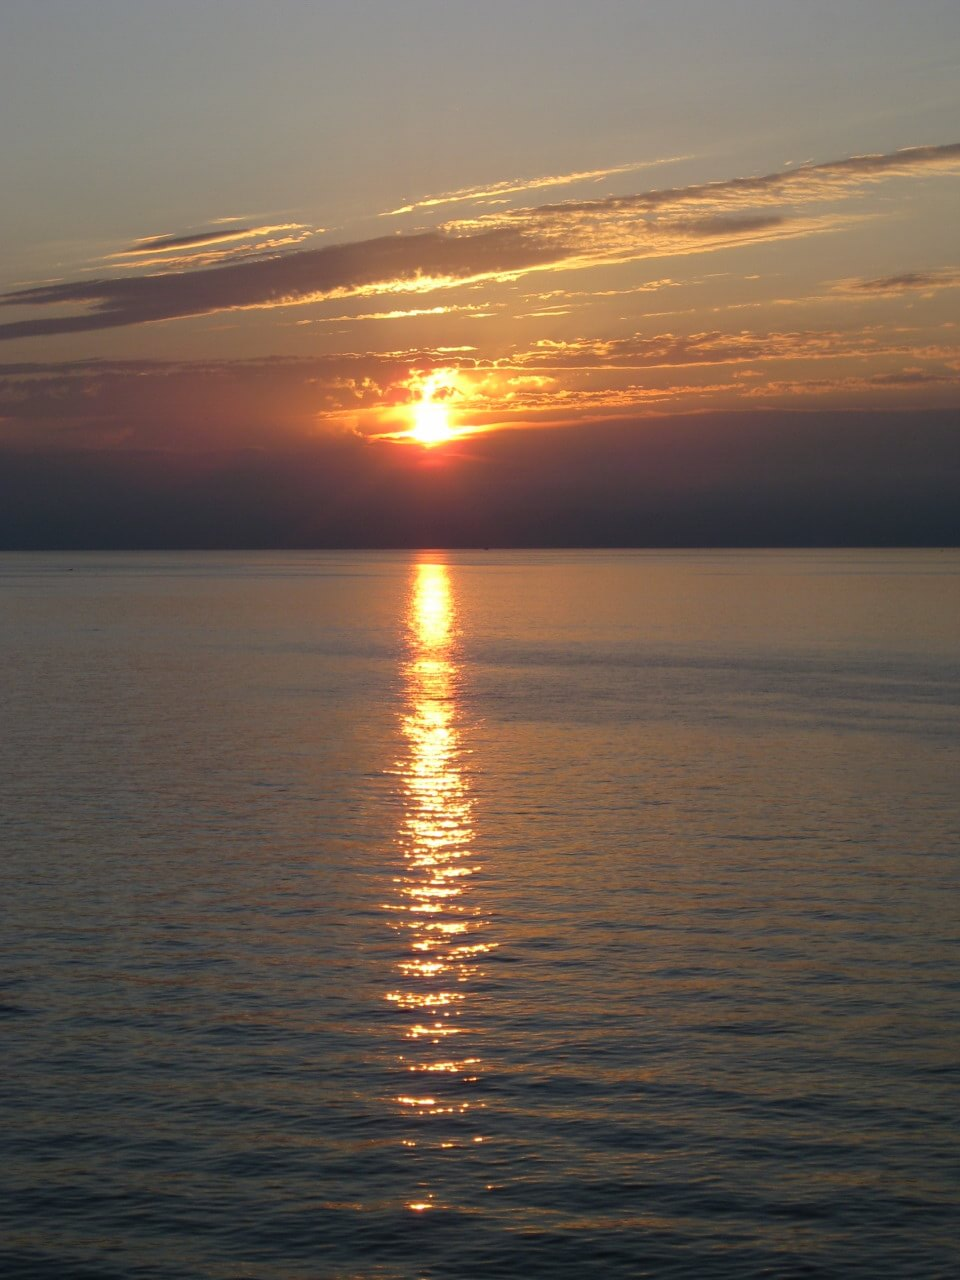
\includegraphics[width=\textwidth]{../Bilder/Korsika/54.jpg}
    \caption{Herrlichi Ferien gsi}
    \label{img:Korsika4}
\end{figure}

\newpage
\section{Aegerisee 2012}
%    JJJ    AA     CCCCCC KKK   K TTTTTT HH  HH EEEEEE BBBBBB UU  UU SSSSSS    CCCCCC OOOOOO MM  MM
%    JJJ   AAAA    CCCCCC KKK  K  TTTTTT HH  HH EEEEEE BB   B UU  UU SSS       CCCCCC OOOOOO MM  MM
%    JJJ  AA  AA   CC     KKK K     TT   HHHHHH EEE    BB   B UU  UU SSS       CC     OO  OO MMMMMM
%    JJJ AA    AA  CC     KKKK      TT   HHHHHH EEEEEE BBBBBB UU  UU  SSSSS    CC     OO  OO M MM M
%    JJJ AAAAAAAA  CC     KKK K     TT   HH  HH EEE    BB   B UU  UU    SSS    CC     OO  OO M MM M
% JJJJJJ AA    AA  CCCCCC KKK  K    TT   HH  HH EEEEEE BB   B UUUUUU    SSS .. CCCCCC OOOOOO M MM M
% JJJJJJ AA    AA  CCCCCC KKK   K   TT   HH  HH EEEEEE BBBBBB UUUUUU SSSSSS .. CCCCCC OOOOOO M MM M
% 
% Texte Geschrieben von Stefan Bopp und Chantal Frunz
% Mehr Informationen sind auf jackthebus.com zu finden
%

\subsection{Freitag 06.04.2012}
Aus der geplanten fr�hen Abfahrt Richtung Zug wurde nichts.
Das Wetter zeigte sich leider eher von der bescheidenen Seite und so beschlossen wir das Ganze gem�tlich anzugehen.
Den Einkauf habe ich schon am Vortage erledigt und auch Jack stand nach etlichen kleinen Ungereimtheiten wieder frisch da.
Die erste �berraschung gab es schon vor der Abfahrt.
Mein Fahrrad entschied sich die Luft des Pneus wieder der Umwelt zuzuf�hren.
Gl�cklicherweise steht im Keller noch ein zweites und der Umweg um es aufzuladen h�lt sich in Grenzen.
Die Fahrt verlief Ereignislos und schon bald konnten wir unsere Fahrr�der satteln und eine kleine Tour um den See zu starten.
Es war zwar nicht gerade strahlender Sonnenschein aber trotzdem hielt sich das Wetter.
Der kurzfristige Wechsel des fahrbaren Drahtgestells f�hrte dann auf dem Waldweg zu Herausforderungen, welche mit einem "`anst�ndigen"' Velo so nicht zu meistern gewesen w�ren.
Nach einer kurzen St�rkung in Unter�geri schlossen wir die erfolgreiche Umrundung des Sees ab und begaben uns kurz nach 14 Uhr zum Campingplatz, welcher uns f�r die n�chsten zwei Tage beherbergen sollte.

Da der Platz bei den m�ssigen Wettervorhersagen nicht gerade �bervoll war, konnten wir uns einen Stellplatz aussuchen und positionierten uns in unmittelbare N�he des Sees.
Als Nachbarn tauchten schon bald B.A Baracus und ein weiblicher Colonel John Smith mit einem genauen Imitat des bekannten Vans auf.
Unsere kleine mitgebrachte Heizung musste schon jetzt ihre Standfestigkeit unter Beweis stellen, da Chantal sich ohne Schlafsack nicht mehr aus dem aufgebauten Bett hervortraute.
Die zweite B�chse Chili con Carne, welche wir in Bonifacio letzten Sommer k�uflich erworben haben, diente mir als willkommene Mahlzeit nach der kurzen Velotour.
Frisch gest�rkt ging es an den Strand.
Sogar die Enten zog es an Land, die Temperaturen waren eher frostig. 
Nach dem Duschen, welches unerwartet unsere 50erli aufbrauchte, war es an der Zeit etwas zu kochen.
Die Temperaturen waren zwar tief, trotzdem entschieden wir uns vor dem Bus zu essen.
Nach dem obligaten Abwasch (der gerade Chantal immer wieder Spass macht) haben wir uns in den Bus verkrochen und unser Elektro�feli das erste Mal so richtig gefordert.

\begin{figure}[H]
   \centering
      %\subfloat[CAPTION]{BILDERCODE}\qquad
   \subfloat{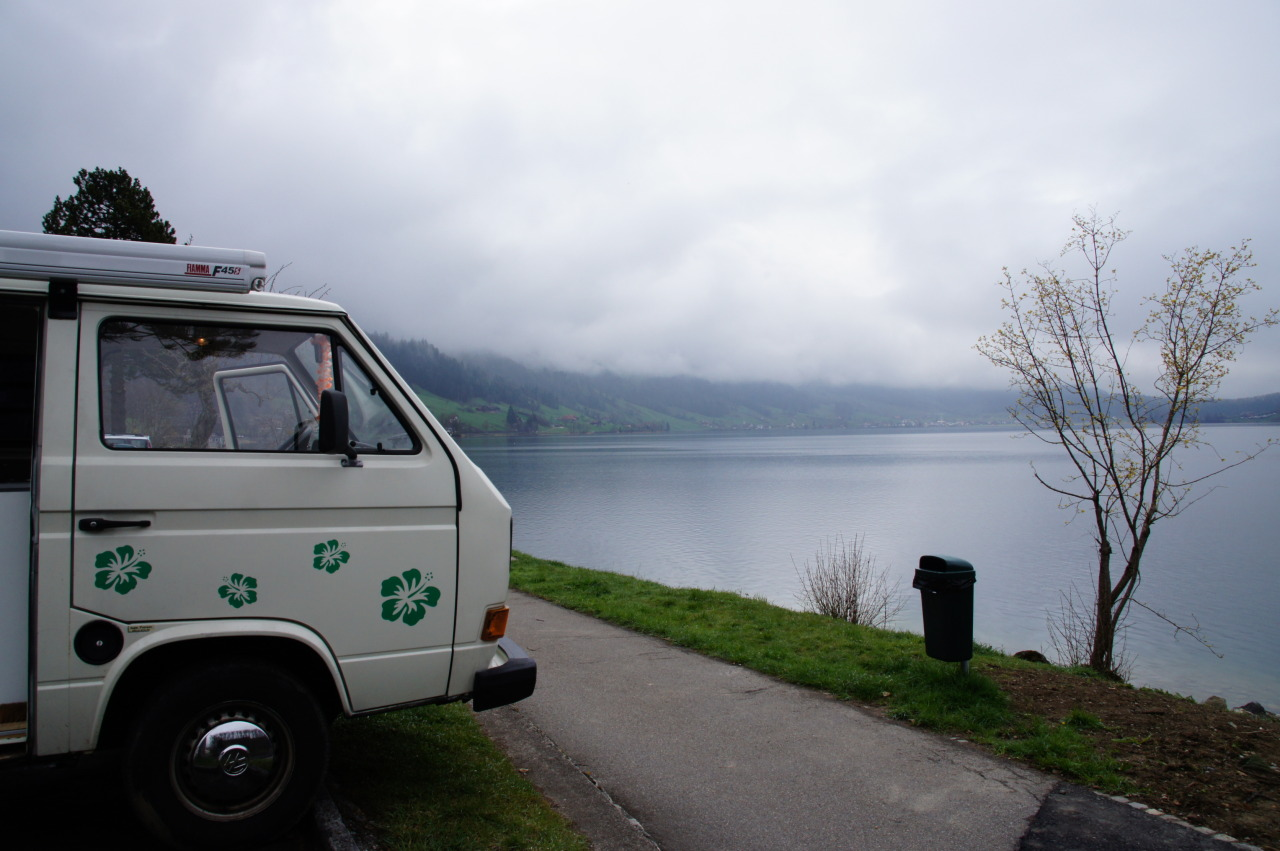
\includegraphics [width=0.3\textwidth]{../Bilder/Aegeri/1.jpg}}\quad
   \subfloat{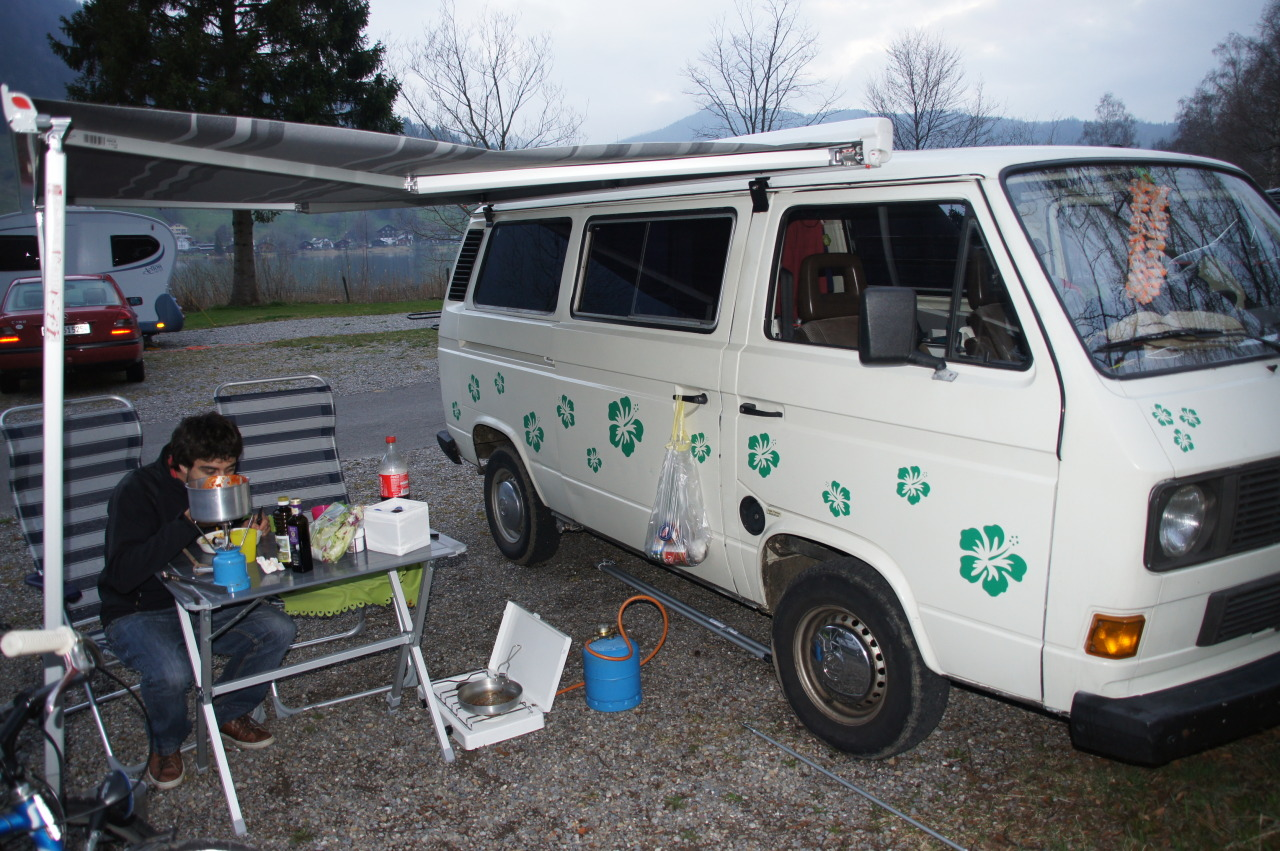
\includegraphics [width=0.3\textwidth]{../Bilder/Aegeri/4.jpg}}\quad
   \subfloat{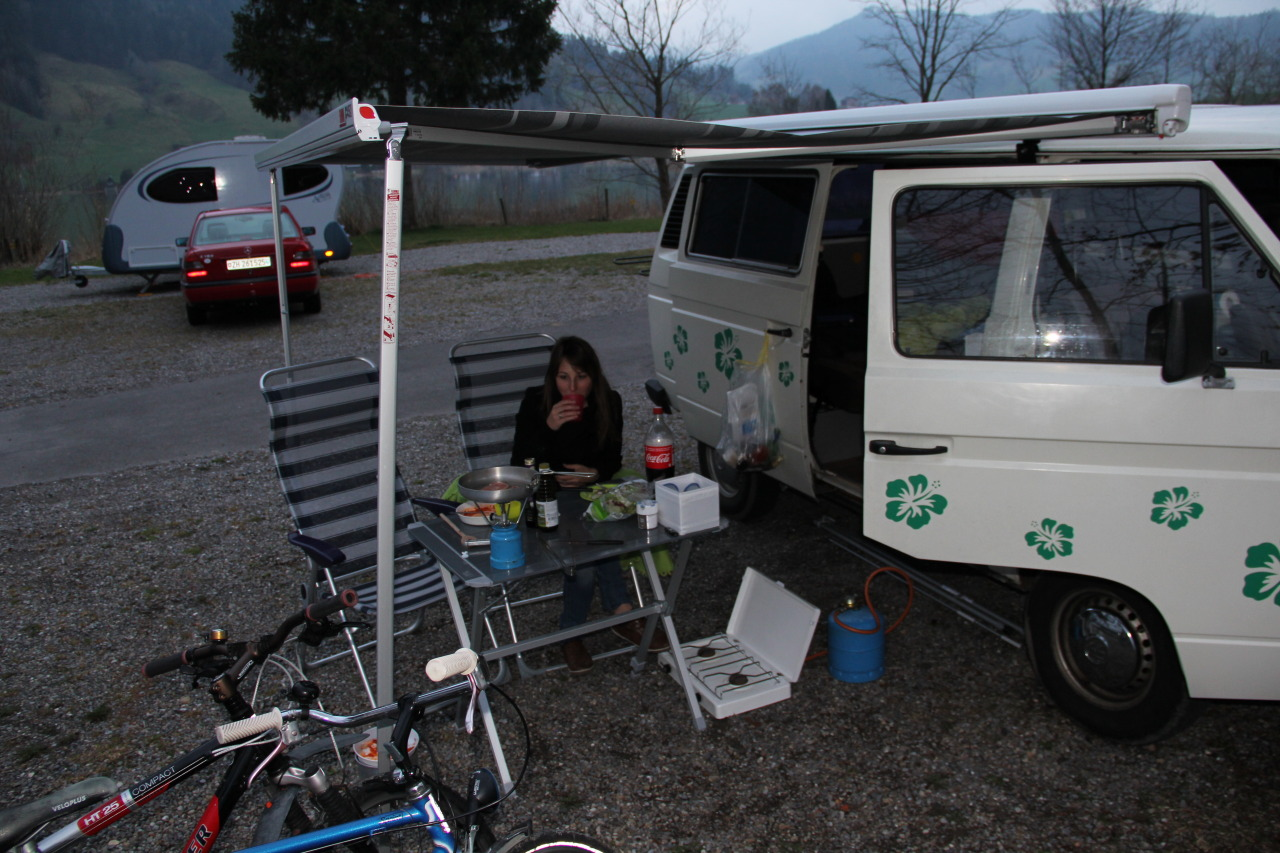
\includegraphics [width=0.3\textwidth]{../Bilder/Aegeri/7.jpg}}\quad
   \caption[Auf dem Campingplatz]{Auf dem Campingplatz}
\end{figure}

\subsection{Samstag 07.04.2012}
Der Samstag zeigte sich vom Wetter her leider noch trister.
Es regnete sehr stark und wir beschlossen noch ein wenig l�nger liegen zu bleiben.
Zuerst wollten wir mit den �V richtig Zug aufbrechen.
Die Wassermassen die vom Himmel fielen, �berzeugten uns jedoch bald den VW-Bus zu nehmen.
Nach einem ausgewogenen Fr�hst�ck im Bus mussten wir uns auf den Weg machen, da wir sonst bei der Ausfahrt die so heilige Mittagsruhe auf dem Campingplatz verletzt h�tten.

\begin{figure}[t]
    \centering
    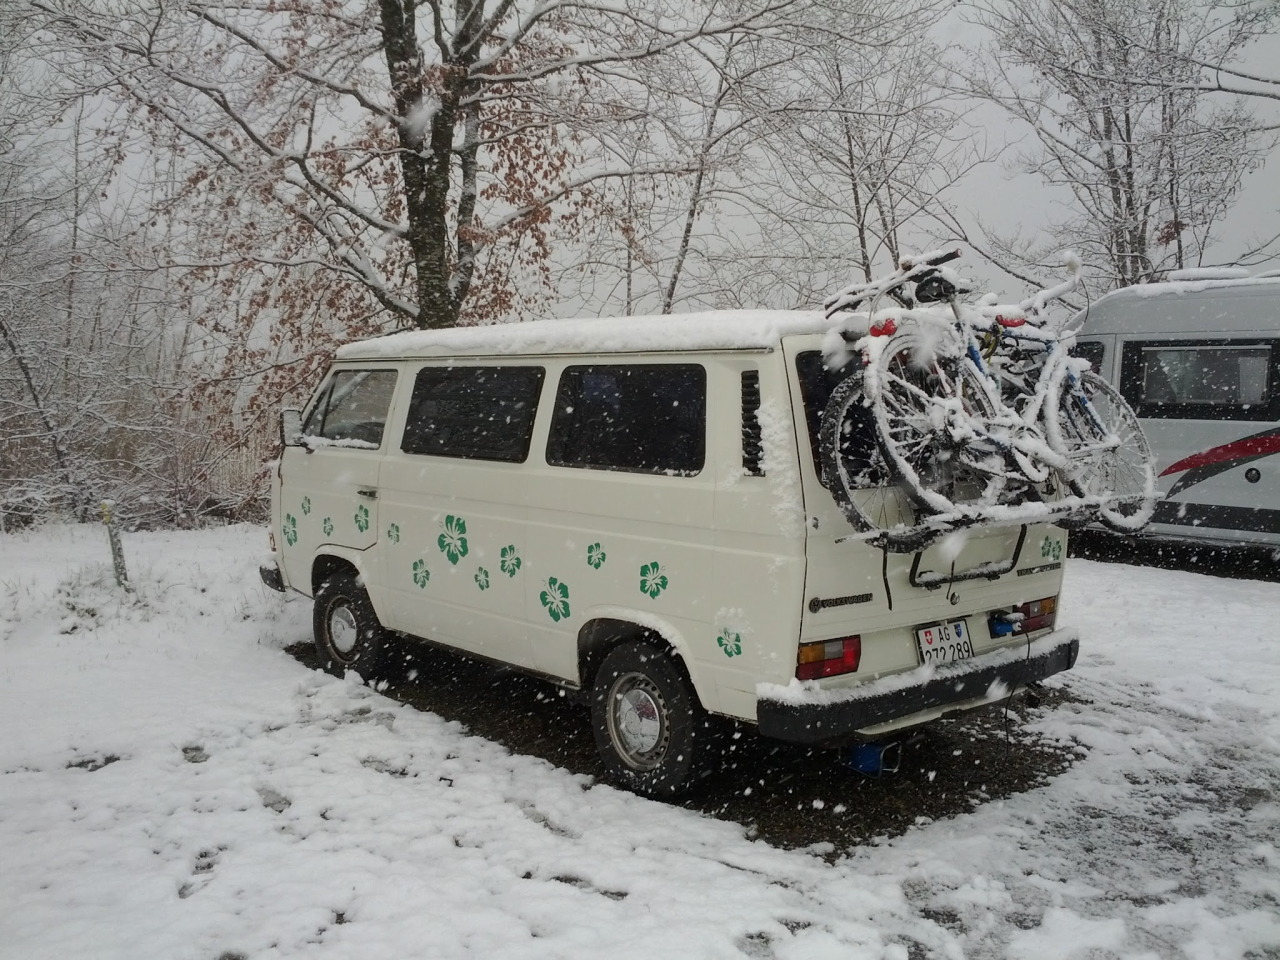
\includegraphics[width=\textwidth]{../Bilder/Aegeri/11.jpg}
    \caption{Vom Winter eingeholt...}
    \label{img:Dolomiten}
\end{figure}

Das Parkhaus war schnell gefunden worden und wir machten uns auf, Zug shoppingtechnisch zu erkunden.
Eher eine Qualit�t, welche Chantal mit sich bringt.
Nach etlichen abgeklapperten Shops und eingelegten Trinkpausen war da ein leichtes Ziehen in der Magengegend zu versp�ren.
Dieses �usserste sich bald etwas heftiger bei Chantal und wuchs schnell einmal zu einem Verlangen nach fester Nahrung an.
Bl�derweise war es Mitten am Nachmittag an einem Ostersamstag.
Die Frage nach warmen Essen am Nachmittag, welche in einer Pizzeria gestellt wurde, ist zwar positiv beantwortet worden.
Die eingeschr�nkte Karte konnte Chantal jedoch nicht �berzeugen und so reservierten wir einen Tisch um 18:00 Uhr.
Fast zwei Stunden mussten wir noch �berstehen und das, nachdem der intensive Pizzageruch meinen Kohldampf wieder geweckt hat.

Nach einem Besuch der Burg und einem kleinen Ap�ro, begaben wir uns ins Restaurant und genossen ein herrliches Nachtessen.
Den restlichen Abend verbrachten wir mit der Suche meines Autoschl�ssels und Witzen was das Wetter noch alles bringen wird.

\subsection{R�ckfahrt}
Sch�n! Kein Getropfe zu h�ren.
Nur das ratternde Ger�usch des �felis.
Es hat aufgeh�rt zu regnen.
Tats�chlich regnete es nicht mehr.
Es hat angefangen zu schneien!! Unsere Markise �chzte schon unter der weissen Pracht.
Tapfer entstieg ich dem warmen Auto und befreite todesmutig den arg gebeutelten Stoff von seiner Last.
Nach dem Aufr�umen und Morgenessen war uns die Lust am Campen eher vergangen und machten uns auf den R�ckweg anzutreten.
Unterwegs wollten wir uns noch die H�llgrotte zu Gem�te f�hren.
Richtiggehend warm war es da drin.
Eine interessante Erfahrung, durch die mit LED Licht beleuchteten H�hlen zu streifen.
Es wurden kr�ftig Fotos gesammelt.

\begin{figure}[H]
   \centering
      %\subfloat[CAPTION]{BILDERCODE}\qquad
   \subfloat{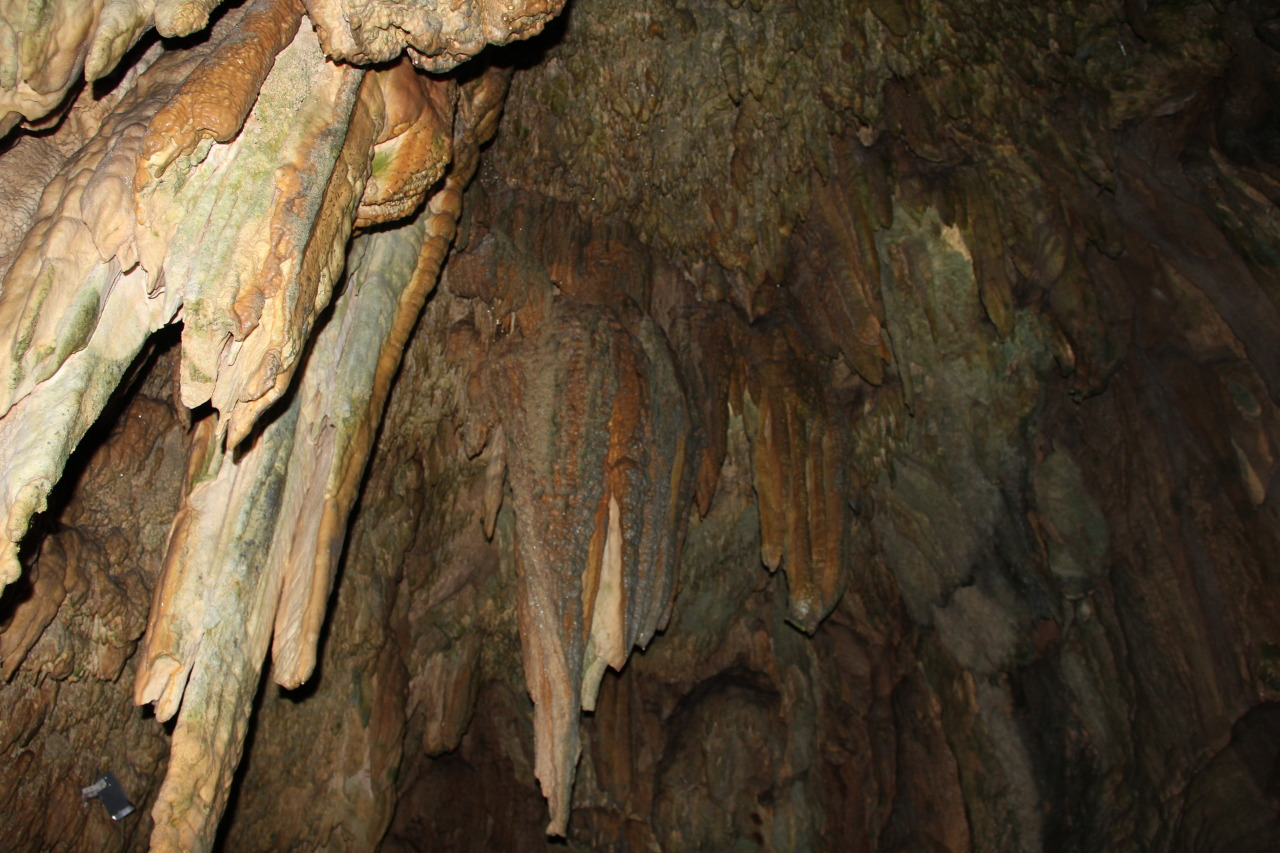
\includegraphics [width=0.3\textwidth]{../Bilder/Aegeri/16.jpg}}\quad
   \subfloat{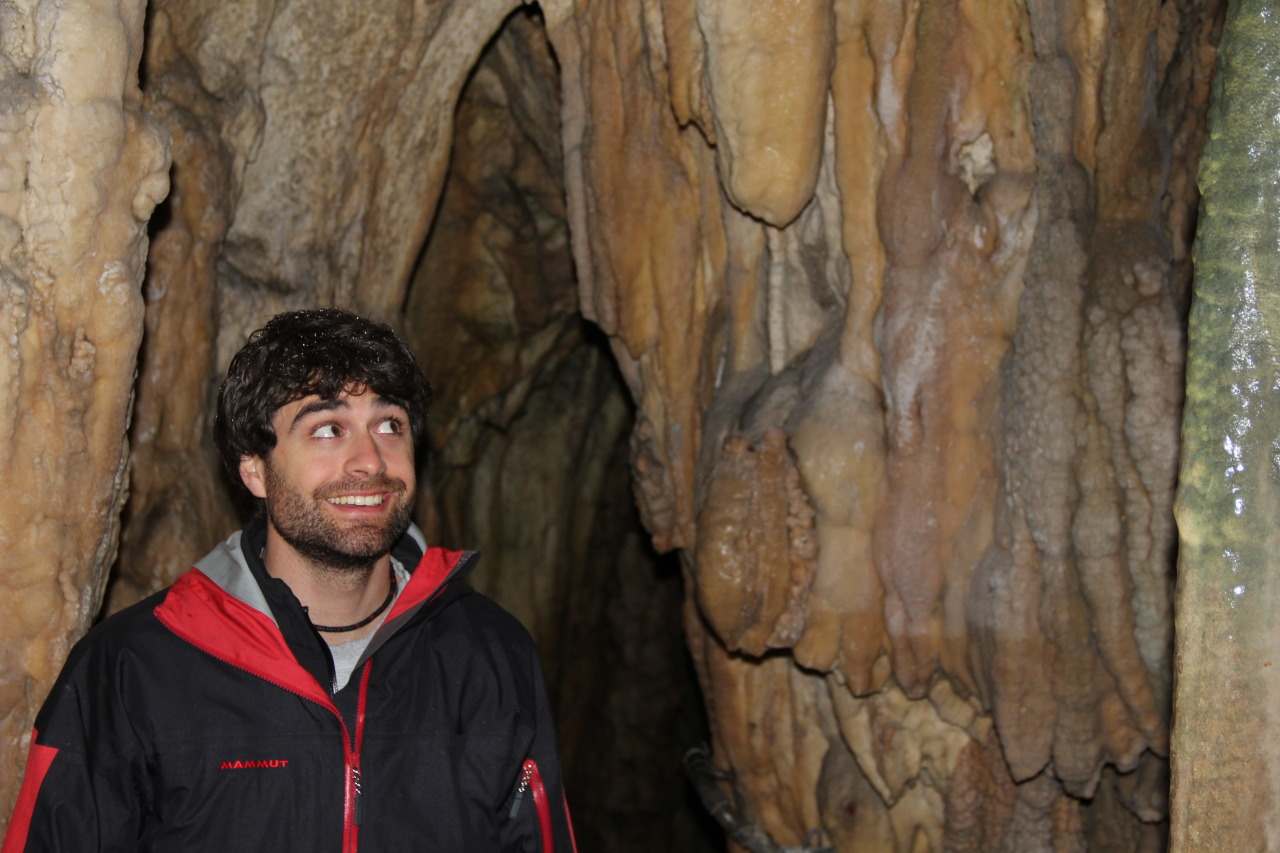
\includegraphics [width=0.3\textwidth]{../Bilder/Aegeri/18.jpg}}\quad
   \subfloat{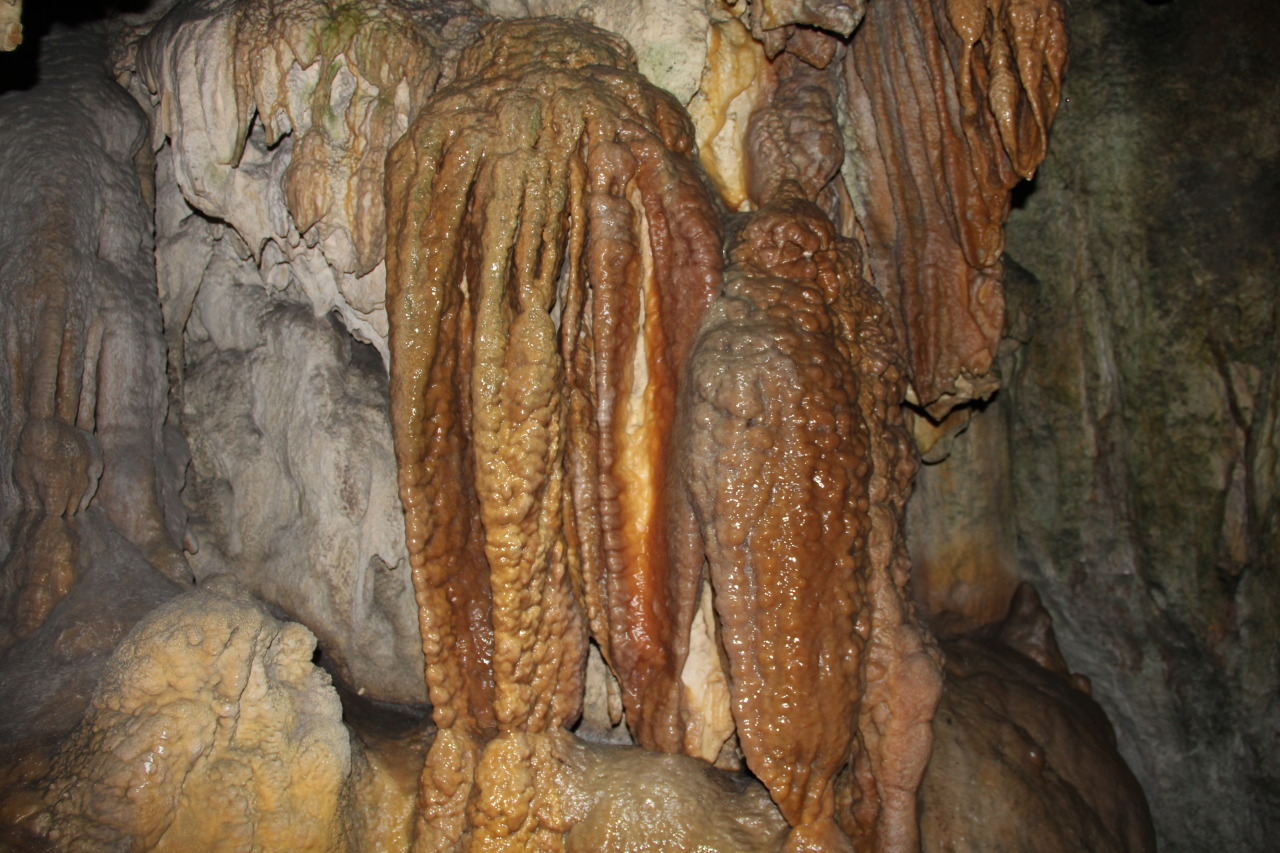
\includegraphics [width=0.3\textwidth]{../Bilder/Aegeri/23.jpg}}\quad
   \caption[In der H�llgrotte]{In der H�llgrotte}
\end{figure}

Die Fahrt zur�ck nach Hause verlief reibungsfrei aber immer noch bei starkem Schneefall.
Ein Wochenende welches uns unerwartet kaltes Wetter gebracht hat.
Eine spannende Erfahrung, welche wir jedoch noch so gerne mit 20�C Wetter getauscht h�tten.

\newpage
\section{Sommer 2012}
\subsection{31.07.2012 Die letzten Vorbereitungen}
Da unsere n�rdlichen Nachbarn mit der Lieferung von sehnlichst erwarteten Ersatzteilen in Verzug waren, musste unser Notnagel Tobi einspringen.
Zuverl�ssig wie eh und je konnte ich am Abend die ben�tigten Teile abholen.
Das Ganze noch Kurz im Bus eingebaut und der langen Fahrt sollte nichts mehr im Wege stehen.
Die Batterie, welche in letzter Zeit eher mit schwacher Leistung gegl�nzt hatte, konnte dank Garantie problemlos eingetauscht werden. (Danke Chantal)

\subsection{01.08.2012 Nutzlast?}
Der Tag stand ganz im Zeichen der Nahrungsaufnahme.
Der aufmerksame Beobachter k�nnte meinen, dass wir unsere K�rpereigenen Reserven f�r unsere Reise aufladen.
Jedoch war der Grund nicht die Angst vor einer drohenden Hungersnot, sonder der 1.August, Nationalfeiertag der Schweiz.
Also reingehauen, kann ja nicht schaden.
Trotzdem mussten die anstehenden Arbeiten noch erledigen werden.
Das Tanken kurz nach dem traditionellen Feuerwerk in Baden bescherte der Coop-Tankstelle einen fetten Benzinflecken.
Mein �bermut und meine Viel hilft viel Philosophie wurde bestraft.
Der �bergang von Tankstutzen zu Benzintank pr�sentiert sich leicht spr�de und der wertvolle Saft fand den Weg aus dem Bus zur�ck zur Tankstelle.
Gl�cklicherweise befindet sich das Leck in naher Distanz zum Tankdeckel.
So kam es, dass wir erst nach 11 Uhr unser wohlverdienter Sch�nheitsschlaf beginnen konnten.
Schon arg nahe am unsch�nen Weckerton, welcher uns um 04:30 f�r den Beginn der Reise aus den Federn holen sollte. 
Als erstes Ziel wollten wir m�glichst viele Kilometer hinter uns bringen, damit wir nicht jeden Tag Auto fahren m�ssen.
Unser zugegebenerma�en ambiti�se Ziel war: Rom.
Viele Wege f�hren nach Rom, doch wir werden nur einen ben�tigen.
Viele selbsternannte Kritiker und M�chtegern VW-Bus Kenner l�chelten �ber unser Vorhaben und streuten gezielt Zweifel.
Auch wir waren nach den j�ngsten Ereignissen nicht abgeneigt den allj�hrlichen TCS Beitrag zu bezahlen um f�r das allerschlimmste gewappnet zu sein.  

\begin{figure}[hbt]
    \centering
    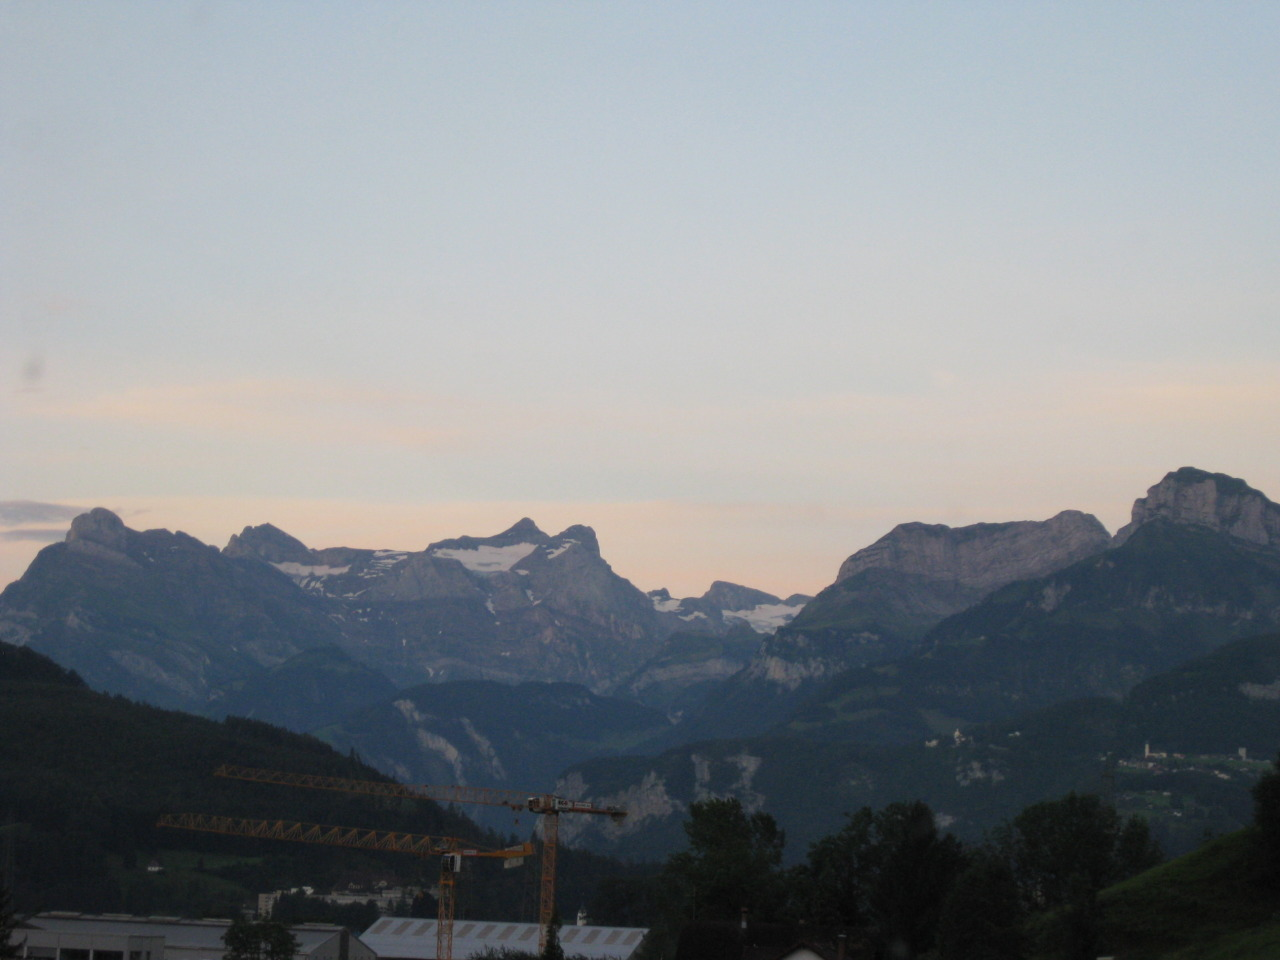
\includegraphics[width=\textwidth]{../Bilder/Sommer2012/1.jpg}
    \caption{Auf dem Weg in den S�den}
    \label{img:Sommer1}
\end{figure}

\subsection{02.08.2012 Es geht los}
Kurz nach 5 Uhr waren auch die letzten Ausreden, welche gegen eine Abfahrt gesprochen h�tten aus dem Weg ger�umt und wir machten uns auf den Weg gen S�den.
Schon fr�h fanden wir einen geeigneten LKW um uns in den Windschatten zu h�ngen und die Reise bei einem geringerem L�rmpegel zu absolvieren.
Der Berufsverkehr hielt sich in Grenzen und schon bald konnten wir unseren ersten Espresso an der Rastst�tte Gottardo Sud genie�en.
Kurz nach der ersten Pause wurde die Frage nach dem Fackel f�r die F�hr�berfahrt nach Kroatien leider negativ beantwortet.
Eine wilde Suche nach dem Best�tigungsmail auf dem Handy begann.
Wir entschlossen uns die n�chste Rastst�tte zu nutzen um mittels Laptop nach dem vermeintlich verloren gegangenen Mail zu suchen.
Die Suche f�hrte zu einem Treffer im SPAM Ordner, welcher einen Tag sp�ter automatisch gel�scht worden w�re.
Gl�ck gehabt. Weiter ging die Reise Richtung Italienischer Grenze.

Da Jack mittlerweile zum Liebling der Polizeikontrollen avanciert ist (Sind daran m�glicherweise die gr�nen Hibiskusbl�ten schuld?), waren wir auf den Grenz�bertritt gespannt.
Doch ganz im Stile echter Italienischer Staatsangestellten verbrachten die anwesenden Z�llner ihre Zeit lieber mit Sp�sse als mit Kontrollen.

Nach einer kurzen Phase der Verkehrs�berlastung um Mailand ging die Flotte Reise Richtung S�den ungebremst weiter.
Die Landschaft wurde viel zu selten durch interessante Aussichten gest�rt.
Dominierend waren Felder und Hochspannungsmasten.
Waren zu Beginn die Temperaturen noch angenehm, n�herte sich das Thermometer je l�nger je n�her der Zone ziemlich bis wahnsinnig warm.
Man konnte H�hnchen fettarm zubereiten, wenn man sie aus dem offenen Fenster h�lt.
Gerade in Mitten einer LKW Kolonne, welche sehr h�ufig (zu h�ufig) auftraten, war der Atem eines Heissluftf�hnes zu sp�ren.
Die lieben Lkws machten Chantal zu schaffen.
Gerade als sie den n�tigen Schwung f�r ein �berholman�ver gesammelt hatte, scherte der schl�frige Chauffeur mit seinem langen Gef�hrt Richtung unserer Spur.
Dieses Man�ver provozierte eine wahre Sammlung netter Ausdr�cke, welche in ihrer Rohform so im �ffentlichen Raum nicht abgedruckt werden sollten.

Endlich n�herten wir uns Rom und damit begann die Suche nach einer Bleibe.
Die elektronische Sammlung von Campingpl�tzen um Rom schlug uns zwei Favoriten vor.
Um �berhaupt dort hin zu kommen mussten wir den Westring von Rom befahren, welcher uns mit Stau und den dazugeh�rigen spannenden �berholman�ver begr��te.
Der erste Angesteuerte Campingplatz war closed.
So jedenfalls die Aussage eines beim Eingang abgestellten Typen.
Wir sollen es bei einem anderen Versuchen.
Das taten wir und wir hatten Gl�ck.
200 Meter vom Strand entfernt fanden wir kurz vor 19:00 unser erster Standplatz.
Nach dem hastigen Einrichten stand einem Bad im Meer nichts mehr im Weg.

Auf dem R�ckweg sahen wir ein sch�ne Restaurant am Meer, welches aber alles andere als gut besucht war.
Wir beschlossen, unser Gl�ck nach dem Frischmachen dort zu suchen.
Nat�rlich war um 22:00 das lokal von Einheimischen �bersp�lt worden.
Ein kurzer Blick �ber die Strandpromenade bescherte uns Gewissheit, dass dieses Lokal das einzig brauchbare zu sein scheint.
Nur hier waren Autos geparkt.
So mussten wir uns mit dem Campingrestaurant begn�gen.
Wir wurden keinesfalls Entt�uscht.
Chantal stellte die Spaghetti Pesto in Rekordzeit herunter und auch ich musste mich keinesfalls hinter der Pizza verstecken.
Die eigentlich ganz fleissige Bedienung musste jedoch genau in der Phase, in der die M�cken wieder ein prominentes Opfer gefunden haben, eine, nein zwei Rauchpausen einlegen.
Kurz vor 24:00 war der erste lange Tag unserer Reise Geschichte.

\begin{figure}[h]
   \centering
      %\subfloat[CAPTION]{BILDERCODE}\qquad
   \subfloat{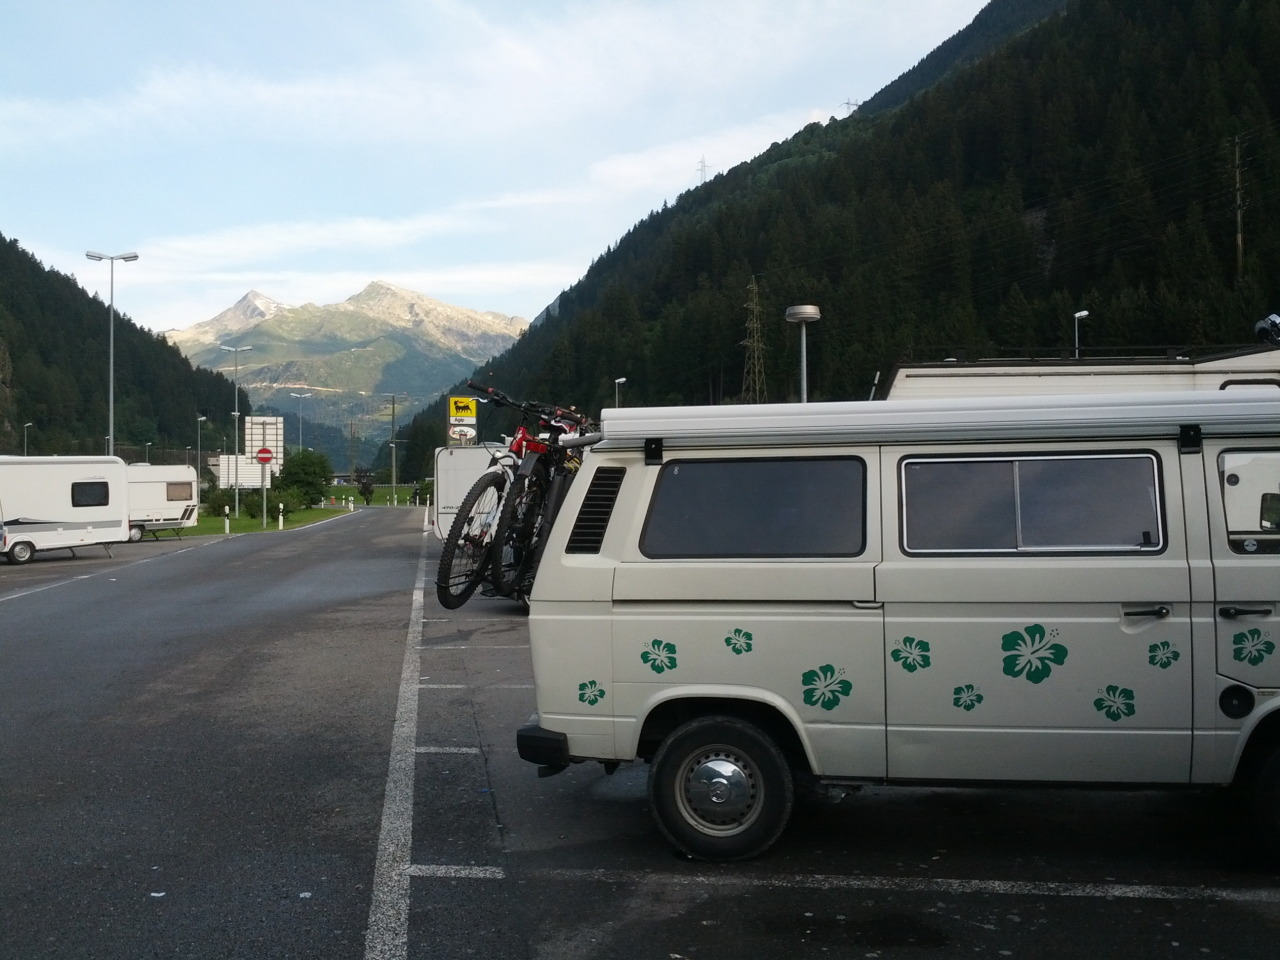
\includegraphics [width=0.3\textwidth]{../Bilder/Sommer2012/2.jpg}}\quad
   \subfloat{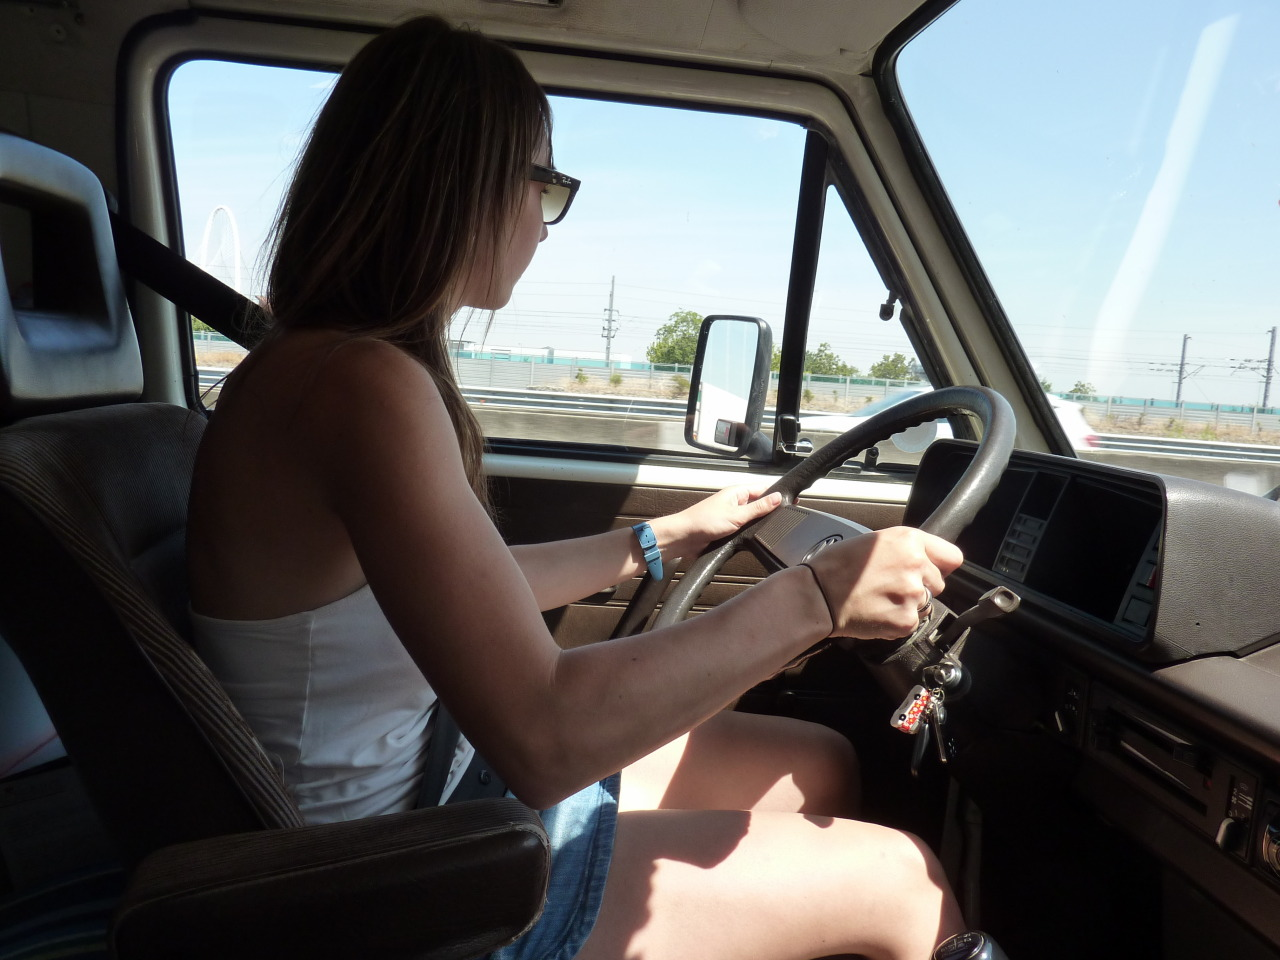
\includegraphics [width=0.3\textwidth]{../Bilder/Sommer2012/3.jpg}}\quad
   \subfloat{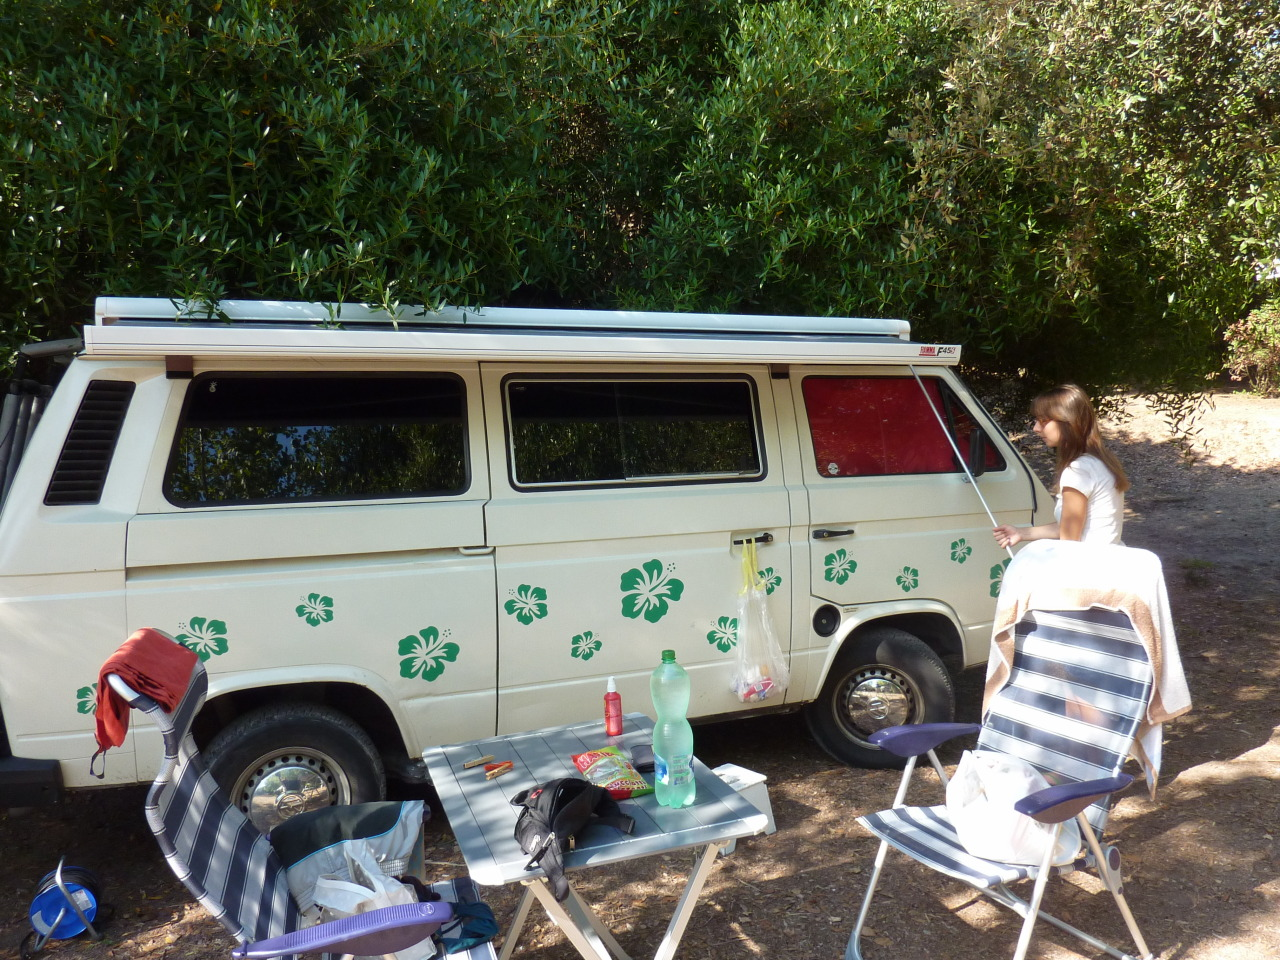
\includegraphics [width=0.3\textwidth]{../Bilder/Sommer2012/5.jpg}}\quad
   \caption[Weg und Ankunft in Rom]{Weg und Ankunft in Rom}
\end{figure}

\subsection{03.08.2012 Roma bei gef�hlten 220� C}
Durch die geschickte Platzwahl konnten wir wunderbar im Schatten aufwachen.
Die Temperaturen waren auf ein angenehmes Mass gesunken w�hrend der Nacht.
Doch was bewegt sich da? AMEISEN.
Nicht gerade wenige nutzten unseren Bus als eine Art �bergrosse Treppe um von einem Baum auf den Boden zu kommen.
Bei dieser Gelegenheit betrachteten diese Biester auch gerade noch unsere Innenraumaustattung.
Frechheit sowas.
Umparken war angesagt.
Mittels wilder Rangierman�ver ohne R�cksicht auf Flora und Fauna war der neue Standplatz inert Minutenfrist erreicht.
Anti-Brumm scheinen die vielbeinigen Plaggeister nicht zu m�gen.
Jedenfalls veranstalten sie bei jedem Spr�hangriff einen wilden Tanz und fallen wie Reife Pflaumen vom Bus.
Das Fr�hst�ck wurde trotzdem genossen.

Nach kurzer Recherche verwarfen wir die verwegene Idee Rom vom Campingplatz aus mit dem Velo zu erkunden.
Weit �ber 25 km Distanz und Aussicht auf einen eher warmen Tag machten uns diese Entscheidung leicht.
�V f�hrt von hier bis ins Stadtzentrum und diese Transportmittel nutzen wir auch um in ca 1 Stunde neben dem Kolosseum aus dem Untergrund in der Hitze aufzutauchen.
Naja, so kolossal sah diese Ruine jetzt nicht gerade aus.
Auch das Forum Roman haute uns nicht aus den Socken oder �hm Sandalen.
Mit R�mersandalen wollte ich durch das Forum Roman schlendern und die Latein-stunden der Bezirksschule wieder aufleben lassen: Ave Ceasar.
.Salve Titus.
.;) aber die Ruinen des Forums sahen gar nicht einladend aus; sie glichen eher einem Friedhof als einer spektakul�ren und historischen St�tte.
So machten wir uns auf den Weg zu der spanischen Treppe, die bekannteste Treppe der Welt.
Aber wo war diese? Obwohl sie ziemlich gross ist, hatten wir M�he sie zu orten.
Da die Geographin die Treppe neben dem Forum Roman vermutete, sie aber �berhaupt nicht dort war, wurde aus jeder Treppe rings um das Forum Roman die spanische Treppe ;) So haben wir viele Treppen erklommen und uns immer gedacht: die ist aber nicht so imposant wie auf dem Bild.
Nach einigen Fehlversuche haben wir dann doch herausgefunden, dass wir auf der falschen F�hrte sind und haben einen neuen Anlauf genommen.

\begin{figure}[h]
   \centering
      %\subfloat[CAPTION]{BILDERCODE}\qquad
   \subfloat{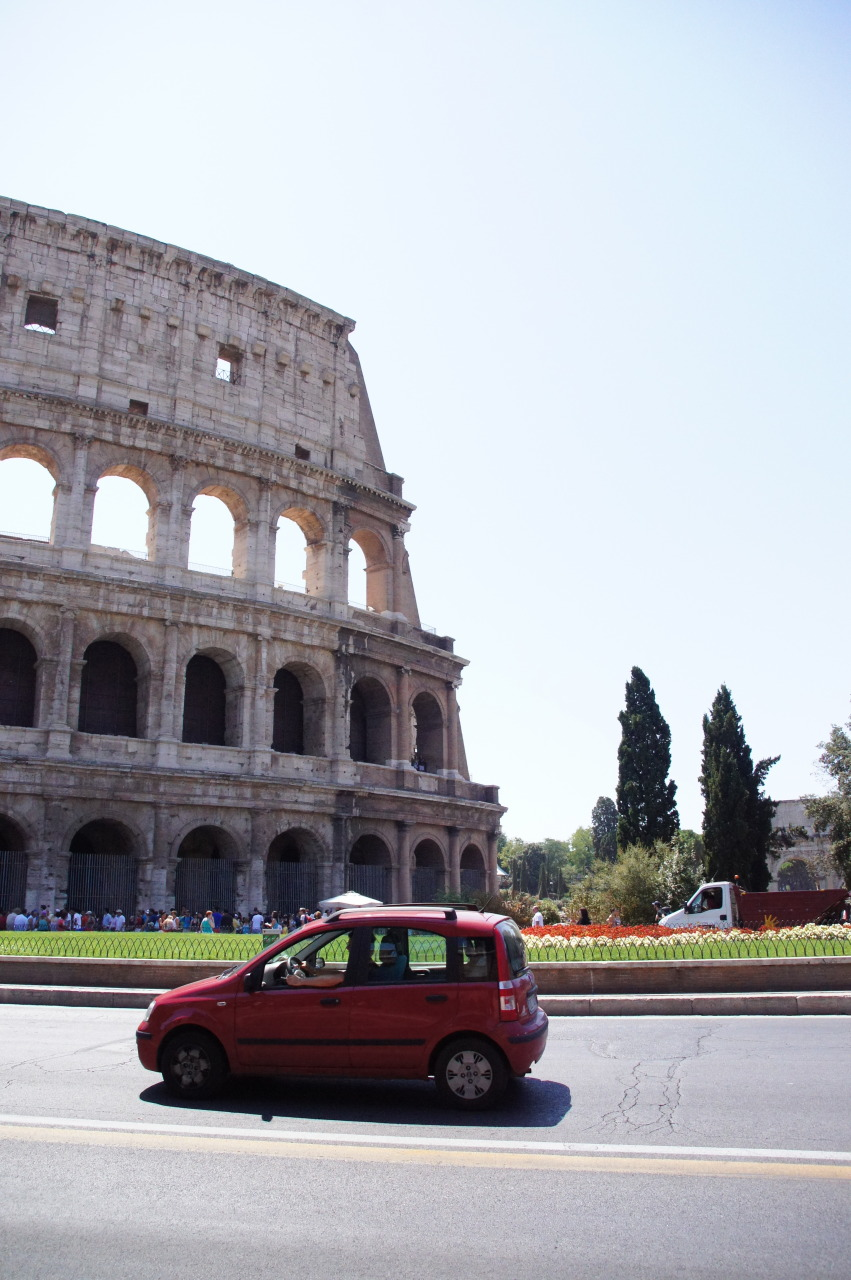
\includegraphics [width=0.3\textwidth]{../Bilder/Sommer2012/6.jpg}}\quad
   \subfloat{
\includegraphics [width=0.3\textwidth]{../Bilder/Sommer2012/7.jpg}}\quad
   \subfloat{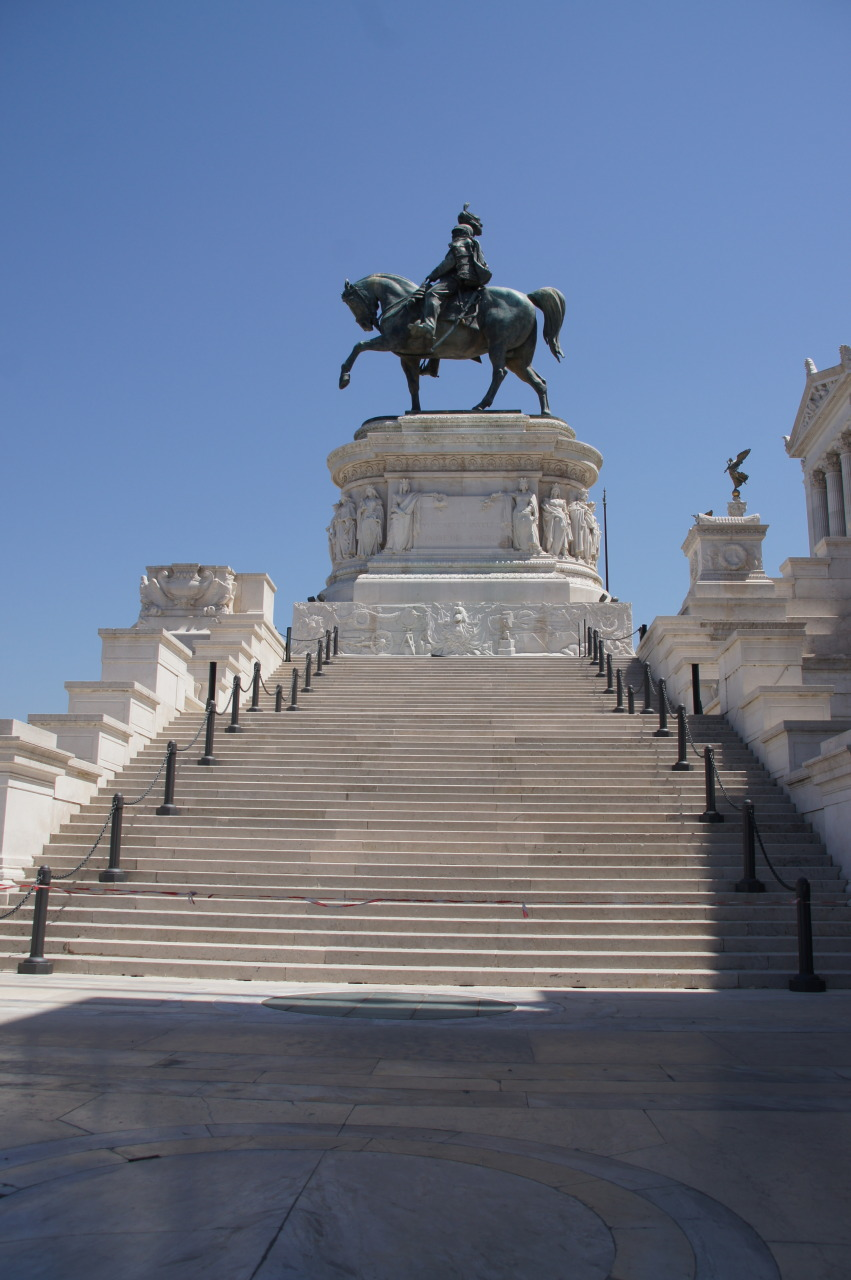
\includegraphics [width=0.3\textwidth]{../Bilder/Sommer2012/8.jpg}}\quad
   \caption[Sightseeing in Rom]{Sightseeing in Rom}
\end{figure}

Und da liefen wir direkt ins Judenviertel; j�dische Touristeninformation, Judensterne und koscher Essen gab es �berall und das direkt neben dem Vatikan.
Sogar koscher Kebab gab es.
Dann meldete sich der Hunger.
Wir g�nnten uns eine Pizza und Bruschetti, was aber eher eine schlechte Idee war.
Von der brennenden Sonne verging uns schnell der Hunger und wir k�mpften um jeden Bissen.
Nur mit viel Wasser und Cola konnten wir fast alles herunterschlingen.
Die Konsequenz daraus war, dass unser Magen bei der Hitze das Essen nicht so gut ertrug und wir uns nach dem Essen schlechter f�hlten als bevor.
Steff k�mpfte mit der Hitze und der Pizza im Magen.
So marschierten wir zur spanischen Treppe, die wir schlussendlich auch fanden und welche immer noch nicht so spektakul�r wie auf dem Bild im Reisef�hrer aussah.
Nach einem Drink (viiiiel Wasser;)) machten wir uns dann auch schon auf den Heimweg.
Wir mussten uns eingestehen, dass ein Stadtbesuch bei dieser Hitze nicht so angenehm ist.
Im Camping angekommen, freuten wir uns auf die Dusche und einen gem�tlichen Abend.
Zum Nachtessen gab es feine Chilli-Oliven, Chips und Tomatensalat.
Mehr vertrug unser gestresste Magen nicht;) Wir lasen vertieft in unseren B�chern mit sch�ner Musik (Campingband) im Hintergrund.

\subsection{04.08.2012 Relaxxxxx}
Dieser Tag stand ganz im Zeichen des Faulenzen.
Wir schliefen aus und auch die aggressiven Ameisen konnten uns nicht fr�her aus den Federn holen.
Danach war ein Tag am Strand angesagt.
Mit Hilfe von Sonnenschirm und Wind konnte es man problemlos einen ganzen Tag am Strand aushalten.
Lesen und Faulenzen...
Am Abend besuchten wir das Restaurant am Strand, welches am ersten Tag hoffnungslos �berlaufen war.
Dieses Mal reservierten wir jedoch.
Die Servierd�se konnte mir alles andrehen, jedenfalls sah das Chantal so und darum wurde aus dem Znacht ein gediegenes Mahl.
Erst sp�t am Abend kehrten wir zu unserem Bus zur�ck wo wir m�de in Federn fallen wollten.
Jedoch machte uns ein hinterlistiges Sandkorn einen Strich durch die Rechnung.
Irgendwie verfing sich dieses Korn in einem Auge und blieb dort hartn�ckig die ganze Nacht, was zu einer eher ungem�tlichen Nacht f�hrte

\begin{figure}[hbp]
    \centering
    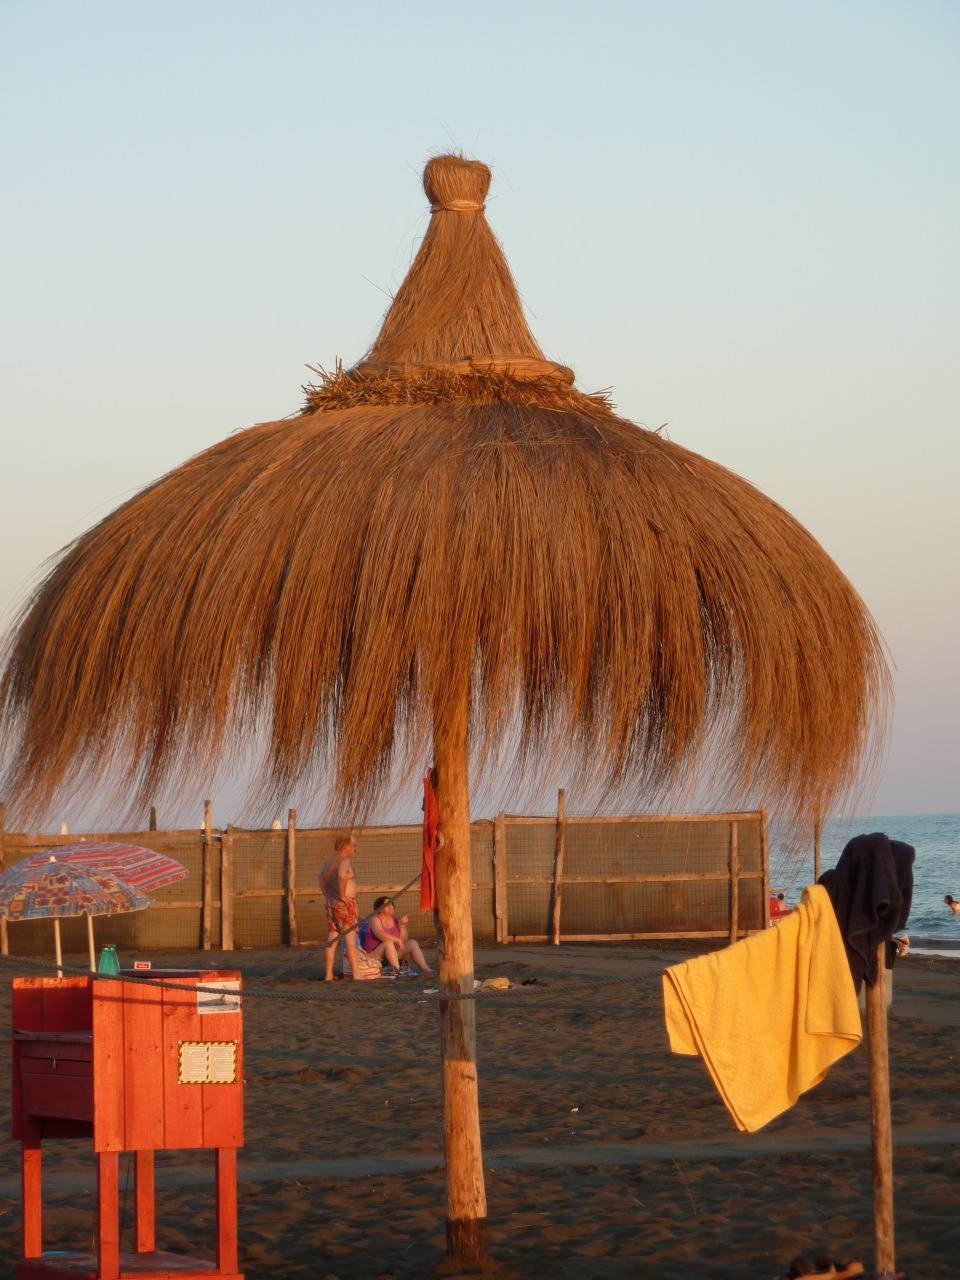
\includegraphics[width=\textwidth]{../Bilder/Sommer2012/4.jpg}
    \caption{Am Strand in Rom}
    \label{img:Sommer2}
\end{figure}

\subsection{05.08.2012 Je s�dlicher ,desto tsch tsch}
Der Morgen kam viel zu fr�h und beide Busfahrer hatten irgendwie einen komischen Magen.
So fiel das Fr�hst�ck sehr sp�rlich aus und schon bald fingen wir an unsere 7 Sachen im Bus zu verstauen.
Um 10 Uhr war Abfahrt und der Weg f�hrte Richtung Vieste.
Es wurde zu einer �u�erst ungem�tlichen Fahrt, welche nur ein gutes Ende nahm, weil gewisse Tabletten aus Armeebest�nde den Weg in unsere M�gen fanden (Besten Dank dem Dr.  Sponsor).
Wir wollten die Fahrt schon aus gesundheitlichen Gr�nden unterbrechen, bissen uns dann aber bis nach Peschici durch.
Auch Jack musste das erste Mal so richtig leiden.
Die Temperatur blieb zwar stets im gr�nen Bereich, jedoch wollte er mit Hilfe des Standgases nicht mehr unbedingt seinen Dienst tun.
Unser neu montiertes Endrohr hing nur noch an einer Schraube statt an deren Drei.
Draht schafft hier Abhilfe (hoffentlich) Auch um 20:00 ist hier das Thermometer noch auf den oberen Etagen unterwegs und denkt nicht einmal daran in angenehmere Regionen zu sinken.
Das wird eine feucht-(fr�hliche) Nacht.

\begin{figure}[H]
    \centering
    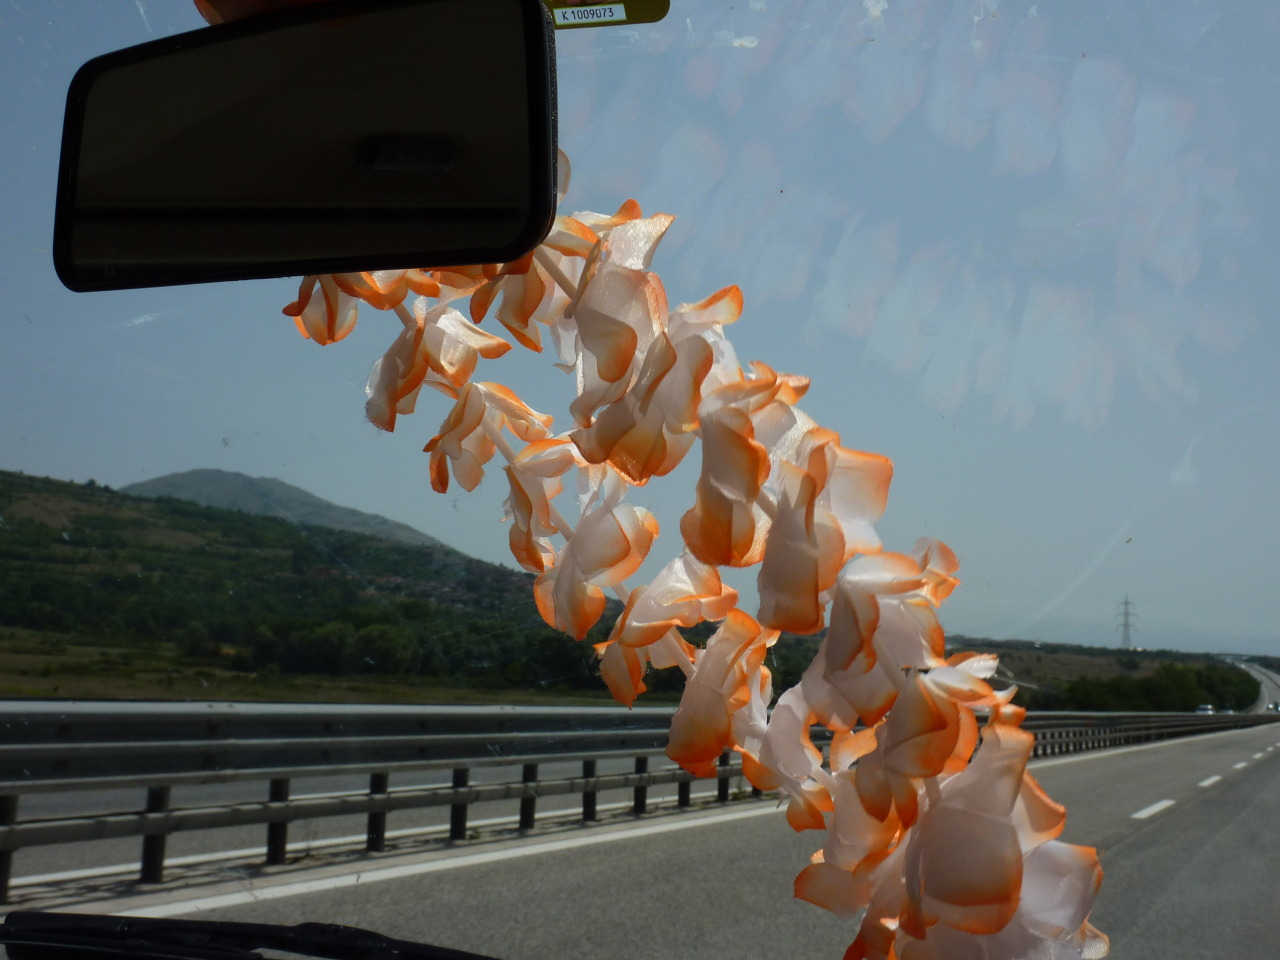
\includegraphics[width=\textwidth]{../Bilder/Sommer2012/11.jpg}
    \caption{Im Glutofen unterwegs}
    \label{img:Sommer3}
\end{figure}

\subsection{06.08.2012 Jack Sparrow alias Pepito}

\begin{wrapfigure}{R}{0.45\textwidth} 
  \begin{centering}
    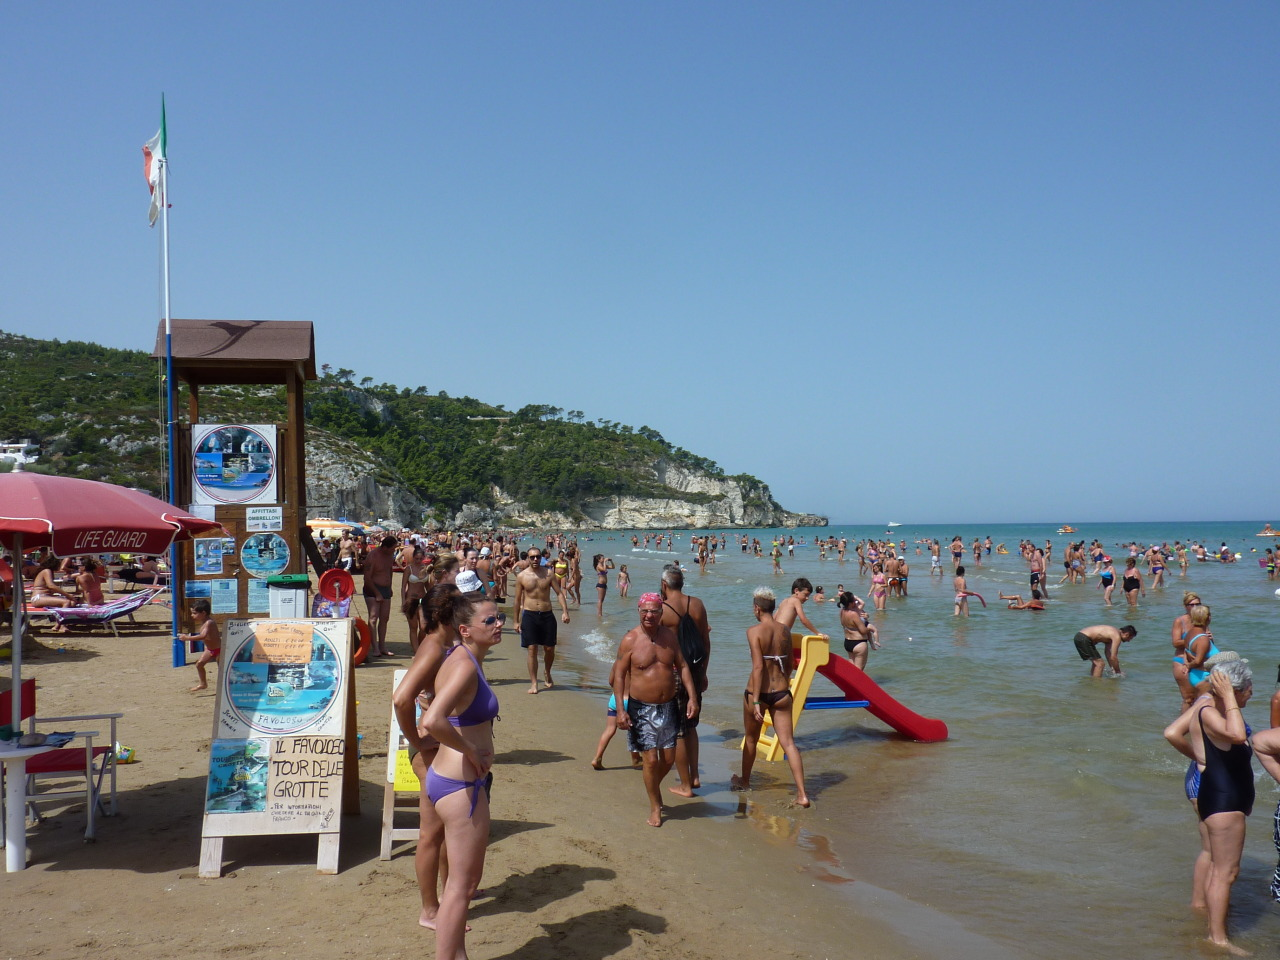
\includegraphics[width=0.4\textwidth, height=5cm, keepaspectratio]{../Bilder/Sommer2012/13.jpg}
    \caption{Action am Strand}
  \end{centering}
\end{wrapfigure} 

Die Nacht war trotz �blen Vorahnungen gar nicht so �bel.
Chantal jubelte schon fr�h am Morgen dar�ber, dass ihr hartn�ckiges Sandkorn verschwunden war.
So begann sie kurz nach 9 mit der Suche nach dem Mercato.
Wieso in aller Welt ist dieser Laden in der H�chstsaison geschlossen? Nach kurzer Absprache sattelten wir die Velos und begannen mit der Suche nach Nahrungsmittel.
Eine Tafel die mit �u�erst optimistischen 20 Meter Distanz zum Supermercato wirbt wurde rasch gefunden so wie auch der Laden der 300 Meter von der Tafel entfernt war.
Das Fr�hst�ck fiel reichhaltig aus.
Das Ameisenproblem waren wir gl�cklicherweise los.
Trotzdem machte sich jedes Brotkorn das auf den Boden fiel sofort auf den Weg Richtung Nesteingang.
Die Ameisen hier sind mindestens doppelt so gross wie in Rom und Gott sei Dank nicht an der Inneneinrichtung interessiert.
Der Weg zum Strand war kurz und schon bald waren die Liegest�hle in Beschlag genommen.
Doch was st�rte da mein sensibles Ohr? Gustavo Lima! Mindestens 50 Italiener in aller Form und Alter absolvierten eine Art Fitnesstraining am Strand.
Nach einer halben Stunde war Ruhe f�r ca.  10 Sekunden bevor der n�chste Strandabschnitt mit anderen beknackten Spielchen anfing.
Schon bald begann ich mich auf die Suche nach ein wenig Ruhe und wurde schnell f�ndig.
Ein Typ, der Jack Sparrow alt aussehen l�sst bot mir zwei Liegest�hle an, welche auch sofort besetzt wurden, nach dem ich Chantal geholt habe.
Den Rest des Tages verbrachten wir mit Faulenzen und Baden.

Am Abend stand dagegen Fitness auf dem Speiseplan... Die H�user schmiegen sich leicht erh�ht an die H�gel und genau dort wollten wir mit dem Velo hin.
Um 21 Uhr waren die Temperaturen langsam ertr�glich und wir machten uns auf den Weg, welchen wir Schweissgetr�nkt zur�cklegten.
Alle L�den hatten noch offen, dieser Umstand und die sch�nen, zahlreichen engen Gassen l�sten Gl�cksgef�hle bei Chantal aus.
Einen Teller Orechiette al Peschici f�hrten bei mir zu einer �hnlichen Reaktion.
Die Abenteuerliche Abfahrt, welche wir im Schein der Stirnlampe unter die R�der nahmen war die letzte Aktion an diesem sch�nen Tag.

\subsection{07.08.2012 Slow down..take it easy}
Heute war wieder ein Strandtag angesagt.
Doch zuerst wollten wir nochmals das sch�ne St�dtchen Peschici bei Tageslicht betrachten.
Um halb 9 Uhr machten wir uns mit dem Velo auf den Weg und hatten sogar noch Gl�ck, da der Weg weit weit hinauf teilweise im Schatten lag.
Oben angekommen streiften wir gem�tlich durch die herzigen Gassen und genossen die sch�ne Aussicht auf das t�rkisfarbene Meer.
Wir trafen sogar die Frau an, bei welcher ich gestern eine sch�ne Ledertasche geschenkt bekommen habe;) In einem Restaurant konnten wir einen feinen Kaffee geniessen, feine Croissant (eins mit Nutella;)) essen und sogar Flieger beobachten, welche im Meer Wasser f�r einen Brand hinter den H�geln holte.
Da war einer seeehr gl�cklich �ber dieses Spektakel :D Dann fetzten wir mit den Velos den Hang hinunter, gingen in den Supermercato, wo wir einen Sonnenschrim fanden, machten einen Zwischenstop im Camping und schlenderten dann zum Strand (Bei dieser Hitze kann man nicht viel schneller laufen als zu schlendern) Am Strand versuchten wir unser frisch gekauften Sonnenschirm festzumachen, was sich aber eher als schwierig herausstellte.
Der Sand war ziemlich hart.
Nach kurzer Zeit kam uns eine Italienerin zur Hilfe und zeigte uns, wie man das macht.
Endlich konnten wir uns hinlegen, sonnen, lesen, faulenzen und baden.
Heute war es sogar aushaltbar an der Sonne (f�r einige;)), da ein angenehmer Wind wehte.
Den Abend verbrachten wir mit Trinken (Bier, Campari und Wein;)) und Essen.
Hmmm ich freue mich auf die Orechiette!  

\begin{figure}[h]
   \centering
      %\subfloat[CAPTION]{BILDERCODE}\qquad
   \subfloat{\includegraphics [width=0.3\textwidth]{../Bilder/Sommer2012/16.jpg}}\quad
   \subfloat{\includegraphics [width=0.3\textwidth]{../Bilder/Sommer2012/18.jpg}}\quad
   \subfloat{\includegraphics [width=0.3\textwidth]{../Bilder/Sommer2012/21.jpg}}\quad
   \caption[Peschici]{Peschici}
\end{figure}

\subsection{08.08.2012 Vieste}

\begin{wrapfigure}{L}{0.45\textwidth} 
  \begin{centering}
    \includegraphics[width=0.4\textwidth, height=5cm, keepaspectratio]{../Bilder/Sommer2012/22.jpg}
    \caption{Vieste}
  \end{centering}
\end{wrapfigure} 

Um 12:00 mussten wir sp�testens den Campingplatz verlassen haben.
Eigentlich kein Problem, wenn da nicht die sehr aktiv anstehenden Italiener w�ren.
Nur aus Mitleid der Bedienung kam ich an die Reihe.
Normalerweise schrie bei der Frage: "`Wer ist der n�chste?"' immer eine als klassische Operns�ngerin ausgebildete Italienerin aus der dritten Reihe und bekam ihre 2 Kilogramm Mortadella vor mir.
Beim Aufr�umen fanden wir noch gewisse �berreste einer roten Fl�ssigkeit, die sich in alle Ritzen unseres Tisches eingenistet hat.
B�se Zungen behaupten es k�nnte dieselbe berauschende Fl�ssigkeit sein, welche zum umfallen des Weinglases verf�hrte (g�ll, Chantal :)) Nach dem Morgenessen waren unsere Habseligkeiten dann schnell verstaut und um 11:30 machten wir uns auf den Weg dem Meer entlang Richtung Vieste.
Das Navi war nat�rlich wieder �usserst optimistisch mit der Zeitangabe: 30 Min.
Die Fahrt war wundersch�n und schon nach einer Stunde erreichten wir Vieste und den angepeilten Campingplatz.
Dieser war sich jedoch zu Schade uns f�r 2 N�chte aufzunehmen.
Absteigende m�ssen mindestens eine Woche dort bleiben.
Nicht mit mich.
Der n�chste war dann schnell gefunden und bot zwar viel Schatten, daf�r auch sehr wenig Platz.
Egal, hauptsache sofort an den Strand, an dem ich meine zugegebenerma�en abgeschauten Sonnenschirm Eingrabtechnik stolz den nicht anwesenden Badeg�ste pr�sentierte Badeg�ste.
�ber die Mittagsstunden fl�chten diese Weicheier und Beckenrandschwimmer immer zur�ck zu ihren klimatisierten Wohnungen und Wohnw�gen.
Nur wir, sonnenverw�hnten Schweizer halten es am gl�henden Strand aus.
Der Abend n�herte sich immer mehr und meinen Versuch die Luftmatratze ohne Pumpe auf 2 Bar zu bringen scheiterten kl�glich.
An dieser umgewandelter PET Flasche befanden sich extrem effiziente Ventile.
Luft geht nicht rein und auch nicht wieder raus.
Die 3 Liter die ich in m�hsamer Arbeit in die Matratze gepresst hatte, konnte ich nun nicht wieder ablassen.

Endlich ging es Richtung Vieste.
Die ersten Schuhgesch�fte wurden durch Chantal gepl�ndert, genauso wie Attila die westliche Welt heimsuchte.
Das Restaurant direkt am Meer sorgte f�r einige Kritik (meinerseits), trotz allem war es ein sehr gelungener Abend in einer �usserst sch�nen Stadt.
Bei der Ankunft auf dem Zeltplatz durften wir noch den Kl�ngen sehr schlechter Karaokes�nger lauschen, die fehlendes Talent geschickt mit Lautst�rke zu kompensieren versuchten.
Die Sonne, die W�rme und ein wenig Campari sorgten jedoch f�r einen sehr tiefen und schnellen Schlaf trotz wildem Vibrieren von stark ge�lten Stimmb�ndern.

\begin{figure}[h]
   \centering
      %\subfloat[CAPTION]{BILDERCODE}\qquad
   \subfloat{\includegraphics [width=0.3\textwidth]{../Bilder/Sommer2012/23.jpg}}\quad
   \subfloat{\includegraphics [width=0.3\textwidth]{../Bilder/Sommer2012/25.jpg}}\quad
   \subfloat{\includegraphics [width=0.3\textwidth]{../Bilder/Sommer2012/31.jpg}}\quad
   \caption[Rundgang durch Vieste]{Rundgang durch Vieste}
\end{figure}
 
\subsection{09.08.2012 Besuch der Altstadt}
Die weiteren Berichte werden sicherlich negativ beeinflusst von einem Ereignis, welches sich am 11.08.2012 ereignet hat.
Die folgenden zwei Tage waren garantiert lustiger und sch�ner als hier Beschrieben:
Ein weiteres Mal stiegen wir auf unsere Drahtesel und Radelten schon vor dem Mittag Richtung Vieste.
Dort angekommen starteten wir eine weitere Runde Sightseeing.
Viele Bilder wurden geschossen und von den n�chsten Restaurierungsobjekten getr�umt.
Den Kaffee nahmen wir bei einem Deutschsprechenden Italiener ein und genossen die Stadt bis in die Abendstunden.
Italienisch angehaucht suchten wir den Strand erst um 18:00 Uhr auf und genossen die angenehmen Abendstunden am Wasser.
Chantal konnte sich an der am Strand abgehaltenen Cha-Cha-Cha Tanzlektion kaum sattsehen.
Zur�ck auf dem nahegelegenen Camping bereiteten wir uns ein gem�tliches Abendessen vor und fielen �usserts zufrieden auf die warmen Matrazen.

\begin{figure}[H]
    \centering
    \includegraphics[width=\textwidth]{../Bilder/Sommer2012/30.jpg}
    \caption{Vespa in Vieste}
    \label{img:Sommer4}
\end{figure}

\subsection{10.08.2012 Fahrt nach Monopoli}
Auch hier mussten wir bis um 12:00 den Campingplatz verlassen haben.
Chantal besorgte das Morgenessen und ich verbrachte die Zeit mit der Vorbereitung f�r die Abfahrt.
Stolz verk�ndete ich nach getaner Arbeit eine neue Rekordzeit f�r die Aufr�umarbeiten.
Schnell gezahtl und ab ginge es auf den wundersch�n verschlungenen K�stenstra�en Richtung S�den.
Das n�chste Ziel war Trani.
Das wir mit einem kurzen Umweg erreichten.
Ein Parkplatz war schnell gefunden und die Parkanlage am Hafen wusste mehr als zu �berzeugen.

\begin{figure}[H]
   \centering
      %\subfloat[CAPTION]{BILDERCODE}\qquad
   \subfloat{\includegraphics [width=0.3\textwidth]{../Bilder/Sommer2012/38.jpg}}\quad
   \subfloat{\includegraphics [width=0.3\textwidth]{../Bilder/Sommer2012/40.jpg}}\quad
   \subfloat{\includegraphics [width=0.3\textwidth]{../Bilder/Sommer2012/41.jpg}}\quad
   \caption[Trani]{Trani}
\end{figure}

Ganz im Gegenteil zur Altstadt.
Als Entschuldigung muss hier aufgef�hrt werden dass zwar Siesta war, trotzdem glich das ganze einer Geisterstadt.
Einzelne Touristen schlurften durch die Gassen, alles andere war leer.
Eine Bar, welche ge�ffnet hat war nicht auszumachen.
Schlussendlich nahm uns ein Restaurant auf, bei dem sich die Bedienung �ber unsere sehr begrenzte Bestellung wunderte.

\begin{figure}[H]
    \centering
    \includegraphics[width=0.5\textwidth]{../Bilder/Sommer2012/43.jpg}
    \caption{An der K�ste bei Monopoli}
    \label{img:Sommer4}
\end{figure}

Nach dem der Bus wiedergefunden war, ging es weiter auf der SS 16 Richtung Bari/Brindisi.
Der Verkehr um Bari verhie� nichts positives f�r die baldige Wiederkehr am n�chsten Dienstag.
Der Reisef�hrer versprach schon keine Anh�ufung von Campingpl�tzen mehr und tats�chlich machten sich die begehrten Abstellpl�tze �u�erst rar.
Bei einem ersten kurzen Besuch von Polignano al Mare konnten wir keinen Campingplatz ausfindig machen.
4 km s�dlich von Monopoli hatten wir dann mehr Gl�ck.
San Stefano nahm uns in Empfang.
Die Einweisung auf den Platz nahm ein �bereifriger Ciao fahrender Platzgehilfe vor.
Wie wurden in Mitten von Dauercamper platziert.
Als ich den Versuch unternahm Jack auf dem Platz zu wenden, kam er mit lautem Zweitaktgeknatter angebraust und wies uns wild fuchtelnd vermutlich auf irgendetwas hin.
Wir verstanden nur das wir den Bus wieder drehen mussten.
Jedoch reichte so unsere Kabelrolle nicht bis zur n�chsten Elektrizit�t spendenden Pfosten.
Genau in diesem Augenblick durchzog es mich wie vom Blitz getroffen.
Ich hatte in Vieste den Adapter auf die lustigen Euro Stecker stecken gelassen.
SHIT, so viel zu der Bestzeit im Aufr�umen.
Ohne Strom kein K�hlschrank, kein
... und so weiter.
Ich h�tte mich schlagen k�nnen.
Der Besuch am Camping eigenen Strand bes�nftigte die Gem�ter wieder.
Pl�ne f�r eine Neubeschaffung wurden gemacht und Routen f�r das Velo nach Monopoli verglichen.
Ab ging es.

Die Stadt war wundersch�n von einer hellen Stadtmauer einges�umt.
Schmuckgesch�fte lockten und schon bald trafen wir auf dem Hauptplatz ein um einen gem�tlichen Ap�ro zu geniessen.
Noch schnell eine Flasche Wein gekauft und zur�ck ging es mit der Suche nach unseren Fahrr�dern.
Die Fahrt verlief durch absolute Dunkelheit und nur unsere Stirnlampen und das Velolicht verhalfen uns zu einer eingeschr�nkten Sicht auf die Strasse.
Auf dem Campingplatz angekommen wehte uns ein starker Wind entgegen.
Keine Chance auf ein gem�tliches Kochen vor dem Bus.
Also die "`K�che"' im Bus montiert und nach kurzer Zeit wurde das Abendessen serviert.
Noch kurz einen Film auf dem Laptop angeschaut und dann friedlich wurde friedlich einged�st.

P.S. Der Wein blieb an diesem Abend unangetastet. Ger�chten zu Folge war der Ap�ro daran Schuld.

\subsection{11.08.2012 Wundersch�ner Tag der am Abend leider eine sehr negative Wendung nahm.}
Das ist er also nun, unser Schicksalstag. 
Aber zuerst vorne Angefangen: Nach dem Morgenessen und dem Aufsuchen des Mercato (Eher eine Bar als ein Mercato... anyway) begaben wir uns ans Meer.
Leider war der Aufenthalt dort zeitlich begrenzt, da die augenscheinlich strenge Campingleitung mit Ciao-betriebenen Hilfssheriff, eine Fahrverbotszeitzone eingerichtet hat.
Ab 13:30 bis 16:00 war jeglicher Verkehr untersagt.
Jack machte schon bei den wilden Rangierversuchen mit seinem lockeren Auspuff auf sich aufmerksam und so versuchten wir wenn immer irgendwie m�glich uns an die Spielregeln zu halten.
Am Strand war der Kindergarten los.
Chantal am�sierte sich k�niglich �ber das wilde Treiben.
Andere verlie�en fluchtartig den Tatort.

\begin{wrapfigure}{L}{0.45\textwidth} 
  \begin{centering}
    \includegraphics[width=0.4\textwidth, height=5cm, keepaspectratio]{../Bilder/Sommer2012/54.jpg}
    \caption{Polignano al Mare}
  \end{centering}
\end{wrapfigure} 

Kurz nach 13:00 Uhr machten wir uns auf den Weg mit Sack und Pack um Polignano einen Besuch abzustatten.
Der Reisef�hrer versprach einen Parkplatz im Norden der Stadt und nach einem kurzen Besuch an der Tankstelle befanden wir uns dort, jedoch der Parklpatz war nicht in Sicht.
Ein Feld bot sich jedoch als L�sung f�r das leidige Problem an.
Auf diesem waren auch schon mehrere Autos parkiert.
Beim Eingang mehrere langatmige Italienische Schilder.
Jack wurde platziert und die Stadt mit meinem Fotoapparat erobert.
Das eigentliche Ziel war ein Restaurant, welches wir am Abend besuchen wllten.
Dazwischen nutzten wir die Zeit f�r Sightsseing, Suche um wieder Pfus f�r den Bus zu bekommen und Ap�ros.
Mein Handy entschied sich nicht mehr zu funktionieren und eine kurze R�ckfrage mit Nordeuroa ergab des Swisscom aussnahmsweise nicht Schuld daran sein sollte.
Viele Fotos sp�ter traffen wir kurz nach 20:00 Uhr zum Essen ein und bemerkten, dass uns der Campingplatz nur bis 22:30 zur�ck auf den Platz lassen w�rde.
Der Zweiakt-Cowboy w�rde uns sonst den Zutritt verweigern.
Ziemlich genau um 22:00 waren wir nach einem genialen Men� zur�ck beim Bus und machten uns sofort auf den Weg Richtung Monopoly.

Der Deputy erwartete uns schon an der Eingangspforte und wies mittels wilden Handzeichen daraufhin Ruhe zu bewahren.
Dass sollte er erstmals versuchen Jack beizubringen... Chantal verschwand direkt auf dem Stillen �rtchen.
Beim zur�ck r�umen des Gep�cks wurde mir ziemlich schnell klar das gewisse Sachen fehlen.
Ein kurzer Blick auf das Schloss der Seitent�re best�tigte leider den Verdacht das Jemand den Schl�ssel mit dem meist orangenen Griff und der Gr�sse 4 verwendet hat.
KAAACCKKKEEE.
Mein Rucksack, der Rucksack von Chantal, die Kameratasche von Chantal nat�rlich mit Inhalt, die neue Ledertasche und beide Necessaires hatten einen neuen unrechtsm�ssigen Besitzer gefunden.
Leider ein sehr unsch�ner Ausklang eines sonst sch�nen Tages.

\begin{figure}[H]
   \centering
      %\subfloat[CAPTION]{BILDERCODE}\qquad
   \subfloat{\includegraphics [width=0.3\textwidth]{../Bilder/Sommer2012/50.jpg}}\quad
   \subfloat{\includegraphics [width=0.3\textwidth]{../Bilder/Sommer2012/52.jpg}}\quad
   \subfloat{\includegraphics [width=0.3\textwidth]{../Bilder/Sommer2012/53.jpg}}\quad
   \caption[Polignano al Mare]{Polignano al Mare}
\end{figure}

\subsection{12.08.2012 Warten auf die Polizei}

\begin{wrapfigure}{L}{0.45\textwidth} 
  \begin{centering}
    \includegraphics[width=0.4\textwidth, height=5cm, keepaspectratio]{../Bilder/Sommer2012/59.jpg}
    \caption{Ehemaliges Schloss}
  \end{centering}
\end{wrapfigure} 

Wir wollten den Diebstahl nat�rlich m�glichst schnell der Polizei mitteilten und wenn m�glich noch einmal einen kurzen Blick an den Tatort werfen.
Kurz vor 11 Uhr nach dem wir uns neue Zahnb�rstchen und Zahnpaste organisiert hatten ginge es zur�ck nach Polignano.
Zuerst jedoch wurden wir von den H�tern des Campingplatzes, welche ihr kleines Reich verteidigen m�chten, zur�ckgepfiffen.
Bei der Entsorgung des Abfalls hatten wir anscheinend einen Fehler begangen, der jedoch auch mittels Italienischen Fluchtiraden nicht behoben werden konnte.
Die Suche beim Parkplatz ergab leider kein nennenswertes Resultat.
Der \glqq Parkplatz\grqq war auch heute wieder gut besucht, trotzdem wollten wir uns m�glichst schnell aus dem Staub machen, da auch der Ersatzschl�ssel von Chantal im geklauten Gep�ck war.
Dank der Suche nach dem Adapter f�r die Stromversorgung wussten wir schon wo sich das Polizeirevier befand und steuerten nach dem mehrmals kontrollierten Abschlie�en des Busses genau dieses an.
Der kahlk�pfige Beamte wies uns sofort an das Touristenb�ro aufzusuchen, da er nur italienisch sprach.
Die sich M�he gebende Angestellte des Touri-B�ros verwies und nach kurzer R�cksprache mit dem Polizisten eine T�re weiter an die Carabinieri
Nach 10 min Suchen fanden wir auch diese Geb�ude und darin ein mit Orden behangener Ordnungsh�ter.
Wir hofften schon das die H�lfte der glitzernden Plaketten f�r ausserodentliche Englischkenntnisse verliehen wurde, wurden aber leider arg ent�uscht, Der gute Mann versuchte sich geschickt mit Ausreden in die nahende Siesta zu fl�chten und stellte sich dumm und taub.
Mit etwas Geduld fanden wir heraus, dass ein Kollege (des Englisch m�chtig) um 16:00 Uhr an selber Stelle anwesend sein sollte.
Die Zeit dazwischen lagen wir am viel besuchten und noch mehr fotografierten Strand von Polignano und deckten uns mit den Artikel ein, die vom Saupack geklaut worden sind.

\begin{figure}[H]
   \centering
      %\subfloat[CAPTION]{BILDERCODE}\qquad
   \subfloat{\includegraphics [width=0.3\textwidth]{../Bilder/Sommer2012/56.jpg}}\quad
   \subfloat{\includegraphics [width=0.3\textwidth]{../Bilder/Sommer2012/57.jpg}}\quad
   \subfloat{\includegraphics [width=0.3\textwidth]{../Bilder/Sommer2012/58.jpg}}\quad
   \caption[Polignano al Mare]{Polignano al Mare}
\end{figure}

Zur�ck auf dem Posten waren die anwesenden Polizisten zwar sehr Hilfsbereit, konnten jedoch in etwa so gut Englisch wie ich Franz�sisch.
Vor allem das Diktieren der geklauten Gegenst�nde wurde zu einem Ratespiel \`a la Tabu, Montagsmaler oder \glqq Ich seh etwas was du nicht siehst \grqq.
Trotz allem verlief das Ganze relativ schnell und nach 3/4 Stunden waren wir auf dem Weg nach Monopoli.
Unsere Wasservorr�te waren arg strapaziert worden und wir mussten noch Linsenmittel f�r Chantal sowie endlich ein Kabel f�r Jack finden.
Nach mehreren Eurospars, Lidl und anderen Supermercati hatten wir zwar alles erdenkliche gefunden, vom Linsenmittel fehlte aber noch jede Spur.
Gegen den Abend wurde es richtiggehend k�hl.
Ja, unglaublich aber wahr, Chantal verkroch sich schon bald unter eine Decke und wir a�en unsere mittlerweile gut bekannten Pasta.
Der Besuch eines Bewohners des Campinglatzes der mehrere Jahre f�r Rolex in Genf gearbeitet hat und erkundigte sich wie man Ricola richtig ausspricht, sorgte f�r eine willkommene Aufheiterung.

\subsection{13.08.2012 Neue Woche neues Gl�ck}

\begin{wrapfigure}{L}{0.45\textwidth} 
  \begin{centering}
    \includegraphics[width=0.4\textwidth, height=5cm, keepaspectratio]{../Bilder/Sommer2012/60.jpg}
    \caption{Campingplatz San Stefano}
  \end{centering}
\end{wrapfigure} 

Die neue Woche brachte zuerst einmal etwas Neues: Regen! Kurz nach dem aufstehen fielen fette Regentropfen vom Himmel.
Die Markise ausgefahren und wir konnten trotzdem gem�tlich zm�rgelen.
Wir nutzten die nasse Pracht gleich um die Scheiben von Jack zu reinigen.
Gut verteilt ist halb geputzt.
Durch das Wetter fiel der Strandtag buchst�blich ins Wasser.
Wir zogen uns noch einmal in den Bus zur�ck schauten Filme uns ich begann mit dem Studium des Kroatien-Reisef�hrers, welcher die Vorfreude betr�chtlich steigerte.
Mitte Nachmittag besserte sich das Wetter und wir begaben uns per Bike nach Monopoli.
Am stadteigenen Strand h�pfte Chantal kurzerhand ins Wasser, w�hrend dem ich mich �ber die fehlenden Badehosen meinerseits �rgerte.
Beim Streifzug durch die Stadt um das langersehnte Linsenmittel zu finden trafen wir auf eine vorz�gliche Gelaterie, welche man nat�rlich nicht einfach links liegen lassen konnte.
Schlussendich wurden wir dann endlich f�ndig und eine letzte Pendenz der Diebstahlliste konnte abgehackt werden.
Chantal hatte endlich ihr Linsenmittel.
Ein Grund zum Feiern! Wir lie�en uns den Caipiroska und den Latino-Americano die Kehle herunter rollen und fanden schon bald darauf ein kleines Feines Restaurant das Chantal mit Fisch versorgen konnte.
F�r mich wurde ein weiteres Mal die Spaghettipresse angeworfen und der Fischer mit der Suche nach Meeresfr�chten beauftragt.
Die wiederum dunkle Fahrt zur�ck zum Camping verlief dann reibungslos

\subsection{14.08.2012 Ohne Drucker keine Fahrt}

\begin{wrapfigure}{R}{0.45\textwidth} 
  \begin{centering}
    \includegraphics[width=0.4\textwidth, height=5cm, keepaspectratio]{../Bilder/Sommer2012/62.jpg}
    \caption{Erster kulturelle Kontakt mit Kroatien}
  \end{centering}
\end{wrapfigure} 

Auch heute wurden wir nicht wie gewohnt durch Sonnenstrahlen geweckt, sondern eher durch Wolken und kurze Schauer. Die Fahrt nach Bari, die Stadt, welche laut Reisef�hrer ein Chaos sein soll, stand heute auf dem Fahrplan. Freude herrscht. Zuerst musste jedoch noch einmal das F�dli ins Meer gehalten werden. Nach dem Auschecken besuchten wir den nahegelegene Strand, welcher jedoch nicht gerade eine Augenweide war. Scharfe Klippen verunm�glichten ein Liegen und um zum Wasser zu kommen waren Ninja-Kenntnisse von Not gewesen um den Rasiermesserscharfen Steinen auszuweichen. Diese Umst�nde verhinderten nicht einen wahren Menschenstrom, welcher es sich irgendwie (wie auch immer) am Strand bequem machte. Wir zogen weiter gen Norden und fanden beim zweiten Anlauf einen herrlichen Sandstrand mit Bistro.
Beim durchst�bern eines zweiten Reisef�hrers blieben uns glatt die bestellten Orechiette im Hals stecken. Laut Aussage des Autors, war das Einreisen nach Kroatien nur mit Pass, nicht mit ID m�glich. So soll es jedenfalls f�r Schweizer sein. Es stellte sich heraus, dass dieser Reisef�hrer um einiges aktueller war als der andere. Hoppla. Ich hatte meinen Pass zu Hause gelassen, da es laut TCS nicht n�tig sei diesen mitzunehmen und den Pass von Chantal hatte Giovanni und seine Crew nun irgendwo in Palermo. Das einzige was uns �brig blieb war zu hoffen das sich der sich als �usserst kompetent ausgebende Autor t�uscht.
Die Fahrt nach und durch Bari verlief v�llig Problemlos. Der Hafen war gefunden, jedoch war das B�ro bis 18:30 geschlossen. Und ohne den Zettel war die Zufahrt zum Hafen nicht erlaubt und wurde durch grimmig Beamte der Guardia di Finanza kontrolliert. Die einem Labyrinth �hnelnden Altstadt war schnell durchquert und ein Shoppingparadies er�ffnete sich vor Chantals F�ssen, welches sogleich erkundet werden wollte. Ich ging auf die Suche nach einem WLAN um die unklare Situation betreffend Einreise zu kl�ren. Es zeigte sich, dass der TCS wirklich nichts von einem Pass erw�hnt. Also d�rfte soweit alles in Ordnung sein. Bosnien-Herzegowina verlangt jedoch einen Pass. Diese m�ssen wir durchqueren, wenn wir Kroatien auf dem Landweg nach Norden durchfahren wollen. F�hren bieten hier jedoch eine Alternative.
Kurz vor sieben fanden wir eine betrechtliche Schlange vor dem Schalter. Auch eine Stunde sp�ter war die Schlange vor uns noch unver�ndert. Nach hinten zeigte sie jedoch einen klaren Aufw�rtstrend, was die Wartezeit betraf. Ich klingte mich aus der Warteschlange aus um etwas essbares zu besorgen und den Wasserhaushalt wieder in Balance zu bringen und auch nach dem zur�ckkommen mit Hot Dog das gleiche Bild. Jetzt jedoch waren schon etliche Personen damit besch�ftigt den Drucker f�r die Tickets zum laufen zu bringen. Leider noch ohne Erfolg. Uns besch�ftigte noch eine weitere Frage: Warum standen alle Wartenden mit Gep�ck in der Schlange? Auch nach mehrmaligen Erkundigen konnte uns keiner eine Antwort daraufgeben ob wir am richtigen Ort anstehen. Hinter uns stand ein P�rchen aus Bosnien an, mit denen wir schnell ins Gespr�ch kamen. Beide sprachen relativ gut Englisch und erz�hlten uns etwas �ber Kroatien, Bosnien, Ihre Reise nach Italien (14 Stunden Shoppingtrip, crazy) und die Politische Lage in ihrem Land. W�hrend dem spannenden Gespr�ch konnte der Drucker �berzeugt werden Tickets auszuspucken und kurz nach 20:00 waren wir an der Reihe und nat�rlich wurde der Fahrzeugausweis verlangt, welcher sich auf dem Parkplatz im Bus befand. Los gerannt und diesen geholt und wild fluchend mit allerlei Zettel versehen mit Barcodes versuchten wir den Hafen zu entern. Vergebens. Das Schiff stand zwar in Sichtweite, jedoch wurden wir zu einem 3 km entfernten anderen Tor geschickt. 3 km Richtung Westen um Nachher wieder 3 km nach Osten zu fahren um an der anderen Seite der Barriere (vor welcher wir gerade standen) aufzutauchen. Anstehen f�r Zoll und andere Jacks, eh Checks. Am Viertel ab 9 hatten auch wir es geschafft und der Bus war im Bauch der kleinen F�hre verstaut. Die Kabine war dann schnell gefunden und mit einer Stunde Versp�tung ging die Fahrt nach Kroatien los. Das erste Kroatische Bier wurde genossen, zu Essen gab es nichts mehr. Kurz darauf d�sten wir ein...

\subsection{15.08.2012 Dubvronic}
Um 5:30 klingelte der Wecker, Fr�hst�ck gab es von 6-7. Das Schiff holte die st�ndige Versp�tung problemlos auf und schon w�hrend dem zerkleinern des Toasts kam die \glqq Skyline \grqq von Dubrovnic in Sichtweite. Nach dem anlegen meinte ein Kroatischer Zollbeamte, dass uns der Kleber mit dem ber�hmten \glqq CH \grqq fehle. Da wie jedoch Schweizer seien vertraue er darauf, dass wir einen solchen noch beschaffen werden. Bei Italienern sei das eine ganz andere Geschichte. F�gte er noch lachend hinzu.
Der Camping Solitude war schnell gefunden und die nette multilinguale Empfangsdame versprach uns einen Platz, der jedoch erst ab 10:00 zur Verf�gung stand. Wir verbrachten die Zeit d�send auf dem Parkplatz.
Nach dem Beziehen des Platzes, stand auch schon die erste Velotour auf dem Programm. Richtung Altstadt sollte es gehen. Nach einer halben Stunde erreichten wir diese durchgeschwitzt. Wir waren nat�rlich ein weiteres Mal in der gr�ssten Hitze aufgebrochen. Die Altstadt von Dubrovnic war an den Menschenmassen zu erkennen. Man k�nnte meinen es sei Stadtfest. Wir fl�chteten schnell in die Seitengassen und an den wundersch�nen Hafen, um die Beine ins Meer zu halten, welches Glasklar die Hafenmauern umsp�lte. Nach einer halben Stunde wurde ich schon das erste Mal ein Opfer von einer fiesen Krebs-Attacke. Diese kleinen Biester kletterten die Senkrechte Mauer m�helos empor. Nach einem kurzen Abstecher im Nike Store ( Wie war der Umrechnungsfaktor Kuna-CHF?) ging es hinauf auf den H�gel neben der Stadt um die wundersch�ne Aussicht zu geniessen. Eine Gondelbahn bringt einem m�helos hinauf und die Sicht ist atemberaubend. Wir entschlossen heute selber zu kochen und deckten uns nach der R�ckfahrt im Campingeigenen Laden mit Wienerli und Thunfisch und Salat ein. Die Wienerli waren nicht gerade der Renner der Rest verschwand jedoch �usserst schnell in unseren Magen. Chantal bewiess ihr K�nnen an der Waschmaschine und stockte unsere Kleidervorr�te wieder auf. Zeit zum Schlafen...

\subsection{16.08.2012 Erste Schnorchelversuche und Mauerwanderung}
Nach dem anstrengenden sportlichen Tag gestern war heute wiedermal ein Strandtag angesagt. Die nahrhaften Gipfeli und die riiiesige Wassermelone zum Zmorgen waren ein guter Start in den Tag. Sch�n ausgeschlafen und gest�rkt machten wir uns auf den Weg zum Campingstrand. Dieser war ziemlich �berf�llt aber sehr sch�n: glasklares Wasser und eine sch�ne Aussicht auf Inseln, die sch�ne Br�cke vor Dubrovnik und die Gebirgsz�ge. Wir verbrachten den Nachmittag mit Faulenzen und Baden. Wir versuchten uns auch im Schnorcheln (bei einigen sah man nur noch viiele Haare und der Schnorchel oberhalb vom Wasser ;)), doch ausser einigen Albinofischen sahen wir nicht viel spannendes (kein riesen Tintenfisch wie in Koriska :)).

Um 4 Uhr gings zur�ck zum Camping und dann mit den Velos nach Dubrovnik. Diesmal war es etwas angenehmer und nicht mehr so erdr�ckend heiss wie gestern. Dort angekommen, war unsere Mission: der Spaziergang �ber die ber�hmte Stadtmauer. Touristen hatte es immer noch zu gen�ge und wir mussten nur schon f�r die Tickets um auf die Stadtmauer zukommen, anstehen. Aber es ging ruchzuckzackzack und es lohnte sich wirklich. Die Aussicht von der Stadtmauer auf die Altstadt und vor allem auf das Meer und
die vorgelagerten Inselchen war traumhaft. Es ging 2 Kilometer (ungef�hr eine Stunde) stegeli ufe und stegeli abe, was abenteuerlich und anstrengend war. In jedem G�sschen und auf Dachterrassen entdeckten wir viele herzige Restaurants, von welchen ein feiner Duft zu uns wehte, was ziemlich gemein war, da wir richtigen Kohldampf hatten. Daher sprinteten wir nach unserer Wanderung direkt in ein feines Restaurant. Es gab weisses Risotto mit Garnelen, Spaghetti mit Meeresfr�chten und Muscheln,
Tintenfische, Schrimps und Fisch ... hmmmm das war lecker!:) Nach dem Essen rugelten wir zur�ck zum Camping wo ich schnurstracks in einen Tiefschlaf fiel. Stefan schrieb noch fleissig an unserem Tagebuch, bevor es dann auch hiess: dobra vecer.

\subsection{17.08.2012 Korcula}
Heute war Aufbruchstimmung. Die Insel Peljesac und die Insel Korcula stand auf unserem Programm. All unsere sieben Sachen gepackt, machten wir uns auf den Weg und schon bald waren wir aus Dubrovnik heraus, �ber die wundersch�ne Br�cke vor Dubrovnik und auf der K�stenstrasse. Diese verlief kurvenreich und mit einer atemberaubenden Aussicht auf das Meer und die zahreichen Inselchen. Die Fahrt durch die Insel Peljesac war sehr gem�tlich; viel Wald, einige D�rfer und ein paar Burgen mit ihren riesigen Festungsmauern. Die Stadt Ston hat sogar die l�ngste Festungsmauer (5km) von Europa. Zuerst wollten wir auf einem kleinen abgelegenen Campingplatz in Trpanj �bernachten, doch dann entschieden wir uns sogleich nach Orebic, welches am Ende der Insel liegt und Ausgangspunkt f�r die Insel Korcula ist, zu fahren.
Wir hatten Gl�ck und haben ohne langes Warten eine F�hre erwischt. Jupii, das Insel-Hopping kann beginnen;) Schon nach ungef�hr 20 Minuten waren wir in Korcula. Ich habe im Reisef�hrer gelesen, dass Korcula auch sehr beliebt bei den Einheimischen ist, da das Klima sehr mild ist und die Winde Bora und Jugo nicht so stark sind (Die Bora kann sehr gef�hrlich sein, da es schon vorgekommen ist, dass Autos von der K�stenstrasse regelrecht weggewindet wurden). Doch diese Information war irgendwie nicht so wahrheitsgetreu, denn schon auf der F�hre erblickten wir so viele Wind- und Kitesurfer wie noch nie, die ziemlich schnell herumflitzten und in Korcula angekommen, windete es uns fast davon. Wir fuhren in die Stadt Korcula herein, schlenderten durch die Alstadt und g�nnten uns eine Pizza in einem Restaurant direkt am Meer. Dann machten wir uns auf nach einem nahegelegnen Camping, wo wir sofort einen Platz beziehen konnten. �berraschung! Unser Nachbarauto war ein hellblauer VW-Bus aus Solothurn, welchen wir auf dem Camping in Dubrovnik schon gesehen hatten. Und kaum ausgestiegen, kam deren Besitzerin schon auf uns zu und plauderte los �ber ihre Reservierungsmiseren und die beschwerliche Reise nach Dubrovnik. Zudem zeigte sie uns die "sch�ne" Innenausstattung des VW-Buses (brauner Teppich). Doch am besten gefielen mir die hellblauen Delphine, welche auf den Bus gesprayt waren ;) Sie gab uns noch ein paar gute Tipps wie z.B das Insel-Hopping spart enorm Zeit. Diese Aussage k�nnen wir nach einem weiteren F�hrentripp, �ber welchen morgen berichtet wird, bereits widerlegen. Nach diesen vielen Informationen gingen wir kurz an den Strand. Doch wir hatten fast ein bisschen kalt, da es so windete wie noch nie..auf dem windstillen Korcula. Zum Znacht gab es Suppe, Chips und ein etwas speziellen Wein aus der Region (in einer Cola-Flasche;)).

\subsection{18.08.2012 Wie kommen wir von dieser Insel weg?}
Der bef�rchtete Hang-over vom Inhalt der frisch erworbenen Cola-Flasche blieb zum Gl�ck aus. Wir standen schon um 8:00 auf um die F�hre nach ... um 10:30 sicher zu erreichen. Nach dem Verabschieden der Kroatien-Spezialisten waren wir schon auf dem Weg zum Hafen. Naja, w�ren, wenn da nicht eine 250 Meter lange Kolonne ist, welche denn Weg in den Hafen verstellt. Jack schloss hinten an und wir wanderten der Kolonne entlang Richtung Ticket Office, dass uns sogleich mittteilte, dass die erste F�hre ausgebucht sei. Die n�chste Fahre um 16:30! Ratlosigkeit machte sich breit. Insel-Hopping ist ja sch�n und gut, aber ohne F�hre mit einem Auto relativ m�hsam. Fahren ist auf jeden Fall besser als hier bl�d herum stehen und so beschlossen wir den Weg nach Vera Luka unter die R�der zu nehmen. Eine wundersch�ne Strasse f�hrte �ber die ganze schier unbewohnte Insel und schon bald tauchten wir von den Bergen hinab in die gr�sste Stadt der Insel.
Split war in Sicht und mit der Stadt auch die Tafelberg �hnlichen Erh�hungen im Hintergrund. Was zus�tzlich auffiel, war die Verf�rbung der Luft, hervorgerufen durch etliche Feuer rund um Split. Seit l�ngerer Zeit waren wieder einmal Hochh�user in Sicht und wir beschlossen, dass wir Split nicht n�her anschauen wollten und gleich Richtung Trogir weiterziehen wollen.
Dort angekommen war der erste aufgesuchte Camping in Stadtn�he leider voll. Es wies jedoch ein Schild auf einen anderen hin, denn wir sogleich aufsuchten. 1.2 km vor dem Camping war es dann vorbei mit Teerstrasse und ein unbefestigter Weg breitete sich vor uns aus. Los ging die wilde Fahrt, welche durch einen winzig kleinen sehr freundlichen Campingplatz mit angeschlossenem Restaurant belohnt wurde. Der Stellplatz war zwar selbst f�r unseren kleinen Bus sehr eng, jedoch mit direkter Sicht auf das Meer.  Zum Abendessen gab es Dalmatinischer Rohschinken und je 300 gr. Scampi mit Pommes Frites. Herrlich.
Danach fiel ich m�de ins Bett, w�hrend Chantal noch kurz die Berichte auf Vordermann brachte.

\subsection{19.08.2012 Strandtag}
Um kurz nach acht trieben uns die schon stark erh�hte Temperatur und das Brot das von 8-9 verkauft wird aus den Federn. Chantal besorgte uns ein reichlich gedeckter Fr�hst�ckstisch. Ein kurzer Ausflug unter die Dusche und bald schon stand der sehr kurze Spaziergang zum Strand an. Das wunderbar klare Wasser und die hohen Temperaturen verfehlten ihre Wirkung nicht und schon bald schwammen wir mit Go Pro, Schnorchel und Taucherbrille in der herrlichen Bucht. D�sen und Lesen ergaben dann schnell Hunger und das Restaurant, welches uns am Vorabend mit Essen versorgte versuchte mit Scampis �ber dem Feuer gebraten die G�ste zu verf�hren. Wie unschwer zu erraten ist funktionierte diese List bei uns perferkt und nur vom Unterbewusstsein gesteuert fanden wir uns vor dampfenden Nudeln mit Scampis wieder. Eigentlich wollten wir wenn m�glich noch Trogir besichtigen, was jedoch dank des sch�nen Strandes eher morgen geschehen wird.
Wie man leicht erkennen kann, eignen sich Strandtage nicht gerade dazu viel und interessantes zu berichten. Vielleicht noch dass: Unser Cola-Flaschen-Wein hat die warme �berfahrt in der F�hre nicht gut �berstanden. Der Geschmack hat sich zwar nicht ver�ndert, die Auswirkungen hingegen schon.

\subsection{20.08.2012 Fahrt �ber eine total andere Insel}
Wir werden die wundersch�ne Aussicht, welche jedes Morgenessen hier untermalt vermissen. Trotzdem hiess es heute weiter ziehen Richtung Norden. Auch diese Fr�hst�ck wurde durch feine B�ckerei-Leckerbissen aufgem�belt. Dieses Mal war es ein Apfelstrudel und zwei Berliner (einer mit Nutella, Gruss an Susi). Bevor wir nach Trogir reinfahren konnten, mussten wir noch etliche H�rden �berwinden. Zuerst mussten wir den schmalen Weg meistern. Chantals Abdr�cke der Fingern�gel sind immernoch am "Angsthasengriff" sichtbar. Als zweites mussten wir einkaufen, �berhaupt kein Problem, da ein Market auf dem Weg lag. Das dritte Problem bestand darin, nach Trogir zu kommen.Das malerisch gelegene St�dtchen bietet die einzige Br�cke zu der Insel, auf der wir uns befanden. Entsprechend beliebt ist dieser Ort bei den Autofahrern. Nach etwa einer Stunde Stop and Go haben wir die zwei Br�cken erreicht und fanden noch kurz Zeit mit einem Schweizer Ehepaar zu quatschen, welche sich �ber Jack freuten. Ein Parkplatz war dann schnell gefunden und auf ging es die Stadt und Ihre Schmuckgesch�fte zu erkunden. Eine wundersch�n gelegene Stadt, die jedoch irgendwie wie jede andere kroatische Stadt aussah, die wir bis anhin besuchten. Massen von Touristen wuselten durch die Gassen und die ganze Altstadt bestand aus Restaurants. Nach einer feinen Pizza ging es Richtung Norden.
Kurz vor der Autobahnauffahrt �berholten uns wieder einmal L�schflugzeuge um in Sisiphusarbeit den nahe brennenden Wald zu l�schen. �berhaupt sieht man sehr viele schwarze, runtergebrannte Stellen wenn man durch diese sehr trockene Gegend f�hrt. Das Bezahlsystem funktioniert sehr �hnlich wie das in Italien, nur moderner schneller und freundlicher. Auch das Chaos nach der Bezahlstelle h�lt sich stark in Grenzen. Es fuhren im allgemeinen nur wenige Fahrzeuge auf der gut ausgebauten Autobahn. Die Vegetation �nderte sich schlagartig, als wir auf die Insel Pag auffuhren. Nix mehr Gr�nes, es war eher eine Mondlandschaft als das bekannte Inselartige, dass uns jetzt schon �ber eine Woche begleitete. Das herrlich blaue Wasser bildet einen wunderbaren Kontrast zu den hellen steinigen Weiten.
Unser erster angesteuerte Campingplatz lag ganz am Ende der Insel und gegen Ende eben dieser wurde die Strasse immer spannender mit Kuppen �berzogen die dem Fahrer grosse Freude bereiteten. Auch dieser Platz lag wieder wundersch�n an einer einsamen Bucht und am Ende einer engen Strasse. Als wir dem Platz entlang fuhren, wurde uns jedoch schnell klar, dass hier nichts mehr zu machen ist. Voll. Leider best�tigte sich dieser Verdacht und der nahegelegene Alternativplatz bot leider weit und breit
keine Verpflegungsm�glichkeit, geschweige denn Elektrizit�t. Also fuhren wir auf dem Inselr�cken zur�ck nach Novalja, wo sich einer der Top 10 Pl�tze Kroatiens befinden soll. Der Platz ist gigantisch. �ber 1200 Stellpl�tze eigene Check in Spur in der Anfahrtsstrasse, Sportcenter und und und... Wir waren zuerst nicht gerade begeistert, jedoch mussten wir unsere Meinung sehr schnell �ndern. Sch�ner Strand, sehr sch�ne Sanit�re Anlagen, alles passt. Nach dem wir wieder einmal selber gekocht hatten
(Sweet \& Sour mit Reis und Poulet, dazu Maissalat) fielen wir M�de aber gl�cklich ins N�scht.
Da wir auf dieser Reise einen GPS Tracker mitf�hren kennen wir ausnahmsweise (ein kleines Leiden von Jack) die zur�ckgelegten Kilometer. Wir haben bis zum heutigen Tag 2245 km zur�ckgelegt. Ohne auf Probleme gestossen zu sein. Wir hoffen, dass es auch auf dem Rest der Reise so bleiben wird.

\subsection{21.08.2012 Annehmlichkeiten eines Luxus-Campingplatzes}
agwach verschliefen wir gekonnt. So standen wir erst gegen 10:00 auf, was wir auch unserem schattigen Pl�tzchen verdanken konnten. Danach ging ich einkaufen und besorgte das Passwort f�r das streng gesch�tzte Platz eigene WLAN. Damit konnten wir uns wiedereinmal �ber die geschehenen Dinge in der Welt informieren und Chantal bekam die wunderbare Nachricht, dass sie die n�chste Zeit viel Spass an der Franz�sischen Sprache haben darf. Als die Sonne ihren h�chsten Stand erreichte begaben wir uns an den Strand. Dieser war wie alles auf diesem Platz einfach gigantisch.  Jede erdenkliche Wassersportart wurde angeboten, bis zum Wasserstrahl betriebenen Raketenrucksack.

Als wir eine feine Garstufe erreicht hatten, war es Ap�rozeit und danach wurden die Duschen aufgesucht. Die Fahrt an den endlosen Caravan-Stellpl�tzen vorbei war eindr�cklich und wenig sp�ter kam schon das D�rfchen direkt am Wasser ins Sicht. Am Eingang zum Dorf warteten schon die Restaurants mit montierten Spanferkel auf die zahlende Kundschaft. Das ausgesuchte Restaurant konnte vollends �berzeugen. Auf dem Weg dorthin war ich mir noch sicher heute garantiert kein Fisch zu essen. Dieser Vorsatz
verschwand dann aber schneller als er aufgetaucht war beim Blick auf die Speisekarte. Schlussendlich fanden Miesmuscheln und Risotto mit Meeresfr�chten ein weiteres Mal den Weg auf den Tisch. Chantal verschonte die �berfischten Gew�sser mit ihrer Wahl und suchte sich Teigwaren mit Tr�ffel aus. Nach dem Essen war auf der Strandpromenade dir Party voll im Gange und auch die Gesch�fte lockten Chantal ein weiteres Mal mit ihren hochwertigen Artikel an.
Auf dem Zeltplatz angekommen herrschte auch da in einem der vielen Restaurants noch Oktoberfeststimmung. Bald darauf legten wir uns auf die Ohren und h�rten f�r die n�chsten Stunden dem Kopfkissen zu.

\subsection{22.08.2012 Rab - Zeit um die Insel zu wechseln}
Heute wollten wir Dea und Lukas besuchen. Deas Familie besitzt eine wundersch�ne Ferienwohnung oberhalb von Rab mit einem atemberaubenden Ausblick �ber das St�dtchen. Zuerst mussten wir jedoch von Novalja auf Pag zur�ck auf das Festland um dann wiederum auf die n�chste Insel, eben Rab zu kommen. Kurz vor zw�lf machten wir uns auf den Weg und weil beide ben�tigten F�hren im 20 min Takt fuhren kamen wir kurz darauf schon in Rab an. Eigentlich haben wir uns f�r etwa 18:00 Uhr angemeldet und die
beiden genossen noch das glasklare Wasser auf der Insel Frkanj. Chantal besorgte die Geschenke f�r Silas (ihr G�ttibueb) und ich versuchte Impressionen mittels Fotoapparat auf die Harddisk zu schreiben. Der kleine Hunger meldete sich, hatte jedoch auch hier kaum eine Chance gegen die Flut der Restaurants. Es war h�chste Zeit sich mit Hilfe des Wassers abzuk�hlen. Rab besitzt auf der einen Seite eine wundersch�ne Uferpromenade, welche zum Baden einl�dt. Kaum dort angekommen und die ersten Krebse
und Fische beobachtet meldeten sich unsere beiden Gastgeber, dass sie auf dem R�ckweg von der kleinen Insel seien. Wir trafen die beiden im Hafen und beschlossen die Abendsonne am vorher besuchten Stadtstrand zu geniessen und erst nachher mit Jack zur besagten Wohnung zu fahren. Der Weg da rauf war steil und eng und die beiden organisierten gar extra einen Parkplatz f�r den Bus. Wir durften ein eigenes Zimmer beziehen mit eigenem Bad. Welch Luxus nach fast drei Wochen Camping. Dea hatte
nat�rlich ein paar gute Vorschl�ge f�r das Nachtessen und dank ihrem kroatisch verschwanden schnurstracks die \glqq Reserviert \grqq T�felchen von den letzten Tischen im Restaurant und wir genossen ein herrliches Abendessen zu viert.

\subsection{23.08.2012 Die Liebesinsel ;)}
Wieder einmal ein richtiges Bett, juhuu :) Wir kamen fast nicht aus den Federn, als um 8 Uhr der Wecker klingelte. Und dies obwohl uns schon um 6 Uhr ein Ger�usch weckte; kiikerikiii, kikerikii. Kaum aufgestanden, war schon das Fr�hst�ck parat: feine M�esli, Brot, Marmelade, Wassermelone...alles was das Herz begehrte, hmm:). Und all dies konnten wir mit einer herrliche Aussicht auf Rab und vorgelagerten Inselchen geniessen. Eine dieser Inseln war die Insel Frkanj, die sogenannte Liebesinsel; welche wir heute besuchen wollten. Nach dem gem�tlichen Fr�hst�ck packten wir unsere Standsachen und machten uns auf den Weg zum Hafen. Dort wartete schon unser Taxiboat. Die Fahrt nach Frankj war herrlich und dort angekommen, wussten wir, dass es noch viel herrlicher wird:) Glasklares Wasser, einen sch�nen Pinienwald und ein super Restaurant erstreckten sich vor uns. Wir suchten uns ein lauschiges Pl�tzchen im Schatten aus und machten schon bald ein Sprung ins Wasser...wow, wundersch�n wares! Den Rest des Tages verbrachten wir mit: schwimmen, schnorcheln, faulenzen, spektakul�ten Steinm�nnli bauen (g�ll Steff:)) und essen. Zu Mittagessen gab es feine Meeresfr�chte und Fleisch (niemand traute sich an das Spannferkel). Auch diesmal bekamen wir dank Dea einen eigentlich reservierten Spitzenplatz. Nach dem Essen verfielen wir in einen Tiefschlaf. Doch wir konnten uns dann doch noch aufraffen f�r einen weiteren Schwimmtrip zum Restaurant und f�r einen Misch-masch und Sonnenaufgang, welcher sich dann leider als Sonnenuntergang herausstellte.  Das Taxiboat zur�ck haben wir knapp noch erwischt. Im Hafen angekommen, waren wir alle ein bischen plemplem und schlenderten den Hang hinauf zu Deas Wohnung. Dort ging es ruckzuckzackzack ans Kochen und schon bald konnten wir ein feines Nachtessen mit Spaghetti, serbischem Salat und sehr sehr gutem Wein mit wundersch�ner Aussicht geniessen. Die farbige Disco-Beleuchtung zog uns dann noch zur down town von Rab;) Nach einem Stadtrundgang entschieden wir uns schlie�lich f�r eine Bar, wo es Mojito, Wasser und Eistee gab (jemand hatte schon zu viel von dem guten Wein getrunken;)). Es war ein gelungener Ausklang f�r einen wundersch�nen Tag!
\subsection{24.08.2012 Wir m�ssen weiterziehen}
Auch wenn es noch so sch�n auf Rab gewesen ist, war trotzdem die gekommen um weiterzuziehen. Dea und Lukas entschieden sich die Gelegenheit f�r eine Besuch der Str�nde um Lopar. Wir parkten den Bus vor dem F�hrehafen und wollten eigentlich gleich Tickets f�r die F�hre kaufen. Das Ticket-Office �ffnete seine Fenster jedoch erst um 13:00. Der Bus stand jedenfalls so nahe an der Poleposition wie noch nie, was einem garantierten Platz auf der F�hre gleichkommt. Mit dem Fahrzeug der beiden ging es dann auf Strandsuche. Nach kurzer Fahrt empfing uns ein Parkticketverk�ufer im weiten Wald. Dieser wollte Geld f�r ein Ticket, welches die Einfahrt in seinen Parkplatz erm�glicht. Es war nicht gerade ein Parkplatz im klassischen Sinne. Viel eher ein bewaldetes St�ck Land, durchzogen von etlichen Strassen und Wege, an denen sich �berall Ecken und Pl�tzchen f�r das Abstellen der Fahrzeuge finden lies. Um an den Strand zu gelangen war dann ein l�ngerer Marsch notwendig und wir f�rchteten uns schon vor m�glichen Nakedei, die an diesen Strandabschnitten geduldet wurden. Nach den ersten vorsichtigen Blicken gab es Entwarnung und wir trauten uns n�her an die Bucht, welche durch grelles Kindergeschrei mit Leben erf�llt worden ist. Die ziemlich grosse Bucht bot die M�glichkeit 200 Meter �ber feinsten Sandboden ins Meer heraus zu waten ohne das der Nauchbabel auch nur in die N�he der Wasseroberfl�che gekommen w�re. Leider war das Ufer jedoch nur etwas f�r hartgesottene Sonnenanbeter. Trotzdem lies ich es mir trotz einiger Grillbratwurst-Pr�sentierer nicht nehmen und sprang kurz ins Wasser. Ganz zur Freude von Chantal.
Danach mussten die leeren Batterien und Fettreserven wieder aufgef�llt werden, was wir in einem nahegelegenen Restaurant gen�sslich taten. Dann war es an der Zeit Abschied zu nehmen um die Tickets f�r die F�hre zu kaufen, welche laut Fahrplan um 14:00 abfahren sollte. Wir hatten noch �ber eine Stunde Zeit. Die Kaffeemaschine wurde angeworfen um die Wartezeit zu verk�rzen. Immer noch keine F�hre in Sicht. Auch um 15:00 keine Spur einer F�hre. Wir beschlossen ein letztes Bad auf der Insel Rab zu nehmen und holten unsere Badesachen. Genau in diesem Moment tuckerte die sehr beh�big scheinende F�hre in den Hafen, wo umgehend damit begonnen wurde Fahrzeuge abzuladen. Gespanne mussten R�ckw�rts von der F�hre fahren und das Ganze schien einmal nicht ganz so reibungslos abzulaufen wie sonst gewohnt.
Als wir Jack auf der F�hre platziert hatten und einen Platz im Innern der F�hre eingenommen hatten, setzte sich das Schiff in Bewegung. Nach gut 1 � Stunden sollten wir eigenltich auf Krk ankommen doch wir waren noch weit vom Hafen entfernt. Es war fast Windstill auf Deck und das Schiff schien sich doch sehr langsam fortzubewegen. Eine Messung mit GPS ergab bescheidene 15 km/h. Mit �ber � Stunden Versp�tung obendrauf liefen wir in den Hafen ein. Krochen w�re der bessere Ausdruck daf�r. Das schiff wollte irgendwie nicht mehr so recht und auch die wilde Huperei unseres Kapit�ns verbesserte die Situation nicht.
Wir folgten der Strasse auf Krk Richtung Norden und mussten uns immer noch entscheiden wie die n�chsten Tage aussehen werden. Verona war noch eine Wunschdestination von Chantal und so beschlossen wir Kroatien schon heute zu verlassen und m�glichst nahe an Verona heranzufahren und die Ferien dann im S�dtirol ausklingen zu lassen. Neuigkeiten aus Stans und ein Besuch aus dem hohen Norden bekr�ftigte unsere Entscheidung unsere Reise ein wenig zu Beschleunigen. Nach einem Halt an einer Rastst�tte,
wo es auch die M�glichkeit gab endlich das klebrige Salz loszuwerden. Seit langer Zeit war auch wieder einmal Zeit einen Mc Donald's aufzusuchen. Die Fahrt dauerte noch bis kurz vor 24:00 Uhr und gut 70 km vor Verona.
\subsection{25.08.2012 Shopping-Rausch in Verona}
Kurz vor dem Kalterersee musste ich ein ungewohntes Ger�usch feststellen, welches jedoch zuerst einmal ignoriert wurde. Eine Minute sp�ter zog jedoch ein unsch�ner Geruch durch unseren Bus. Ich erw�hnte noch das es nach Gummi rieche und schon sah ich im R�ckspiegel die Luft aus unserem hinteren linken Reifen entfleuchen. Ab auf den Pannenstreifen und den Schaden zu begutachten. Vibrationen haben das Ventil des alten Pneus dazu bewogen sich vom Gummi zu verabschieden. aus diesem Riss str�mte jetzt die kostbare Luft aus. Warnweste, Pannendreieck, Wagenheber und Reservepneu behoben die Situation jedoch in 20 Minuten. Einzig das ungute Gef�hl blieb, dass ein weiterer solcher Vorfall die Reise definitv zum erliegen bringen k�nnte.


Am See angekommen wurde uns relativ schnell klar, dass ich die Situation untersch�tzt hatte. Platz war nirgends mehr frei. Nicht in Hotels und schon gar nicht auf den Zeltpl�tzen. Wir beschlossen bis nach Bozen weiterzufahren und dort unser Gl�ck zu versuchen.
Tats�chlich fanden wir nach kurzer Suche ein Hotel f�r einen angemessenen Preis und konnten den Bus sogar noch zum Schutz vor dem aufkommenden Gewitter in eine (h�here) Tiefgarage stellen.

Nach einer eher unruhigen Nacht auf der Autobahnrastst�tte, machten wir uns nach einem Kaffee auf den Weg die letzten 70 kam nach Verona zur�ckzulegen. Kaum in Verona angekommen ging die Suche nach einem geeigneten Parkplatz los. Ab ins Zentrum und schon standen wir vor einem Parkhaus. Die H�henlimite von 2.15m machte uns jedoch einen Strich durch die Rechnung. Nach genauer begutachtung durch Chantal (Mit klassischen Meinungs�nderungen alle 30 cm, beim heranrollen an den Balken) stand dann fest wir passen nicht da rein. Alles zur�ck. Nat�rlich stand der n�chste potentielle Parkeur schon hinter uns und musste auch zur�cksetzen. Nebenan gab es gl�cklicherwiese einen nicht �berdachten Parkplatz, welchen wir f�r ein betr�chtliches Entgelt benutzten durften. Die Stadt war gut gef�llt mit Schweizer Shoppingtouristen und auch wir machten keine Ausnahme und erf�llten unsere Pflicht, der EU finanziell unter die Arme zu greifen. Wir schlenderten lange, trotz hohen Temperaturen, durch die sch�ne Stadt und machten uns erst gegen 18:00 auf den Weg Richtung Norden um unser Tagesziel zu erreichen. Das S�dtirol. 

\subsection{26.08.2012 der letzte Tag}
Nun ist er angebrochen, der letzte Tag der Reise. Das Wetter zeigte sich von seiner tr�ben Seite, welche uns jedoch f�r die letzten Kilometer entgegen kam. Nach einem ausgiebigem Fr�hst�ck legten wir los und fuhren die Strecke bis nach Arbon ziemlich direkt durch. Dort wollten wir am See das letzte Essen unserer Reise geniessen. Arbon war voll Velofahrern da gerade Slow up war. Das Wetter begr�sste uns eher sehr k�hl und trotzdem war es ein gelungener Abschluss der Reise, welche nach der Fahrt zur�ck in den Aargau insgesamt ohne gr�ssere Probleme zu Ende ging.


Fazit:

Der Bus hat sich auch bei dieser Reise als perfekter und dieses Mal auch zuverl�ssiger Partner erwiesen. Die kompakte Gr�sse erm�glichte uns die Inseln in Kroatien immer f�r den normalen PKW Tarif zu besuchen und auch die engen Gassen in den D�rfchen fast ohne Einschr�nkungen zu befahren. Der �berraschend tiefe Durchschnittsverbrauch war sicher auch auf eine defensive Fahrweise zur�ckzuf�hren. Italien und Kroatien eignen sich bestens um mit dieser Art zu Reisen. Die verf�gbare Zeit f�r diese Strecke war angemessen, wir w�ren jedoch gerne an den meisten Orten noch l�nger geblieben. Gerade die mehrt�gigen Aufenthalte, die einem Autofreie Tage bescherten waren sehr erholsam und trotzdem sahen wir dank �Vs und Velos eine Menge der Gegend.

Alles in allem eine super Reise, die wir jederzeit wiederholen w�rden.


\newpage
\section{Mai 2013}
\subsection{28.05.2013}
Nach der wilden Hin -und Herfahrt zwischen Buochs und D�ttwil kam ich kurz vor Mittag inklusive Bus und 80\% vom Gep�ck in D�ttwil an.
Der Plan war m�glichst schnell nach S�den aufzubrechen und unterwegs einen Plan zu schmieden.
Um 16:00 war der Bus beladen, sich �berall verabschiedet und der Verkehr hoffentlich noch ertr�glich.
Nicht der Verkehr, sondern mein Magen, genauer gesagt ein leichtes Hungergef�hl zwang uns zur ersten Rast im Knonauer Amt.
Der kurze Unterbruch wurde zudem dazu benutzt die Vorr�te im Bus aufzustocken.
Die Fahrt verlief absolut ohne Ereignisse, bis wir das Urnerland erreichten und wir auf den F�hn trafen.
Die eher grosse Fl�che des Buses f�hrte zu einem wilden Zick-Zack Kurs auf der Autobahn.
Auch dieses Hindernis wurde jedoch bezwungen und schon bald kam das n�chste in Sicht.
Die schweren Wolken, welche auf der S�dseite der Alpen zu sehen waren, verhiessen nichts Gutes.
Kaum aus dem langen Loch Gotthard und schon waren wir im typischen Tessiner Regen.
Kurz vor Bellinzona wurde schnell ein Halt eingelegt um den Abend zu planen.
Mittels Trip Advisor war schnell ein Hotel gefunden.
In Melide.
Taktisch geschickt gelegen um am n�chsten Tag weiter nach Verona zu fahren und noch einen Zwischenhalt im Foxtown zu machen.
Das Hotel Dellago empfing uns mit einem Zimmer komplett in Pink.
Die Aussicht von der Terrasse des Hauseigenen Restaurants war wundersch�n und so war die Diskussion, wo heute unser Abendmahl eingenommen werden soll schnell erledigt.
Die angebotenen Speisen wurden per Ipad pr�sentiert und auch sonst war alles durchdesignt.
Zur Feier des Tages gab es kein Halten mehr.
Entrecote, Spargelcremesuppe mit Lachs und Jakobsmuscheln fanden den Weg auf unsere Teller und wurden gen�sslich verschlungen.
Der weitere Abend fiel relativ kurz aus, da Chantal mit heftiger M�digkeit auf den Wein reagierte.

\subsection{29.05.2013}
Nach einer erholsamen Nacht lockte das Morgenbuffet.
Der Regen prasselte nieder, jedoch hellte das reichhaltige Buffet mit hausgemachter Marmelade unsere Gem�ter auf.
Auch der Wettergott hatte ein Einsehen und liess die Regenwolken durch blaue Fetzen des Himmels ersetzen.
Bei sch�nstem Wetter machten wir uns auf Richtung Chiasso.
Da ja eigentlich schlechtes Wettter vorhergesagt war machten wir noch einen Stopp im Foxtown.
Etliche Kleiderst�nder und manche Einkaufstaschen sp�ter ging es weiter nach Verona.
Nat�rlich um zu shoppen...
Eine ereignisfreie Zeit sp�ter kamen wir in Verona an und parkierten am selben Ort wie beim letzten Besuch.
Der North Face Shop war schnell gefunden und nach einer gemeinsamen Glace wurde eine Zeit abgemacht, damit Chantal ihrem nat�rlichen Trieb nachgehen konnte und die Gesch�fter unsicher machen konnte.
Nachdem die neu erworbenen Gegenst�nde im Bus verstaut waren, hiess der n�chste Halt Gardasee.
Schon nach kurzer Fahrt kamen wir nach mehreren kurz besuchten Dorfpl�tzen in Bardolino an.
Als erstes versuchten wir einen Platz f�r die Nacht zu finden, was uns auf dem Campingplatz Continental auch gelang.
Nach dem ersten Ap�ro und manchen Schnappsch�ssen des Sonnenuntergangs, machten wir uns zu Fuss auf den Weg nach Bardolino.
W�hrend des Abendessen kam die sich am Westufer ausbreitende schwarze Wand immer n�her.
Sonnenschirme flogen durch die Luft und Gl�ser zerschlugen auf dem Boden.
Das Personal versuchte den Schaden zu minimieren.
Kurze Zeit  sp�ter prasselte der Regen auf die Strandpromenade.
Wir blieben gl�cklicherweise noch ein bisschen Sitzen und konnten nach dem Regen absolut trocken zu unserem Bus zur�ckkehren und friedlich einschlummern.  
\subsection{30.05.2013}
Mein Plan den Tag im Gardaland zu verbringen machte ein kurzer Halt im Nachbardorf von Bardolino zu Nichte.
Das sch�ne D�rfchen Lazise verleitete zu einem Halt.
Wir schlenderten durch die sch�nen Gassen und Pl�tze und auch die Zuhausegebliebenen wurden nicht vergessen und mit neuen Lederwaren eingedeckt.
Nach einem wunderbaren Bruschetta ging die Fahrt Richtung Salo weiter.
Auch dieses Mal war ein Camping schnell gefunden und die Entscheidung zwei Tage hier zu bleiben fiel uns leicht.
Die Velos wurden bereit gemacht und schon ging die Fahrt nach Salo los.
Kleinere Unwege ausgenommen fanden wir das D�rfchen problemlos und machten es uns in einer Bar am Ufer des Gardasees bequem.
Die k�hne Wahl von Chantal stieg ihr sogleich in den Kopf :).
Ausnahmsweise bestellte ich eine Pizza.
Das Essen wurde nur durch das k�hle Wetter getr�bt.
Die Fahrt zur�ck zum Bus war dann  daf�r umso rasanter.
Chantal z�ndete den Turbo und freute sich schon auf dem Weg auf den kleinen Elektro-Ofen im Bus.
Nach kurzem Lesen war auch dieser Tag schon wieder zu Ende und eine weitere k�hle Nacht stand uns bevor.

\subsection{31.05.2013}
Leider besserte sich das Wetter nicht wirklich.
Das aufstehen wurde von Regengeprassel begleitet.
Ausfl�ge mit dem Velo waren also nicht drin.
Immerhin es sollte schon bald aufh�ren zu regnen, jedoch wirklich sch�n wurder es nicht.
Chantal konsultierte den Reisef�hrer und die Karten und schlug vor das Dorf ... zu besuchen.
Doch bevor es mit dem Bus auf den Weg ging, wollten wir noch den Campingplatzeignen H�gel besteigen.
Das Areal des Campings erstreckte sich viel weiter als zuvor angenommen.
Ganze Quartiere von Bungalows befanden sich auf dem H�gel.
Die Fahrt f�hrte uns durch das schon bekannte Salo und weiter der wundersch�nen K�ste entlang Richtung Norden.
Kurz vor unserem Etappenziel fanden wir auch schon eine Tiefgarage, welche wir als tempor�re Bleibe f�r Jack benutzen wollten.
Leider machte ein ziemlich tief h�ngender gelb-schwarz gestreifter Balken uns auf die Tatsache aufmerksam, dass diese Tiefgarage relativ tief ist.
Mit Chantals geschulten Blick wagten wir uns unter der Schranke durch, wo wir zahlreiche freie Parkpl�tze vorfanden.
Typisch Schweizerisch machte ich mich auf die Suche nach dem Billetautomaten.
Dieser akzeptierte zwar meine Euros, liess sich aber nicht dazu bewegen seinerseits ein Ticket auszuspucken.
Bei genauerer Betrachtung der parkierten Autos, fiel uns schnell auf das der Apparat schon l�nger seine Funktion verweigert.
�berall befanden sich von Hand geschriebene Zettel mit dem Hinweis, dass der Automat zwar munter Euros verspeise aber keine Gegenleistung erbringe.
Das sch�ne Dorf war schnell besichtigt und darum lockte uns schon bald eine Bar.
Nach einem �kurzen� Spaziergang in ...
auf dem R�ckweg wollten wir noch einmal Salo einen Besuch abstatten, was sich als gar nicht so leicht erwies.
Die Parkplatzsituation glich eher Z�rich.
Als wir dann endlich einen Parkplatz ersp�ht hatten und darauf warteten, dass der Vorbesitzer endlich seine Rostlaube rausman�vriert hat, stellte ein frecher �sterreicher auf der Gegenseite ebenfalls den Blinker.
Gott sei dank blockierte der talentfreie Vorbesitzer mit seinem Wagen den aufm�pfigen �sterreicher f�r die entscheidende Sekunde, so dass mit Schwung die Parkl�cke in unseren Besitz �berbringen konnte.
Leider wurden ab diesem Datum keine weiteren Texte mehr geschrieben... 

\newpage
\section{Sardinien 2013}
%\begin{wrapfigure}{R}{0.45\textwidth} 
%  \begin{centering}
%    \includegraphics[width=0.4\textwidth, height=5cm, keepaspectratio]{../Bilder/Sardinien/1.jpg}
%    \caption{Regen}
%  \end{centering}
%\end{wrapfigure} 

%\begin{figure}[b]
%   \centering
%      %\subfloat[CAPTION]{BILDERCODE}\qquad
%   \subfloat{\includegraphics [width=0.3\textwidth]{../Bilder/Sardinien/2.jpg}}\quad
%   \subfloat{\includegraphics [width=0.3\textwidth]{../Bilder/Sardinien/3.jpg}}\quad
%   \subfloat{\includegraphics [width=0.3\textwidth]{../Bilder/Sardinien/4.jpg}}\quad
%   \caption[Meran]{Meran}
%\end{figure}

%\begin{figure}[hb]
%    \centering
%    \includegraphics[width=\textwidth]{../Bilder/Sardinien/7.jpg}
%    \caption{Da sind sie ja...}
%    \label{img:Sardinien}
%\end{figure}

\subsection{Einleitung} 
Nach langem hin und her, von Bali über Thailand landeten wir am Schluss doch wieder bei den Busferien.
Der nahende Umzugstermin und damit verbundene Kosten machten die Entscheidung um einiges leichter.
Doch damit begann die Debatte um unser Reiseziel erst Elba, Sardinien, Schweden, England, ... .
Am Schluss machte Sardinien das Rennen.
Mit der Voraussetzung, dass wir nicht die ganze Insel bereisen wollten sondern schön faul einfach der Nase nach reisen wollten.
Es sollten so richtige entspannte Ferien werden.
Im nachstehenden Reisebericht kann selber nachverfolgt werden, ob uns das gelungen ist.  

\subsection{01.09.2013 Die erste Etappe} 
Da ich leider die Wäsche in  Buochs vergessen hatte war unsere erste Etappeziel Buochs.
Alles fing eigentlich schon am letzten Donnerstag an.
Nichts Böse ahnend begab ich mich in den Keller um meine Wäsche für die kommenden Ferien vorzubereiten.
Zwei volle, dröhnende Waschmaschinen hiessen mich willkommen.
Sah eher bitter aus für meine Wäsche.
Schnell Plan B zurechtgezimmert.
Am Freitag Abend alles mitnehmen und in Dättwil waschen.
Sehr schön, wenn der Herr nicht so vergesslich wäre und die Schmutzwäsche in der Zentralschweiz liegen gelassen hätte.
Ok, Plan C tritt in Aktion! Schon am Sonntagabend nach Buochs aufbrechen und noch schnell waschen.
Plan C funktionierte tadellos.
Ich liebe es wenn ein Plan funktioniert.
Vor der Abfahrt der ersten Etappe wurden wir noch mit einem feinen Nachtessen am Taubenweg verwöhnt.
Die ersten Kilometer der neuen Reise mussten so einfach gelingen.

\subsection{02.09.2013 Nichts kann uns aufhalten} 
Nach dem die Wäsche im Keller geholt war, wie auch die Gipfeli vom Beck, war es an der Zeit aufzubrechen.
Das Schiff sollte Genua zwar erst um 21:30 verlassen, doch wollten wir den Montag noch für einen kurzen Zwischenhalt in Genua nutzen.
Chantal bot sich als erste Fahrerin an, ein Umstand, welcher dankend angenommen wurde.
Schon nach kurzer Fahrt wurden jedoch Ermüdungserscheinungen sichtbar und so wurde abgemacht, dass der erste Wechsel nach dem Gotthard stattfinden sollte.
An der Raststätte Gottardo Sud wurde Jack noch einmal frisch aufgetankt und wir versorgten uns mit Pizzas und Kaffee.
Die kurze Pause und der Fahrerwechsel schienen irgendwelche schlechte Schwingungen heraufzubeschwören.
Jedenfalls fiel zuerst die Beleuchtung unserer Borduhr aus, welche erst vor wenigen Tage repariert wurde und dann machte sich auch noch die Geschwindigkeitsanzeige selbständig.
Nach einem beherzten Sprung auf 80 km/h fiel die Nadel Richtung 0 wo sie auch verweilte.
Goldig.
Nächste Ausfahrt raus und mit geschickten Handgriffen wurden die Probleme gelöst.
Es konnte weitergehen.
Die Fahrt verlief dann vollkommen ereignislos.
Auch die Parkplatz Suche in Genua verlief extremst erfolgreich.
Gleich neben dem Fähr- Terminal konnten wir einen Parkplatz ergattern und machten uns dann sogleich auf Genua zu erforschen.
Hm, Genua? Wo ist denn da das Zentrum? Wir stolperten per Zufall über eine Metro-Station.
Auf der Grafik der Linie war zu lesen, dass es einige Stationen von der aktuellen gefundenen entfernt, eine mit der Bezeichnung Zentrum zu geben scheint.
Seit wann besitzt denn Genua eine Metro? Die Erde spuckte uns wenig später bei einem eindrücklichen Brunnen wieder aus und wir machten uns auf die Suche nach etwas kalorienhaltigem.

\begin{figure}[h]
    \centering
    \includegraphics[width=\textwidth]{../Bilder/Sardinien/1.jpg}
    \caption{Beim diesem Brunnen wurden wir ausgespuckt}
    \label{img:Brunnen in Genua}
\end{figure}

Focaccia und der Dauerbrenner Pizza machten das Rennen.
Später wurde eine Bar aufgesucht, in der Chantal die weltgrößten Gnocchi zu sich nahm.
Die konnten es echt mit Knödel aufnehmen.
Nach einer kurzen Phase der Desorientierung fanden wir denn Weg mit dem Auto an den Check-In des Hafens.
Vielspurig wurde angestanden und begleitet durch wilde Hup-Attacken versuchten sich einzelne Ungeduldige im Anstehen.
Um etwa 20:00 Uhr waren wir auf der Fähre und konnten unser Zimmer mit Dusche beziehen.
Sofort wurde das Schiff erkundet und ein weiterer Apéro fand verdienterweise den Weg in unsere Mägen.
Kurz nach dem Ablegen ging das Licht in der Kabine 7020 aus.  

\begin{figure}[h]
   \centering
      %\subfloat[CAPTION]{BILDERCODE}\qquad
   \subfloat{\includegraphics [width=0.3\textwidth]{../Bilder/Sardinien/4.jpg}}\quad
   \subfloat{\includegraphics [width=0.3\textwidth]{../Bilder/Sardinien/5.jpg}}\quad
   \subfloat{\includegraphics [width=0.3\textwidth]{../Bilder/Sardinien/6.jpg}}\quad
   \caption[Auf der Fähre]{Auf der Fähre}
\end{figure}

\newpage

\subsection{03.09.2013 Sardinien, here we are} 

\begin{wrapfigure}{L}{0.3\textwidth} 
  \begin{centering}
    \includegraphics[width=0.4\textwidth, height=5cm, keepaspectratio]{../Bilder/Sardinien/7.jpg}
    \caption{Einfahrt in den Hafen}
  \end{centering}
\end{wrapfigure} 

Erst der Wecker konnte mich aus dem Schlaf reisen, welcher durch das leichte Schaukeln des Schiffes noch tiefer als normal ausfiel.
Chantal meinte jedoch das sie eher schlecht geschlafen hätte und sich wunderte, dass ich nicht durch ihre nächtliche Ranggerei aus dem Schlaf gerissen wurde.
Schnell geduscht und dann einmal einen Blick auf die Landschaft riskiert.
Per Lautsprecher wurden schon wilde Italienische Durchsagen überbracht, die das Ziel ankündigten.
Noch kurz auf Deck 6 das Restaurant besucht und schon bremste das Schiff ab, um die letzten Kilometer gemächlich durch die enger werdende Hafeneinfahrt zu fahren.
Möwen boten sich für eine weitere Fotosession an und schnell wurden ein paar Bilder zu viel auf den Chip gebannt.
Wir beschlossen zuerst die Costa Smeralda zu besuchen und steuerten direkt ein viel gelobter Strand an.
Wie schon im Reiseführer beschrieben führte eine eher holprige Piste die letzten 2 km bis zum Parkplatz, welcher von einem jungen Herr bewacht wurde.
Kurz ein Zettel bei dem Typen abgeholt und schon konnte der kurze Spaziergang zum Strand beginnen.
Das Wasser war unglaublich klar und der Sand bot zum verweilen ein, was wir auch taten.
Ein Blick auf die Uhr überraschte uns.
Erst 10 Uhr.

\begin{figure}[b]
   \centering
      %\subfloat[CAPTION]{BILDERCODE}\qquad
   \subfloat{\includegraphics [width=0.3\textwidth]{../Bilder/Sardinien/13.jpg}}\quad
   \subfloat{\includegraphics [width=0.3\textwidth]{../Bilder/Sardinien/14.jpg}}\quad
   \subfloat{\includegraphics [width=0.3\textwidth]{../Bilder/Sardinien/15.jpg}}\quad
   \caption[Unser erster Campingplatz]{Unser erster Campingplatz}
\end{figure}

Dank der erlernten Sonnenschirmeingrabtechnik deluxe vom letzten Sommer war auch das anbringen desjenigen problemlos.
Am Nachmittag folgte ein kurzer Besuch der Bar am Strand und gegen 16:00 kündigten die ersten roten Streifen am Körper die Notwendigkeit den Platz an der Sonne zu räumen an.
Unser erstes Nachtlager sollte in der Nähe von Palau aufgeschlagen werden.
Auch dieser Weg wurde dank den überirdischen Helferlein problemlos gefunden.
Der interessant gelegene Campingplatz war leider jedoch ziemlich voll, so dass nur noch ein eigentlicher Abstellplatz für uns übrig blieb.
Es wurde jedoch Besserung für den nächsten Tag in Aussicht gestellt.
Der Platz eigene Strand war wunderschön und Chantal machte sich sofort an die Analyse der verschiedenen Gesteinsarten.
Wir wollten dann Richtung Palau radeln, jedoch stoppte ein platter Reifen an einem der Fahrräder das Vorhaben schon im Ansatz.
Glücklicherweise habe ich für diese Reise so ziemlich alles an Werkzeug mitgenommen, was mir über den Weg gelaufen ist und so war auch diese Panne relativ schnell behoben.
Das kleine Dörfchen Palau hatten wir schnell erkundet und auch ein Gefühl in der Magengegend kündigte ein nötiges Abendessen an.
Ein Geschäft für Sonnenbrillen lockte uns dann trotzdem noch über die Türschwelle und sogleich wurde ich fündig.
Das ausgesuchte Restaurant war ein Volltreffer.
Nach Melonen mit feinem Schinken waren Spaghetti al Cozze und Sardinische Gnocchi (Pasta mit Tomatensauce und scharfen Würstchen; normale Gnocchi sind viel besser) auf dem Tisch und zu guter Letzt noch eine Goldbrasse.
Zurück beim Camping war die Erleichterung über das vollständig zum Pfus-Bus umgemöbelte Fahrzeug schier greifbar.

\subsection{04.09.2013 Warten auf die Ösis} 
Nach einer schönen langen Nacht erwachten wir erst gegen 10:00 Uhr und einer der ersten Blicken galt dem uns versprochenen Stellplatz direkt am Meer.
Leider war dort immer noch ein weisser VW-Bus darauf geparkt.
Nach einem kurzen Frühstück, bei dem uns natürlich das Gas im Gaskocher ausging, war der Stellplatz immer noch besetzt.
Chantal machte sich zur Rezeption auf um Klarheit zu schaffen.
Die frohe Botschaft war, dass der Deutsche den Platz noch heute räumen soll.
Kurz darauf wurde das Gespräch mit dem Stellplatzbesetzer aufgesucht, mit dem Ergebnis, dass er eigentlich im Sinne habe noch länger zu bleiben.
Konfusion.
Der Nachbar jedoch wolle heute noch abreisen.

\begin{figure}[hb]
    \centering
    \includegraphics[width=\textwidth]{../Bilder/Sardinien/17.jpg}
    \caption{Unser eher provisorischer Stellplatz}
    \label{img:Sardinien1}
\end{figure}

Aha, ab jetzt wird also der Österreicher beäugt und bei der kleinsten Bewegung des Gefährts wird unser Startklar gemacht und auf den neu eroberten Stellplatz verschoben.
Wir verbrachten den Tag mit baden in allen Varianten.
Endlich kam auch mein Bodyboard zum Einsatz.
Mit Schnorchel und Brille bewaffnet statteten wir der Unterwasserwelt einen Besuch ab.
Doch auch  immer wenn wir auftauchten der unliebsame Platzbesetzer war noch auf \glqq unserem\grqq{} Platz.
Gegen 17:00 machten wir uns todesmutig trotz der immer noch bemerkenswerten Hitze auf den Weg nach Palau um die Lebensmittelvorräte aufzustocken.
Als wir zurückkamen waren die Ösis doch tatsächlich immer noch da.
Nach dem Genuss des Sonnenunterganges bildete sich eine wahre Menschentraube um den schon öfters erwähnten Stellplatz.
Es wurde wild diskutiert, wer jetzt denn diesen Platz besetzen möchte.
Der italienische Platzwart setzt dem Rummel ein Ende und erklärte den herumstehenden was Sache ist.
Nach dem umstellen von Jack genossen wir die Sicht auf das Meer aus Reihe eins.
Zur Feier des Platzes kochten wir Orechiette und versuchten uns in der Dämmerungsfotografie.
Danach war schon bald die Energie aufgebraucht und wir legten uns zum sanften Plätschern der Wellen hin.

\begin{figure}[H]
   \centering
      %\subfloat[CAPTION]{BILDERCODE}\qquad
   \subfloat{\includegraphics [width=0.3\textwidth]{../Bilder/Sardinien/20.jpg}}\quad
   \subfloat{\includegraphics [width=0.3\textwidth]{../Bilder/Sardinien/22.jpg}}\quad
   \subfloat{\includegraphics [width=0.3\textwidth]{../Bilder/Sardinien/24.jpg}}\quad
   \caption[Impressionen vom Mee]{Impressionen vom Meer}
\end{figure}

\begin{figure}[hb]
    \centering
    \includegraphics[width=0.95\textwidth]{../Bilder/Sardinien/23.jpg}
    \caption{Wunderschöner Platz, leider nur für eine Nacht}
    \label{img:Sardinien2}
\end{figure}

\newpage

\subsection{05.09.2013 Boaah eyyy} 

\begin{wrapfigure}{L}{0.3\textwidth} 
  \begin{centering}
    \includegraphics[width=0.4\textwidth, height=6cm, keepaspectratio]{../Bilder/Sardinien/27.jpg}
    \caption{Traumhafter Strand}
  \end{centering}
\end{wrapfigure} 

Ein weniger schönes Plätschern und Grollen begrüsste uns zum heutigen Tag.
Es goss wie aus Kübeln.
Ohne Rücksicht auf Verluste stürzte ich mich aus dem Bus um unsere Badetücher vor dem drohenden ertrinken zu retten.
Danach ging es noch einmal zurück in den trockenen Teil des Busses.
Genau auf das Frühstück getimt kam jedoch die Sonne hinter den Gewitterwolken hervor und trocknete alles wieder auf ein erträgliches Mass ab.
So war es nach der ersten Verpflegung des Tages auch kein Problem, alles in den Bus zu räumen und uns für einen neuen Platz umzusehen.
Bevor wir jedoch den Platz verlassen konnten, standen schon alle mögliche Gegenstände von den sich aufdrängenden Nachbesitzer auf dem Platz.
Wie die Geier fielen sie über den frei werdenden Platz.
Jack lief wunderbar und die etwa 2 Stündige Fahrt Richtung Valledoria konnte beginnen.
Die Landschaft war eher trocken, jedoch von wunderbaren Sträuchern reich mit Blumen behangen unterbrochen.
Aus dem Augenwinkel sahen wir kurz ein wunderbar türkis leuchtender Strand aufblinken und schon wurde der Blinker gestellt um diese potentielle Schönheit zu betrachten.
Tatsächlich, der Strand war nahezu perfekt.
Unglaubliches Bild!  Zuerst war der Plan nur kurz runter zuschauen, doch schon bald waren wir uns einig auch die Flossen ins Wasser zu halten.
Herrlich!! Nur der Wind machte unserem Sonnenschirm arg zu schaffen und auch das aufkommende Unwetter konnte uns dann irgendwann davon überzeugen dieses wunderbare Fleckchen Erde zu verlassen. 

\begin{figure}[hb]
    \centering
    \includegraphics[width=0.95\textwidth]{../Bilder/Sardinien/26.jpg}
    \caption{Wunderschöner Platz, leider nur für eine Nacht}
    \label{img:Sardinien3}
\end{figure}

\begin{figure}[H]
   \centering
      %\subfloat[CAPTION]{BILDERCODE}\qquad
   \subfloat{\includegraphics [width=0.3\textwidth]{../Bilder/Sardinien/30.jpg}}\quad
   \subfloat{\includegraphics [width=0.3\textwidth]{../Bilder/Sardinien/28.jpg}}\quad
   \subfloat{\includegraphics [width=0.3\textwidth]{../Bilder/Sardinien/25.jpg}}\quad
   \caption[Impressionen vom Mee]{Impressionen vom Meer}
\end{figure}

Auf den Überlandstraßen kamen wir sehr gut vorwärts und wir näherten uns schon bald Valledoria.
Zwischenzeitlich noch kurz den Weinvorrat aufgestockt und schon waren wir auf dem riesigen Campingplatz la foce.
Nachdem wir in Rekordzeit den Platz bezogen hatten, ging es Richtung Städtchen.
Naja, Strasse würde es eher beschreiben.
Trotzdem war es uns möglich die letzten Punkte der Einkaufsliste abzuarbeiten.
Ein nicht gerade einladendes Restaurant, das aber sehr gut besucht war, zog unsere Aufmerksamkeit auf sich.
Die Lautstärke in dem Lokal war ohrenbetäubend.
Etliches Bedienpersonal flitzte zwischen den Tischen hindurch und 2 Pizzaiolo warfen nur so mit Mafiatorten um sich.
Trotz geschätzten 90 Gästen die alle bedient werden wollten, wurde die Bestellung in Rekordzeit geliefert.
Während wir mit der immens großen Pizza die Mägen füllten, wollten auch noch unzählige Einheimische eine Pizza über die Gasse beziehen.
Der Pizzaofen glich  dem Baregg zu seinen besten Zeiten.
In Reihe verließen die übergroßen Scheiben den Ofen.
Der süffige Wein tat sein bestes und auch so konnten wir einen weiteren schönen Tag auf Sardinien beschließen.  

\subsection{06.09.2013 Tendenz nach links} 
Der Vorsatz früher aufzustehen und damit der größten Hitze des Tages zuvorzukommen wurde schon im Keim erstickt.
Unser sportliches Ziel von heute war nichts geringeres als die Eroberung des Fjordes per Kajak.
Nach einem ausgiebigen Frühstück, welches uns bestens auf das Abenteuer vorbereitete, schmierten wir uns mit mehreren Lagen Sonnencreme ein und setzten unser Entdecker Gesicht frei nach Kolumbus auf.
Schon bei den ersten Paddelschlägen mit unserem gemieteten Kajak mussten wir leider einen leichten Links Drall feststellen.

\begin{figure}[H]
   \centering
      %\subfloat[CAPTION]{BILDERCODE}\qquad
   \subfloat{\includegraphics [width=0.3\textwidth]{../Bilder/Sardinien/34.jpg}}\quad
   \subfloat{\includegraphics [width=0.3\textwidth]{../Bilder/Sardinien/33.jpg}}\quad
   \subfloat{\includegraphics [width=0.3\textwidth]{../Bilder/Sardinien/32.jpg}}\quad
   \caption[Kajak]{Kajak}
\end{figure}

Die gegen uns arbeitende Strömung tat ihr Bestes uns an unserem Vorhaben zu behindern.
Die anfängliche Motivation sank auf der vorderen Ruderstation schneller als auf der hinteren.
Trotz allem, paddelten wir gut eine Stunde gegen die Strömung und wurden mit fliegenden Fischen und Eisvögeln für die Schinderei belohnt.
Richtung Vermietstation ließ es sich dann doch eher leichter und schneller paddeln und nach gut 1.
5 Stunden hatte uns das Festland wieder und unsere Erkundungstour by boat nahm ein Ende.
Gegenüber dem Fjord befand sich  mehrere Kilometer lange Sandstrand welche wir mit etwas Sonnenbaden beehren wollten.
Der Camping eigene Fährdienst, der die Überquerung des Fjordes möglich machen sollte, befand sich gerade in der Siesta.
Nach kurzer Wartezeit war er auf seinem Boot und der 3 Minuten Trip konnte beginnen.
Auf der anderen Seite der Düne hieß uns ein starker Wind willkommen, der uns jedoch gerade recht war.
Dadurch war das verweilen am Strand sehr angenehm und die drohenden roten Nasen schlichen sich unbemerkt an.
Die nachmittägliche sportliche Betätigung im Kajak bewirkte nicht gerade eine Steigerung im Können beim Beachball.
Ausrede gefunden und sowieso das sehr günstige wenn nicht billige Spielequipment schmeichelte unserem Potential jetzt auch nicht gerade.
Kurz vor 17:00 Uhr beschlossen wir wieder zum anderen Ufer überzusetzen und unseren reichlichen Apero-Vorräte anzuzapfen, eine Dusche zu genießen und weitere Pläne für unsere Reise zu schmieden.
Das Essen wurde dann ganz faul im Camping eigenen Restaurant zu sich genommen.
Nach einem kurzen Besuch der Bar war die Matratze viel zu verlockend und wir fielen Müde ins Bett.

\begin{figure}[hb]
    \centering
    \includegraphics[width=0.95\textwidth]{../Bilder/Sardinien/38.jpg}
    \caption{Jack in seinem Element}
    \label{img:Sardinien4}
\end{figure}

\newpage

\subsection{07.09.2013 Na wohin gehts denn da?} 

\begin{wrapfigure}{L}{0.4\textwidth} 
  \begin{centering}
    \includegraphics[width=0.4\textwidth, height=6cm, keepaspectratio]{../Bilder/Sardinien/40.jpg}
    \caption{Castelsardo}
  \end{centering}
\end{wrapfigure} 

Erst kurz vor 10:00 erwachten wir und eigentlich sollte es heute ja ein gutes Stück vorwärts gehen.
Etappenziel war Alghero mit einem Zwischenhalt in Castelsardo.
Das Packen verlief problemlos und auch der Campingplatz war überraschend preiswert.
Als wir zum Bezahlen neben der Rezeption parkten, stiess Jacks Halbbruder dazu.
Auch ein weisser VW-Bus aus dem Aargau, jedoch nicht mit Blumen sondern mit Kamelen geschmückt.
Nach einem kurzen Gespräch mit den Besitzer des Busses machten wir uns auf den Weg zu unserem Zwischenziel, welches wir schnell erreichten.
Der grosse Parkplatz rief Erinnerungen an unser negativ Ereignis vor einem Jahr hervor.
Trotzdem wurde das schmucke Städtchen erkundet und einige Fotos fanden den Weg auf unsere Speicherkarte.
Noch ein von Hand geflochtener Korb für die neue Wohnung käuflich erworben und schon machten wir uns auf den Rückweg zum Auto.
Chantal entsorge kurzerhand ihre Gelatti im Abfall und als wir das Auto erreichten lief der Schweis schon in Strömen.
Kein Lüftchen zerteilte die beträchtliche Hitze.
Eigentlich seltsam, da die Lage der Stadt etwas anderes vermuten liess.
Von drei Seiten mit Wasser umgeben nahmen wir an auf eine frische Brise zu treffen.
Falsch gedacht.
Kurz nach dem wir auf dem wir uns auf den Weg nach Alghero gemacht hatten, lotste uns das Navi völlig in den Käse.
Die Schnellstraße auf der wir sehr gut vorwärtskamen, wurde durch Quartierstrassen ersetzt.
Nach 5 Minuten war der Spuk vorbei und wir waren wieder auf einem Weg, der diesen Namen auch verdient.
Der angesteuerte Zeltplatz liegt etwa 5 Kilometer ausserhalb von Alghero.
Eine Distanz die wir dank dem Velo problemlos meistern können.
Als Begrüßung ging bei Jack zuerst einmal die Alarmanlage ab.
Der Platz ist immens.
Nach dem Auspacken des allernötigsten, hiess es zuerst einmal dösen.
Nach der Dusche sattelten wir die Velos und machten uns auf nach Alghero.
Eine wirklich schöne Stadt, welche von einer Stadtmauer umgeben ist, die begangen werden kann.
Der Apéro war super und wir nutzen den Sonnenuntergang für einige Fotos.
Das Nachtessen konnte dann niemand aus den Socken hauen.
Nach der Verpflegung schlenderten wir durch das Städtchen und meine bessere Hälfte machte sogleich einen Markt aus.
Die 5 Kilometer radeln wurden durch einen kurzen Besuch in einer Bar unterbrochen und schon bald darauf ging der Kampf gegen die drohende Mückenplage los.
Irgendwann wird es Zeit Jack ganz in ein Mückennetz zu verpacken. Gute Nacht!

\subsection{08.09.2013 An neue Ufer} 
Heute war es an der Zeit eine größere Strecke zurückzulegen.
Wir wollten die Küste wechseln um auch ein Stück der Ostküste zu begutachten.
Nach einem ausgiebigen Frühstück hiess es ein weiteres Mal packen und wir machten uns auf gen Osten.
Chantal fuhr die erste Teilstrecke der insgesamt etwa 3,5 Stunden dauernden Fahrt.
Gerade die Strecke die Chantal übernahm war sehr kurvig.
Zuerst musste sie sich aus Alghero raus kämpfen und nachher begleiteten uns kurvige enge Strassen- Nach dem Fahrerwechsel bogen wir auf eine fast Autobahn ähnliche Schnellstrasse ein und die nächste Zeit verbrachen wir in absolut unbewohnten Gebiet, welches nur durch einzelne grössere Dörfer unterbrochen wurde.
Auffälligerweise war die Strasse in einem sehr guten Zustand solange wir uns im Niemandsland bewegten.
Durch die Dörfer war eher eine Aneinanderreihung von Schlaglöcher denn eine Strasse zu sehen.
Als wir gut eine halbe Stunde von unserem Ziel entfernt waren, erhob sich unser letztes Hindernis vor uns.
Eine Bergkette, welche den Zugang zum Meer versperrte.
Eine wirklich mickrige Strasse führte über einen Pass und die fast senkrechte, dem Meer zugewandte Seite wieder runter.
Leider wurde die spektakuläre Sicht ein wenig durch den bedeckte Himmel abgewertet.
Unten im Dörfchen angekommen fanden wir den angestrebten Zeltplatz schnell.
Schon beim einchecken waren auffällig viele Schweizer zu sehen.
Unter Pinienbäume und in unmittelbarer Nachbarschaft von anderen VW-Bussen fanden wir einen schönen Platz und stellten routiniert unsere sieben Sachen auf.
Beim ersten Besuch des Dorfes am Abend stellten wir fest, dass es auch möglich sein soll ein Schlauchboot zu mieten und selbständig damit die Küste zu erkunden.
Oha, Skipper Bopp meldet sich zur Erkundungsfahrt.
Das Nachtessen nahmen wir im Snoopy ein.
Ein wunderschön gelegenes Restaurant.
Bei der Rückkehr zum Bus, frischte der Wind kräftig auf und wir waren mitten in der Nacht gezwungen unsere Markise mindestens einzuholen damit sie uns erhalten blieb.  

\subsection{09.09.2013 Faulenzen} 
Durch die nächtliche Störaktions des Wetters, wollte das aufstehen nicht so wirklich gelingen.
Chantal musste jedoch ihre Module an der Uni buchen und so war vor 10:00 tagwach.
Der Rest des Tages verbrachten wir infolge des durchzogenen Wetters leider nich auf dem Wasser sondern mit der Lektüre vor dem Bus und am Dorf eigenen Strand.
Nach einer kurzen Einkaufstour am morgen um die Vorräte aufzustocken begaben wir uns trotzdem noch wie oben erwähnt an den Strand und genossen für einmal die eher kühlen aber immer noch angenehmen Temperaturen.
Das Nachtessen fand dieses Mal im engeren Kreis um unseren Bus statt.
Wir kochten selbst, und das gar nicht einmal so übel.
Thunfischsalat mit Tomaten und Sardische Gnocchi mit verschiedenen Saucen gönnten wir uns.
Doch schon bald nach dem Essen kam der uns schon bekannte abendliche Sturm wieder auf und zwang uns in das innere des Busses zu flüchten.
Die Markise wurde in weiser Voraussicht schon jetzt eingeholt und so stand einer weiteren gemütlichen Nacht nichts mehr im Weg.

\subsection{10.09.2013 Zwei Räder und ein kleiner Tank} 
Um 9:00 war Wetter-Jack.
Leider bewahrheitete sich die Wetterprognose und es war weit und breit kein Sonnenschein zu sehen.
Nach meinem obligaten Supermercato Besuch beschlossen wir ein Scooter zu mieten un damit die nähere Umgebung zu erkunden.
Es erwies sich als alles andere als einfach ein solches Gefährt aufzutreiben.
Überall stehen zwar Stände, welche alles möglich anpreisen, jedoch solch ein Töfli zu mieten stellte sich als nicht trivial heraus.
Erst am dritten Ort, an dem dann leider das Personal fehlte und darum der Typ des Standes auftauchte der uns an den aktuellen Stand schickte, waren wir erfolgreich.
Papiere unterschrieben und los ging die Fahrt auf einem Roller der Marke Piaggio, Modell Liberty.
Was für ein vielversprechender Namen.
Naja, zuerst wurde unsere Freiheit erst einmal auf die Folter gespannt.
Der Zündschlüssel des Gefährts erfüllte nur Symbolcharakter.
Im Handschuhfach befand sich ein Kippschalter, welcher die Zündung und die elektronische Wegfahrsperre im Zufallsmodus ein und ausschaltete.
Nachdem es dem Vermieter endlich gelungen war den 125 ccm zum Leben zu erwecken machten wir uns auf den Weg Richtung Orosei.
Das hiess über den Pass auf die andere Seite.
Dieses mal benutzen wir einen einfacheren und schnelleren Weg.
Ganz easy, jedoch im Gegensatz zum Weg, welches unser Navi vor zwei Tagen vorschlug eher Mädchen mässig.
Nach gut 12 Minuten hatten wir schon ein Drittel des Tankinhaltes verbraucht, was leichte Zweifel am Anfangszustand (voll) des Tankes aufkommen ließ.
Die restlichen 22 km waren wir dann flott unterwegs und erst ein Steinbruch der es zu durchqueren galt konnte uns für ein paar Fotos aufhalten.
Orosei war schön anzuschauen und auch die Pizza mundete.
Den Weg an den nahen Strand erwies sich dann jedoch wieder als Herausforderung und wir bschlossen einen Strand nahe unseres Zeltplatzes zu besuchen.
Mit der Reserve schafften wir es gerade bis ¿ Frisch aufgetankt (Ganze 4 Liter!!) überquerten wir den Hügel zum Zweiten Mal an diesem Tag und erforschten die Feldwege und Strände in der Nähe.
Eine dunkle Wolkenwand hinderte uns am Badespaß und genau als wir beschlossen nach Hause zurückzukehren Fing es an zu regnen.
Leicht benetzt erreichten wir den Zeltplatz und verkrochen uns in den Bus.
Zwei Stunden später mussten wir unser Töff-Töff wieder zurückbringen, natürlich vollgetankt.
Leider funktionierte die einzige Tankstelle in Cala Conone nicht mit EC Karten und die kleinste Note die wir zu Hand hatten war eine 20 Euro Note.
Damit konnten wir das Teil gut und gerne 2Mal volltanken, wir musste jedoch nur ca 1.
5 Liter nachtanken, verflucht.
Wir beschlossen das Ding so abzugeben, was sich als nicht sehr lukrativ herausstellte.
Der Vermieter meinte dass einmal volltanken 15 Euro Kosten würde und wir darum 10 Euro zu zahlen hätten, da der Tank fast leer sei.
Naja alles verhandeln half nicht und wir zahlten ihm das Geld.
Damit hatten wir uns einen Drink verdient!! zum Abendessen mussten wir unsere Kochünste ein weiteres Mal unter Beweris stellen und Kochtan bravourös Sardinische Gnocchis. 

\subsection{11.09.2013 Ahoi Leichtmatrosen} 
Erneut wurde um 9:00 das Wetter analysiert und Gott sei dank in diesem Fall für gut empfunden.
Also nichts wie raus aus den Federn und ab an den Hafen.
Heute stechen wir in See.
Nach einem improvisierten Frühstück und der lebensnotwendigen Versorgung mit Wasser begaben wir uns an den Hafen.
Beim verlassen des Campingplatzes erblickten wir den Vermieter unseres Mopeds, der im kleinen Werbehäuschen im Campingplatz heute seinen Dienst tat.
Im Hafen angekommen buchten wir bei der bekannten Firma von gestern unser Boot.
.  Wir sollen auf dem Quai nach Sergio Ausschau halten.
Er bräche das Boot 13/5.
Auf der Mauer angekommen wimmelte es nur so von Typen die irgendwelche Boote den Touristen andrehten.
Nach endlosen 10 Minuten kam unser Boot daher geschwommen.
Bootsführer natürlich Der uns wohlbekannte Typ.
Nach einer kurzen Einweisung konnten wir Sergio über Bord werfen und uns Richtung zahlreiche Strände aufmachen.
Herrlich! Nur das Wetter hatte wieder ein Wolkenverhangenes Intermezzo gestartet.
Nichtsdestotrotz fanden wir mit manchen anderen eine wunderschöne Bucht in der wir unsere erste Ankerversuche unternahmen.
Dort verblieben wir für längere Zeit und genossen die Sonne wie auch das türkisfarbene Meer.
Einige Fotos wurden geschossen und bald darauf machten wir uns auf den Rückweg.
Unterwegs konnten wir ein weiteres Mal unsere neue erlernten Ankerkünste unter Beweis stellen.
Das Boot lief um einiges besser als das Moped von gestern.
Wir konnten noch beobachten wie andere ihre Propeller auf dem Riff zerstörten und genossen auch die Rückfahrt durch die wunderschöne Bucht.
Auch das Zurückgeben des Bootes ging reibungslos vonstatten und so fanden wir uns bald schon wieder in einer Bar am Apéro schlürfen.  

\subsection{12.09.2013 Der letzte Campingplatz}
Nach unserem längsten Aufenthalt war es nun an der Zeit weiterzugehen.
Schon früh am Morgen waren wir bereit abzufahren.
Nach einem kurzen halt im Café im Park überquerten wir den Pass ein weiteres und letztes Mal.
Schon nach kurzer Zeit kamen wir in San Teodoro an und konnten nach einiger durch das Navi eingeflochtener Verwirrung auch unsere letzten Campingplatz finden.
Hauptsächlich Wind-Surfer bevölkerten diesen und ein Kilometer langer Strand führt direkt davor durch.
Den grössten Teil des Tages verbrachen wir an diesem und genossen ein weiteres Mal das unglaublich klare Wasser von Sardinien.
Beachball war auch an der Tagesordnung und erst eine Horde Engländer mit miesen Musikgeschmack, welchen sie mit dem ganzen Strand teilen wollten, vertrieb uns von dem pulverartigen Sandstrand.
Dieser Abend sollte noch einmal etwas spezielles werden und so suchten wir uns ein schönes Restaurant aus.
Der Reiseführer versprach nicht zu viel und wir genossen ein wunderbares Nachtessen.
Nur der schon wieder auffrischende Wind und die kühler werdende Temperaturen schmälerten ein wenig das Vergnügen, dafür umso mehr die Vorfreude auf das Bett. 

\subsection{13.09.2013 Abschied ...} 
Chantal war schon früh wach und geisterte mit ihrer Kamera am menschenleeren Strand umher. 
Das Frühstück wurde im Restaurant des Campingplatzes eingenommen.
Wir packten zum letzten Mal unsere sieben Sachen und machten noch einen ausgedehnten Strandspaziergang.

\newpage
\section{Brienzersee 2014}
%    JJJ    AA     CCCCCC KKK   K TTTTTT HH  HH EEEEEE BBBBBB UU  UU SSSSSS    CCCCCC OOOOOO MM  MM
%    JJJ   AAAA    CCCCCC KKK  K  TTTTTT HH  HH EEEEEE BB   B UU  UU SSS       CCCCCC OOOOOO MM  MM
%    JJJ  AA  AA   CC     KKK K     TT   HHHHHH EEE    BB   B UU  UU SSS       CC     OO  OO MMMMMM
%    JJJ AA    AA  CC     KKKK      TT   HHHHHH EEEEEE BBBBBB UU  UU  SSSSS    CC     OO  OO M MM M
%    JJJ AAAAAAAA  CC     KKK K     TT   HH  HH EEE    BB   B UU  UU    SSS    CC     OO  OO M MM M
% JJJJJJ AA    AA  CCCCCC KKK  K    TT   HH  HH EEEEEE BB   B UUUUUU    SSS .. CCCCCC OOOOOO M MM M
% JJJJJJ AA    AA  CCCCCC KKK   K   TT   HH  HH EEEEEE BBBBBB UUUUUU SSSSSS .. CCCCCC OOOOOO M MM M
% 
% Texte Geschrieben von Stefan Bopp und Chantal Frunz
% Mehr Informationen sind auf jackthebus.com zu finden

\subsection{Brienzersee 2014}

\begin{wrapfigure}{r}{0.45\textwidth} 
  \begin{center}
    \includegraphics[width=0.4\textwidth]{../Bilder/Brienzersee/1.jpg}
    \caption{Stellplatz in B�nigen}
  \end{center}
\end{wrapfigure} 

Schon fr�h am Morgen, knapp nach Sieben Uhr, machte ich mich daran die letzten Kleider in die Tasche zu werfen.
Fr�hst�ck fiel aus, da auch schon die Velos warteten um auf den Paulchen montiert zu werden.

Kurz nach Neun machten wir uns auf den Weg nachdem uns der Camping Seeg�rtli zusagte und uns Asyl f�r eine Nacht garantieren konnte.
Das Wetter sah eher bescheiden aus, nichtsdestotrotz machten wir uns guten Mutes auf den Weg.
In die falsche Richtung.
Macht der Gewohnheit wollte ich Richtung Z�rich auf die Autobahn.
Meine Navigatorin hatte keine Einw�nde und zeigte sich eher �berrascht als ich ihr kurz nach der Einfahrt meinen Lapsus kundtat.
Nach einem weiteren kurzen Abstecher in Luzern (Macht der Gewohnheit zum zweiten, wenn man von Z�rich kommt, Ausfahrt Luzern nehmen.)
waren wir schlussendlich auf dem Weg �ber den Br�nig.
Das Wetter verbesserte sich schlagartig nach dem wir den Pass �berquert hatten und die Wolken gaben den Blick Richtung Tal frei.
Nach der geeigneten Stellplatz suche ging es Nahtlos weiter mit der Suche nach einem Restaurant.
Gefunden und schnell die Pl�ne f�r den weiteren Nachmittag geschmiedet.
Neben der Reception sind wir noch dem Internet �ber den Weg gelaufen.
Nie gedacht, dass das Internet so aussieht.
Ist halt Neuland f�r uns alle.
N�chste Aktion: Die Reichenbachf�lle sollten begutachtet werden.
Das Ganze mit einer kurzen Wanderung eingerahmt von Schifffahrten.
Mit dem Schiff ging es nach Iseltwald, per pedes bis zum Grand Hotel Giessbach.
Alles immer am Ufer des sch�nen Brienzersee entlang.

Nach dem Besuch der beeindruckenden Wassermassen ging es ein weiteres Mal gem�tlich mit dem Schiff zur�ck nach B�nigen.
Der Abdruck der sich in der Nasengegend langsam abzeichnete zeigte an, dass ein gewisses Wettergl�ck bestand.

\begin{figure}[H]
   \centering
      %\subfloat[CAPTION]{BILDERCODE}\qquad
   \subfloat{\includegraphics [width=0.3\textwidth]{../Bilder/Brienzersee/2.jpg}}\quad
   \subfloat{\includegraphics [width=0.3\textwidth]{../Bilder/Brienzersee/5.jpg}}\quad
   \subfloat{\includegraphics [width=0.3\textwidth]{../Bilder/Brienzersee/6.jpg}}\quad
   \caption[Brienzersee]{Brienzersee}
\end{figure}

Sobald sich jedoch die Sonne aus dem Staub machte war es vorbei mit den angenehmen Temperaturen.
Der kurze Spaziergang zur Pizzeria musste schon mit erheblich mehr Kleidung angetreten werden.
Chantal zeigte erste Anzeichen von �berheblichen Sonnenkonsum und so zogen wir uns nach dem Nachtessen zur�ck um einen Film im Bussli zu geniessen.

Nach einer k�hlen aber langen Nacht, war nicht mehr viel mit herumlungern.
Es war schon nach 10 Uhr.
Die Gipfeli im Campingcafe gingen zu neige und wir sicherten uns gerade die letzten.
Es gab noch dies und das in den Bus zu packen und dann hiess es Abschied nehmen von Pipo und seinem sympathischen Herrchen und Frauchen.
Thun war leicht zu finden und wir besuchten kurz den Schlossberg.
Die ganze Stadt war auf den Beinen und die sch�nen Restaurants und Cafes brummten regelrecht.
Wir genossen ein Zmittag an der Sonne und beschlossen direkt �ber Bern Richtung Baden zu fahren.
Das Gep�ck in den Twingo umzuladen und so den Bus in Nussbaumen zu parkieren.
Schon auf dem Weg zur Autobahn Richtung Bern ist uns ein kleiner Hacken in unserem wunderbaren Plan aufgefallen.
Die beiden Fahrr�der die uns auf dem Paulchen begleiteten passten garantiert nicht in den Twingo.
Alles kehrt und so kamen wir dazu noch einmal den Br�nig zu befahren, dieses Mal bei sch�nstem Wetter.
Gl�cklich und mit roter Nase kamen wir am Sonntag Abend wieder in Luzern an.

\begin{figure}[H]
    \centering
    \includegraphics[width=0.5\textwidth]{../Bilder/Brienzersee/14.jpg}
    \caption{Giessbachf�lle}
    \label{img:Brienzersee}
\end{figure}

\begin{figure}[H]
    \centering
    \includegraphics[width=0.4\textwidth]{../Bilder/Brienzersee/12.jpg}
    \caption{Giessbachf�lle}
    \label{img:Brienzersee2}
\end{figure}

\newpage
\section{Dolomiten 2014}
%    JJJ    AA     CCCCCC KKK   K TTTTTT HH  HH EEEEEE BBBBBB UU  UU SSSSSS    CCCCCC OOOOOO MM  MM
%    JJJ   AAAA    CCCCCC KKK  K  TTTTTT HH  HH EEEEEE BB   B UU  UU SSS       CCCCCC OOOOOO MM  MM
%    JJJ  AA  AA   CC     KKK K     TT   HHHHHH EEE    BB   B UU  UU SSS       CC     OO  OO MMMMMM
%    JJJ AA    AA  CC     KKKK      TT   HHHHHH EEEEEE BBBBBB UU  UU  SSSSS    CC     OO  OO M MM M
%    JJJ AAAAAAAA  CC     KKK K     TT   HH  HH EEE    BB   B UU  UU    SSS    CC     OO  OO M MM M
% JJJJJJ AA    AA  CCCCCC KKK  K    TT   HH  HH EEEEEE BB   B UUUUUU    SSS .. CCCCCC OOOOOO M MM M
% JJJJJJ AA    AA  CCCCCC KKK   K   TT   HH  HH EEEEEE BBBBBB UUUUUU SSSSSS .. CCCCCC OOOOOO M MM M
% 
% Texte Geschrieben von Stefan Bopp und Chantal Frunz
% Mehr Informationen sind auf jackthebus.com zu finden

\subsection{07.07.2014 Abfahrt und Ankunft}

\begin{wrapfigure}{R}{0.45\textwidth} 
  \begin{centering}
    \includegraphics[width=0.4\textwidth, height=5cm, keepaspectratio]{../Bilder/Dolomiten/1.jpg}
    \caption{Regen}
  \end{centering}
\end{wrapfigure} 

\begin{figure}[b]
   \centering
      %\subfloat[CAPTION]{BILDERCODE}\qquad
   \subfloat{\includegraphics [width=0.3\textwidth]{../Bilder/Dolomiten/2.jpg}}\quad
   \subfloat{\includegraphics [width=0.3\textwidth]{../Bilder/Dolomiten/3.jpg}}\quad
   \subfloat{\includegraphics [width=0.3\textwidth]{../Bilder/Dolomiten/4.jpg}}\quad
   \caption[Meran]{Meran}
\end{figure}

Schon früh um 5 Uhr klingelte der Wecker und läutete gleichzeitig eine neue Episode des Busreisens ein.
Das Ziel ist: Toblach, Dolomiten, Italien.
Der Wetterbericht verhiess nichts gutes und leider folgte das Wetter auch noch dem Bericht.
Die Velos mussten noch auf den modifizierten Paulchen gebunden werden, was auch unter reichlichem Protest von Seiten des Himmels geschah.
Kurz nach 6 Uhr waren wir auf dem Weg Richtung Südtirol.
Route: Hirzel, Landquart, Davos, Flüela, Ofenpass, Meran, Bozen, Toblach.
Schon kurz nach Luzern steigerte sich der Regen und es wurden gewisse Erinnerungen an Korsika wach.
Um 9 Uhr war der erste Halt mit Verpflegung in Davos.
Dieser wurde sogleich auch genutzt um die Vorräte aufzustocken.
Tapfer ginge es weiter über Flüela geradewegs in den Schweizer Nationalpark.
Wie bestellt, besserte sich das Wetter und gab den Blick frei auf die wunderschöne wilde Landschaft.
Nach einigen Fotostopps meisterten wir auch den Ofenpass und bald konnten wir die unzähligen Schlösser und Burgen des Südtirols sehen.
Nach einer langen Fahrt durch Obstbaumplantagen kamen wir in Meran an, wo Chantal sogleich ihrem Hobby nachgehen wollte (Es kann sich jeder selber denken um was es da wohl geht).
Nach dem erfolgreich das Stadtzentrum gefunden wurde, fanden wir auch einen Parkplatz.
Ein Fund, welcher uns sofort verdorben worden ist.
Ein Anwohner steuerte auf uns zu und warnte uns davor, dass an dieser Strasse immer wieder Diebstähle geschehen.
Vielen Dank für den Hinweis, wird aber eiskalt ignoriert!  Parkticket gelöst und schon fast unterwegs als ein Auto neben uns stoppt und die Fahrerin macht uns darauf aufmerksam, dass hier hie und da gerne einmal ein Auto aufgebrochen wird.
Wieder ignorieren oder sich doch langsam Gedanken machen? Wir beschlossen dann einen anderen Parkplatz aufzusuchen.
Nach einem herrlichen Mittagessen (Wolfsbarschfilet mit Hausgemachten Kroketten und Tagliatelle an Zitronensauce mit Crevetten) schlenderten wir durch die Gassen von Meran und der weibliche Teil ging der Jagd nach Lederartigem nach.
Glücklicherweise fanden wir dann ein Geschäft, welches sogar wirklich schöne Taschen verkaufte und ich konnte endlich Ersatz für die geklaute, geschenkte (oder umgekehrt) Tasche von unserem Italien Abenteuer beschaffen.
Oha, Warnung vor dem Parkplatz und auch wieder eine Ledertasche! Sehr unschöne Erinnerungen.

Die weitere Fahrt verlief relativ Ereignislos und auf einmal zeigten sich die ersten charakteristischen Zacken am Horizont.
Diese verschwanden jedoch genauso schnell wieder und irgendwie glich die Landschaft eher Ober-Ehrendingen als den Dolomiten.
Doch kurz vor dem eigentlichen Ziel lugten die majestätischen Bergspitzen wieder hervor.
Auf dem Campinplatz Olympia schlugen wir unserer Bus auf und kurz nachdem ich die Velos vom Bus entladen hatte, kam auch schon ein älterer Herr auf mich zu und warnte mich vor Velodieben.
WHAAAT.
Hier schon wieder??  Ignorieren und Velos abschliessen war die Devise.
Nach einem Apéro stand der Besuch des Restaurants an.
Beim Esstempels empfing uns schon der angekündigte Regen.
Schnell in den Bus.
Der Niederschlage begleitete uns mit Blitz und Donner in den Schlaf.

\begin{figure}[hb]
    \centering
    \includegraphics[width=\textwidth]{../Bilder/Dolomiten/7.jpg}
    \caption{Da sind sie ja...}
    \label{img:Dolomiten}
\end{figure}

\subsection{08.07.2014 Bruneck}
Die Sonne grüsste uns als wir nach einer erholsamen Nacht aus dem Bus krochen.
Schnell den Camping-Shop besucht und schon waren wir auch mit Gipfeli und Brötli versorgt.
Der Wetterbericht versprach jedoch vor allem eines: Wasser.
Darum war der Plan nach Bruneck zu gehen und den Tag mit Shoppen zu verbringen.
Schon beim zusammenräumen der Sachen wurde das Wetter noch trüber.
Auch die Spitzen der Berge haben sich hinter den Nebel zurückgezogen.
Nach einer halben Stunde Fahrt durch heftigen Regen kamen wir in Bruneck an und fanden sogleich ein Parkplatz (Diese Mal ohne Warnung vor Dieben).
Das erste Lokal war sogleich das Speckmuseum.
Blöd aber auch.
Die Zeit verging wie im Fluge und manche Geschäfte wurden besucht und dies und das eingekauft.
Auch ein Apéro durfte natürlich nicht fehlen und schon bald verschlechterte sich das Wetter wieder, nachdem es denn ganzen Nachmittag eigentlich nie richtig schlecht war.
Im strömenden Regen ging es zurück zu Jack.
Auf der Fahrt zurück verbesserte sich das Wetter noch einmal, jedoch wurde es empfindlich kalt.
Als Abendessen diente die Beute aus Bruneck und grosse Pläne für den nächsten Tag wurden geschmiedet.
Trotz eher mässigen Wetters sollten die drei Zinnen umrundet werden.
Traditionsgemäss liessen wir denn Tag mit der 3.
Staffel Homeland ausklingen.
Brasilien wurde am selben Abend mit 7:1 verabschiedet, heftig!

\subsection{09.07.2014 Im Frühtau zu Berge...}

\begin{figure}[ht]
    \centering
    \includegraphics[width=\textwidth]{../Bilder/Dolomiten/22.jpg}
    \caption{Aussicht}
    \label{img:SpitzerBerg}
\end{figure}

Nach einer kühlen Nacht, 9\textdegree C im Juli, wurden wir von einer kurzen Regenpause aus dem Bus gelockt.
Nach einem kühlen Frühstück konsultierten wir nochmals den Wetterbericht, welcher auch nicht gerade mit guten News um sich warf.
Schneefallgrenze sank gegen 2000m.
Trotz allen Widrigkeiten stiegen wir in die Wandersachen und wollten nun endlich die berühmten drei Zinnen aus der Nähe betrachten.
Nach einer halbstündigen Fahrt, stets bergauf, stoppte uns eine Barriere.
Das ganze sah irgendwie wie ein verirrtes Zollhaus aus.
Bei der Barriere angehalten meinte der Typ irgendetwas mit Zwanzig und Vier.
Aha, der wollte Kohle.
Vermutlich um sein Häuschen mitten auf der Strasse zu finanzieren.
Na gut, geben wir dem halt 4 Euro 20.
Doch halt, er machte noch einmal auf sich aufmerksam und sagte jetzt deutlicher: ¨24 Euro bitte.¨
Gopferdeckel, Na gut jetzt sind wir schon mal hier.
Weiter ging die Fahrt sehr steil bergauf.
Der Zeiger der Wassertemperatur lehnte sich schon verdächtig weit nach rechts als endlich der ersehnte Parkplatz in Sichtweite kam.
Wir befanden uns jetzt auf 2300 Meter über Meer.
Überall um uns herum befanden sich nun die spitzen Türme der Dolomiten und auch das Wetter hatte kurz Erbarmen und die Wolkendecke öffnete sich ein Stück.
Es war jedoch A...kalt.
Wir packten uns mit allem ein was wir dabei hatten und machten uns auf den Weg rund um die drei Zinken.
Zuerst noch bei halbwegs gemütlichem Wetter, der letzte Drittel dann bei Graupel.
Eine kurze Rast in einer Berghütte brachte leider keine Besserung, dafür ein Bier und so waren wir froh als wir wieder den Parkplatz erreichten, wo Jack mit einer Heizung und trockene Kleidung wartete.
Die Fahrt zurück verlief problemlos und auf dem fast schon heimischen Campingplatz angekommen, war es Zeit für eine Pause.
Kurz darauf zeigte sich jedoch die Sonne und so sattelten wir die Velos, welche bis jetzt eher Schmuck als Fahrzeug waren, und radelten Richtung Toblach.
Das kleine Dörfchen war schneller erkundet als den Ortsnamen ausgesprochen.
Nach einem Campari fanden noch ein Rindsfillet sowie ein Wienerschnitzel rübis und stübis den Weg in die Mägen. 

\begin{figure}[hb]
   \centering
      %\subfloat[CAPTION]{BILDERCODE}\qquad
   \subfloat{\includegraphics [width=0.3\textwidth]{../Bilder/Dolomiten/19.jpg}}\quad
   \subfloat{\includegraphics [width=0.3\textwidth]{../Bilder/Dolomiten/20.jpg}}\quad
   \subfloat{\includegraphics [width=0.3\textwidth]{../Bilder/Dolomiten/21.jpg}}\quad
   \caption[Die drei bekannten Bergspitzen]{Die drei bekannten Bergspitzen}
\end{figure}

\subsection{10.07.2014 Nudelfertig}
Unser Hauptthema, das Wetter spielte ein weiteres Mal nicht so mit, wie wir uns das vorstellten.
Nieselregen und Temperaturen im einstelligen Bereich luden nicht gerade zu einer Velotour ein.
Trotzdem kleideten wir uns dem Wetter entsprechend und machten uns Testweise Richtung Toblachersee auf den Weg.
Trotz ausbleibender Wetterverbesserung beschlossen wir weiter zu fahren.
Im dem Wasser entlang ging es nach Cortina d'Ampezzo.
Eine wunderschöne Route, welche jedoch durch das Wetter ein wenig getrübt worden ist.
Viele Velofahrer und E-Biker waren unterwegs, da am Wochenende ein Bikerennen stattfinden sollte.
Die aus gesteckte Wasserdurchfahrt wurde mehrfach getestet, was mit ein wenig Stolz und umso feuchtere Schuhe endete.
Der Aufstieg zog sich in die Länge und Chantal musste auf einmal einen ungeplanten Stopp einlegen (\dots ).
Solange der Weg leicht anstieg war die Kälte noch relativ gut erträglich, dies änderte sich jedoch mit der Abfahrt zügig.
Bis nach Cortina froren mir fast die nassen Flossen ab, das fehlende Mittagessen half in diesem Moment auch nicht gerade.
Viel Spass beim Mittagessen suchen um 15:00 Uhr.
Der Bus, welcher uns zurück nach Toblach bringen sollte fuhr um 16:00 und so waren wir kurz nach 17:00 schon wieder zurück.
Nudelfertig und hungrig machten wir uns nach 2 Stunden Pause besuchten wir das Nachbardorf Niederdorf und fanden schon nach kurzer Zeit ein passendes Restaurant für den letzten Abend.
Ochsenfillet stand auf der Karte, welches auch hervorragend schmeckte. 

\begin{figure}[H]
    \centering
    \includegraphics[width=\textwidth,height=8cm, keepaspectratio]{../Bilder/Dolomiten/35.jpg}
    \caption{Sieht immerhin sportlich aus}
    \label{img:Velo}
\end{figure}

\subsection{11.07.2014 Wo ist er denn?}
Schon vor 9 Uhr waren wir auf den Beinen um die Abreise vorzubereiten und routiniert ging alles von statten bis ich die Velos aufladen wollte.
Wo ist der blöde Schlüssel hingekommen.
Fluchen, Rekonstruieren und Suchen brachten nichts.
Also mit wenig Hoffnung machte ich mich daran mit dem Seitenschneider das Schloss zu bearbeiten.
Chantal fragte an der Rezeption derweilen nach etwas härterem Geschütz.
Zu unser aller Überraschung liess sich das Schloss jedoch innerhalb von 1.5 Minuten mit einem einfachen Seitenschneider öffnen.
Ein Glück das niemand anderes das Gleiche vor uns versucht hat.
Endlich auf dem Weg ging es zum Frühstück ein weiteres Mal nach Bruneck.
Noch einmal ein Besuch im Speckmuseum ein kurzes Frühstück und nichts mehr stand zwischen uns und Innsbruck.
Naja, der Brenner musste noch bezwungen werden.
Aber auch dieser stellte kein richtiges Hindernis dar und so waren wir schon bald angekommen.
Mittel Park und Ride gelangen wir ins Stadtzentrum.
Schnell wurden die üblichen verdächtigen Shops besucht und gegen 16:00 machten wir uns auf den Weg den Rest der Strecke nach Luzern unter die Räder zu nehmen.
Das Wetter war im Südtirol noch wunderschön, in der Schweiz empfing uns dann wieder das gleiche Wetter wie bei er Abfahrt.
Heftiger Regen.
Kurz nach 20:00 waren wir mit zwei Take-Away Pizzas zurück in der Wohnung. 


\newpage
\section{Gruyere 2016}
%    JJJ    AA     CCCCCC KKK   K TTTTTT HH  HH EEEEEE BBBBBB UU  UU SSSSSS    CCCCCC OOOOOO MM  MM
%    JJJ   AAAA    CCCCCC KKK  K  TTTTTT HH  HH EEEEEE BB   B UU  UU SSS       CCCCCC OOOOOO MM  MM
%    JJJ  AA  AA   CC     KKK K     TT   HHHHHH EEE    BB   B UU  UU SSS       CC     OO  OO MMMMMM
%    JJJ AA    AA  CC     KKKK      TT   HHHHHH EEEEEE BBBBBB UU  UU  SSSSS    CC     OO  OO M MM M
%    JJJ AAAAAAAA  CC     KKK K     TT   HH  HH EEE    BB   B UU  UU    SSS    CC     OO  OO M MM M
% JJJJJJ AA    AA  CCCCCC KKK  K    TT   HH  HH EEEEEE BB   B UUUUUU    SSS .. CCCCCC OOOOOO M MM M
% JJJJJJ AA    AA  CCCCCC KKK   K   TT   HH  HH EEEEEE BBBBBB UUUUUU SSSSSS .. CCCCCC OOOOOO M MM M
% 
% Texte Geschrieben von Stefan Bopp und Chantal Frunz
% Mehr Informationen sind auf jackthebus.com zu finden

\subsection{05.05.2016 Ankunft im Welschland}

\begin{wrapfigure}{R}{0.45\textwidth} 
  \begin{centering}
    \includegraphics[width=0.4\textwidth, height=5cm, keepaspectratio]{../Bilder/Gruyere/1.jpg}
    \caption{Abfahrt}
  \end{centering}
\end{wrapfigure} 


Zuerst musste Gep�ck Fahrr�der Personen und der Bus zusammen gebracht werden.
Alles von Luzern nach Nussbaumen, wo der Bus auf uns wartete.
Einmal alles umladen und los ging die Fahrt in das f�r uns unbekannte Welschland.
So unbekannt war die Region f�r mich jedoch nicht.
Durfte ich doch 21 Wochen bezahlt von Vater Staat in der Region Payerne verbringen.
Diese Aufenthalte f�rdern den Ruf einer Gegend normalerweise nicht sonderlich.
Zus�tzlich wird gemunkelt, dass in der Region eine sehr komplizierte Sprache gesprochen wird.
Dieser Sprache m�chtig zu werden bedarf einiges an Magie, einer gesunden Portion Verr�cktheit und sonst eines am L�ffel.

Nach kurzem Stau auf der Autobahn zeigten sich die Berner Alpen am Horizont bei wunderbarer Fernsicht.
Der Campingplatz w�rde Dank modernster Navigationsmittel problemlos gefunden und die Reihe vor der Rezeption glich einer Bus-Parade.
Der Versprochene Platz direkt am See war dann auch Wirklichkeit (Dank Reservation) und ein kleines Restaurant direkt am Campingplatz sollte uns mit Speisen und Trank versorgen k�nnen.

\begin{wrapfigure}{L}{0.45\textwidth} 
  \begin{centering}
    \includegraphics[width=0.4\textwidth, height=5cm, keepaspectratio]{../Bilder/Gruyere/5.jpg}
    \caption{Einreihen}
  \end{centering}
\end{wrapfigure} 

Nach dem Aufstellen und einem kurzen Spaziergang am See, welcher ich zur Zeit vor allem mit einem sehr tiefen Wasserstand bemerkbar macht, kam die Einsicht, dass das ganze mit dem Strom f�r unseren Ofen eine eher schwierige Angelegenheit wird.
Die Standpl�tze selbst waren nicht mit einer eigenen Stromversorgung ausger�stet, sondern es stand ein Bau-Provisorium in einer Ecke.
Der Rest der Verteilung des Stromes war dann dem Zufall �berlassen.
Gerade die kalte Nacht, welche auf uns wartete, erh�hte die Wahrscheinlichkeit des Scheiterns des Systems erheblich.
Sowieso waren leider die Pl�tze am See noch gar nicht erschlossen.
So wurde entschieden die Nacht ohne Ofen zu verbringen.
Sind ja nicht aus Zucker.
Das Restaurant trumpfe gross auf.
Mit einem 300 gr. Steak auf dem hei�en Stein und Wein im �berfluss machte es bei mir sehr viele Punkte gut.
Nach einem Test des neuen Multimediasystem des Buses hie� es sich warm einzupacken und seit langer Zeit wieder einmal im Bus zu schlafen.

\begin{figure}[hb]
    \centering
    \includegraphics[width=\textwidth]{../Bilder/Gruyere/3.jpg}
    \caption{Platz am See}
    \label{img:Flims}
\end{figure}

\subsection{06.05.2016 St�rmt das Schloss Gruy\`{e}res}

\begin{wrapfigure}{L}{0.45\textwidth} 
  \begin{centering}
    \includegraphics[width=0.4\textwidth, height=5cm, keepaspectratio]{../Bilder/Gruyere/10.jpg}
    \caption{Gruyere}
  \end{centering}
\end{wrapfigure} 

Oh ja, Herstellerangaben sollte man glauben.
Der Comfort-Bereich meines Schlafsack ist bei warmen 13�C nach unten beschr�nkt.
Die klare Nacht hielt nichts von diesem Limit und n�herte sich erbarmungslos der 0� Grenze.
Gegen Null ging auch die Laune von Chantal nach dem ich sie unter einer Unmenge von Decke am Morgen nach ihrem Befinden fragte.
Ne, eine weiter Nacht ohne w�rmenden Ofen kommt nicht in Frage.
So konnte die Frage nach Strom ganz zu oberst auf der Priorit�tenliste gefunden werden.
Nach mehrmaligen hin und her fanden wir dann auch einen freien Steckplatz in dem nach asiatischen Vorbild nat�rlich gewachsenen Stromnetz.
Die Warnung, dass an diesem Knoten bereits 3 Ofen angeschlossen seien, stimmte nicht gerade zuversichtlich.
Man wird sehen.
Nach einem reichhaltigen Fr�hst�ck direkt am See wurden Pl�ne f�r eine Velotour geschmiedet.
Rucks�cke gepackt Google Maps nach der Route befragt und los kann es gehen.

Die anf�ngliche Route der Hauptstra�e entlang k�nnte nicht begeistern und so wurde schon bald ein Abzweiger gefunden, welcher uns die typische Gegend n�her bringen sollte.
Nicht gerade Zielgerichtet ging es voran, aber immerhin sch�n ruhig und sehenswert.
Pools scheine hier niemanden zu Interessieren.
Daf�r Trampolins.
Jeder der was auf sich h�lt hat so ein Unget�m im Garten.
Beim ersten Abchecken der Karte wurde ein Bewohner sofort auf uns aufmerksam und fragte nach ob alles in Ordnung sei.
�berall sehr nette Menschen.
So ging es weiter mit einer Zusatzschlaufe zum Chocolatier Cailler.
Schon bald war die Sicht frei auf das Schloss Gruy\`{e}res.
Nur noch ein Flugplatz war im Weg.
Der wurde prompt f�r eine Zwischenverpflegung genutzt.
Ein Fehler.
Nach diesem Stop war es vorbei mit Velotour.
Nun begann die Velotortur.
Der Plan Gruy\`{e}res per Velo zu befahren w�rde schnell zerschlagen und wir beschlossen das Vorhaben per Pedes abzuschliessen.
Eine Unmenge Touristen bev�lkerten das kleine D�rfchen.

\begin{figure}[H]
   \centering
      %\subfloat[CAPTION]{BILDERCODE}\qquad
   \subfloat{\includegraphics [width=0.3\textwidth]{../Bilder/Gruyere/8.jpg}}\quad
   \subfloat{\includegraphics [width=0.3\textwidth]{../Bilder/Gruyere/11.jpg}}\quad
   \subfloat{\includegraphics [width=0.3\textwidth]{../Bilder/Gruyere/12.jpg}}\quad
   \caption[Impressionen von der Velotour]{Impressionen von der Velotour}
\end{figure}

Nach einer kurzen St�rkung und Besichtigung des Rummels war es an der Zeit die M�den Beine (von was eigentlich??) wieder auf dem Velo abzustrampeln.
Bulle war das Ziel.
20 Min sp�ter wurde Bulle erkundet und nach etwas Nahrhaftem abgesucht.
Crepes wurden ausgesucht, da die doch eher fr�he Stunde der Auswahl nicht gerade dienlich war.
Das letzte Teilst�ck ging dann �berraschend flott von statten.
Bald k�nnte die Dusche genossen werden.
Naja, sofern man 50 R�ppler dabei hatte.
Sonst hiess eher kalt zu duschen.
Chantal kann da ein Lied von singen.
Nach einem kurzen Kochversuch im Bus (Suppe und Tee) schl�pften wir in die Schlafs�cke und harrten der Dinge die da kommen.
Der Ofen funktionierte die ersten 10 Minuten problemlos.
Dann war jedoch f�r andere auch Schlafenszeit und die Sicherung wurde �berbeansprucht.
Doch irgendeine gute Seele gab ihr eine zweite Chance und hat sie wieder rein gemacht.
Dies verhinderte eine weitere kalte Nacht.

\subsection{07.05.2016 Creux du Van}

\begin{wrapfigure}{L}{0.45\textwidth} 
  \begin{centering}
    \includegraphics[width=0.4\textwidth, height=5cm, keepaspectratio]{../Bilder/Gruyere/17.jpg}
    \caption{Selfie vor der bekannten Wand}
  \end{centering}
\end{wrapfigure} 

Heute hiess es: Fahrt an den Neuenburger-See und Wanderung auf den Creux du Van.
Nach einer erholsamen Nacht (sch�n warm).
Wurde das n�tigste Zusammengepackt und die anderen Campingbewohner mit einer sch�nen Rauchwolke zu ihrem Morgenessen begr�sst.
Los ging es.
Kreuz und Quer ging es durch das Welschland und das bei sch�nstem Wetter.
Dank Kollege Google fanden wir auch das kleine D�rfchen Noiraigue, der Ausgangspunkt unserer Wanderung.
Kurz vor dem Ankommen mussten noch die Spritvorr�te sowie die Verpflegung aufgefrischt werden.
Saucisse � l'ail fand den Weg in den Einkaufskorb.
Mit etwas Gl�ck konnten wir einen der letzten Parkpl�tze erhaschen.
Ab in die Wanderschuhe und los Richtung Bahnhof.
Den Weg kann man jetzt wirklich nicht verfehlen.
Etliche Personen hatten den gleichen Plan.
Ungef�hr nach der H�lfte des Aufstiegs befindet sich ein Hof, welcher Leckereien verkauft.

Diese Chance musste nat�rlich gepackt werden.
Nach zweieinhalb Stunden Aufstieg erreichten wir die Krete und konnten ein erstes Mal die imposante Wand bestaunen.
Das einzig unsch�ne: 300 Meter vom Abriss entfernt war ein Restaurant, welches mit dem Auto erreichbar ist.
Dementsprechend viele Besucher lockte dieser Ort, welcher noch leicht erreichbar ist an.

Nach einem Picknick und der Erkenntnis, dass die Tagesform einen riesigen Unterschied macht, ging es noch bis zum Punkt le Soliat.
Von dort hiess es die vorher gemachten 700 H�henmeter in Muskelkater umzuwandeln.
Immer runter ging es bis wir nach 1 3/4 Stunden zufrieden und eigentlich noch ganz fit wieder ankamen.
Nur Chantals Beine wollten das ewige Bremsen nicht so recht gefallen und so musste ein Stock als Hilfe beschafft werden.

\begin{figure}[h]
   \centering
      %\subfloat[CAPTION]{BILDERCODE}\qquad
   \subfloat{\includegraphics [width=0.3\textwidth]{../Bilder/Gruyere/19.jpg}}\quad
   \subfloat{\includegraphics [width=0.3\textwidth]{../Bilder/Gruyere/20.jpg}}\quad
   \subfloat{\includegraphics [width=0.3\textwidth]{../Bilder/Gruyere/21.jpg}}\quad
   \caption[Creux du van]{Creux du van}
\end{figure}

Wie schon das ganze Weekend waren auch hier wieder unz�hlige VW Busse unterwegs.
Die Fahrt zur�ck wurde nur durch eine extensive Anordnung von unn�tigen Kreiseln unterbrochen.
Teilweise reichte der Platz zwischen zwei Kreisel nicht einmal f�r ein St�ck Strasse.
So wuchsen zwei Kreisel zusammen.
Da wir eh an dem Camping-Restaurant vorbei mussten, war es nahe liegend gleich noch da zu reservieren.
Nach der Dusche und einem feinen Essen Fischkn�sperli (wie man hier zu sagen pflegt) ginge es f�r eine weitere (leider die letzte Nacht im VW Bus, in dem uns die Heizung gl�cklicherweise nicht im Stich lies.

\begin{figure}[hb]
    \centering
    \includegraphics[width=\textwidth]{../Bilder/Gruyere/18.jpg}
    \caption{Creux du van}
    \label{img:Flims}
\end{figure}

\subsection{08.05.2016 Retour und Fribourg}

\begin{wrapfigure}{L}{0.45\textwidth} 
  \begin{centering}
    \includegraphics[width=0.4\textwidth, height=5cm, keepaspectratio]{../Bilder/Gruyere/26.jpg}
    \caption{PIZZAAAAA}
  \end{centering}
\end{wrapfigure} 

Chantal war schon fr�h auf den Beinen und bevor ich mich �berhaupt das erste Mal bewegte stand das Fr�hst�ck schon bereit.
Es brach richtiggehend Hektik aus und der ganze Campingplatz schien sich auf den Weg zu machen.
�berall wurde Gepackt, verstaut und losgefahren.
Auch wir setzten uns um 11 in den Bus und machten uns auf den Weg Richtung Fribourg.
Ein Parkplatz war schnell gefunden und das angenehme Wetter lud zu einer kleinen Stadtbesichtigung ein.
Die bessere H�lfte fand sich vor einer Unmenge an interessanten Gesch�ften, welche zum Gl�ck eines gemeinsam hatten: Sie waren geschlossen.
Eine Pizzeria zog mich magisch in den Bann und schon bald sassen wir das und genossen ein Mittagessen an der Sonne.

Der R�ckweg �ber die Autobahn war dann ereignislos.
Schon bald konnten wir das ganze Spiel mit Gep�ck, Essen und Velos verladen ein weiteres mal machen und den Bus wieder auf den bekannten und gesch�tzten Parkplatz stellen.
Nach vier kurzen Tagen im Welschland bleibt folgendes zu sagen:

Res�mee (das Wort gibt es tats�chlich so) 

\begin{itemize}
    \item Knoblauchwurst, Brot und Bier in Kombination schl�gt alles Doping der Welt.

    \item Der Mond ist am Lac de Gruyere nicht sichtbar (fragt Chantal f�r Details)

    \item Franz�sisch zu sprechen ist und bleibt m�hsam

    \item Trotzdem lohnt sich der Besuch auf der anderen Seite des R�stigrabens auf jeden Fall

    \item Chantal w�rde auch als Gandalf eine gute Figur machen

    \item Multimediasystem im Bus,  Sch�n und gut aber unn�tz.

    \item Neues Dach daf�r leider geil

    \item Fribourg auf jeden Fall wieder einmal ein Besuch wert!
\end{itemize}

\newpage
\section{Bretagne 2016}
%    JJJ    AA     CCCCCC KKK   K TTTTTT HH  HH EEEEEE BBBBBB UU  UU SSSSSS    CCCCCC OOOOOO MM  MM
%    JJJ   AAAA    CCCCCC KKK  K  TTTTTT HH  HH EEEEEE BB   B UU  UU SSS       CCCCCC OOOOOO MM  MM
%    JJJ  AA  AA   CC     KKK K     TT   HHHHHH EEE    BB   B UU  UU SSS       CC     OO  OO MMMMMM
%    JJJ AA    AA  CC     KKKK      TT   HHHHHH EEEEEE BBBBBB UU  UU  SSSSS    CC     OO  OO M MM M
%    JJJ AAAAAAAA  CC     KKK K     TT   HH  HH EEE    BB   B UU  UU    SSS    CC     OO  OO M MM M
% JJJJJJ AA    AA  CCCCCC KKK  K    TT   HH  HH EEEEEE BB   B UUUUUU    SSS .. CCCCCC OOOOOO M MM M
% JJJJJJ AA    AA  CCCCCC KKK   K   TT   HH  HH EEEEEE BBBBBB UUUUUU SSSSSS .. CCCCCC OOOOOO M MM M
% 
% Texte Geschrieben von Stefan Bopp und Chantal Frunz
% Mehr Informationen sind auf jackthebus.com zu finden
%
\subsection{29.08.2016 - 02.09.2016 Vorbereitungen}

\begin{wrapfigure}{R}{0.45\textwidth} 
  \begin{centering}
    \includegraphics[width=0.4\textwidth, height=5cm, keepaspectratio]{../Bilder/Dolomiten/1.jpg}
    \caption{Regen}
  \end{centering}
\end{wrapfigure} 

\begin{figure}[b]
   \centering
      %\subfloat[CAPTION]{BILDERCODE}\qquad
   \subfloat{\includegraphics [width=0.3\textwidth]{../Bilder/Dolomiten/2.jpg}}\quad
   \subfloat{\includegraphics [width=0.3\textwidth]{../Bilder/Dolomiten/3.jpg}}\quad
   \subfloat{\includegraphics [width=0.3\textwidth]{../Bilder/Dolomiten/4.jpg}}\quad
   \caption[Meran]{Meran}
\end{figure}
>>>>>>> 10fde08af849bf090ad768de228b1b7e9c4373a7

Die Vorbereitungen zogen sich fast �ber eine Woche hin. Diverse Modifikationen und Reparaturen wurden am Bus durchgef�hrt. Eine kurze Auflistung dieser:

\begin{itemize}
    \item Schloss an der Schiebet�re ersetzt
    \item Tacho repariert
    \item Neuer Tisch eingebaut
    \item Massepunkt repariert
    \item Relais f�r Intervall Scheiben-Wischer eingebaut
    \item Packen f�r die bevorstehende Reise
    \item Vorbereiten des Autos
\end{itemize}

Alles in Allem ungef�hr eine gem�tliche Woche Arbeit, welche im H�henpunkt der Abfahrt am Samstag morgen endete.

\subsection{03.09.2016 Reise in die Bretagne}

\begin{figure}[b]
   \centering
      %\subfloat[CAPTION]{BILDERCODE}\qquad
   \subfloat{\includegraphics [width=0.3\textwidth]{../Bilder/Bretagne/1.jpg}}\quad
   \subfloat{\includegraphics [width=0.3\textwidth]{../Bilder/Bretagne/2.jpg}}\quad
   \subfloat{\includegraphics [width=0.17\textwidth]{../Bilder/Bretagne/3.jpg}}\quad
   \caption[Quiberon]{Quiberon}
\end{figure}

Fr�h um 04:00 klingelte der Wecker und l�utete damit eine neue Episode unserer Bus Reisen ein.
Trotz gewissen Zweifeln am Ziel, die Bretagne mit dem Bus zu bereisen haben wir uns schlussendlich dazu entschlossen, denn weiten Weg auf uns zu nehmen.
Etliche Reisef�hrer rieten davon ab den von Navigationsanbieter vorgeschlagenen Weg �ber Paris einzuschlagen.
Mittels selbst entworfener Route in google maps und dem Papier Ausdruck davon machten wir uns auf den Weg Richtung Basel.
Nach der dritten Kurve fiel zum ersten Mal das Radio aus, genauer gesagt beklagte sich der Batteriew�chter �ber eine zu tiefe Spannung und trennte die Verbraucherbatterie ab.
Schluss mit lustig, kein Radio, kein K�hlschrank\dots{}
Alles wieder eingeschaltet und weiter ginge es, jedoch nicht sehr weit.
Noch vor der Autobahneinfahrt entschied sich das autorit�re System ein weiteres Mal f�r ein black-out.

Auf der Rastst�tte hielten wir kurz an und ich begutachtete den \glqq Schaden\grqq{} unter dem Schein der Taschenlampe.
Beim Einbau des \glqq Battery Power Management System\grqq{} gab es ein kleines Missgeschick welches dazu f�hrte, dass der L�tkolben gez�ckt werden musste und einer der Verbindungen wollte den Vibrationen von Jack nicht Herr werden.
So kam es zum Einsatz des L�tkolbens um halb 5 und einer hoffentlich erfolgreichen Reparatur (Bis jetzt soweit ok).

Kurz nach der Grenze mussten wir laut der Routenbeschreibung die Autobahn verlassen und die Reise �ber das Netz von Schnellstrassen fortsetzten.
Nach 10 Minuten, zweite Ausfahrt jetzt, danach links abbiegen und Einfahrt in eine 30er Zone war es eine leichte Entscheidung einfach dem Navi zu vertrauen und die Navigation einem h�herem (GPS) System zu �berlassen, da wir selbst f�r die n�chsten paar Stunden als Chauffeur gefordert waren.


Nach mehreren Zahlstellen (kommt schon was zusammen) und etlichen Stunden Fahrt unterbrochen von Fahrerwechsel und Tankstopps, n�herten wir uns der Atlantikk�ste.
Die Fahrt verlief absolut ereignislos und teilweise eher langweilig durch die ewigen Felder Frankreichs.
Unglaublich wie diszipliniert hier rechts gefahren wird.
Das Wetter zeigte sich von der besten Seite und die meiste Zeit war es strahlend blau.
Genau bis wir an die K�ste kamen und sich Wolken vor die Sonne schoben.
Es wurde k�hler und leichter Regen hatte eingesetzt.
Wir sahen uns schon aller Vorurteile best�tigt.
Die letzten Kilometer f�hrte uns �ber �berlandstrassen, ges�umt von kleinen schnuckeligen H�user und endlosen Alleen.
Unser erstes Ziel war die Halbinsel Quiberon.
In der n�he des ersten Campingplatzes \glqq Camping du Conguel\grqq{} verleitete uns unser Navi wieder zu wilden Richtungswechsel, welche in einer Art Ortsbesichtigung by Bus ausartete.
Schon bald trafen wir auf Strassenblockaden.
Es war ein Triathlon im Gange.
Das spornte meinen Ehrgeiz an trotzdem einen Weg zum Camping zu finden.
Doch �berall wurde uns der Weg versperrt.
L�sung: Ap�ro.
So genossen wir einen Campari an der Promenade, w�hrend wir dem bunten Treiben zu sahen.
Nach einer halben Stunde war der Spuck vorbei und wie konnten einen Weg zum Campingplatz finden.
Es war schon 19:40 und Rezeption des Campingplatzes Schloss um 19:00.
Dank anderen zu sp�t eingetroffenen G�sten war die nette Dame noch am Empfang und Lotse uns auf einen Stellplatz.
Nach dem Einrichten der Schlafgelegenheit stand einer Fahrt mit den Velos zur�ck ins Dorf nichts im Weg und dort wurden sofort 3 Cr�pes verschlungen.
Die lange Fahrt forderte ihren Tribut und Chantal probte schon einmal ihre Rolle als gr�mige Asiatin.
Nach einer Dusche gingen im Bus die Lichter aus.

\subsection{04.09.2016 La boucle de Quiberon}

\begin{wrapfigure}{RH}{0.45\textwidth} 
  \begin{centering}
    \includegraphics[width=0.4\textwidth, height=5cm, keepaspectratio]{../Bilder/Bretagne/6.jpg}
    \caption{Stimmung im Hafen}
  \end{centering}
\end{wrapfigure} 

Die ersten m�den Augen wurden erst um 10:30 ge�ffnet.
Die gestrige Fahrt war anstrengender als zuerst gedacht und der lange Schlaf war n�tig.
Nach dem einchecken auf dem Campingplatz und einem kurzen Besuch des Shops ging es ans erste Fr�hst�ck.
Schon w�hrend dem Fr�hst�ck ging der Triathlon in seine n�chste Runde.
Fahrer aller Kategorien strampelten am Campingplatz vorbei.
Das Wetter verhiess heute leider nichts gutes, es nieselte ganz fein.
So war alles in ein dumpfes grau eingepackt.
Unsere Fahrt ging zuerst gegen den Uhrzeigersinn um die Insel Richtung Port Haliguren wo wir so gleich f�r das Abendessen in einer wundersch�nen kleine Creperie reservierten.
Danach fanden wir den \glqq Boucle de Quiberon\grqq{} ein ausgeschilderter Fahrrad-Rundweg rund um Quiberon.
Wir folgten diesem und fanden uns in mitten von kleinen D�rfer wieder.
Unser Ziel die \glqq Cote Sauvage\grqq{} fanden wir schon bald und wanderten der wundersch�nen wilden K�ste entlang.
Unter dem \glqq Point de Percho\grqq{} waren viele Surfer im Meer welche im k�hlen Wasser die anst�ndigen Wellen genossen.
Bilder wurden gemacht und bald darauf meldete unser Bauch sich und verlangte nach etwas zu beissen.
Da die Zeit schon ziemlich Fortschritten war ging es direkt nach Quiberon zur�ck f�r einen Ap�ro.
In der selben Bar wie am ersten Tag genossen wir was zum trinken und die umfangreiche Ap�ro Platte dazu.
Dann hiess es noch einmal in die Pedalen zu treten um dann in der Creperie \glqq Du Vieux Port\grqq{} einen Fischsalat, Muscheln und einen in �l eingelegten Fisch zu geniessen.
Wobei der �l-Fisch nicht gerade f�r Begeisterungsst�rme gesorgt hat.
Die schlechte Wahl wurde umgehend mit einem Cr\^{e}pes kompensiert.
Auch ich kam nicht an solch einem Teig-Fladen vorbei und so wurde ein weiteres Mal Alkohol w�hrend dem Flambieren in W�rme umgewandelt.
Die kurze Fahrt zur�ck zum Camping verging im Flug und schon bald schlummerten zwei friedlich im VW Bus.

\begin{figure}[H]
   \centering
      %\subfloat[CAPTION]{BILDERCODE}\qquad
   \subfloat{\includegraphics [width=0.3\textwidth]{../Bilder/Bretagne/10.jpg}}\quad
   \subfloat{\includegraphics [width=0.3\textwidth]{../Bilder/Bretagne/11.jpg}}\quad
   \subfloat{\includegraphics [width=0.3\textwidth]{../Bilder/Bretagne/12.jpg}}\quad
   \caption[Quiberon]{Quiberon}
\end{figure}

\subsection{05.09.2016 Der K�ste entlang}
Trotz einer Flasche Cider am Vortag, standen wir schon um 8:30 auf.
Naja waren immerhin wach.
Ein leises Tropfen verhiess nichts gutes und die Stimmung der besseren H�lfte sank unter Null.
Diese hob sich erst nach dem Fr�hst�ck im Bus! 
Kurz vor 11:00 fuhren wir los Richtung \glqq Auray\grqq{}.
Wieso das? Ganz einfach wir konnten bei der Fahrt nach Quiberon bereits einen Blick auf das Dorf werfen und es machte Eindruck.
Die Fahrt bei die Halbinsel verlief zuerst schleppend, da es hier immer Stau zu haben scheint.
Kurz darauf fanden wir dann in Array einen Parkplatz (Merci ihr Briten f�r das saubere queuing).
Genau heute fand ein Markt statt und dieser Umstand kombiniert mit dem besseren Wetter steigerte die Laune auf ein neues Allzeithoch.
Die Stadtbesichtigung wurde mit einem Besuch einer Creperie beschlossen und schon ging es weiter alles Richtung Lorriot.
Wir wollten nicht den ganzen Weg auf der Schnellstrasse verbringen und so bogen wir nach Lorriot mittels einiger Umwege zum Fort Bloqu� ab.
Dort bestaunten wir den kilometerlangen Sandstrand und die w�rmende Sonne.
Jetzt trennten uns nur noch unz�hlige Kreisel vom heutigen Etappenziel \glqq Concorneau\grqq{}.
Der Campingplatz wurde nach einer Navigon Irrfahrt gefunden und war leider voll\dots{}  wobei es fand sich noch ein \glqq kleines\grqq{} Pl�tzchen welches keine Parzellen hatte.
Wir nahmen dankend an und installierten uns auf der Wiese.
Schon beim Einchecken wurden wir im breitesten Bernerdialekt angequatscht und willkommen geheissen.
Ein Vertreter des VW-Bus Club der Schweiz war auch auf dem Campingplatz.
Die restlichen L�tstellen der schlampig gemachten Verbindung quittieren auch noch ihren Dienst und wollten repariert werden, was sogleich in Angriff genommen wurde.
Nach dem Aufstellen auf der ausladenden Wiese besuchten wir das Camping-Restaurant, in welchem uns zum wiederholten Male klar gemacht wurde, dass unser Franz�sisch nur m�hsam ist.
Nach den ersten Brocken der komplizierten Sprache wurde sogleich auf Englisch gewechselt.
Der Fisch, den Chantal serviert bekam war wunderbar und mein Entrecote konnte sich auf jeden Fall auch sehen lassen.
Der bestellte Wein tat seinen Teil und schon bald verzogen wir uns in den Bus.
Gerade als wir zum Platz zur�ck kamen, parkten zwei �bergrosse Italienische Wohnmobile auf der Wiese neben dem Bus.

\subsection{06.09.2016 little Dubrovnik}
Beim ersten Blick aus dem Bus war nur blauer Himmel zu sehen.
Das sch�ne Wetter motivierte zum Aufstehen, dieses wurde jedoch trotzdem auf sp�ter verschoben.
Als dann schlussendlich die T�ren ge�ffnet wurden, war der Himmel schon wieder mit feinen Wolken �berzogen.
Die bestellten Br�tchen wurden abgeholt und es wurde an der Sonne gefr�hst�ckt.
Der kurze Spaziergang nach Concorneau verlief durch ein Wohnquartier und danach immer der Nase lang.
Das durch eine sch�ne Stadtmauer eingeschlossene St�dtchen erinnerte stark an Dubrovnik, einfach im Massstab 1:2.
Auch hier war es m�glich die Stadt auf der Mauer zu umrunden.
Neuank�mmlinge w�rde durch eine keltischen Live Band begr��t und die Hauptstra�e war ges�umt mit Souvenir Shops.
Nach dem ersten erkunden der Stadt fanden wir etwas abseits eine Creperie bei welchen wir das Bretonische Standardmen� (Moule und Cr\^{e}pes) verdr�ckten.
Die Stadt ist zwar relativ touristisch, besticht jedoch durch die Befestigungsanlage im Wasser und der sch�nen K�ste.
Der Spaziergang dem Meer entlang Richtung Sable Blances war wundersch�n und der Strand machte Lust auf einen Tag Faulenzen.
Zur�ck auf dem Camping verl�ngerte ich unseren Aufenthalt um eine Nacht und genossen das sch�ne Wetter am Pool.

Wir waren uns schnell einig, dass wir es bei dieser Reise nicht bis nach Belgien schaffen werden und dass h�chstwahrscheinlich auch die Normandie nicht dieses Jahr bereist wird.
Die Reiseziele laufen ja nicht davon und wir m�chten die Bretagne nicht einfach Durchreisen damit wir da gewesen waren.
So wurde St. Michel als neues Ziel gesetzt.
Das Nachtessen nahmen wir ein weiteres Mal im Camping-Restaurant ein, welches sich schon am Vorabend als gute Adresse erwiesen hat.

Um mich auf die Bretagne einzustimmen hatte ich mir ein Krimi von Failler heruntergeladen und an diesem Abend noch fertig gelesen.
Nette Geschichte aber leider auch nicht mehr.


\subsection{07.09.2016 Beach Day}
Heute war Strandbad angesagt! Lesen, Sonne, Sand und Wasser und alles bei bestem Wetter an der Sable Blanc.
Der m�ssige Wind am Strand lud f�rmlich zum Drachenfliegen ein.
So sollte es geschehen.
Der Tag verging wie im Fluge und wurde nur durch ein feines Mittagessen (nein, ausnahmsweise keine Muscheln oder Cr�pes, sondern Fisch mit Curry Reis, herrlich diese Abwechslung) unterbrochen.
Nach dem wir so richtig gar gebraten waren, ging es zur�ck auf den Camping f�r eine erfrischende Dusche, so dass nachher bei einem wunderbaren Sonnenuntergang der Weg nach Concorneau unter die Pedalen genommen werden konnte, um weitere Teig-Fladen in der Stadt zu verdr�cken.

\subsection{8.09.2016 Quimper und Pointe de Raz}
Diese Nacht war kalt, sehr kalt.
Dank dem klaren Himmel ging die Temperatur Richtung einstelligen Bereich.
Um Chantal um 8:00 aus dem Schlafsack zu bringen, bedurfte es schon �berredungsk�nste eines Versicherungsvertreters.
Gl�cklicherweise hatte ich mit der Standheizung noch ein Ass unter dem Bus.
Die Heizung r�hrte los und schon bald war es im Bus wohlig warm.
Kurz nach halb zehn verlie�en wir den Camping und fuhren Richtung Quimper.
Auch dieser Weg war mit lauter Kreisel bespickt, welche alles andere als dienlich f�r den Fluss der Fahrt waren.
Kurz vor Quimper f�llten wir unsere Vorr�te in einem Super March� auf (endlich Batterien).
Mittels Navi fanden wir nach kurzer Zeit den Parkplatz in Quimper und schlenderten Richtung Kathedrale.
Bilder geschossen, die sch�nen H�user betrachtet und nach einem Caf� zog es uns schon bald weiter Richtung Point Raz.

Grosser Tourismus empfing uns an der K�ste.
Es gab sogar Shuttle-Busse welche die lahmende Touristen vom Parkplatz bis ganz zur K�ste fuhren.
Wir nahmen diese Meter jedoch wieder gerne unter unsere Sohlen und fanden uns dann schon bald an der wilden K�ste am westlichen Zipfel von Frankreich wieder.
Unz�hlige oder doch eher �berz�hlige Fotos wurden geschossen und meine obligatorischen M�wen Portrait wurden auch abgelichtet (brauche doch einen neuen Desktop-Hintergrund).
Nach einer Stunde Kraxlerei �ber Stock und Stein machten wir uns auf den R�ckweg zum Auto.
Auf dem Parkplatz angekommen liess sich Chantal zuerst einmal von der f�r sie �berw�ltigende Anzahl von Touri-Geschenken �berrumpeln.

Unser heutiges Etappenziel sollte der Camping Trez Rouz auf der Halbinsel Crozon sein.
Alles Tip Top ins Navi eingegeben und los konnte die wilde Fahrt gehen.
Doch nach zehn Minuten hatte ich die Schnauze voll.
Der erlektronische Helfer machte sich vermutlich einen Spass daraus uns �ber m�glichst m�hsame Strassen zum Ziel kommen zu lassen.
Garagen-Einfahrten, Fussg�ngerzonen und Fahrradwege waren heute die bevorzugte Routenwahl des kleinen Mistdings.
Darum ignorierte ich alle Bitte Wenden und jetzt abbiegen Aufforderungen und fuhr zur�ck auf ein Weg, der den Namen auch verdiente.
Schon bald wurden wir durch einen Fahrsch�ler im Lastwagen ausgebremst.
Habe ich schon erw�hnt, dass es doch einige Kreisel in der Bretagne gibt?
Die Kombination von ungewohnt grossem Gef�hrt und Kreisel gepaart mit Doppelkreisel plus ovale Kreisel liessen die Fahrtgeschwindigkeit auf ein neues Allzeittief sinken.

Wir kamen dann trotzdem noch auf dem Campingplatz an und stellten mit Freude fest, dass sich ein wundersch�ner Strand gegen�ber befand und das sich sogar ein Restaurant/Imbiss auf den Zeltplatz verirrt hat.
Mein Sitzplatz im Restaurant wurde von einer kleinen Katze bewacht, welche mir einen Schreck eingejagt hat.
Nach einem weiteren Cr\^{e}pe ging es in die Haia.

\subsection{Kleiner Nebenschauplatz}
Der Rasierer wurde bewusst zu Hause gelassen und durch ein Werbegeschenk (Cooles Teil, Sanyo, vollkommen aus Metall gefertigt) ersetzt.
Beim ersten Versuch am Sonntag Abend ist jedoch aufgefallen, dass die Batterien eher sehr leer waren und aus diesem Grund musste f�rs erste stolz mit einem spriesenden Bart die Ferien genossen werden.
Doch an diesem Geschichtstr�chtigen Tag sollte sich das Blatt wenden.

Da ich endlich frische Batterien f�r den Rasierer besorgt hatte konnte kurz nach Ankunft auf dem neuen Campingplatz mit dem Stutzen des bereist staatlichen Bartes begonnen werden.
Als Verst�rkung f�r den kleinen Werbegeschenk Rasierer von Waser, besorgte ich noch die guten alten Einweg Gillette Rasierer, welche mittlerweile auch schon mit drei Klingen aufwarten.
So bewaffnet ging es frohen Mutes in das Toiletten H�uschen.
Das kleine Ding surrte los und sogleich fielen die ersten Stoppeln in das Waschbecken, was ich mit einer gewissen Genugtuung zur Kenntnis nahm.
Der erste Blick in den Spiegel zeigte jedoch ein anderes Bild.
Die Reihen der Haare schien sich auch nach 5 Minuten kaum gelichtet zu haben, wie eine R�mische Legion setzten sie sich immer noch standhaft zu Wehr.
Ich gab dem Werbegeschenk noch einmal 5 Minuten Zeit um die Sache besser zu machen und tats�chlich zeigten sich erste Erfolge.
Wenn das so weiterging war ich bis Ende Ferien fertig rasiert.
Also den super Gillette Rasierer gez�ckt um die begonnene Schlacht ein f�r allemal oder eher die n�chsten zwei Tage zu gewinnen.
Leider war nach Einkauf kein Rasierschaum im Warenkorb und darum wurden die n�chsten 5 Minuten eher h�sslich und kratzig.
Nach dem Ende der Schlacht ging ich leicht blutend zur�ck zum Bus und �freute� mich schon auf die n�chste Rasur mit dem Duo.

\subsection{09.09.2016 B�ro und Pointe de Pen Hir}
Heute wollten wir die Gegen mit dem Velo unsicher machen.
Doch zuerst liessen wir den morgen gem�tlich mit Faulenzen und Brosch�re designen vor�berziehen.
Unser Platznachbar (mit einem wundersch�nen blauen Multivan T3) schaute nach einem Besuch auf jackthebus.com f�r ein kurzes Gespr�ch bei uns auf.
Pointe de Pen Hir war zwar nicht gerade weit, der Wind (insbesondere der Gegenwind) sorgte jedoch f�r ein eher schweres Vorankommen.
Nach einigem Pedalen sind wir dann doch noch angekommen und freuten uns der sch�nen Aussicht, welche leider durch das sich zuziehende Wetter getr�bt wurde.

Der Nachmittag war schon fortgeschritten und ein leichtes Ziehen in der Magengegend k�ndigte Hunger an.
Cashew N�sse halfen kurz und schon bald hatten wir dank den N�ssen neue Freunde gefunden.
Drei M�wen gesellten sich mit der Absicht zu uns, auch einen Nachmittagsnack abzubekommen.
Nach vergleichsweise wenig Fotos ging es zur�ck Richtung Camaret.

Wir freuten uns auf den unterst�tzenden R�ckenwind und erwarteten eine leichte Fahrt.
Der R�ckenwind war da und half enorm, jedoch hielt uns ein Hungerast von k�rperlichen H�chstleistungen ab.
Es musste schnell etwas zum Beissen gefunden werden.
Im Fischerdorf gab es ein weiteres Mal eine unglaubliche Auswahl an Creperien.
Gl�cklicherweise hatte eine davon einen bretonischen Salat auf der Speisekarte, so das ich f�r einmal von den ja eigentlich gut schmeckenden Cr\^{e}pes verschont blieb.
Nach der R�ckkehr zum Bus verfiel Chantal in einen kommat�sen Nachmittagsschlaf und wollte so gar nicht mehr aufstehen.
Am Abend wollte ich selber kochen, auch wenn das Wetter nicht gerade dazu einlud.
Wieder einmal Pasta waren doch verlockend, auch wenn die Platzverh�ltnisse eher eingeschr�nkt waren.
Der Wein wurde mit jedem Glas (Becher --> Kaffeebecher) besser nach dem Abwasch wurden ein weiteres Mal fleissig Zeilen gelesen.

Doch leider lag schon bald ein unangenehmer Duft in der Luft.
Schr�g gegen�ber unserem Stellplatz, wurde die chemischen Toiletten der Campingmobile geleert und verstr�mten den Duft von verdautem und verwertetem Essen.

\subsection{10.09.2016 Es seicht wie bl�d}
Schon kurz nach dem ersten Blinzeln des Tages war klar, das mit dem Wetter wird heute nichts.
Ein richtiggehendes Rauschen war h�rbar und verhiess garantiert nichts gutes.
Das aller sch�nste daran: Heute wollten wir weiter --> Das heisst alles einpacken und vor allem Velos wieder auf dem Hecktr�ger montieren.
Sch�ne Aussichten wenn das Wasser schon in Pf�tzen auf der Wiese stand.
Nach kurzer Gegenwehr akzeptierten wir die Situation und Fr�hst�ckten zuerst einmal.
Dann hiess es Arschbacken zusammenkneifen und ab die Post.
W�hrend des zusammenr�umen wurde mir noch aufgezeigt, dass man das Aufstelldach bei anhaltendem Regen und Wind wohl besser schliesst.
W�hrend dem zusammenpacken regnete es ununterbrochen und wir waren froh, als wir unsere sieben Sachen im Bus verstaut hatten.

Heute sollte es zuerst nach Roscoff gehen.
Dies geschah auch reichlich unspektakul�r, w�hrend es wie aus Eimer k�belte.
In Roscoff angekommen lachte kurz die Sonne durch den bedeckten Himmel und wir schlenderten durch die Gassen von little Britain.
Ein h�bsches Fischrestaurant erk�mpfte sich mit Unterst�tzung des Magens unsere Aufmerksamkeit und schon bald sassen wir vor zwei fein duftenden Fischen.

Der Steg ins Wasser (what the fuck??) besuchten wir auch kurz und danach wollten wir zu unserem Etappenziel aufbrechen --> Ploumanach.
Sobald der Motor gestartet war, fing es wieder an zu tropfen.
Das Ziel war etwas ganz anderes als die Pl�tze welche wir bis jetzt besuchten.
Eher ein kleines Feriendorf als ein Campingplatz.
Daf�r bot der Platz jeden erdenklichen Luxus und befand sich an einem sehr sch�nen K�stenabschnitt.
Das Nachtessen liessen wie fast ausfallen (Pizza �ber die Gasse und eine feine Melone) Die Sonne zeigte sich auch wieder zwischen den kurzen Schauern.
Bald verschwanden wir f�r ein paar Minuten Film auf dem Tablet und weitere Zeilen im Buch in den Bus.
Die Temperatur sank schnell in sehr kalte Bereiche und die Standheizung wurde in dieser Nacht eingeweiht.
Irgendwann in der Nacht waren Klopfger�usche am Bus h�rbar.
Ob sich da jemand an den feinen T�nen der Standheizung aufregte oder ob eine M�we unseren Abfallsack an pickte werden wir wohl nie erfahren.

\subsection{11.09.2016 Jagd nach Macareux}
Nach einem sp�ten Aufstehen arbeitete Chantal an ihrer Brochure w�hrend dem ich den Abwasch erledigte und nachher mit der Idee f�r einen Bootsausflug zu den Sept Iles stolz zur�ck kam.
F�r die Mittagsverpflegung wollte ich selber sorgen und so kredenzte ich aus den Restbest�nden im Bus einen Thunfischsalat.

Die 2.5 st�ndige Bootstour mit Zwischenhalt auf der Insel �le aux Moines sollte um Viertel vor Vier vom nahe gelegenen Strand des St�dtchens Perros-Guirec losgehen.
Die Velos erwiesen uns ein weiteres Mal ihren Dienst und schon bald sassen wir an der Strandpromenade und schl�rften zufrieden einen Ap�ro.
Nach dem Umtausch der auf dem Campingplatz gekauften Gutscheine zu Tickets, ging es an Bord de Bootes welches haupts�chlich mit �lteren Semester besetzt war.
Die Fahrtdauer zur ersten der Insel betrug ca. eine halbe Stunden und bald wurden wir von einem riesigen Schwarm M�wen begr�sst.
Eine Kolonie dieser Flugk�nstler besiedelte die Insel und sorgte so daf�r, dass der Gipfel wie von Schnee bedeckt zu ein schien.
Nach dem eindr�cklichen Start erwartetet ich eine solche Fortsetzung, was leider nicht der Fall war.
Bei den n�chsten Inseln waren leider nur noch vereinzelte V�gel zu sehen, gl�cklicherweise liess sich dann aber noch eine Robbe kurz sehen.
Der Besuch des Leuchtturms, welches eine der Insel kr�nte sowie die Ruinen eines Forts rundeten die Bootstour ab welche dann mit einer Vorbeifahrt an den roten Felsen zu ende ging.

Nach einem kurzen Stopp beim Bus ging unsere kleine Fahrradtour weiter Richtung Ploumanach wo in einem der wenigen Restaurant direkt am Strand gegessen wurde.

\subsection{12.09.2016 Es geht nach Osten}
Da wir am Vortag einen Blick auf die bekannten roten Felsen werfen konnten wollten wir die heuet besuchen.
Zuerst musste jedoch der ganze Karsumpel wieder in den Bus verladen werden.
Dem K�stenweg entlang war es ein sch�ner Spaziergang durch die Felsen, welche sich sehr f�r kurze Kletterausfl�ge eigneten.
Unterwegs ist der Autofokus der Kamera leider teilweise ausgestiegen, trotz allem wurden ein weiterers Mal unz�hlige Fotos geschossen.
Dieser sch�ne K�stenabschnitt zog jedoch verst�ndlicherweise sehr viele Leute und Cars an uns so war es nicht vewrwunderlich, dass in Ploumanach alle Restaurant zum bersten voll waren.
Wir beschlossen im Bus zu essen und machten uns auf den R�ckweg.
�berhalb des Campingplatzes befand sich ein Parkplatz mit sch�nster Aussicht auf die Sept Iles.
Eine weitere strube Fahrt (� la Navigon... scheint irgendwie Tagesformabh�ngig zu sein) nach Paimpol sp�ter suchten wir den Campingplatz.
Es gab jedoch eine leichte Unstimmigkeit: Die Angegebene Distanz konnte irgendwie nicht stimmen, laut Reisef�hrer waren es 5 Kilometer von Paimpol bis zum Campingplatz.
Das Navi machte 10 daraus.
Naja, es wird doch sicher eine Abk�rzung geben.
H�tten sie wohl gerne.
Also Plan�nderung --> Kurz nach der Dorfausfahrt befand sich noch ein anderer Platz.
Den halt angesteuert.
Die Rezeption hatte noch � Stunden geschlossen, die Zeit wurde sinnvoll f�r nichts tun eingesetzt.
Chantal steuerte schon zielsicher auf einen Stellplatz zu und so wurde der Platz 86 f�r eine Nacht zu unserem Territorium.
Nach der erfrischenden Dusche war uns schnell klar, dass wir hier auf einem Art Altersheim Camping gelandet sind.
Beide unsere absolvierten Lebensjahre addiert w�rden bei weitem nicht f�r die angeh�uften Lebensjahre eines Nachbars reichen.
M�ssen wohl alles franz�sische Veteranen sein, welche aktiv in einem der beiden Weltkriege gek�mpft haben.
Apropos Kampf: Alle Franz�sischen Rentnerpaare vom Typ Krampfader Geschwader hatte als Zierde und Hobby mindestens einen Vierbeiner bei sich.
Gr�sse und Form unterschieden sich jedoch massiv und so konnte sich niemand so richtig vorstellen, dass da irgendwann vor langer Zeit ein gemeinsamer Vorfahr gewesen sein muss.
Als ich gerade von der Dusche kam, war der Platz von nerv�sem franz�sischen Geschrei eingedeckt.
Der Grund daf�r: Ein Wolfs�hnlicher schwarzer Hund wollte gerade eine kleine Trottoirmischung zur Vorspeise verdr�cken, was dessen Besitzer zu wilden Gefuchtel und Geschrei veranlasste.
Gleichzeitig fluchte das Herrchen des Hobby-Wolfes auf den kleinen Hund mit Anhang ein.
Nach zwei, drei nerv�sen Minuten war der ganze Spuck vorbei.
Daf�r sorgte das Belgische P�rchen mit lauten Schnarchger�uschen f�r eine neue Soundkulisse.
Die Nacht kann ja heiter werden.

Da ich aus Prinzip nur eine kleine Tasche mitnehmen wollte, gingen trotz Sparmassnahmen meine Kleider zu neige.
Mit anderen Worte; B�h, ich musste waschen.
Die Waschmaschine war schnell gefunden und schon bald hingen �ber dem Platz 86 Kleidungst�cke, Tibetischen Gebetsfahnen nicht un�hnlich.
M�glicherweise bes�nftigt dieses Religi�se Zeichen die aufgeregten Vierbeiner.

Die kurze Fahrt mit dem Fahrrad nach Paimpol wurde dort mit einem sehr feinen Nachtessen unter freiem Himmel belohnt.

\subsection{13.09.2016 In den D�nen}
Heute �durfte� Chantal wieder einmal Jack durch die Bretagen jagen.
Auf dem eher kuriosen Campinplatz herschte rege Aufbruchstimmung und von jeder Seite rollten die f�r die Region so typischen �bergrossen Caravans auf den Ausgang zu.
Meistens begleitet durch nerv�se Korrekturen der Gattinnen auf dem Beifahrerplatz.
F�r einmal suchte unser elektronische Helfer eine Route heraus welche durchaus Sinn ergab.
So ging esch sehr schnell Richtung Cap Fr�hel.
Das Wetter war ein weiters Mal sehr durchzogen, bretonisch eben oder bei uns w�rden wir Aprilwetter sagen.
Regen und Sonne wechselten sich unregelm�ssig ab und als wir beim Camping angekommen waren, fing es sogleich an zu Gewittern.
Der riesige nicht in Parzellen aufgetrennte Campinplatz direkt am Meer verf�gte noch �ber mehr als genug Platz und schon bald parkten wir den Bus und machten zuerst einmal eine Pause um den schlimmsten Regen abzuwarten.
Die Sonne meldete sich dann umso st�rker zur�ck und wir genossen den Rest vom Tag am Strand mit lesen, sehr kurzen Versuche ins Wasser zu h�pfen und Faulenzen.
Da sich dieser Camping nicht gerade in der N�he von Zivilisation befand, beschlossen wir selbst etwas zu Kochen.
Das dumpfe Grollen, welche das sanfte Wellenbrechen �bert�nte warnte vor einem neuen Gewitter.
Die arg geschrumpften Vorr�te, wollten wir eigentlich auf der Fahrt hierher noch auff�llen, das ging dann leider ein weiterers Mal unter.
Pasta waren ja absolut in Ordnung aber es war leider auch kein Wein mehr an Bord.
So beschloss ich um Viertel nach Sechs auf mich auf die Suche nach etwas trinkbaren zu machen.
Im Umkreis von 3 Kilometern wusste der Kollege nichts von einer Einkaufsm�glichkeit.
Mit dem Fahrrad ging es ins nahegelegene Dorf, Weiler, Haus.
Das sah alles eher nach Geisterstadt aus als nach Einkaufen.
Im Nachbardorf sollte sich March� U befinden.
Der muss um diese Zeit noch offen haben.
Frohen Mutes begab ich mich auf den Weg dorthin.
Leider eine Niete.
Geschlossen war das Ding.
Nach � h sinnlosen Geradel kam ich Pflotschnass (kein Regen aber sehr warm und feucht hier) zur�ck beim Bus an und ging erstmals unter die Dusche.
Mir kam noch in den Sinn, dass ich eine Flasche Cidre (eigentlich als Mitbringsel) im Bus hatte und die wurde umgehend k�hl gestellt.
Nach dem Abendessen wurden wir von einem Hasen besucht und die Flasche leerte sich schneller als einem lieb war.
Die Temperaturen waren weiterhin angenehm und ein wundersch�ner Sonnenuntergang kr�nte diesen Tag.
In der Nacht wurden wir durch Blitz und Donner geweckt und der Himmel �ffnete seine Schleusen und wusch die gesamte W�rme aus dem n�chtlichen Himmel.

\subsection{14.09.2016 Wo befinden sich hier die L�den}
Nach einem eher bescheidenen Fr�hst�ck stand nun deng�ltig fest, dass die Vorr�te aufgefrischt werden m�ssen.
Der Besuch des Cap Frehels stellt da gerade eine gute Gelegenheit dar, da wir sowieso mehrere D�rfer mit dem Fahrrad durchqueren mussten.
Die meisten angesteuerten Ladenlokale sahen sich dann aber zum verwechseln �hnlich:
Die zwei vorgefundenenen Kategorien:

Geschlossen weil heute ein Wochentag ist
Zu Verkaufen

bretagne 112 20160919 1366953728Wir beschlossen die Suche auf dem R�ckweg zu intensivieren und steuerten tapfer weiter auf das Cap Frehel zu.
Die Vorbeifahrt an einem Bistro liess den Magen grummeln und so wurde sofort der Blinker gesetzt und abgebogen.
Nach den besten Muscheln der Bretagne, Lachs mit Kartoffel und einem unglaublichen Dessert ging es weiter Richtung Leuchtturm, der schon von weitem sichtbar ist.

Nach dem obligatorischen erklimmen der Turmspitze war auch schon das Fort la latte in der Ferne sichtbar.
Ein Weg f�hrt der K�stenlinie entlang bis zu der Festung.
Frisch gest�rkt musste dieser Weg begangen werden.
Wundersch�ne Ausblicke in verschiedene Buchten belohnten das Unternehmen und auch das Fort war fast immer zu sehen.
Es wollte jedoch nicht so recht n�her kommen.
Auf einmal huschte ein kleines Fellkn�uel �ber den Weg und blieb am Rand bewegungslos stehen.
Eine kleine Maus.
Das tapfere Ding hatte �berhaupt keine Scheu und liess sich den Grashalm schmecken, welche ich ihr hinhielt.
Schlussendlich standen wir vor der Kasse der Burg und erkauften uns Zutritt.
Das sehr gut erhaltene (renovierte) Fort ist nett anzusehen, leider hapert es hier mit der Verpflegung.
So ging es den gleichen Weg zur�ck, jedoch betr�chtlich schneller, da die vielen Fotostopps ausgelassen wurden.
Ein weiteres Mal das Web nach Einkaufsm�glichkeiten in Fahrraddistanz durchforstet und die Recherche ergab eine M�glichkeit in Frehel.
20 Minuten sp�ter sind wir da angekommen und mussten ein weiteres Mal feststellen, dass es hier gar nicht so einfach ist etwas offenes in dieser Jahreszeit zu finden.
Bei der letzten M�glichkeit hatten wir jedoch Gl�ck und konnten uns mit dem wichtigsten eindecken.
Dem Abendessen stand nichts mehr im Weg und schon bald konnten wir einenm weiteren sch�nen Sonnenuntergang beiwohnen.
Chantal konnte sich mit dem Wein anfreunden und schlief schon bald im Bus :)

\subsection{15.09.2016 Party vor dem Hotel}
Leider mussten wir heute weiter.
Die sch�ne Aussicht, der Nahe Strand und die interessanten Landschaft h�tten dazu eingeladen ein bisschen l�nger zu bleiben.
Da sich jedoch eine Wetterverschlechterung ank�ndigte und es sich in St. Malo mit den Campingpl�tzen �hnlich verh�lt wie mit Einkaufsm�glichkeiten in Frehel, beschlossen wir f�r die restlichen Tage ein Hotel zu beziehen.
Die zuerst aufgerufenen waren leider voll, doch schon bald liess sich eines finden, welches sich nicht im Stadtzentrum befand, was der Parkplatzsuche (Mit Paulchen am Bus) sicher zu Gute kam.
Ein Anflug von unfassbarem Gl�ck bescherte uns ein Parkplatz direkt vor dem Hotel.
Die Lobby sah ganz vern�nftig aus, was auf das Zimmer nur beschr�nkt zu traf.
Rote Leder Kissen auf dem Bett und die dazu passenden roten Leder-Vorh�nge trafen nicht gerade auf Gegenliebe.
Zu dem war das Zimmer noch fast kleiner als der VW-Bus.

Wir waren ja nicht wegen dem Zimmer gekommen und so machten wir uns auf dem Weg in die Stadt.
Alles der sch�nen Strandpromenade und dem breiten Strand entlang ging es fast 40 Minuten bis wir vor den Stadtmauer von St. Malo standen.
Sofort erkundeten wir die verschiedenen Gassen und Strassen und ich ging auf die Suche nach einem sch�nen Restaurant, w�hrend dem Chantal die Gesch�fte der Stadt unsicher machte.
Die Suche nach einem Restaurant war absolut erfolgreich wie sich wenig sp�ter herausstellen sollte.
Ein Fisch Men� inklusive Weinbegleitung, herrlich.

Der Weg zur�ck ins Hotel kam gerade gelegen, um die Verdauungen etwas anzukurbeln und den Kopf nach einigem Alkohol auszul�ften.
Kurz bevor wir beim Hotel waren, trafen wie auf eine gr�ssere Truppe, welche auf der Promenade eine Party feierte.
Noch nicht einmal im Bett und lautes Prasseln war zu h�ren, welches durch starken Regen verursacht wurde.
Die Party-Meute suchte Schutz vor dem Nass und beschloss diesen Schutz lautstark vor unserem Hotel gefunden zu haben.

\subsection{16.09.2016 Wetter: Bretonisch}
Nach einer eher unruhigen Nacht, machten wir uns kurz nach halb zehn auf den Weg nach unten, um das Fr�hst�ck einzunehmen.

Das Wetter sah immer noch nach Regen aus, doch es regnete nicht.
Dick eingepackt ging es es Richtung St. Malo.
Kite-Surfer zogen ihre Bahnen vor dem Strand, welcher ein breites Band bis zur Stadt zieht.
Die frische Luft tat gut und gl�cklicherweise blieb es vorerst auch trocken.

Vor der Hafeneinfahrt von St. Malo befindet sich ein langer Schutzwall, welcher begangen werden kann.
Dies nahm ich mir als n�chstes Ziel vor.
Der heftige Seegang an diesem Morgen machte den Weg spannend.
Einzelne Wellen �berfluteten den Weg immer wieder.
Chantal genoss einen Kaffee w�hrend ich an der Spitze der Mauer ein bisschen verweilte bis die Sonne hinter den Wolken hervorblickte.
Als wir uns wieder trafen klarte das Wetter immer mehr auf und wir umrundeten die Stadtmauer eine weile.
Ein kurzer Abstecher zur

Insel �Le grand B� die Dank Ebbe trockenen Fusses erreichbar war liess die M�gen knurren und schon kurz darauf befanden wir uns ein bei unserer Lieblingsbesch�ftigung: Dem Essen.
So eine Stadtbesichtigung macht ganz sch�n M�de und aus diesem Grund beschlossen wir den Nachmittag mit d�sen zu verbringen.
Auf dem R�ckweg, entlang der breiten Strandpromenade, setzte eine richtige Rush Hour auf dem Wasser ein.
Der starke Wind zog immer mehr Surfer und Kitesurfer an und �ber den Strand.
Es. Um uns einen ausgedehnten Spaziergang zu ersparen war der Plan in der N�he des Hotels zu essen.
Beim Ausgang des Hotels wurden wir auf eine Traube filmender Menschen aufmerksam, welche ihr Handy Richtung Meer hielten.
Da wo vorher noch eine Promenade war ist jetzt Meer.
Nichts mehr zu sehen von dem breiten Strand.
Der erste schm�lere Teil der Promenade wurde vollkommen vom Wasser �bersp�lt und es w�re zu dieser Zeit nicht m�glich gewesen unserem gewohnten Weg zu folgen.
Die vor dem Hotel geparkten Autos (unter anderem unser Bus) wurden ziemlich unsch�n mit einer dicker werdenden Salzschicht �berzogen.
Erinnerungen an Korsika wurden wach.

\subsection{17.09.2016 Dinan, wundersch�ne Stadt im Hinterland}
Das Wasser peitschte noch immer �ber die Promenade, als wir uns aus dem Hotel aufmachten einen Tages Ausflug nach Dinan zu machen.
Fr�her im Jahr g�be es die M�glichkeit mit die Strecke mit einem Boot zur�ckzulegen.
Leider wird dieser Service nur bis Ende August angeboten und so musste unser Bus als Taxi herhalten.
Nach dem er die ganze Nacht mit Salzwasser geduscht worden ist, geht er sowieso neuerdings auch als Boot durch.
Nach dem die Scheiben vom gr�bsten Sand und Salz befreit worden waren verliessen wir St. Malo auf dem schnellsten Weg Richtung Dinan wo unsere fr�hliche Ausfahrt j�h durch ein Stau, ausgel�st durch einen Unfall gestoppt wurde.

Dank Navi war kurz darauf ein Parkplatz gefunden und schmale Gassen ges�umt von krummen H�usern warteten auf eine Entdeckung.
Auf einem steilen Weg hinunter zu dem Fluss �la Rance� ist Chantal irgendein Teil des Knies blockiert.
Die sonst so �blichen Witze �ber alte Leute waren an diesem Tag nicht mehr ganz so lustig.
Das Alter fordert seinen Tribut.
Nach dem Umrunden der Stadt auf der Stadtmauer wurde noch der Kirchenturm bestiegen.
Die k�rperliche Verfassung der Teilnehmer unserer Altersreise reichte knapp f�r den Aufstieg.
Als wir die steile Treppe vom Turm hinunterstiegen meinte eine doch eher �ltere Dame zu Chantal �Oui, ce n�est pas facile�.
Kam bei Chantal, die mit schmerzverzerrtem Gesicht die Treppe herunter humpelte nicht gerade gut an.
Das Dorf machte sich bald darauf bereit um einen Stadtlauf durchzuf�hren und wir beschlossen uns mit dem Bus wieder Richtung St. Malo zu begeben.
Schon auf der Hinfahrt fiel uns ein ungewohntes Ger�usch auf, welches sich auch jetzt wieder bemerkbar machte.
Das wurde f�rs erste ignoriert und der bekannten Bus Reiseparanoia zugeschrieben.

Das Abendessen wollten wir direkt an der Promenade in einem wirklich grossen und gut besuchtem Restaurant zu uns nehmen.
Der Weg dorthin stellte sich jedoch als schwierigerer als gedacht heraus.

Nach etlichen Sprints ins trockene konnten wir gerade neben den beiden K�chent�ren unseren Platz einnehmen und dem wahnsinnig gesch�ftigen Treiben zusehen.
W�hrend dem ganzen Nachtessen peitschten die Wellen an die Fenster des Restaurants.
Ein gelungener Abschluss unserer Ferien in der Bretagne.

\subsection{18.09.2016 Rauf auf den H�gel}
Auf dem selben Weg, den wir am Vortag Richtung Dinan benutzt haben ging es nun nach dem Fr�hst�ck Richtung Mont St. Michel.
Auch heute war wieder das komische Ger�usch zu h�ren und mir wurde immer klarer das hier irgendetwas im Argen sein muss.
Nach dem wir von einem �berm�tigen Parkplatzw�chter vom normalen Parkplatz zum Parkplatz f�r Wohnmobile verwiesen wurden (haben wir jedoch gekonnt ignoriert), haben wir den Bus auf dem riesigen Parkplatz geparkt und ich konnte nicht anders als dem komischen Ger�usch auf den Grund zu gehen.
Nach kurzer Zeit war klar, dass sich eine Z�nkerze gel�st hatte.
Ich war mir leider nicht sicher, ob wir einen passenden Schl�ssel dabei hatten.
Zus�tzlich machten die es die auf dem Paulchen montierten Velos nicht gerade einfacher an den Motor zu kommen.
So beschlossen wir zuerst den H�gel anzuschauen und den Motor etwas abk�hlen zu lassen.

Der eindr�ckliche H�gel mit der aufgesetzten Abtei war dank dem Shuttle Bus schnell erreicht.
Unsere Gl�cksstr�hne hielt weiter an und genau heute war der Eintritt kostenlos.
Nach einer Runde durch die alten Gem�uer ging es zur�ck zum Bus um die Kerze anzuziehen.
Leider gewann die Faulheit und aus diesem Grund wurde die Bank nicht zur�ckgelegt um an das Werkzeug unter der Bank zu kommen.
So musste eine Spitzzange reichen um die Kerze wieder (ein bisschen) fest zu ziehen.
Eine H�rprobe best�tigte den Erfolg des Quickfix.

Der Weg zur�ck in die Schweiz mit open end verlief absolut problemlos.
Da wir erst kurz vor Mittag abgefahren waren, war es klar das wir die Strecke nicht an einem St�ck fahren wollen.
Kurz nach Mitternacht standen wir vor unserem Zuhause in Luzern.
Die Fahrt ging so gut, dass nie der Wunsch nach einer l�ngeren Pause aufkam.

\subsection{19.09.2016 Aufr�umen beginnt}
Nach der weiten Reise hatte es unser Bus verdient wieder richtig sauber gemacht zu werden.
Das wurde in der Woche nach unseren Ferien erledigt.
Die meisten bekannten M�ngel wurden noch behoben (Z�ndkerze).
Der zugeh�rige Schl�ssel w�re auf jeden Fall mitgef�hrt worden.

Nach der wundersch�nen Reise ist wurde VW Bus ein weiteres Mal als Werkzeug Transporter gebraucht und danach f�rs erste in die Tiefgarage zur�ckgestellt.

\newpage
\section{Walenstadt 2017}
\subsection{14.04.2017 Anreise}
\begin{wrapfigure}{R}{0.45\textwidth} 
  \begin{centering}
    \includegraphics[width=0.4\textwidth, height=5cm, keepaspectratio]{../Bilder/Walensee/7.jpg}
    \caption{Picknick am Walensee}
  \end{centering}
\end{wrapfigure} 

\begin{figure}[b]
\centering
      %\subfloat[CAPTION]{BILDERCODE}\qquad
   \subfloat{\includegraphics [width=0.3\textwidth]{../Bilder/Walensee/9.jpg}}\quad
   \subfloat{\includegraphics [width=0.3\textwidth]{../Bilder/Walensee/22.jpg}}\quad
   \subfloat{\includegraphics [width=0.3\textwidth]{../Bilder/Walensee/24.jpg}}\quad
   \caption[Wanderung am Walensee]{Wanderung am Walensee}
\end{figure}

Die Wetterprognosen und die Staul�nge vor dem Gotthard motivierten f�r ein fr�hes Aufbrechen.
Das allj�hrliche vor dem Gotthardtunnel stehen hatte sich schon auf rekordverd�chtige 14 Kilometer hoch gestanden was �bersetzt hiess, dass das Wetter im Norden eher bescheiden sein wird.
Doch der Karfreitag versprach aus der Reihe zu tanzen.
Wolkenloser Himmel begr�sste uns und so machten wir uns kurz nach sieben bepackt mit Velos und dem n�tigsten auf den Weg nach Nussbaumen, dem Heim unseres Busses. 
Nach dem Umladen der sieben Sachen und einem kurzen Halt um die Autobahn-Vignette zu kaufen sowie Treibstoff zu tanken ging es Richtung Z�rich.
Das Wetter war bei der Abfahrt in Luzern um einiges besser als im Flachland.
Gl�cklicherweise verkehrte sich der Effekt wieder als wir wiederum Richtung Alpen fuhren.
Kurz nach dem Z�richsee zeigte sich das Wetter wieder von der besten Seite.
Die vielen Tafeln, welche vorschlugen den San Bernadino als Alternative zu benutzen zeigten noch keine Wirkung
und so konnten wir ohne Stau bis fast an den Walensee fahren.
Kurz nach Weesen hatten sich mehrere Fahrzeuge zur Kaltverformung zusammengefunden, wir hatten jedoch Gl�ck und standen da maximal 10 Minuten.
Kurz darauf befanden wir uns auf der Ausfahrt Walenstadt.
Die Saison startete just heute f�r den Campingplatz See Camping.
Zus�tzlich machten die miesen Wetterprognosen dem erwarteten Andrang einen Strich durch die Rechnung.
Die Auswahl der Stellpl�tze machte die Qual der Wahl nicht einfacher.
Direkt am See genossen wir so einen Imbiss bei sch�nstem Sonnenschein.

Noch heute, um das gute Wetter zu nutzen, sollte es auf grosse Wanderung gehen.
Dem Ufer des Walensee entlang nach Quinten oder Aue.
Der Walensee hat jedoch ziemlich steile Ufer, somit waren wir gezwungen einige H�henmeter in Kauf zu nehmen um dem Ufer zu folgen.
Nach einem netten Schwatz mit einer Eingeborenen ging die Wanderung 500m �ber dem Walensee weiter.
Die einzige M�glichkeit sich den R�ckweg per pedes zu ersparen bot das Kursschiff, welches
heute auch wieder den Betrieb aufnahm.
Dieses galt es unter keinen Umst�nden zu verpassen.
Unterwegs bemerkten wir, dass wir dank gutem Vorankommen Chancen haben das fr�here Schiff zu erreichen und so vor dem Essen noch Duschen zu k�nnen.
Nach der kurzen Fahrt �ber den Walensee kamen wir an der sch�nen Uferpromenade in  Walenstadt an, welche sich wegen dem aufkommenden Wind schon massiv entv�lkert hat.
Nach einem Ap�ro marschierten wir zur�ck zum Camping um nach einer Dusche die Fahrr�der zu
satteln um uns einen feinen Fisch im Restaurant Seehof zu g�nnen.
Nach der R�ckkehr zum Bus schalteten wir die Standheizung in den Modus "`Sauna"'.
Dementsprechend unruhig war die erste Nacht des Jahres 2017 im Bus.


\subsection{15.04.2017 Fashion Outlet und B�ndner Herrschaft}

\begin{wrapfigure}{L}{0.45\textwidth} 
  \begin{centering}
    \includegraphics[width=0.4\textwidth, height=5cm, keepaspectratio]{../Bilder/Walensee/28.jpg}
    \caption{Kuh macht Ausflug}
  \end{centering}
\end{wrapfigure}

Nach einer eher unruhigen Nacht blinzelte schon fr�h die Sonne durch die Vorh�nge was eigentlich so gar nicht vorgesehen war.
Der Wetterbericht war eher negativ und so beschlossen wir das  Fashion Outlet in Landquart unsicher zu machen.
Der Bus wurde nach dem Fr�hst�ck fahrbereit gemacht und kurz darauf befanden wir uns auf der Fahrt Richtung Chur.
Der Weg wurde genutzt um unsere weiteren kulinarischen Pl�ne in die Tat umzusetzen.
Wie meistens �blich wurden wir nach Bekanntgabe des Reiseziels mit sehr guten Tipps aus D�ttwil �bersch�ttet, welche Restaurants in der Gegend einen Besuch wert sind.
Aus diesem Grund sollte am Abend Murg angesteuert werden. 
F�r die Eskalation im Fashion Outlet sorgte dann eher der untypische Teil eines Paares.
Ich tauchte schlussendlich schleppend wieder beim Bus auf und pr�sentierte Stolz meinen Fang.
Pfannenset, Zubeh�r und Bratpfannen haben es mir angetan.
B�se Zungen behaupten das Liege in der Familie�
Der Himmel zog sich immer mehr zu und trotzdem wollten wir es nicht missen einen Blick auf die wundersch�nen D�rfer in der B�ndner Herrschaft zu werfen.
So durchquerten wir Malans, Jenins, Maienfeld und Fl�sch und tr�umten von w�rmeren Wetter und langen Abenden in den Torkel und Reben der Gegend. 
Dank dem sehr gut ausgebauten �V-Netz beschlossen wir den Bus f�r das Nachtessen stehen zu lassen und mit dem Bus nach Murg zu fahren.
Da wir noch eher fr�h dran waren konnten wir noch kurz das zum Restaurant geh�rendem Lodge Hotel besuchen.
Nach einem Ap�ro hatten gewisse Teile der Crew von Jack schon wunderbar eines am Helm.
Das echt sehenswerte Restaurant versorgte uns mit wunderbaren K�stlichkeiten und der gute Wein tat den Rest  um den Abend zu einem Erfolg werden zu lassen.
Die Heimfahrt verging dann dank promillebedingter Bet�ubung wie im Flug.
Etwas muss jedoch noch erw�hnt werden: Ich wusste gar nicht, dass am Bahnhof in Murg auch Dampfschiffe fahren.
Das Nebelhorn war auf jeden Fall gut zu h�ren.

\begin{figure}[H]
    \centering
    \includegraphics[width=\textwidth]{../Bilder/Walensee/31.jpg}
    \caption{Sagibeiz in Murg}
    \label{img:Sagibeiz}
\end{figure}

\subsection{16.04.2017 Bad Ragaz} 
Das gleichm�ssige Ger�usch versprach nichts Gutes.
Es regnete und so sollte es denn ganzen Tag auch weitergehen.
Schon das Fr�hst�ck im Bus war eine Herausforderung und so kam bald einmal die Frage auf ob wir heute abfahren sollten oder noch eine Nacht �ausharren� sollten.
Die sprichw�rtliche Bequemlichkeit entschied dann f�r uns und wir machten es uns im Bus gem�tlich und planten den Besuch in der Tamina Therme in Bad-Ragaz.
Wenn schon Nass dann wenigstens 36.5�.
Tats�chlich hatte das Wetter kein Erbarmen und es regnete ununterbrochen weiter.
Nach einem Imbiss in der B�ckerei kamen wir durchn�sst bei der Therme an.
Die n�chsten 2 Stunden hiess es t�chtig aufw�rmen und das sprudelnde Wasser geniessen, bevor uns ein weiteres Mal das eiskalte Wetter begr�sste.
Der Spaziergang vom Bahnhof Walenstadt zum Campingplatz war dieses Mal besonders lang. 
Alles durchn�sste wurde behelfsm�ssig im Bus verteilt, so dass die Standheizung ihren Dienst tun konnte.
Das machte sie auch prompt und schon bald hatten wir eine Art k�nstliche Tropfsteinh�hle im Bus.
Erinnerungen an den Ausflug nach �geri wurden wach.
Das warme Wasser von Bad-Ragaz sowie das schlechte Wetter machten die Entscheidung leicht nicht mehr f�r das Abendessen auszugehen.
Somit war heute Ravioli Abend, was nicht gerade f�r Begeisterungsst�rme seitens Chantal sorgte.
Die mitgebrachten Serien auf dem Laptop hatten ein leichtes Spiel uns in den Schlaf zu begleiten.

\subsection{17.04.2017 Zusammenpacken und R�ckfahrt}
Gl�cklicherweise hatten wir eine Regenstopp der dazu genutzt werden konnte unsere Siebensachen einzupacken und uns auf den Weg Richtung Rastst�tte Glarnerland zu machen.
Die Churfirsten welche uns am Freitag noch fr�hlingshaft begr�ssten, waren bei der Abfahrt wieder bis weit nach unten mit einer feinen Schneeschicht �berzogen.

Die Region Walensee, wir werden sie garantiert ein weitere Mal besuchen...

\begin{figure}[H]
    \centering
    \includegraphics[width=\textwidth]{../Bilder/Walensee/35.jpg}
    \caption{Wieder verschneite Churfirsten}
    \label{img:Churfirsten}
\end{figure}

\newpage
\section{Sinsheim und Speyer 2017}
\subsection{Während der Woche vor der Abreise nach Deutschland}
Nach dem Osterweekend am Walensee baute ich verschiedene Modifikationen an Jack ein.
Die grösste Sorge galt der doch recht unbequemen Multivan Sitzbank, welche alles andere als bequemer wurde.
Könnten (nicht die ersten) Alterserscheinungen sein.
Nach einer nicht sehr gründlichen Recherche, stellte sich das Problem als altbekannt heraus.
Lösungen: Mehr als genug, jedoch leider meistens mit einem massiven Umbau des Busses.
Eine einfache Lösung war jedoch mit dabei, eine selbstfüllende Isomatte.
Ist doch auf jeden Fall einen Versucht Wert und schon bald wurde eine passende bei Transa gefunden.
Das einzige Problem dabei: Der Transa in Luzern beschloss kurzerhand sein Geschäft auszubauen und hatte aus diesem Grund am Dienstag geschlossen.
Es musste wohl oder Übel am Mittwoch ein weiterer Versuch gestartet werden.
Zusätzlich wollte ich das Ladegerät für die Batterien endgültig Einbauen, da es sich am Walensee bewährt hatte.
Gerade bei dem Sauwetter wird die Batterie sonst innerhalb von zwei Tagen von der Heizung leer gesogen.
Die allergrösste Baustelle war jedoch der Tachometer, der trotz meinem Winkel einfach nicht funktionieren wollte.
Das Problem lag auch nicht nur in der herausrutschenden Achse, das wurde durch den Winkel behoben, viel mehr rutschte ein Zahnrad auf der Achse.
Dies musste unter heftigem Fluchen repariert werden.
Auch die ausgestiegene Tachobeleuchtung habe ich bei der Gelegenheit wieder funktionstüchtig gemacht. 

\subsection{20.04.2017 Sinsheim }
Kurz nach acht war der Bus fertig beladen und die Fahrt Richtung Norden ging los.
Auf dem Weg nach Basel machten sich auf einmal komische Geräusche aus dem Tacho-Gehäuse bemerkbar.
Nur nicht schon wieder dieser blöde Tachometer.
Beim Tankstopp wurde die Tachowelle grosszügig mit WD40 benebelt, das half rein gar nichts.
Musik lauter drehen war die Lösung.
Tatsächlich verschwanden die Geräusche bald darauf und sogar der Kilometerzähler drehte sich wann immer sich auch die Räder drehten.
Ein absolutes Novum.
Die Fahrt ging dann unterbrochen für einen klassischen Raststätten Burger weiter immer Richtung Sinsheim.
Vielfach war es ein Abwägen zwischen Einreihen zwischen LKWs und überholen derselben.
Trotzdem kam ich dann kurz vor nach 13:00 Uhr in Sinsheim an, die zwei Überschallflugzeuge schon gut von der Autobahn sichtbar.
Der erste Eindruck: Wahnsinn, was diese Leute hier auf die Beine oder doch eher auf die Pfeiler gestellt haben.
Bus geparkt und ab ins Abenteuer mit dem Platinum Angebot welches Sinsheim, Speyer und in beiden Orten noch das IMAX Kino beinhaltet.
Die Menge der Exponate ist schlichtweg überwältigend.
So kommt teilweise das Gefühl auf, dass Weniger mehr wäre.
Alles steht durcheinander und während dem die Fahrzeuge im schönsten Glanz erstrahlen, hängen die Flugzeuge unter einer Dicken Staubschicht unter der Decke.
Auch im Innern der Concorde ist leider schon länger nicht mehr gereinigt worden.
Hinter den schützenden Plexiglas-Abdeckungen hat sich der Staub schon länger ausgebreitet.
Trotz alle ist es grossartig die beiden Überschallpassagierflugzeuge nebeneinander betrachten zu können.
Nach dem IMAX-Besuch und einer kurzen Stärkung ging es auf die zweite Runde und kurz vor sechs Uhr machte ich mich auf den Weg Richtung Speyer wo ich direkt auf dem Caravaning Stellplatz neben dem Technik Museum übernachten wollte.
Die kurze Fahrt sollte kein Problem sein\dots{} doch leider standen da noch etliche Wagen zwischen mir und dem heutigen Reiseziel: Feierabendverkehr.
Nach gut 3-facher Fahrzeit kam ich dann in Speyer an und checkte auf dem Stellplatz neben den mächtigen Wohnmobilen ein.
Das herrliche Wetter lud zu einem Spaziergang Richtung Dom ein und direkt neben dem Stellplatz war die 747 auf den riesigen Stützen zu sehen.
Dank der Standheizung und der neuen Matratze war die Nacht eigentlich äussert angenehm. 

\subsection{21.04.2017 Speyer }
Nach einem gemütlichen Morgen mit einer angenehmen Dusche und umfangreichen Frühstück genoss ich die wärmende Sonne auf dem Liegestuhl und las ein Buch.
Kurz vor Mittag ging dann der zweite Tag der grossen Museumstour los.
Speyer ist nicht weniger beeindruckend als Sinsheim.
Gerade die auf hohen Stützen positionierte Boeing 747 macht doch mächtig Eindruck.
Auch die Halle mit dem Russischen Space Shuttle Buran ist schön hergerichtet.
In dieser Halle findet der interessiere Besucher auch viele Hintergrund Informationen über die Exponate und zu den zahlreichen Apollo, Mercury und weiteren NASA Missionen.
Das IMAX \quotedblbase DOME\textquotedblleft{} Kino ist gewaltig auch wenn hier die Platzwahl entscheidender ist als im normalen IMAX Film Theater.
Der Stau am Vorabend hat mich von der Idee geheilt noch am selben Abend in die Schweiz zurück zu fahren, zu dem ist Speyer auf jeden Fall noch einen Besuch wert.  

\subsection{22.04.2017 Rückfahrt nach Nussbaumen }
Schon um sieben Uhr ging das Licht im Volumen-gemessen kleinsten Fahrzeug auf dem Stellplatz an.
Meine sieben Sachen wurden verstaut und schon kurz darauf ging die Rückreise los. 

\newpage
\section{Deutschland und Sylt}
%    JJJ    AA     CCCCCC KKK   K TTTTTT HH  HH EEEEEE BBBBBB UU  UU SSSSSS    CCCCCC OOOOOO MM  MM
%    JJJ   AAAA    CCCCCC KKK  K  TTTTTT HH  HH EEEEEE BB   B UU  UU SSS       CCCCCC OOOOOO MM  MM
%    JJJ  AA  AA   CC     KKK K     TT   HHHHHH EEE    BB   B UU  UU SSS       CC     OO  OO MMMMMM
%    JJJ AA    AA  CC     KKKK      TT   HHHHHH EEEEEE BBBBBB UU  UU  SSSSS    CC     OO  OO M MM M
%    JJJ AAAAAAAA  CC     KKK K     TT   HH  HH EEE    BB   B UU  UU    SSS    CC     OO  OO M MM M
% JJJJJJ AA    AA  CCCCCC KKK  K    TT   HH  HH EEEEEE BB   B UUUUUU    SSS .. CCCCCC OOOOOO M MM M
% JJJJJJ AA    AA  CCCCCC KKK   K   TT   HH  HH EEEEEE BBBBBB UUUUUU SSSSSS .. CCCCCC OOOOOO M MM M
% 
% Texte Geschrieben von Stefan Bopp und Chantal Frunz
% Mehr Informationen sind auf jackthebus.com zu finden
%
%\begin{wrapfigure}{R}{0.45\textwidth} 
%  \begin{centering}
%    \includegraphics[width=0.4\textwidth, height=5cm, keepaspectratio]{../Bilder/Sylt/1.png}
%    \caption{Regen}
%  \end{centering}
%\end{wrapfigure} 

%\begin{figure}[b]
%   \centering
%      %\subfloat[CAPTION]{BILDERCODE}\qquad
%   \subfloat{\includegraphics [width=0.3\textwidth]{../Bilder/Sylt/2.png}}\quad
%   \subfloat{\includegraphics [width=0.3\textwidth]{../Bilder/Sylt/3.png}}\quad
%   \subfloat{\includegraphics [width=0.3\textwidth]{../Bilder/Sylt/4.png}}\quad
%   \caption[Meran]{Meran}
%\end{figure}

%\begin{figure}[hb]
%    \centering
%    \includegraphics[width=\textwidth]{../Bilder/Sylt/7.png}
%    \caption{Da sind sie ja...}
%    \label{img:Sardinien}
%\end{figure}

\subsection{Einleitung} 

\begin{wrapfigure}{R}{0.35\textwidth} 
  \begin{centering}
    \includegraphics[width=0.4\textwidth, height=5cm, keepaspectratio]{../Bilder/Sylt/1.png}
    \caption{Neue Sitzbezüge}
  \end{centering}
\end{wrapfigure} 

Ein Geburtstag und eine damit verbundene Einladung lockte uns für einmal in den Norden.
Die Hitzewelle welche die Schweiz und Europa fest im Griff hatte liess uns von tieferen Temperaturen träumen.hu
Eine zweiwöchige Geschäftsreise nach Phoenix mit Spitzentemperaturen von 47°C erhöhten den Wunsch nach angenehmere Temperaturen nur noch mehr.
Das Ziel sollte Sylt sein.
Genauer gesagt Hörnum.
Da sich das Ziel doch über Tausend Kilometer entfernt befand wurde aus der Woche Ferien deren drei.
Eine Woche um in den Norden zu reisen, eine Woche auf Sylt und dann noch genügend Zeit um die Rückreise in den Süden anzutreten. 
Vor der Abfahrt sollte der Bus ein weiteres Mal für die lange Fahrt bereitgemacht werden.
Dieses Mal ging alles ganz Fix.
Die neuen Sitzüberzüge passten wie angegossen und werten den Innenraum merklich auf.

\begin{figure}[hb]
    \centering
    \includegraphics[width=\textwidth]{../Bilder/Sylt/2.png}
    \caption{Der Bus wieder einmal in Luzen}
    \label{img:Sylt}
\end{figure}

\newpage
\subsection{06.08.2018 Heisse Fahrt in den Norden} 
Eigentlich war wollten wir schon am Samstag los. Ein Arzttermin machte uns jedoch einen Strich durch die Rechnung.
Die Ursache für den Arzttermin machte jedoch die Verspätung auf jeden Fall lohnenswert.
Also ging die Fahrt erst kurz nach drei los.
Wie vorhin schon erwähnt war es ziemlich warm.
Die fehlende Klimaanlage machte sich relativ schnell bemerkbar und erzeugte bei der Beifahrerin nicht gerade Freude.
Das erste Ziel sollte Heidelberg sein.
Warum?
Einfach so, liegt auf der Strecke und sollte innerhalb eines halben Tages gut erreichbar sein.
Nebenbei scheint es auch eine hübsche Stadt zu sein. 
Die kurze Google Bildersuche schien auf jeden Fall darauf hinzuweisen.
Zu guter Letzt hat es dort Wasser im Form der Necker, welche durch die Stadt fliesst.
Gerade bei den Temperaturen ein sehr gutes Argument.
Die Reise über Basel verlief problemlos und nur mit geringem Stau.
Zwischendurch meinte das Navi die Distanz zum Ziel zwar zu verringern, die Zeit bis zum Ziel jedoch stetig ansteigen zu lassen.
Nicht gerade motivierend.
Bis wir jedoch das Stauende erreicht hatten war das Schlimmste schon längst vorbei.
Unterwegs wurde Kontakt mit einem Zeltplatz aufgenommen und es wurde bestätigt, dass die Reception bis um halb Neun offen sein sollte.
Kurz vor Acht trafen wir dann auf dem Campingplatz ein.
Absolut durchnässt von den hohen Temperaturen war die Dusche eine reine Wohltat.
Der Campingplatz besitzt zwar ein kleines Restaurant, wir bevorzugten jedoch wieder einmal selbst zu kochen.
Vor der Abreise habe ich noch bei einem Italiener in Luzern feine Orecchiette und eine passende Sauce gekauft.
Danach hiess es dann bald einmal Licht aus im kleinen aber feinen VW Bus direkt an der Neckar.

\begin{figure}[hb]
    \centering
    \includegraphics[width=\textwidth]{../Bilder/Sylt/3.png}
    \caption{Angekommen in Heidelberg}
    \label{img:Sardinien}
\end{figure}

\subsection{07.08.2018 Zum Glück haben wir Fahrräder}
Endlich wieder einmal eine kühle Nacht.
Zuerst war es noch eher warm im Bus, darum wurde auf den Schlafsack verzichtet.
Mitten in der Nacht wurde es dann doch eher kühl, so dass der Schlafsack doch wieder eine Option wurde.
Wer hätte das gedacht.
Die am Vortag bestellten Plunder waren schon längst an der Kasse verfügbar als wir uns an das Frühstück machten.
Der Plan war die Stadt Heidelberg mit Hilfe der mitgebrachten Fahrräder zu erkunden. 
Google Maps sagte 40 Minuten für die paar Kilometer dem Fluss entlang vor.
Die Sonne wärmte schon wieder kräftig, als wir uns auf die Sättel schwangen und Richtung Stadt pedalierten.
Vorbei an etlichen Schleusen kam schon bald das Schloss in Sicht. 

\begin{figure}[H]
   \centering
      %\subfloat[CAPTION]{BILDERCODE}\qquad
   \subfloat{\includegraphics [width=0.3\textwidth]{../Bilder/Sylt/4.png}}\quad
   \subfloat{\includegraphics [width=0.3\textwidth]{../Bilder/Sylt/6.png}}\quad
   \subfloat{\includegraphics [width=0.3\textwidth]{../Bilder/Sylt/7.png}}\quad
   \caption[Heidelberg]{Heidelberg}
\end{figure}

Nachdem die Velos deponiert worden sind, ging es entlang der schier endlosen Fussgängerpromenade.
Ein Eis-Geschäft lockte uns in seine Fänge und nach einer gefühlten Ewigkeit ging es der Promenade entlang weiter.
Die sehr hohen Temperaturen führten dazu, dass der Weg wie ferngesteuert Richtung Wasser ging. 
Leider war die Strandbar am Nachmittag nicht offen. 
In einem Café wurde ein Salat zu sich genommen und bald darauf waren wir uns einig, dass es zurück zum Campingplatz gehen sollte um die Beine noch ein bisschen hochzulagern.
Ein Aldi auf dem Rückweg sorgte für neue Getränke und natürlich war der Durst und Hunger grösser als die verfügbaren Taschen.
So musste das Wasser auf dem Gepäckträger Platz finden. 
Nach der zweiten Bodenwelle verabschiedete sich das störrische Wasser Richtung Fluss und fiel die Böschung herunter.
Chantal pedalte unbeirrt weiter und liess sich auch vom hysterischen Rufen meinerseits nicht beirren.
Erst ein ganzes Stück später bemerkte sie das geparkte Velo und kehrte an den Tatort zurück, wo ich mich gerade mit 6 Flaschen bewaffnet wieder die Böschung hochkämpfte.
Da sich das Nachtessen vom Vortag bewährt hat, gab es noch einmal das selbe.
Während Chantal schon früh das Bett aufsuchte, gab ich mir noch Mühe und fing an die neuen Berichte zu schreiben.
Der nächste Tag sollte früh beginnen ... 

\subsection{08.08.2018 Wir machen Kilometer}
Die immer noch hohen Temperaturen motivierten früh aufzustehen und möglichst viele Kilometer in noch kühler Umgebung zu machen.
Das Problem dabei: Die Ruhezeiten auf dem Campingplatz.
Die Lösung wurde zusammen mit dem Kassier des Campingplatzes gefunden. Wir zügelten ganz einfach am Vorabend neben den Eingang / Ausgang des Platzes.
So würden wir hoffentlich nur einen kleinen Teil der Besucher wecken.
Um fünf Uhr wurden wir dann vom Wecker aus den Federn geholt und fingen an, alles in und an den Bus zu verräumen.
Um zwanzig vor sechs waren wir auf Achse und auf Ausschau nach einer Tankstelle, da der Tank schon sehr leer war.
Nach dem Tankstopp wurden kräftig Kilometer gemacht.
Erst ein weiterer Tankstopp mit Fahrerwechsel stoppte unser Fortschritt kurz.
Dann fingen die Warnungen wieder an. 
Nach Hannover staute sich der Verkehr um über eine Stunde.
Schnell war eine alternative Route gefunden, welcher wir folgten.
Vor dem Tagesziel Bremen verirrte sich dann Google Maps für ein Mal wahnsinnig. 
Dank sehr schlechten Mobilfunkverbindung konnte die Route nicht neu berechnet werden und wir wurden als Dank im Kreis rum geschickt.
Kurz nach halb zwei tauchte dann unser Ziel endlich auf.
Ein wunderschön gelegener Campingplatz zwischen Universität und dem Stadtwaldsee.
Die Eroberung und Erkundung von Bremen wurde auf den folge Tag verschoben und so wurde der See per pedes umrundet und beim Italiener direkt am See bei Sonnenuntergang eine Pizza genossen.
Nach spannender Lektüre über den Dalai Lama und einem Krimi der auf Sylt spielt gingen die Lichter im Bus aus.

\begin{figure}[H]
   \centering
      %\subfloat[CAPTION]{BILDERCODE}\qquad
   \subfloat{\includegraphics [width=0.3\textwidth]{../Bilder/Sylt/9.png}}\quad
   \subfloat{\includegraphics [width=0.3\textwidth]{../Bilder/Sylt/10.png}}\quad
   \subfloat{\includegraphics [width=0.3\textwidth]{../Bilder/Sylt/11.png}}\quad
   \caption[Campingplatz in Bremen]{Campingplatz in Bremen}
\end{figure}

\subsection{09.08.2018 Bremen oder doch eher Kopenhagen}
Um positiv überrascht zu werden hilft es am meisten keine Erwartungen zu haben.
Ich / wir hatten überhaupt keine Erwartungen an Bremen.
Das einzige was mit in den Sinn kam, waren die Bremer Stadtmusikanten.
So ging es nach einem Frühstück und einem kurzeb Besuch des Universum der Universität Bremen mit dem Fahrrad Richtung Innenstadt.

\begin{figure}[H]
   \centering
      %\subfloat[CAPTION]{BILDERCODE}\qquad
   \subfloat{\includegraphics [width=0.45\textwidth]{../Bilder/Sylt/13.png}}\quad
   \subfloat{\includegraphics [width=0.5\textwidth]{../Bilder/Sylt/14.png}}\quad
   \caption[Universum und Bürgerpark]{Universum und Bürgerpark}
\end{figure}

Der Weg dorthin war wunderschön in einem Park gelegen und wenn wir den Park verlassen mussten, war da sicher ein Fahrradweg zu Verfügung.
Die ganze Stadt scheint sehr Fahrradfreundlich ausgerichtet zu sein.
Wo man hinkommt hat der Fahrradfahrer Vortritt, sind extra Fahrradstreien vorhanden oder es werden ganze Strassen zu Fahrradstrassen erklärt auf denen die Autos nur noch geduldet werden.
In der Innenstadt angekommen, sind uns sofort die Marktstände mit Fressalien aufgefallen. Leider wurden diese fahrlässig links liegen gelassen.
Die Böttchenstrasse war unser erstes Ziel. Beeindruckend die Ansammlung von alten, gut erhaltenen Häuser.

\begin{figure}[t]
   \centering
      %\subfloat[CAPTION]{BILDERCODE}\qquad
   \subfloat{\includegraphics [width=0.3\textwidth]{../Bilder/Sylt/15.png}}\quad
   \subfloat{\includegraphics [width=0.3\textwidth]{../Bilder/Sylt/19.png}}\quad
   \subfloat{\includegraphics [width=0.3\textwidth]{../Bilder/Sylt/25.png}}\quad
   \caption[Böttchenstrasse und Schnorr-Viertel]{Böttchenstrasse und Schnorr-Viertel}
\end{figure}


\begin{wrapfigure}{R}{0.45\textwidth} 
  \begin{centering}
    \includegraphics[width=0.4\textwidth, height=5cm, keepaspectratio]{../Bilder/Sylt/21.png}
    \caption{Schnorr-Viertel}
  \end{centering}
\end{wrapfigure} 

Danach ohne Unterbruch in das Schnorr-Viertel.
Eine sehr gute Gelegenheit für Chantal die trendigen Geschäfte zu erkunden.
Der Magen verlangte nach einer Pause. 
Frikadelle, Bratkartoffel und Rotkraut warteten auf uns.
Chantal fand neben neben den Imbissbuden einen super healthy veganen Stand der Porridge anbot.
Einen Moment später öffnete der Himmel die Schleussen und motivierte uns nicht gerade für die Heimkehr mit den Velos.
Aus Wettertechnischen Gründen besuchten wir noch ein Geschäft, in dem ich einen genialen Hefter kaufte. 
Dies unter blöden Sprüchen meiner besseren Hälfte.
Die Rückfahrt durch den Park konnten wir wieder bei schönstem Wetter antreten.
Ich ging noch kurz unsere Wasservorräte aufstocken und als ich zurückkam und eine Dusche genoss verdunkelte sich der Himmel.
Nervöse Aktivitäten auf dem Campingplatz kündigten das aufkommende schlechte Wetter an.
Wir konnten gerade noch unsere sieben Sachen, die Markise und das Dach einziehen bevor es richtig losging.
Es seichte sprichwörtlich horizontal.
Nach dem überstandenen Sturm wagten wir den kurzen Weg in die Pizzeria.
Der vorbeigezogene Sturm führte zu einem vollen Innenraum, wir wagten jedoch den Versuch und setzten uns nach draussen.
\newpage
\subsection{10.08.2018 Die letzte Etappe}

\begin{wrapfigure}{L}{0.35\textwidth} 
  \begin{centering}
    \includegraphics[width=0.4\textwidth, height=5cm, keepaspectratio]{../Bilder/Sylt/34.png}
    \caption{Leuchtturm von Hörnum}
  \end{centering}
\end{wrapfigure} 

Heute wurde augeschlafen.
Danach genossen wir ein Frühstück and der erfrischend kühlen Morgenluft.
Ein weiteres Mal packten wir alles in den Bus und machten uns auf, das letzte Teilstück nach Sylt unter die Räder zu nehmen.
Kurz vor Elf Uhr waren wir unterwegs Richtung Hamburg, durch den Elbtunnel und weiter alles Richtung Flensburg oder grob gesagt Norden.
Nach dem wir die Autobahn verlassen hatten, mussten Mensch und Maschine drigend betankt werden.
So einfach gar nicht auf diesem Teilstück.
Wir mussten dann die Huaptstrasse verlassen, um irgendwie an Sprit zu kommen.
Bei der ersten Tankstelle funktionierte dann die EC Karte, wie auch die Visa nicht.
Glücklicherweise war keine 100 Meter entfernt eine zweite.
Diese leider ohne Restaurant.
So ging die Fahrt dank Benzin zwar weiter, die Magen knurrten jedoch noch immer.
Ein Rastplatz tauchte dann doch noch auf und der Blinker wurde gestellt.
Ein älterer Herr mit Gips eine Frau und ihr Sohn waren die einzigen Gäste.
Nach zwei riesen Currywürste fragte uns der \glqq Wirt\grqq{} wohin wir denn unterwegs sind.
Nach unserer Antwort meinte er nur kühl: \glqq Was wollt ihr dort? Geht nach Dänemark, ist schöner und günstiger\grqq{}
Nach dem erfahren hat das wir aus der Schweiz sind, kam wie aus der Pistole geschossen: \glqq Aus der Schweiz? Ihr habt genug Geld, geht nach Sylt.\grqq{}
Ein nervöser Rolls-Royce Fahrer vor uns sorgte dann für eine Lachnummer.
Ein kurzer Stau sorgte für einen erhöhten Blutdruck des Fahrers mit dem edle Gerät.
Mit allen Mitteln wurde versucht sich an den stauenden Autos vorbeizudrängeln. 
Ein Abzweiger versprach eine Möglichkeit den Stau zu umfahren.
Dass wurde sofort von meinem neuen Lieblingsfahrer in die Tat umgesetzt,
Zehn Minuten später tauchte das Edel-Gefährt wieder von links auf. 
Er musste sich dann jedoch deutlich hinter uns einordnen.
Bei der Ankunnft bei der Bahn, für die Überfahrt nach Sylt hatten wir ein weiteres Mal grosses Glück.
Ein blauer Zug sollte sofort fahren.
Die Überfahrt, notabene Dank der Höhe des Buses Rückwärts, verief problemlos.
Einzig eine laut Aussage der Bahn völlig überraschend kreuzender Zug zwang uns zu einer Pause.
Die kurze letzte Fahrt in den Süden der Insel bezwang der Bus mit bravour.
Wir hatten das Ziel Sylt nach 1300km problemlos erreicht.
Jetzt sollte der Bus zuerst einmal Pause machen, bevor wir dann in einer Woche den Rückweg in die Schweiz antreten werden.

\begin{figure}[b]
   \centering
      %\subfloat[CAPTION]{BILDERCODE}\qquad
   \subfloat{\includegraphics [width=0.3\textwidth]{../Bilder/Sylt/31.png}}\quad
   \subfloat{\includegraphics [width=0.3\textwidth]{../Bilder/Sylt/33.png}}\quad
   \subfloat{\includegraphics [width=0.3\textwidth]{../Bilder/Sylt/35.png}}\quad
   \caption[Sylt]{Sylt}
\end{figure}

\subsection{11. - 17.08.2018 Ferien auf Sylt}
Wie haben eine wunderschöne Woche auf Sylt verbracht.

\begin{itemize}
\item Sehr viel gegessen: Matjesbrötchen, Krabbenbrötchen, Muscheln und Apfelstrudel.
\item Noch mehr getrunken: Tote Tante Bier und Wein.
\item Sehr viel erlebt: Wandern in den Dünen, Wattwanderung von der Insel Anrum zur Insel Föhr. Strandchorbsitzen, Fussball spielen am Strand ... 
\end{itemize} 
\textbf{Vielen Dank an Mirjam und Vik für die gute Idee und die Rundumversorgung.}\\
Ein paar Impressionen der Woche:

\begin{figure}[H]
   \centering
      %\subfloat[CAPTION]{BILDERCODE}\qquad
   \subfloat{\includegraphics [width=0.45\textwidth]{../Bilder/Sylt/37.png}}\quad
   \subfloat{\includegraphics [width=0.45\textwidth]{../Bilder/Sylt/41.png}}\quad
   \caption[Wunderschöne Strände]{Wunderschöne Strände}
\end{figure}

\begin{figure}[H]
   \centering
      %\subfloat[CAPTION]{BILDERCODE}\qquad
   \subfloat{\includegraphics [width=0.3\textwidth]{../Bilder/Sylt/36.png}}\quad
   \subfloat{\includegraphics [width=0.3\textwidth]{../Bilder/Sylt/40.png}}\quad
   \subfloat{\includegraphics [width=0.3\textwidth]{../Bilder/Sylt/42.png}}\quad
   \caption[Typisch Sylt]{Typisch Sylt}
\end{figure}
\newpage

\subsection{18.08.2018 Es geht wieder Richtung Süden}
Schon am Vorabend wuselten alle durch das grosse Weisse Haus.
(Glücklicherweise nicht dasselbe in dem auch der grosse orange Affe wohnt.)
Alle waren mit Packen beschäftigt.
Nach einer kurzen Nacht wurden wir unsanft um 4:00 Uhr in der Nachte geweckt.
Der erste verfügbare Zug sollte uns wieder auf das Festland bringen.
Schon um diese Zeit gab es einen kleinen Stau rund um Westerland und die Verladestation.
Schon hier trennten sich unsere Wege, Chantal musste am Montag wieder im Büro sein, ich hatte noch eine Woche Gnadenzeit.
Mein erstes Ziel nach Sylt sollte Wolfsburg sein, warum?
Keine Ahnung, liegt mehr oder weniger auf der Strecke und ist ja so eine Art Geburtstätte des Buses.
Die Autostadt sollte also besichtigt werden.
Ein paar Hundert Kilometer waren jedoch noch zurückzulegen.
In Uelzen wurde ich durch eine Schleuse abgelenkt und machte eine kurze Pause um mir die Beine zu vertreten.
Leider war die Besucherplattform des riesigen Bauwerkes wegen Wartungsarbeiten geschlossen. 
Eine Stunde später traf ich in Wolfsburg ein und umkurvte das Volkswagenstadion um zum Campinplatz am Allersee zu gelangen.
Alles runter vom Bus und schon bald war ich mit dem Fahrrad unterwegs Richtung Phaneo, welches eine interessante Architektur versprach.
Ein richtiges Ortszentrum konnte ich trotz suchen nicht ausmachen.
Ein Besuch in einem MC Donalds der Zukunft stopfte zwar für kurz den Magen, zeigte aber leider wieder einmal auf, dass neue Ideen nicht gleich bessere Ideen sind.
Die Wasservorräte noch schnell im Edeka aufgefrischt (sehr, sehr geil) und dann ging es zurück zum Camping um nach diesem langen Tag noch ein bisschen zu relaxen und den nächsten Tag zu planen
Der Campingplatz selbst ist nett gelegen und die Sanitären-Anlagen sind zwar älter aber sehr sauber.
Die \glqq Bewohner\grqq{} des Platzes sind richtige Originale und begutachten mich eher skeptisch. 
Diesen Toureistencamper ist aber auch nicht zu trauen.
Dann noch so ein Hippie Bus, da lassen wir besser die Dackel los...

\subsection{19.08.2018 Besser eine Autostadt als gar keine Stadt}
In der Nacht wurde es relativ frisch und ich musste mich in den Schlafsack zurückziehen.
Nach dem Frühstück wollte ich die sagenumwobene Auto-Stadt der Volkswagen Gruppe besuchen.
Nach der kurzen Fahrt mit dem Fahrrad und einer längeren Suche des Einganges ging es los.
Zuerst war das KonzernForum an der Reihe. 
In diesem ist gerade die Zukunft der Stadt und des Automobils das Thema.
Das Thema wird sehr gut und interessant präsentiert, da könnte man sehr lange verweilen.
Nach einem längeren Gespräch mit einem Mitarbeiter über die Zukunft des Automobils und unsere Mobilität ging es dann in das ZeitHAus.
In diesem Gebäude findet man ein Querschnitt der Automobil-Geschichte.
Überhaupt nich auf den Konzern aus Wolfsburg beschränkt.
Auf dem Gelände befindet sich zusätzlich ein Haus für die Marken Audi, Porsche, VW, VW Nutzfahrzeuge, Skoda, Seat, Lamborghini.
Die einzelnen Gebäude widerspiegeln immer die Marke selbst. 
Zusätzlich sind zwei Autotürme zu sehen in welchen die Fahrzeuge gelagert werden.
Kunden können in der Autostadt ihr Fahrzeug abholen und auch gleich auf einer internen Teststrecke kennenlernen.
Nach etlichen Stunden und noch mehr Fotos ging es zurück zum Bus um ein bisschen schlauer aus dem Buch \glqq You are not a gadget\grqq{} zu werden.
Das Nachtessen wurde direkt auf dem Campingplatz eigenommen, genauer neben dem Bus.
Spaghetti, zozusagen der KLassiker unter dem Camping Essen.
Danach wurde dieser Bericht geschrieben, das Geschirr abgewaschen und weiter im Buch gelesen.

\subsection{20.08.2018 Bomardement in Nürnberg}
Das mit dem frühen Aufstehen um loszufahren üben wir ein anderes Mal.
Kurz vor 9 Uhr gingen die Türen auf und nach einem kurzen Frühstück und einer noch kürzeren Dusche (nur kaltes Wasser) wurde alles wieder in den Bus gestopft und alles Fahrbereit gemacht.
Zuerst musste jedoch wieder einmal Jack mit Benzin versorgt werden.
Bei dieser Gelegenheit begab ich mich noch einmal (eher unfreiwillig) auf die Suche nach dem Stadtzentrum.
Bei einer Tankstelle angekommen wurde der Tank dann randvoll, oder doch eher über den Rand gefüllt.
Die Spritpumpe sprudelte ganz einfach zu lange.
Ein Schwall schoss aus dem Tankstutzen zurück und es tropfte dank der kaputten Entlüftung aus allen Poren des Busses.
In diesem Moment kommt ein zweiter T3 angefahren.
Die Frau steuert direkt auf mich zu und fragt ob ich bei ihrem Bus den Ölstand messen könne.
Der Bus hätte auf einmal komisch geklungen auf der Bahn.
Er sei auch nur gemietet.
Ich konnte die gute Frau vorerst beruhigen.
Der Ölstab erreichte das Öl problemlos und sie konnte ihre Reise fortsetzen.
Unter meinem Bus hatte sich der weilen ein kleiner See gebildet.
Schnell bezahlt und ab die Post damit der Sprit verbrannt und nicht flüssig in die Umwelt entlassen wird.
Kilometer reihte sich an Kilometer, glücklicherweise ohne Stau.
Nach einem Halt in einer Autobahnraststätte in der sich eine eher älter Dame über die Geschwindigkeit der Kassiererin beschwerte, welche gelassen konterte: Dann bewerben sie sich doch hier, erreichte ich Nürnberg bei strahlendem Sonnenschein.
Der grössere Campingplatz ist auf dem 11km$²$ ehemaligen Reichsparteitaggelände gelegen.
Nach dem Aufstellen wollte ich sofort Nürnberg besichtigen, was ich nach einem Nickerchen auch tat.
Mit dem Fahrrad ginge es zuerst durch  den Wald am Stadion vorbei auf die grosse Strasse.
Eine Strasse welche den Namen auch verdient: 60m breit und 2 km lang mit Granitplatten ausgelegt.
Danach stand ich vor der Kongresshallle in der heute das Museum \qlqq Dokumentationszentrum\qrqq{} untergebracht ist. 
Nach einer Fahrt von 15min kam ich in er Altstadt an und stürchelte sofort über einen Pizzastand.
Ein paar Fotos später ging es auch schon zurück zum Campingplatz.

Nach dem Besuch der Stadt Nürnberg genoss ich vor dem Bus noch ein paar Minuten die kühle Brise
Die kühle Brise sollte sich aber schon bald als hinterhältig herausstellen.
Der ganze Campingplatz ist umsäumt von Eichen.
Diese Schattenspender besitzen eine lustige Frucht, welche durch den Wind gelöst mit Getöse auf den Boden knallt.Solange nur der Boden getroffen wird ist alles in Ordnung,
Mit Regelmässigkeit wird jedoch ein Fahrzeug getroffen.
Schön erkennbar an einem lauten Knall.
So sass ich nun vor dem Bus und um mich herum herrschte Krieg
Ein kurzes Knacken in den Bäumen und dann irgendwo der Einschlag.
Hier sollte ein Schild aufgestellt werden: Helmpflicht.
Der Wind nahm zu und ich musste mich in Sicherheit vor dem Bombardement bringen.

\subsection{21.08.2018 Größenwahnsinn nahe erlebt}
Nach einer kalten, klaren Nacht und einem Frühstück an der Sonne wollte ich das Dokumentationszentrum anschauen.
Die Strecke war ja wohlbekannt und schon bald stand ich in dem riesigen nie fertiggestellten Gebäude.
3h und jede Menge Informationen später kam ich beim Ausgang des Museums an.
Geschichte verbunden mit den Gebäude und den gezeigten Filme und Fotos ist sehr eindrücklich und erschreckend.
Schön ist da jetzt unter anderem wieder ein Campingplatz drauf und keine 100000 Soldaten.
Das Bistro versorgte mich mit dem Nötigsten.
In diesem Fall mit einer wunderbaren Gulaschsuppe.
Den bekannten Weg in die Altstadt kannte ich schon und so versuchte ich mich an einer Alternative.
Erfolgreich kam ich so am Fusse des Hügels an, auf dem die Burg steht.
Per pedes wurde auch diese erkundet und danach die Altstadt und die Einkaufsmeile.
Den Rucksack ein weiteres Mal mit allerlei Getränken vollgestopft und gestärkt durch eine Currywurst trat ich bei bestem Wetter den Rückweg an.
Am Abend nach der Dusche und einem feinen Nachtessen im Campingrestaurant bereitete ich schon die ersten Dinge für eine möglichst frühe Abfahrt am Mittwoch vor.

\subsection{22.08.2018 Fahrt nach Hause}
Schon um halb Sieben klingelte der Wecker.
Auch dieses Mal klingelte er erfolglos.
Trotzdem war ich kurz vor Acht schon unterwegs.
Mit dem Bus die grosse Strasse zu befahren, eher ungewöhnlich und holprig.
Die weitere Fahrt zog sich zwar in die Länge war sonst aber absolut problemlos.
Fast ein wenig zu problemlos...
Um den Hunger zu stillen wurde kurzerhand ca. 900m vor der Haustüre ein Kebabstand angepeilt und mit dem Bus direkt davor parkiert.
Die Augen nur auf das Essen gerichtet stürmte ich den kleinen Laden.
Vor der Türe wurde ich von einer älteren netten Dame darauf aufmerksam gemacht, dass das Licht noch an sei.
Ich erwiderte freundlich, dass das schon in Ordnung ist.
Nach dem Bezahlen zurück in den Bus gehüpft, Schlüssel gedreht und überhaupt nichts passierte.
Verd...
Was sollte dass jetzt so kurz vor dem Ende der Reise?
Einen Blick auf die Spannungsanzeige der Startebatterie riskiert: 12,7V
Alles tip top.
Die ältere Dame schaut schon schräg zu mir rüber.
Muss ich jetzt wirklich da Fragen gehen ob sie mir beim Anschieben helfen würden?
Doch eher peinlich.
Was könnte denn das Problem sein?
Ok ein paar Minuten warten hat noch nie geschadet.
Half alles nichts.
Naja schauen wir einmal die Batterie an.
Was sahen meine müden Augen da:
Zerschmolzenes, stinkendes Plastik.
Der Sicherungshalter für die Zuleitung des Batterieladegerät hatte sich verflüssigt.
Wieso sollte der Bus denn so nicht starten?
Egal die Leitung mit dem Seitenschneider gekappt.
Rums lief die Büchse wieder und die letzten Meter konnten noch zurückgelegt werden.

Nach dem Ausräumen musste dafür einen Ersatz für den Sicherungshalter und das kaputte Kabel gefunden werden.

\subsection{Fazit}
\begin{itemize}
     \item Auch 2500km Fahrt können einem alten VW Bus nichts anhaben
     \item Ab 120 km/h wird man auf deutschen Autobahnen komisch angeschaut wenn man einen T3 fährt
     \item Was Jesus konnte, können wir schon lange --> Wanderung von einer Insel zu anderen
     \item Es gibt schöne und weniger schöne Städte in Deutschland
     \item Leuchttürme blenden ungemein in der Nacht
     \item Eichen spenden zwar Schatten, verursachen dafür Dellen im Blech
     \item Mann soll die Ausfahrt nicht 900m vor dem Ende als problemlos abstempeln
     \item Bus läuft und läuft und läuft, mein Gebastel geht doch öfters kaputt.
\end{itemize} 


\newpage
\listoffigures
\newpage
\appendix
\section{Homepage}
\begin{figure}[H]
    \centering
    \includegraphics[width=\textwidth,height=14cm, keepaspectratio]{../Bilder/Logo/Logo_trans.png}
    \label{img:Logo_trans}
\end{figure}
\vfill
    \begin{center}
        {\huge  Weitere Informationen zum Bus und unseren Reisen sind auf der Homepage {\url{www.jackthebus.com}} zu finden}
\end{center}
\end{document}
